
\documentclass[a4paper,12pt,twoside,english]{article}
\makeindex
\usepackage[unicode]{hyperref}
\usepackage{conpro2}
%%

\sloppy
\def\s{\hskip 1.15 ex}
\def\tablabel{Table}
\def\figlabel{Figure}
\def\exlabel{Example}
\def\deflabel{Definition}
\def\plotlabel{Plot}
\def\graphlabel{Graph}
\def\alglabel{Algorithm}
\def\biblabel{Bibliography}
\def\indexlabel{Index}
\def\tablabel{Table}
\def\figlabel{Figure}
\def\exlabel{Example}
\def\deflabel{Definition}
\def\plotlabel{Plot}
\def\graphlabel{Graph}
\def\alglabel{Algorithm}
\def\biblabel{References}
\def\indexlabel{Index}
\begin{document}
\parindent0pt

\def\theshorttitle{}
\def\theauthor{}
\def\theaddress{}
\def\thesubsubsection{\vrule width 0pt height 1.3 ex}
\def\thesubsection{\vrule width 0pt height 1.3 ex}
\def\thesection{\vrule width 0pt height 1.3 ex}
\def\thetitle{THE $\rm{ConPro}^{2}$ BOOK

}
\setcounter{page}{0}
\begin{minipage}{0.9\textwidth}

\vskip 3 em
\colortext{\Huge\bf\thetitle}
\end{minipage}

\def\theshorttitle{Rule-Based Mapping of an Imperative Programming Language to RTL for Higher-Level-Synthesis Using Communicating Sequential Processes

}
\begin{minipage}{0.9\textwidth}

\vskip 3 em
\colortext{\Large\bf\theshorttitle}
\end{minipage}
\def\theauthor{Dr. Stefan Bosse

}

\begin{minipage}{0.9\textwidth}

\vskip 3 em
\colortext{\Large\bf\theauthor}
\end{minipage}
\def\theaddress{BSSLAB $\bullet$ Independent Research Laboratory $\bullet$ Bremen 

}

\begin{minipage}{0.9\textwidth}

\vskip 2 em
\colortext{\Large\bf\theaddress}
\end{minipage}
\def\thedate{$\rm{ConPro}^{2}$ $\bullet$ V2.1 $\bullet$ 22.1.2010 

}

\begin{minipage}{0.9\textwidth}

\vskip 2 em
\colortext{\Large\bf\thedate}
\end{minipage}
\setcounter{page}{0}
\clearpage
{\small\thetitle}
\setcounter{page}{0}
\clearpage
\setcounter{page}{1}\newpage
\def\thesection{Table of Content}
\thispagestyle{mychapter}{\hskip-30mm\Large\bf\thesection}\\

\def\tocI{Introduction and Overview}
{\vskip5pt\bf\large\hskip-30pt\parbox{30pt}{ 1}\parbox{0.95\textwidth}{\tocI\dotfill\pageref{toclabelI}}}\vskip10pt

\def\tocII{Higher-Level-Synthesis}
{\vskip5pt\bf\large\hskip-30pt\parbox{30pt}{ 2}\parbox{0.95\textwidth}{\tocII\dotfill\pageref{toclabelII}}}\vskip10pt

\def\tocIII{Multi-Process-Architecture}
{\bf{\parbox{0.95\textwidth}{\hskip10pt\tocIII\dotfill\pageref{toclabelIII}}}}\vskip5pt

\def\tocIV{Scheduling \& Allocation}
{\bf{\parbox{0.95\textwidth}{\hskip10pt\tocIV\dotfill\pageref{toclabelIV}}}}\vskip5pt

\def\tocV{Rule Based Scheduling}
{\bf{\parbox{0.95\textwidth}{\hskip10pt\tocV\dotfill\pageref{toclabelV}}}}\vskip5pt

\def\tocVI{Language Specification}
{\vskip5pt\bf\large\hskip-30pt\parbox{30pt}{ 3}\parbox{0.95\textwidth}{\tocVI\dotfill\pageref{toclabelVI}}}\vskip10pt

\def\tocVII{Introduction}
{\bf{\parbox{0.95\textwidth}{\hskip10pt\tocVII\dotfill\pageref{toclabelVII}}}}\vskip5pt

\def\tocVIII{Modules and Processes}
{\bf{\parbox{0.95\textwidth}{\hskip10pt\tocVIII\dotfill\pageref{toclabelVIII}}}}\vskip5pt

\def\tocIX{Behavioural Modules}
{\bf{\parbox{0.95\textwidth}{\hskip20pt\tocIX\dotfill\pageref{toclabelIX}}}}\vskip5pt

\def\tocX{Abstract Object Modules}
{\bf{\parbox{0.95\textwidth}{\hskip20pt\tocX\dotfill\pageref{toclabelX}}}}\vskip5pt

\def\tocXI{Structural Modules}
{\bf{\parbox{0.95\textwidth}{\hskip20pt\tocXI\dotfill\pageref{toclabelXI}}}}\vskip5pt

\def\tocXII{Processes}
{\bf{\parbox{0.95\textwidth}{\hskip20pt\tocXII\dotfill\pageref{toclabelXII}}}}\vskip5pt

\def\tocXIII{Block Structures}
{\bf{\parbox{0.95\textwidth}{\hskip10pt\tocXIII\dotfill\pageref{toclabelXIII}}}}\vskip5pt

\def\tocXIV{Data Objects and Data Types}
{\bf{\parbox{0.95\textwidth}{\hskip10pt\tocXIV\dotfill\pageref{toclabelXIV}}}}\vskip5pt

\def\tocXV{Shared Objects and Scheduler}
{\bf{\parbox{0.95\textwidth}{\hskip20pt\tocXV\dotfill\pageref{toclabelXV}}}}\vskip5pt

\def\tocXVI{Registers}
{\bf{\parbox{0.95\textwidth}{\hskip20pt\tocXVI\dotfill\pageref{toclabelXVI}}}}\vskip5pt

\def\tocXVII{Variables}
{\bf{\parbox{0.95\textwidth}{\hskip20pt\tocXVII\dotfill\pageref{toclabelXVII}}}}\vskip5pt

\def\tocXVIII{Signals}
{\bf{\parbox{0.95\textwidth}{\hskip20pt\tocXVIII\dotfill\pageref{toclabelXVIII}}}}\vskip5pt

\def\tocXIX{Expressions and Assignments}
{\bf{\parbox{0.95\textwidth}{\hskip10pt\tocXIX\dotfill\pageref{toclabelXIX}}}}\vskip5pt

\def\tocXX{Types}
{\bf{\parbox{0.95\textwidth}{\hskip10pt\tocXX\dotfill\pageref{toclabelXX}}}}\vskip5pt

\def\tocXXI{Data Object Types}
{\bf{\parbox{0.95\textwidth}{\hskip20pt\tocXXI\dotfill\pageref{toclabelXXI}}}}\vskip5pt

\def\tocXXII{Data Types}
{\bf{\parbox{0.95\textwidth}{\hskip20pt\tocXXII\dotfill\pageref{toclabelXXII}}}}\vskip5pt

\def\tocXXIII{Abstract Data Object Types}
{\bf{\parbox{0.95\textwidth}{\hskip20pt\tocXXIII\dotfill\pageref{toclabelXXIII}}}}\vskip5pt

\def\tocXXIV{Product Types: Array}
{\bf{\parbox{0.95\textwidth}{\hskip20pt\tocXXIV\dotfill\pageref{toclabelXXIV}}}}\vskip5pt

\def\tocXXV{Product Types: Structure}
{\bf{\parbox{0.95\textwidth}{\hskip20pt\tocXXV\dotfill\pageref{toclabelXXV}}}}\vskip5pt

\def\tocXXVI{Sum Types: Enumeration}
{\bf{\parbox{0.95\textwidth}{\hskip20pt\tocXXVI\dotfill\pageref{toclabelXXVI}}}}\vskip5pt

\def\tocXXVII{Exceptions}
{\bf{\parbox{0.95\textwidth}{\hskip20pt\tocXXVII\dotfill\pageref{toclabelXXVII}}}}\vskip5pt

\def\tocXXVIII{Control Statements}
{\bf{\parbox{0.95\textwidth}{\hskip10pt\tocXXVIII\dotfill\pageref{toclabelXXVIII}}}}\vskip5pt

\def\tocXXIX{Counting for-Loop}
{\bf{\parbox{0.95\textwidth}{\hskip20pt\tocXXIX\dotfill\pageref{toclabelXXIX}}}}\vskip5pt

\def\tocXXX{Conditional while-Loop}
{\bf{\parbox{0.95\textwidth}{\hskip20pt\tocXXX\dotfill\pageref{toclabelXXX}}}}\vskip5pt

\def\tocXXXI{Endless always-Loop}
{\bf{\parbox{0.95\textwidth}{\hskip20pt\tocXXXI\dotfill\pageref{toclabelXXXI}}}}\vskip5pt

\def\tocXXXII{Blocking wait-for-Loop}
{\bf{\parbox{0.95\textwidth}{\hskip20pt\tocXXXII\dotfill\pageref{toclabelXXXII}}}}\vskip5pt

\def\tocXXXIII{Conditional if-else-Branch}
{\bf{\parbox{0.95\textwidth}{\hskip20pt\tocXXXIII\dotfill\pageref{toclabelXXXIII}}}}\vskip5pt

\def\tocXXXIV{Multicase match-Branch}
{\bf{\parbox{0.95\textwidth}{\hskip20pt\tocXXXIV\dotfill\pageref{toclabelXXXIV}}}}\vskip5pt

\def\tocXXXV{Exception Handler}
{\bf{\parbox{0.95\textwidth}{\hskip20pt\tocXXXV\dotfill\pageref{toclabelXXXV}}}}\vskip5pt

\def\tocXXXVI{Functions}
{\bf{\parbox{0.95\textwidth}{\hskip10pt\tocXXXVI\dotfill\pageref{toclabelXXXVI}}}}\vskip5pt

\def\tocXXXVII{I/O: Hardware Port Interface}
{\bf{\parbox{0.95\textwidth}{\hskip10pt\tocXXXVII\dotfill\pageref{toclabelXXXVII}}}}\vskip5pt

\def\tocXXXVIII{Components: Interfacing HDL}
{\bf{\parbox{0.95\textwidth}{\hskip20pt\tocXXXVIII\dotfill\pageref{toclabelXXXVIII}}}}\vskip5pt

\def\tocXXXIX{External Module Interface: Embedding HDL}
{\bf{\parbox{0.95\textwidth}{\hskip20pt\tocXXXIX\dotfill\pageref{toclabelXXXIX}}}}\vskip5pt

\def\tocXL{Abstract Data Type Objects}
{\vskip5pt\bf\large\hskip-30pt\parbox{30pt}{ 4}\parbox{0.95\textwidth}{\tocXL\dotfill\pageref{toclabelXL}}}\vskip10pt

\def\tocXLI{Pseudo-Notation}
{\bf{\parbox{0.95\textwidth}{\hskip10pt\tocXLI\dotfill\pageref{toclabelXLI}}}}\vskip5pt

\def\tocXLII{Interprocess-Communication}
{\bf{\parbox{0.95\textwidth}{\hskip10pt\tocXLII\dotfill\pageref{toclabelXLII}}}}\vskip5pt

\def\tocXLIII{Mutex}
{\bf{\parbox{0.95\textwidth}{\hskip20pt\tocXLIII\dotfill\pageref{toclabelXLIII}}}}\vskip5pt

\def\tocXLIV{Semaphore}
{\bf{\parbox{0.95\textwidth}{\hskip20pt\tocXLIV\dotfill\pageref{toclabelXLIV}}}}\vskip5pt

\def\tocXLV{Event}
{\bf{\parbox{0.95\textwidth}{\hskip20pt\tocXLV\dotfill\pageref{toclabelXLV}}}}\vskip5pt

\def\tocXLVI{Barrier}
{\bf{\parbox{0.95\textwidth}{\hskip20pt\tocXLVI\dotfill\pageref{toclabelXLVI}}}}\vskip5pt

\def\tocXLVII{Timer}
{\bf{\parbox{0.95\textwidth}{\hskip20pt\tocXLVII\dotfill\pageref{toclabelXLVII}}}}\vskip5pt

\def\tocXLVIII{Queue}
{\bf{\parbox{0.95\textwidth}{\hskip20pt\tocXLVIII\dotfill\pageref{toclabelXLVIII}}}}\vskip5pt

\def\tocXLIX{Channel}
{\bf{\parbox{0.95\textwidth}{\hskip20pt\tocXLIX\dotfill\pageref{toclabelXLIX}}}}\vskip5pt

\def\tocL{External Communication}
{\bf{\parbox{0.95\textwidth}{\hskip10pt\tocL\dotfill\pageref{toclabelL}}}}\vskip5pt

\def\tocLI{Link }
{\bf{\parbox{0.95\textwidth}{\hskip20pt\tocLI\dotfill\pageref{toclabelLI}}}}\vskip5pt

\def\tocLII{Data Processing}
{\bf{\parbox{0.95\textwidth}{\hskip10pt\tocLII\dotfill\pageref{toclabelLII}}}}\vskip5pt

\def\tocLIII{Random}
{\bf{\parbox{0.95\textwidth}{\hskip20pt\tocLIII\dotfill\pageref{toclabelLIII}}}}\vskip5pt

\def\tocLIV{Hardware and System Architecture}
{\vskip5pt\bf\large\hskip-30pt\parbox{30pt}{ 5}\parbox{0.95\textwidth}{\tocLIV\dotfill\pageref{toclabelLIV}}}\vskip10pt

\def\tocLV{Introduction}
{\bf{\parbox{0.95\textwidth}{\hskip10pt\tocLV\dotfill\pageref{toclabelLV}}}}\vskip5pt

\def\tocLVI{Modules and Processes}
{\bf{\parbox{0.95\textwidth}{\hskip10pt\tocLVI\dotfill\pageref{toclabelLVI}}}}\vskip5pt

\def\tocLVII{Modules}
{\bf{\parbox{0.95\textwidth}{\hskip20pt\tocLVII\dotfill\pageref{toclabelLVII}}}}\vskip5pt

\def\tocLVIII{Processes}
{\bf{\parbox{0.95\textwidth}{\hskip20pt\tocLVIII\dotfill\pageref{toclabelLVIII}}}}\vskip5pt

\def\tocLIX{Block Strcutures}
{\bf{\parbox{0.95\textwidth}{\hskip10pt\tocLIX\dotfill\pageref{toclabelLIX}}}}\vskip5pt

\def\tocLX{Data Objects and Data Types}
{\bf{\parbox{0.95\textwidth}{\hskip10pt\tocLX\dotfill\pageref{toclabelLX}}}}\vskip5pt

\def\tocLXI{Registers}
{\bf{\parbox{0.95\textwidth}{\hskip20pt\tocLXI\dotfill\pageref{toclabelLXI}}}}\vskip5pt

\def\tocLXII{Variables}
{\bf{\parbox{0.95\textwidth}{\hskip20pt\tocLXII\dotfill\pageref{toclabelLXII}}}}\vskip5pt

\def\tocLXIII{Signals}
{\bf{\parbox{0.95\textwidth}{\hskip20pt\tocLXIII\dotfill\pageref{toclabelLXIII}}}}\vskip5pt

\def\tocLXIV{Expressions and Assignments}
{\bf{\parbox{0.95\textwidth}{\hskip20pt\tocLXIV\dotfill\pageref{toclabelLXIV}}}}\vskip5pt

\def\tocLXV{Interprocess-Communication}
{\bf{\parbox{0.95\textwidth}{\hskip10pt\tocLXV\dotfill\pageref{toclabelLXV}}}}\vskip5pt

\def\tocLXVI{Mutex}
{\bf{\parbox{0.95\textwidth}{\hskip20pt\tocLXVI\dotfill\pageref{toclabelLXVI}}}}\vskip5pt

\def\tocLXVII{Semaphore}
{\bf{\parbox{0.95\textwidth}{\hskip20pt\tocLXVII\dotfill\pageref{toclabelLXVII}}}}\vskip5pt

\def\tocLXVIII{Event}
{\bf{\parbox{0.95\textwidth}{\hskip20pt\tocLXVIII\dotfill\pageref{toclabelLXVIII}}}}\vskip5pt

\def\tocLXIX{Barrier}
{\bf{\parbox{0.95\textwidth}{\hskip20pt\tocLXIX\dotfill\pageref{toclabelLXIX}}}}\vskip5pt

\def\tocLXX{Timer}
{\bf{\parbox{0.95\textwidth}{\hskip20pt\tocLXX\dotfill\pageref{toclabelLXX}}}}\vskip5pt

\def\tocLXXI{Queue}
{\bf{\parbox{0.95\textwidth}{\hskip20pt\tocLXXI\dotfill\pageref{toclabelLXXI}}}}\vskip5pt

\def\tocLXXII{Channel}
{\bf{\parbox{0.95\textwidth}{\hskip20pt\tocLXXII\dotfill\pageref{toclabelLXXII}}}}\vskip5pt

\def\tocLXXIII{External Communication}
{\bf{\parbox{0.95\textwidth}{\hskip10pt\tocLXXIII\dotfill\pageref{toclabelLXXIII}}}}\vskip5pt

\def\tocLXXIV{Link}
{\bf{\parbox{0.95\textwidth}{\hskip20pt\tocLXXIV\dotfill\pageref{toclabelLXXIV}}}}\vskip5pt

\def\tocLXXV{Types}
{\bf{\parbox{0.95\textwidth}{\hskip10pt\tocLXXV\dotfill\pageref{toclabelLXXV}}}}\vskip5pt

\def\tocLXXVI{Data Types}
{\bf{\parbox{0.95\textwidth}{\hskip20pt\tocLXXVI\dotfill\pageref{toclabelLXXVI}}}}\vskip5pt

\def\tocLXXVII{Abstract Object Types}
{\bf{\parbox{0.95\textwidth}{\hskip20pt\tocLXXVII\dotfill\pageref{toclabelLXXVII}}}}\vskip5pt

\def\tocLXXVIII{Product Types: Array}
{\bf{\parbox{0.95\textwidth}{\hskip20pt\tocLXXVIII\dotfill\pageref{toclabelLXXVIII}}}}\vskip5pt

\def\tocLXXIX{Product Types: Structure}
{\bf{\parbox{0.95\textwidth}{\hskip20pt\tocLXXIX\dotfill\pageref{toclabelLXXIX}}}}\vskip5pt

\def\tocLXXX{Sum Types: Enumeration}
{\bf{\parbox{0.95\textwidth}{\hskip20pt\tocLXXX\dotfill\pageref{toclabelLXXX}}}}\vskip5pt

\def\tocLXXXI{Exceptions}
{\bf{\parbox{0.95\textwidth}{\hskip20pt\tocLXXXI\dotfill\pageref{toclabelLXXXI}}}}\vskip5pt

\def\tocLXXXII{Control Statements}
{\bf{\parbox{0.95\textwidth}{\hskip10pt\tocLXXXII\dotfill\pageref{toclabelLXXXII}}}}\vskip5pt

\def\tocLXXXIII{Counting for-Loop}
{\bf{\parbox{0.95\textwidth}{\hskip20pt\tocLXXXIII\dotfill\pageref{toclabelLXXXIII}}}}\vskip5pt

\def\tocLXXXIV{Conditional while-Loop}
{\bf{\parbox{0.95\textwidth}{\hskip20pt\tocLXXXIV\dotfill\pageref{toclabelLXXXIV}}}}\vskip5pt

\def\tocLXXXV{Endless always-Loop}
{\bf{\parbox{0.95\textwidth}{\hskip20pt\tocLXXXV\dotfill\pageref{toclabelLXXXV}}}}\vskip5pt

\def\tocLXXXVI{Blocking wait-for-Loop}
{\bf{\parbox{0.95\textwidth}{\hskip20pt\tocLXXXVI\dotfill\pageref{toclabelLXXXVI}}}}\vskip5pt

\def\tocLXXXVII{Conditional if-else-Branch}
{\bf{\parbox{0.95\textwidth}{\hskip20pt\tocLXXXVII\dotfill\pageref{toclabelLXXXVII}}}}\vskip5pt

\def\tocLXXXVIII{Multicase match-Branch}
{\bf{\parbox{0.95\textwidth}{\hskip20pt\tocLXXXVIII\dotfill\pageref{toclabelLXXXVIII}}}}\vskip5pt

\def\tocLXXXIX{Exception Handler}
{\bf{\parbox{0.95\textwidth}{\hskip20pt\tocLXXXIX\dotfill\pageref{toclabelLXXXIX}}}}\vskip5pt

\def\tocXC{I/O: Hardware Port Interface}
{\bf{\parbox{0.95\textwidth}{\hskip10pt\tocXC\dotfill\pageref{toclabelXC}}}}\vskip5pt

\def\tocXCI{Components: Interfacing HDL}
{\bf{\parbox{0.95\textwidth}{\hskip20pt\tocXCI\dotfill\pageref{toclabelXCI}}}}\vskip5pt

\def\tocXCII{External Module Interface: Embedding HDL}
{\bf{\parbox{0.95\textwidth}{\hskip20pt\tocXCII\dotfill\pageref{toclabelXCII}}}}\vskip5pt

\def\tocXCIII{External Module Interface EMI}
{\vskip5pt\bf\large\hskip-30pt\parbox{30pt}{ 6}\parbox{0.95\textwidth}{\tocXCIII\dotfill\pageref{toclabelXCIII}}}\vskip10pt

\def\tocXCIV{Parameter Section}
{\bf{\parbox{0.95\textwidth}{\hskip10pt\tocXCIV\dotfill\pageref{toclabelXCIV}}}}\vskip5pt

\def\tocXCV{Methods Section}
{\bf{\parbox{0.95\textwidth}{\hskip10pt\tocXCV\dotfill\pageref{toclabelXCV}}}}\vskip5pt

\def\tocXCVI{Interface Section}
{\bf{\parbox{0.95\textwidth}{\hskip10pt\tocXCVI\dotfill\pageref{toclabelXCVI}}}}\vskip5pt

\def\tocXCVII{Mapping Section}
{\bf{\parbox{0.95\textwidth}{\hskip10pt\tocXCVII\dotfill\pageref{toclabelXCVII}}}}\vskip5pt

\def\tocXCVIII{Access Section}
{\bf{\parbox{0.95\textwidth}{\hskip10pt\tocXCVIII\dotfill\pageref{toclabelXCVIII}}}}\vskip5pt

\def\tocXCIX{Signals Section}
{\bf{\parbox{0.95\textwidth}{\hskip10pt\tocXCIX\dotfill\pageref{toclabelXCIX}}}}\vskip5pt

\def\tocC{Process Section}
{\bf{\parbox{0.95\textwidth}{\hskip10pt\tocC\dotfill\pageref{toclabelC}}}}\vskip5pt

\def\tocCI{Tool Description Interface TDI}
{\vskip5pt\bf\large\hskip-30pt\parbox{30pt}{ 7}\parbox{0.95\textwidth}{\tocCI\dotfill\pageref{toclabelCI}}}\vskip10pt

\def\tocCII{Parameter section }
{\bf{\parbox{0.95\textwidth}{\hskip10pt\tocCII\dotfill\pageref{toclabelCII}}}}\vskip5pt

\def\tocCIII{Function section }
{\bf{\parbox{0.95\textwidth}{\hskip10pt\tocCIII\dotfill\pageref{toclabelCIII}}}}\vskip5pt

\def\tocCIV{Builtin Core Functions }
{\bf{\parbox{0.95\textwidth}{\hskip10pt\tocCIV\dotfill\pageref{toclabelCIV}}}}\vskip5pt

\def\tocCV{\texorpdfstring{$\mu$}{\textmu}Code}
{\vskip5pt\bf\large\hskip-30pt\parbox{30pt}{ 8}\parbox{0.95\textwidth}{\tocCV\dotfill\pageref{toclabelCV}}}\vskip10pt

\def\tocCVI{Synthesis}
{\vskip5pt\bf\large\hskip-30pt\parbox{30pt}{ 9}\parbox{0.95\textwidth}{\tocCVI\dotfill\pageref{toclabelCVI}}}\vskip10pt

\def\tocCVII{Basic Scheduling Model}
{\bf{\parbox{0.95\textwidth}{\hskip10pt\tocCVII\dotfill\pageref{toclabelCVII}}}}\vskip5pt

\def\tocCVIII{Synthesis RulesSynthesis Rules}
{\bf{\parbox{0.95\textwidth}{\hskip10pt\tocCVIII\dotfill\pageref{toclabelCVIII}}}}\vskip5pt

\def\tocCIX{Expression Modells and Allocation}
{\bf{\parbox{0.95\textwidth}{\hskip10pt\tocCIX\dotfill\pageref{toclabelCIX}}}}\vskip5pt

\def\tocCX{\texorpdfstring{$\mu$}{\textmu}Code Transformation}
{\bf{\parbox{0.95\textwidth}{\hskip10pt\tocCX\dotfill\pageref{toclabelCX}}}}\vskip5pt

\def\tocCXI{Reference Stack Scheduler}
{\bf{\parbox{0.95\textwidth}{\hskip10pt\tocCXI\dotfill\pageref{toclabelCXI}}}}\vskip5pt

\def\tocCXII{Basic Block Scheduler}
{\bf{\parbox{0.95\textwidth}{\hskip10pt\tocCXII\dotfill\pageref{toclabelCXII}}}}\vskip5pt

\def\tocCXIII{Expression Scheduler}
{\bf{\parbox{0.95\textwidth}{\hskip10pt\tocCXIII\dotfill\pageref{toclabelCXIII}}}}\vskip5pt

\def\tocAPPI{Internal Notes}
{\vskip5pt\bf\large\hskip-30pt\parbox{30pt}{ A}\parbox{0.95\textwidth}{\tocAPPI\dotfill\pageref{toclabelAPPI}}}\vskip10pt

\def\tocBIB{Bibliography}
{\vskip5pt\bf\large\hskip-30pt\parbox{30pt}{$ $}\parbox{0.95\textwidth}{\tocBIB\dotfill\pageref{toclabelBIB}}}\vskip10pt
\newpage

\newpage
\vskip10pt
\def\thesubsubsection{\vrule width 0pt height 1.3 ex}

\def\thesubsection{\vrule width 0pt height 1.3 ex}

\def\thesection{\tocI}
\secI{\label{toclabelI}1\hfill\thesection}
\phantomsection\addcontentsline{toc}{section}{\tocI}The ConPro programming language, a new enhanced  imperative programming language is mapped to
Register-Transfer-Logic using a  higher-level-synthesis approach performed by the synthesis tool ConPro. In contrast to other approaches using modified existing
software languages like C, this language is designed from scratch providing a consistent model for  both hardware design and software programming. The
programming model and the language provide parallelism on control path level using a multi-process model with communicating sequential processes (CSP), and on
data path level using bounded program blocks. Each process is mapped to a Finite-State-Machine and is executed concurrently. Additionally, program blocks can be
parameterized and can control the synthesis process (scheduling and allocation). Synthesis is  based on a non-iterative, multi-level and constraint selective
rule-set based  approach,  rather than  on a traditional constrained iterative scheduling and allocation approach.  Required  interprocess communication is
provided by a set of primitives, entirely mapped to hardware, already established in concurrent softwareprogramming (multi-threading), implemented with an
abstract data type object model and method-based access. It is demonstrated that this synthesis approach is efficient and stable enough to create complex
circuits reaching the million gates boundary.


\vskip5pt


\vskip10pt
\def\thesubsubsection{\vrule width 0pt height 1.3 ex}

\def\thesubsection{\vrule width 0pt height 1.3 ex}

\def\thesection{\tocII}
\secI{\label{toclabelII}2\hfill\thesection}
\phantomsection\addcontentsline{toc}{section}{\tocII}...


\vskip5pt



\vskip5pt

\def\thesubsubsection{\vrule width 0pt height 1.3 ex}

\def\thesubsection{\tocIII}
\secII{\label{toclabelIII}\thesubsection}
\phantomsection\addcontentsline{toc}{subsection}{\tocIII}...


\vskip5pt



\def\thesubsubsection{\vrule width 0pt height 1.3 ex}

\def\thesubsection{\tocIV}
\secII{\label{toclabelIV}\thesubsection}
\phantomsection\addcontentsline{toc}{subsection}{\tocIV}...


\vskip5pt



\def\thesubsubsection{\vrule width 0pt height 1.3 ex}

\def\thesubsection{\tocV}
\secII{\label{toclabelV}\thesubsection}
\phantomsection\addcontentsline{toc}{subsection}{\tocV}...


\vskip5pt


\vskip10pt
\def\thesubsubsection{\vrule width 0pt height 1.3 ex}

\def\thesubsection{\vrule width 0pt height 1.3 ex}

\def\thesection{\tocVI}
\secI{\label{toclabelVI}3\hfill\thesection}
\phantomsection\addcontentsline{toc}{section}{\tocVI}
\def\thesubsubsection{\vrule width 0pt height 1.3 ex}

\def\thesubsection{\tocVII}
\secII{\label{toclabelVII}\thesubsection}
\phantomsection\addcontentsline{toc}{subsection}{\tocVII}The ConPro programming language consist of two classes of statements: 1. process instructions mapped to
FSM/RTL, and 2. type, and object definitions. It is an imperative programming language with strong type checking. Imperative programs which describe algorithms
that execute sequentially from one statement to the next, are familiar to most programmers. But beneath algorithmic statements the programming language must
provide some kind of relation to the hardware circuit synthesized from the programming level.


\vskip5pt
The syntax and semantics of the programming language is consistently designed and mostly self-explanatory, without cryptic extensions, required in most hardware
C-derivates, like Handel-C or System-C, providing easy access to digital circuit development, also for software programmer.


\vskip5pt
Additionally there is a requirement to get full programmability of the design activities themselves, that means of the synthesis process, too \colorit{\bf
\colorit{\bf {[}RU87{]}}},  implemented here with constrained rules on block level, providing fine-grained control of the synthesis process. The synthesis
process can be parameterized by the programmer globally or locally on instruction block level, for example scheduling and allocation.


\vskip5pt
The set of objects is splitted into two classes: 1. data storage type set $\Re$, and 2. abstract data object type set (ADTO) $\Theta$, with a subset of  the IPC
objects $\Im$. Though it is a traditional imperative programming language, it features true parallel programming both in control and data path, explicitly
modelled by the programmer. 


\vskip5pt
Processes provide parallelism on control path level, whereby arbitrary nested bounded blocks inside processes provide parallelism on data path level.


\vskip5pt
There is an extended interface to connect to external hardware objects. 


\vskip5pt



\vskip5pt
 


\def\thesubsubsection{\vrule width 0pt height 1.3 ex}

\def\thesubsection{\tocVIII}
\secII{\label{toclabelVIII}\thesubsection}
\phantomsection\addcontentsline{toc}{subsection}{\tocVIII}A ConPro design hierarchy consists of a behavioural module level (Module-B) containing global (shared)
objects and processes. A module is mapped to a circuit component with a toplevel hardware port interface. Structural modules (Module-S) can be composed of
behavioural modules with optional internal interconnect components. Each process (process level) consists of local (non-shared) objects and a process
instruction sequence, specifying the control and data flow. Abstract object types are implemented with abstract object modules (Module-O).


\vskip5pt



\vskip5pt

\def\thesubsubsection{\tocIX}
\secIII{\label{toclabelIX}\thesubsubsection}
\phantomsection\addcontentsline{toc}{subsubsection}{\tocIX}Behavioural modules implement objects and processes. A behavioural module  is defined by the source
code file itself. Actually there is only one module hierarchy level, the main module. More source code file can be included using the {\tt include} statement. 


\vskip5pt
There are two kinds of modules: a module embedding objectes and processes, and modules providing access and implementation of abstract data type objects (ADTO).
These are mainly interprocess communication and synchronization objects, for example mutex, sempahore, timer and some communication links. Each ADTO module to
be used must be opened using the {\tt open} statement.


\vskip5pt
\def\defcontent{
\begin{center}
\includegraphics{/home/sbosse/proj/conpro2/doc/tex/conpro2_diaI_I1.ps}\\\vskip3pt
\includegraphics{/home/sbosse/proj/conpro2/doc/tex/conpro2_diaI_II1.ps}\\\vskip3pt
\includegraphics{/home/sbosse/proj/conpro2/doc/tex/conpro2_diaI_III1.ps}\\\vskip3pt
\includegraphics{/home/sbosse/proj/conpro2/doc/tex/conpro2_diaI_IV1.ps}\\\vskip3pt
\end{center}
}
\def\defdescription{
\caption{\bf Formal syntax specification of a behavioural  module.
}
\label{def:1}}
\definitionBplain
\begin{definition}[H]\let\normalsize\footnotesize \normalsize
\defdescription
\end{definition}
\defcontent



\def\thesubsubsection{\tocX}
\secIII{\label{toclabelX}\thesubsubsection}
\phantomsection\addcontentsline{toc}{subsubsection}{\tocX}This module  provides access and implementation of abstract data type objects (ADTO). These are mainly
interprocess communication and synchronization objects, for example mutex, sempahore, timer and some communication links. Each ADTO module to be used must be
opened using the {\tt open} statement. They are defined by the External Module Interface (see section {\it 6.}).


\vskip5pt



\def\thesubsubsection{\tocXI}
\secIII{\label{toclabelXI}\thesubsubsection}
\phantomsection\addcontentsline{toc}{subsubsection}{\tocXI}Structural modules are used to build System-On-Chip (SoC) circuits from behavioural modules.


\vskip5pt
\def\defcontent{
\begin{center}
\includegraphics{/home/sbosse/proj/conpro2/doc/tex/conpro2_diaII_I1.ps}\\\vskip3pt
\end{center}
}
\def\defdescription{
\caption{\bf Formal syntax specification of  a structural module.
}
\label{def:2}}

\begin{definition}
\let\normalsize\footnotesize \normalsize
\defcontent
\defdescription

\end{definition}

\begin{table}
\let\normalsize\footnotesize \normalsize
\begin{center}
\hskip10pt\vbox{\parindent0pt\offinterlineskip

%T1R1R
\halign{\vrule#\vrule&\vrule#\vrule\cr
\vbox{\hsize150 pt\colorit{\hrule}\hfill}&
\vbox{\hsize150 pt\colorit{\hrule}\hfill}\cr
%T1R1C3T
%T1R1C4T
%T1R1C5T
%T1R1C6T
%T1R1C7T
%T1R1C8T
%T1R1C9T
%T1R1C10T
}
\halign{\colorit{\vrule}#\hskip0.4pt&\hskip0.4pt#\colorit{\vrule}\cr
\parbox[t]{150 pt}{
\vskip3pt\hskip5pt\parbox[t]{140pt}{\lineskip4pt\raggedright Syntax


\vskip3pt}
}&
\parbox[t]{150 pt}{
\vskip3pt\hskip5pt\parbox[t]{140pt}{\lineskip4pt\raggedright Description


\vskip3pt}
}\cr
}
\halign{\vrule#\vrule&\vrule#\vrule\cr
\vbox{\hsize150 pt\colorit{\hrule}\hfill}&
\vbox{\hsize150 pt\colorit{\hrule}\hfill}\cr
%T1R1C3B
%T1R1C4B
%T1R1C5B
%T1R1C6B
%T1R1C7B
%T1R1C8B
%T1R1C9B
%T1R1C10B
}

%T1R2R
\halign{\vrule#\hskip0.4pt&\hskip0.4pt#\vrule\cr
\vbox{\hsize150 pt\hfill}&
\vbox{\hsize150 pt\hfill}\cr
%T1R2C3T
%T1R2C4T
%T1R2C5T
%T1R2C6T
%T1R2C7T
%T1R2C8T
%T1R2C9T
%T1R2C10T
}
\halign{\colorit{\vrule}#\hskip0.4pt&\hskip0.4pt#\colorit{\vrule}\cr
\parbox[t]{150 pt}{
\vskip3pt\hskip5pt\parbox[t]{140pt}{\lineskip4pt\raggedright \def\prefskipu{}\def\prefskipo{}\def\prefskipa{}\def\prefskipu{\hskip10pt}\def\prefskipo{\hskip10pt}\def\prefskipa{\hskip10pt}\def\content{
{\parindent0pt\parbox{\linewidth}{\tt\smallsize module\s \bcol{MS}}}
{\parindent0pt\parbox{\linewidth}{\tt\smallsize begin}}
{\parindent0pt\parbox{\linewidth}{\tt\smallsize \s \s \bcol{import}}}
{\parindent0pt\parbox{\linewidth}{\tt\smallsize \s \s \bcol{component}}}
{\parindent0pt\parbox{\linewidth}{\tt\smallsize \s \s \bcol{structtype}}}
{\parindent0pt\parbox{\linewidth}{\tt\smallsize \s \s \bcol{mapping}}}
{\parindent0pt\parbox{\linewidth}{\tt\smallsize end;}}
}

\content

\vskip3pt}
}&
\parbox[t]{150 pt}{
\vskip3pt\hskip5pt\parbox[t]{140pt}{\lineskip4pt\raggedright Defines a new structural module with specified name.


\vskip3pt}
}\cr
}
\halign{\vrule#\hskip0.4pt&\hskip0.4pt#\vrule\cr
\vbox{\hsize150 pt\hfill}&
\vbox{\hsize150 pt\hfill}\cr
%T1R2C3B
%T1R2C4B
%T1R2C5B
%T1R2C6B
%T1R2C7B
%T1R2C8B
%T1R2C9B
%T1R2C10B
}

%T1R3R
\halign{\vrule#\hskip0.4pt&\hskip0.4pt#\vrule\cr
\vbox{\hsize150 pt\hfill}&
\vbox{\hsize150 pt\hfill}\cr
%T1R3C3T
%T1R3C4T
%T1R3C5T
%T1R3C6T
%T1R3C7T
%T1R3C8T
%T1R3C9T
%T1R3C10T
}
\halign{\colorit{\vrule}#\hskip0.4pt&\hskip0.4pt#\colorit{\vrule}\cr
\parbox[t]{150 pt}{
\vskip3pt\hskip5pt\parbox[t]{140pt}{\lineskip4pt\raggedright \def\prefskipu{}\def\prefskipo{}\def\prefskipa{}\def\prefskipu{\hskip10pt}\def\prefskipo{\hskip10pt}\def\prefskipa{\hskip10pt}\def\content{
{\parindent0pt\parbox{\linewidth}{\tt\smallsize import\s \bcol{MB};}}
{\parindent0pt\parbox{\linewidth}{\tt\smallsize component\s \bcol{C1,C2,..}:\bcol{MB};}}
}

\content

\vskip3pt}
}&
\parbox[t]{150 pt}{
\vskip3pt\hskip5pt\parbox[t]{140pt}{\lineskip4pt\raggedright Import of behavioural modules and instantiation of components (ciruits).


\vskip3pt}
}\cr
}
\halign{\vrule#\hskip0.4pt&\hskip0.4pt#\vrule\cr
\vbox{\hsize150 pt\hfill}&
\vbox{\hsize150 pt\hfill}\cr
%T1R3C3B
%T1R3C4B
%T1R3C5B
%T1R3C6B
%T1R3C7B
%T1R3C8B
%T1R3C9B
%T1R3C10B
}

%T1R4R
\halign{\vrule#\hskip0.4pt&\hskip0.4pt#\vrule\cr
\vbox{\hsize150 pt\hfill}&
\vbox{\hsize150 pt\hfill}\cr
%T1R4C3T
%T1R4C4T
%T1R4C5T
%T1R4C6T
%T1R4C7T
%T1R4C8T
%T1R4C9T
%T1R4C10T
}
\halign{\colorit{\vrule}#\hskip0.4pt&\hskip0.4pt#\colorit{\vrule}\cr
\parbox[t]{150 pt}{
\vskip3pt\hskip5pt\parbox[t]{140pt}{\lineskip4pt\raggedright \def\prefskipu{}\def\prefskipo{}\def\prefskipa{}\def\prefskipu{\hskip10pt}\def\prefskipo{\hskip10pt}\def\prefskipa{\hskip10pt}\def\content{
{\parindent0pt\parbox{\linewidth}{\tt\smallsize type\s \bcol{ICT}:\{\s port...\};\s }}
{\parindent0pt\parbox{\linewidth}{\tt\smallsize component\s \bcol{IC}:\bcol{ICT}~:=}}
{\parindent0pt\parbox{\linewidth}{\tt\smallsize \{}}
{\parindent0pt\parbox{\linewidth}{\tt\smallsize \s \s \bcol{C1}.\bcol{TOP}.\bcol{S1},}}
{\parindent0pt\parbox{\linewidth}{\tt\smallsize \s \s \bcol{C1}.\bcol{TOP}.\bcol{S2},...}}
{\parindent0pt\parbox{\linewidth}{\tt\smallsize \s \s \bcol{C2}.\bcol{TOP}.\bcol{S1},...}}
{\parindent0pt\parbox{\linewidth}{\tt\smallsize \};}}
}

\content

\vskip3pt}
}&
\parbox[t]{150 pt}{
\vskip3pt\hskip5pt\parbox[t]{140pt}{\lineskip4pt\raggedright Defines and instantiate a port interface of interconnect component with initial signal mapping.


\vskip3pt}
}\cr
}
\halign{\vrule#\hskip0.4pt&\hskip0.4pt#\vrule\cr
\vbox{\hsize150 pt\hfill}&
\vbox{\hsize150 pt\hfill}\cr
%T1R4C3B
%T1R4C4B
%T1R4C5B
%T1R4C6B
%T1R4C7B
%T1R4C8B
%T1R4C9B
%T1R4C10B
}

%T1R5R
\halign{\vrule#\hskip0.4pt&\hskip0.4pt#\vrule\cr
\vbox{\hsize150 pt\hfill}&
\vbox{\hsize150 pt\hfill}\cr
%T1R5C3T
%T1R5C4T
%T1R5C5T
%T1R5C6T
%T1R5C7T
%T1R5C8T
%T1R5C9T
%T1R5C10T
}
\halign{\colorit{\vrule}#\hskip0.4pt&\hskip0.4pt#\colorit{\vrule}\cr
\parbox[t]{150 pt}{
\vskip3pt\hskip5pt\parbox[t]{140pt}{\lineskip4pt\raggedright \def\prefskipu{}\def\prefskipo{}\def\prefskipa{}\def\prefskipu{\hskip10pt}\def\prefskipo{\hskip10pt}\def\prefskipa{\hskip10pt}\def\content{
{\parindent0pt\parbox{\linewidth}{\tt\smallsize IC.S1\s $>$$>$\s IC.S2;}}
}

\content

\vskip3pt}
}&
\parbox[t]{150 pt}{
\vskip3pt\hskip5pt\parbox[t]{140pt}{\lineskip4pt\raggedright Internal interconnect using mapping statements 


\vskip3pt}
}\cr
}
\halign{\vrule#\vrule&\vrule#\vrule\cr
\vbox{\hsize150 pt\colorit{\hrule}\hfill}&
\vbox{\hsize150 pt\colorit{\hrule}\hfill}\cr
%T1R5C3B
%T1R5C4B
%T1R5C5B
%T1R5C6B
%T1R5C7B
%T1R5C8B
%T1R5C9B
%T1R5C10B
}
}
\end{center}

\caption{Summary of module-s definition and interconnect.
}
\label{table:1}
\end{table}
\def\excontent{
\vskip0.7em

{\smallsize\linespread {1.00}
\vskip-1pt{\parindent0pt\parbox{\linewidth}{\tt\smallsize\hskip10pt \vskip-1pt\parbox{0.05\textwidth}{\hskip5pt\tiny\it 1: } open\s Core;}}
\vskip-1pt{\parindent0pt\parbox{\linewidth}{\tt\smallsize\hskip10pt \vskip-1pt\parbox{0.05\textwidth}{\hskip5pt\tiny\it 2: } open\s Process;}}
\vskip-1pt{\parindent0pt\parbox{\linewidth}{\tt\smallsize\hskip10pt \vskip-1pt\parbox{0.05\textwidth}{\hskip5pt\tiny\it 3: } open\s Link;}}
\vskip-1pt{\parindent0pt\parbox{\linewidth}{\tt\smallsize\hskip10pt \vskip-1pt\parbox{0.05\textwidth}{\hskip5pt\tiny\it 4: } open\s System;}}
\vskip-1pt{\parindent0pt\parbox{\linewidth}{\tt\smallsize\hskip10pt \vskip-1pt\parbox{0.05\textwidth}{\hskip5pt\tiny\it 5: } }}
\vskip-1pt{\parindent0pt\parbox{\linewidth}{\tt\smallsize\hskip10pt \vskip-1pt\parbox{0.05\textwidth}{\hskip5pt\tiny\it 6: } type\s dev\_type:\{}}
\vskip-1pt{\parindent0pt\parbox{\linewidth}{\tt\smallsize\hskip10pt \vskip-1pt\parbox{0.05\textwidth}{\hskip5pt\tiny\it 7: } \s \s port\s ln\_din:\s input\s
logic{[}8{]};}}
\vskip-1pt{\parindent0pt\parbox{\linewidth}{\tt\smallsize\hskip10pt \vskip-1pt\parbox{0.05\textwidth}{\hskip5pt\tiny\it 8: } \s \s port\s ln\_din\_ack:\s
output\s logic;}}
\vskip-1pt{\parindent0pt\parbox{\linewidth}{\tt\smallsize\hskip10pt \vskip-1pt\parbox{0.05\textwidth}{\hskip5pt\tiny\it 9: } \s \s port\s ln\_dout:\s output\s
logic{[}8{]};}}
\vskip-1pt{\parindent0pt\parbox{\linewidth}{\tt\smallsize\hskip10pt \vskip-1pt\parbox{0.05\textwidth}{\hskip5pt\tiny\it 10: } \s \s port\s ln\_dout\_ack:\s
input\s logic;}}
\vskip-1pt{\parindent0pt\parbox{\linewidth}{\tt\smallsize\hskip10pt \vskip-1pt\parbox{0.05\textwidth}{\hskip5pt\tiny\it 11: } \};}}
\vskip-1pt{\parindent0pt\parbox{\linewidth}{\tt\smallsize\hskip10pt \vskip-1pt\parbox{0.05\textwidth}{\hskip5pt\tiny\it 12: } component\s DEV:\s dev\_type;}}
\vskip-1pt{\parindent0pt\parbox{\linewidth}{\tt\smallsize\hskip10pt \vskip-1pt\parbox{0.05\textwidth}{\hskip5pt\tiny\it 13: } export\s DEV;}}
\vskip-1pt{\parindent0pt\parbox{\linewidth}{\tt\smallsize\hskip10pt \vskip-1pt\parbox{0.05\textwidth}{\hskip5pt\tiny\it 14: } }}
\vskip-1pt{\parindent0pt\parbox{\linewidth}{\tt\smallsize\hskip10pt \vskip-1pt\parbox{0.05\textwidth}{\hskip5pt\tiny\it 15: } object\s sys:\s system;}}
\vskip-1pt{\parindent0pt\parbox{\linewidth}{\tt\smallsize\hskip10pt \vskip-1pt\parbox{0.05\textwidth}{\hskip5pt\tiny\it 16: } \s \s sys.simu\_cycles(100);}}
\vskip-1pt{\parindent0pt\parbox{\linewidth}{\tt\smallsize\hskip10pt \vskip-1pt\parbox{0.05\textwidth}{\hskip5pt\tiny\it 17: } }}
\vskip-1pt{\parindent0pt\parbox{\linewidth}{\tt\smallsize\hskip10pt \vskip-1pt\parbox{0.05\textwidth}{\hskip5pt\tiny\it 18: } --}}
\vskip-1pt{\parindent0pt\parbox{\linewidth}{\tt\smallsize\hskip10pt \vskip-1pt\parbox{0.05\textwidth}{\hskip5pt\tiny\it 19: } --\s Async.\s Link}}
\vskip-1pt{\parindent0pt\parbox{\linewidth}{\tt\smallsize\hskip10pt \vskip-1pt\parbox{0.05\textwidth}{\hskip5pt\tiny\it 20: } --}}
\vskip-1pt{\parindent0pt\parbox{\linewidth}{\tt\smallsize\hskip10pt \vskip-1pt\parbox{0.05\textwidth}{\hskip5pt\tiny\it 21: } object\s ln:\s link\s with\s
datawidth=4;}}
\vskip-1pt{\parindent0pt\parbox{\linewidth}{\tt\smallsize\hskip10pt \vskip-1pt\parbox{0.05\textwidth}{\hskip5pt\tiny\it 22: } \s \s
ln.interface(DEV.ln\_din,DEV.ln\_din\_ack,DEV.ln\_dout,DEV.ln\_dout\_ack);}}
\vskip-1pt{\parindent0pt\parbox{\linewidth}{\tt\smallsize\hskip10pt \vskip-1pt\parbox{0.05\textwidth}{\hskip5pt\tiny\it 23: } reg\s xa:\s int{[}8{]};}}
\vskip-1pt{\parindent0pt\parbox{\linewidth}{\tt\smallsize\hskip10pt \vskip-1pt\parbox{0.05\textwidth}{\hskip5pt\tiny\it 24: } export\s x,xa;}}
\vskip-1pt{\parindent0pt\parbox{\linewidth}{\tt\smallsize\hskip10pt \vskip-1pt\parbox{0.05\textwidth}{\hskip5pt\tiny\it 25: } }}
\vskip-1pt{\parindent0pt\parbox{\linewidth}{\tt\smallsize\hskip10pt \vskip-1pt\parbox{0.05\textwidth}{\hskip5pt\tiny\it 26: } exception\s Exit;}}
\vskip-1pt{\parindent0pt\parbox{\linewidth}{\tt\smallsize\hskip10pt \vskip-1pt\parbox{0.05\textwidth}{\hskip5pt\tiny\it 27: } }}
\vskip-1pt{\parindent0pt\parbox{\linewidth}{\tt\smallsize\hskip10pt \vskip-1pt\parbox{0.05\textwidth}{\hskip5pt\tiny\it 28: } }}
\vskip-1pt{\parindent0pt\parbox{\linewidth}{\tt\smallsize\hskip10pt \vskip-1pt\parbox{0.05\textwidth}{\hskip5pt\tiny\it 29: } --}}
\vskip-1pt{\parindent0pt\parbox{\linewidth}{\tt\smallsize\hskip10pt \vskip-1pt\parbox{0.05\textwidth}{\hskip5pt\tiny\it 30: } --\s Producer-Consumer\s process}}
\vskip-1pt{\parindent0pt\parbox{\linewidth}{\tt\smallsize\hskip10pt \vskip-1pt\parbox{0.05\textwidth}{\hskip5pt\tiny\it 31: } --}}
\vskip-1pt{\parindent0pt\parbox{\linewidth}{\tt\smallsize\hskip10pt \vskip-1pt\parbox{0.05\textwidth}{\hskip5pt\tiny\it 32: } process\s p1:}}
\vskip-1pt{\parindent0pt\parbox{\linewidth}{\tt\smallsize\hskip10pt \vskip-1pt\parbox{0.05\textwidth}{\hskip5pt\tiny\it 33: } begin}}
\vskip-1pt{\parindent0pt\parbox{\linewidth}{\tt\smallsize\hskip10pt \vskip-1pt\parbox{0.05\textwidth}{\hskip5pt\tiny\it 34: } \s \s reg\s err:bool;}}
\vskip-1pt{\parindent0pt\parbox{\linewidth}{\tt\smallsize\hskip10pt \vskip-1pt\parbox{0.05\textwidth}{\hskip5pt\tiny\it 35: } \s \s reg\s d:logic{[}4{]};}}
\vskip-1pt{\parindent0pt\parbox{\linewidth}{\tt\smallsize\hskip10pt \vskip-1pt\parbox{0.05\textwidth}{\hskip5pt\tiny\it 36: } }}
\vskip-1pt{\parindent0pt\parbox{\linewidth}{\tt\smallsize\hskip10pt \vskip-1pt\parbox{0.05\textwidth}{\hskip5pt\tiny\it 37: } \s \s d\s $\leftarrow$\s 1;}}
\vskip-1pt{\parindent0pt\parbox{\linewidth}{\tt\smallsize\hskip10pt \vskip-1pt\parbox{0.05\textwidth}{\hskip5pt\tiny\it 38: } \s \s try}}
\vskip-1pt{\parindent0pt\parbox{\linewidth}{\tt\smallsize\hskip10pt \vskip-1pt\parbox{0.05\textwidth}{\hskip5pt\tiny\it 39: } \s \s begin}}
\vskip-1pt{\parindent0pt\parbox{\linewidth}{\tt\smallsize\hskip10pt \vskip-1pt\parbox{0.05\textwidth}{\hskip5pt\tiny\it 40: } \s \s \s \s for\s i\s =\s 1\s to\s
10\s do}}
\vskip-1pt{\parindent0pt\parbox{\linewidth}{\tt\smallsize\hskip10pt \vskip-1pt\parbox{0.05\textwidth}{\hskip5pt\tiny\it 41: } \s \s \s \s begin}}
\vskip-1pt{\parindent0pt\parbox{\linewidth}{\tt\smallsize\hskip10pt \vskip-1pt\parbox{0.05\textwidth}{\hskip5pt\tiny\it 42: } \s \s \s \s \s \s xa\s
$\leftarrow$\s 'w',x\s $\leftarrow$\s to\_int(d);}}
\vskip-1pt{\parindent0pt\parbox{\linewidth}{\tt\smallsize\hskip10pt \vskip-1pt\parbox{0.05\textwidth}{\hskip5pt\tiny\it 43: } \s \s \s \s \s \s
ln.write(d,err);}}
\vskip-1pt{\parindent0pt\parbox{\linewidth}{\tt\smallsize\hskip10pt \vskip-1pt\parbox{0.05\textwidth}{\hskip5pt\tiny\it 44: } \s \s \s \s \s \s if\s err\s =\s
true\s then\s raise\s Exit;\s \s }}
\vskip-1pt{\parindent0pt\parbox{\linewidth}{\tt\smallsize\hskip10pt \vskip-1pt\parbox{0.05\textwidth}{\hskip5pt\tiny\it 45: } \s \s \s \s \s \s xa\s
$\leftarrow$\s 'r';}}
\vskip-1pt{\parindent0pt\parbox{\linewidth}{\tt\smallsize\hskip10pt \vskip-1pt\parbox{0.05\textwidth}{\hskip5pt\tiny\it 46: } \s \s \s \s \s \s ln.read\s
(d,err);}}
\vskip-1pt{\parindent0pt\parbox{\linewidth}{\tt\smallsize\hskip10pt \vskip-1pt\parbox{0.05\textwidth}{\hskip5pt\tiny\it 47: } \s \s \s \s \s \s if\s err\s =\s
true\s then\s raise\s Exit;\s \s }}
\vskip-1pt{\parindent0pt\parbox{\linewidth}{\tt\smallsize\hskip10pt \vskip-1pt\parbox{0.05\textwidth}{\hskip5pt\tiny\it 48: } \s \s \s \s \s \s x\s
$\leftarrow$\s to\_int(d),d\s $\leftarrow$\s d\s +\s 1;}}
\vskip-1pt{\parindent0pt\parbox{\linewidth}{\tt\smallsize\hskip10pt \vskip-1pt\parbox{0.05\textwidth}{\hskip5pt\tiny\it 49: } \s \s \s \s end;}}
\vskip-1pt{\parindent0pt\parbox{\linewidth}{\tt\smallsize\hskip10pt \vskip-1pt\parbox{0.05\textwidth}{\hskip5pt\tiny\it 50: } \s \s end}}
\vskip-1pt{\parindent0pt\parbox{\linewidth}{\tt\smallsize\hskip10pt \vskip-1pt\parbox{0.05\textwidth}{\hskip5pt\tiny\it 51: } \s \s with}}
\vskip-1pt{\parindent0pt\parbox{\linewidth}{\tt\smallsize\hskip10pt \vskip-1pt\parbox{0.05\textwidth}{\hskip5pt\tiny\it 52: } \s \s begin}}
\vskip-1pt{\parindent0pt\parbox{\linewidth}{\tt\smallsize\hskip10pt \vskip-1pt\parbox{0.05\textwidth}{\hskip5pt\tiny\it 53: } \s \s \s \s when\s Exit:\s
ln.stop\s ();}}
\vskip-1pt{\parindent0pt\parbox{\linewidth}{\tt\smallsize\hskip10pt \vskip-1pt\parbox{0.05\textwidth}{\hskip5pt\tiny\it 54: } \s \s end;}}
\vskip-1pt{\parindent0pt\parbox{\linewidth}{\tt\smallsize\hskip10pt \vskip-1pt\parbox{0.05\textwidth}{\hskip5pt\tiny\it 55: } \s \s xa\s $\leftarrow$\s '.';}}
\vskip-1pt{\parindent0pt\parbox{\linewidth}{\tt\smallsize\hskip10pt \vskip-1pt\parbox{0.05\textwidth}{\hskip5pt\tiny\it 56: } end;}}
\vskip-1pt{\parindent0pt\parbox{\linewidth}{\tt\smallsize\hskip10pt \vskip-1pt\parbox{0.05\textwidth}{\hskip5pt\tiny\it 57: } }}
\vskip-1pt{\parindent0pt\parbox{\linewidth}{\tt\smallsize\hskip10pt \vskip-1pt\parbox{0.05\textwidth}{\hskip5pt\tiny\it 58: } }}
\vskip-1pt{\parindent0pt\parbox{\linewidth}{\tt\smallsize\hskip10pt \vskip-1pt\parbox{0.05\textwidth}{\hskip5pt\tiny\it 59: } process\s main:}}
\vskip-1pt{\parindent0pt\parbox{\linewidth}{\tt\smallsize\hskip10pt \vskip-1pt\parbox{0.05\textwidth}{\hskip5pt\tiny\it 60: } begin}}
\vskip-1pt{\parindent0pt\parbox{\linewidth}{\tt\smallsize\hskip10pt \vskip-1pt\parbox{0.05\textwidth}{\hskip5pt\tiny\it 61: } \s \s ln.init\s ();}}
\vskip-1pt{\parindent0pt\parbox{\linewidth}{\tt\smallsize\hskip10pt \vskip-1pt\parbox{0.05\textwidth}{\hskip5pt\tiny\it 62: } \s \s ln.start\s ();}}
\vskip-1pt{\parindent0pt\parbox{\linewidth}{\tt\smallsize\hskip10pt \vskip-1pt\parbox{0.05\textwidth}{\hskip5pt\tiny\it 63: } \s \s p1.start\s ();}}
\vskip-1pt{\parindent0pt\parbox{\linewidth}{\tt\smallsize\hskip10pt \vskip-1pt\parbox{0.05\textwidth}{\hskip5pt\tiny\it 64: } end;}}
\vskip-1pt{\parindent0pt\parbox{\linewidth}{\tt\smallsize\hskip10pt \vskip-1pt\parbox{0.05\textwidth}{\hskip5pt\tiny\it 65: } }}
\vskip-1pt{\parindent0pt\parbox{\linewidth}{\tt\smallsize\hskip10pt \vskip-1pt\parbox{0.05\textwidth}{\hskip5pt\tiny\it 66: } --\s SoC:\s two\s identical\s
blocks\s Lc1\s and\s Lc2\s containing\s }}
\vskip-1pt{\parindent0pt\parbox{\linewidth}{\tt\smallsize\hskip10pt \vskip-1pt\parbox{0.05\textwidth}{\hskip5pt\tiny\it 67: } --\s one\s link\s ln,\s process\s
p1\s and\s main\s from\s this\s module\s Link\_simu\s are}}
\vskip-1pt{\parindent0pt\parbox{\linewidth}{\tt\smallsize\hskip10pt \vskip-1pt\parbox{0.05\textwidth}{\hskip5pt\tiny\it 68: } --\s cross\s linked\s (Lc1:\s
dout\s =$>$\s Lc2:\s din,\s Lc2:dout\s =$>$\s Lc1:din)}}
\vskip-1pt{\parindent0pt\parbox{\linewidth}{\tt\smallsize\hskip10pt \vskip-1pt\parbox{0.05\textwidth}{\hskip5pt\tiny\it 69: } --}}
\vskip-1pt{\parindent0pt\parbox{\linewidth}{\tt\smallsize\hskip10pt \vskip-1pt\parbox{0.05\textwidth}{\hskip5pt\tiny\it 70: } }}
\vskip-1pt{\parindent0pt\parbox{\linewidth}{\tt\smallsize\hskip10pt \vskip-1pt\parbox{0.05\textwidth}{\hskip5pt\tiny\it 71: } module\s Link2\_simu:}}
\vskip-1pt{\parindent0pt\parbox{\linewidth}{\tt\smallsize\hskip10pt \vskip-1pt\parbox{0.05\textwidth}{\hskip5pt\tiny\it 72: } begin}}
\vskip-1pt{\parindent0pt\parbox{\linewidth}{\tt\smallsize\hskip10pt \vskip-1pt\parbox{0.05\textwidth}{\hskip5pt\tiny\it 73: } \s \s --}}
\vskip-1pt{\parindent0pt\parbox{\linewidth}{\tt\smallsize\hskip10pt \vskip-1pt\parbox{0.05\textwidth}{\hskip5pt\tiny\it 74: } \s \s --\s Instantiate\s
components,\s import}}
\vskip-1pt{\parindent0pt\parbox{\linewidth}{\tt\smallsize\hskip10pt \vskip-1pt\parbox{0.05\textwidth}{\hskip5pt\tiny\it 75: } \s \s --\s THIS\s toplevel\s
module.}}
\vskip-1pt{\parindent0pt\parbox{\linewidth}{\tt\smallsize\hskip10pt \vskip-1pt\parbox{0.05\textwidth}{\hskip5pt\tiny\it 76: } \s \s --}}
\vskip-1pt{\parindent0pt\parbox{\linewidth}{\tt\smallsize\hskip10pt \vskip-1pt\parbox{0.05\textwidth}{\hskip5pt\tiny\it 77: } \s \s import\s Link\_simu;}}
\vskip-1pt{\parindent0pt\parbox{\linewidth}{\tt\smallsize\hskip10pt \vskip-1pt\parbox{0.05\textwidth}{\hskip5pt\tiny\it 78: } \s \s component\s Lc1,Lc2:\s
Link\_simu;}}
\vskip-1pt{\parindent0pt\parbox{\linewidth}{\tt\smallsize\hskip10pt \vskip-1pt\parbox{0.05\textwidth}{\hskip5pt\tiny\it 79: } \s \s }}
\vskip-1pt{\parindent0pt\parbox{\linewidth}{\tt\smallsize\hskip10pt \vskip-1pt\parbox{0.05\textwidth}{\hskip5pt\tiny\it 80: } \s \s --}}
\vskip-1pt{\parindent0pt\parbox{\linewidth}{\tt\smallsize\hskip10pt \vskip-1pt\parbox{0.05\textwidth}{\hskip5pt\tiny\it 81: } \s \s --\s Structural\s
Interconnection}}
\vskip-1pt{\parindent0pt\parbox{\linewidth}{\tt\smallsize\hskip10pt \vskip-1pt\parbox{0.05\textwidth}{\hskip5pt\tiny\it 82: } \s \s --}}
\vskip-1pt{\parindent0pt\parbox{\linewidth}{\tt\smallsize\hskip10pt \vskip-1pt\parbox{0.05\textwidth}{\hskip5pt\tiny\it 83: } \s \s type\s l\_connect:\s \{}}
\vskip-1pt{\parindent0pt\parbox{\linewidth}{\tt\smallsize\hskip10pt \vskip-1pt\parbox{0.05\textwidth}{\hskip5pt\tiny\it 84: } \s \s \s \s port\s Lc1\_ln\_din:\s
output\s logic{[}8{]};}}
\vskip-1pt{\parindent0pt\parbox{\linewidth}{\tt\smallsize\hskip10pt \vskip-1pt\parbox{0.05\textwidth}{\hskip5pt\tiny\it 85: } \s \s \s \s port\s
Lc1\_ln\_din\_ack:\s input\s logic;}}
\vskip-1pt{\parindent0pt\parbox{\linewidth}{\tt\smallsize\hskip10pt \vskip-1pt\parbox{0.05\textwidth}{\hskip5pt\tiny\it 86: } \s \s \s \s port\s
Lc1\_ln\_dout:\s input\s logic{[}8{]};}}
\vskip-1pt{\parindent0pt\parbox{\linewidth}{\tt\smallsize\hskip10pt \vskip-1pt\parbox{0.05\textwidth}{\hskip5pt\tiny\it 87: } \s \s \s \s port\s
Lc1\_ln\_dout\_ack:\s output\s logic;}}
\vskip-1pt{\parindent0pt\parbox{\linewidth}{\tt\smallsize\hskip10pt \vskip-1pt\parbox{0.05\textwidth}{\hskip5pt\tiny\it 88: } \s \s \s \s port\s Lc2\_ln\_din:\s
output\s logic{[}8{]};}}
\vskip-1pt{\parindent0pt\parbox{\linewidth}{\tt\smallsize\hskip10pt \vskip-1pt\parbox{0.05\textwidth}{\hskip5pt\tiny\it 89: } \s \s \s \s port\s
Lc2\_ln\_din\_ack:\s input\s logic;}}
\vskip-1pt{\parindent0pt\parbox{\linewidth}{\tt\smallsize\hskip10pt \vskip-1pt\parbox{0.05\textwidth}{\hskip5pt\tiny\it 90: } \s \s \s \s port\s
Lc2\_ln\_dout:\s input\s logic{[}8{]};}}
\vskip-1pt{\parindent0pt\parbox{\linewidth}{\tt\smallsize\hskip10pt \vskip-1pt\parbox{0.05\textwidth}{\hskip5pt\tiny\it 91: } \s \s \s \s port\s
Lc2\_ln\_dout\_ack:\s output\s logic;}}
\vskip-1pt{\parindent0pt\parbox{\linewidth}{\tt\smallsize\hskip10pt \vskip-1pt\parbox{0.05\textwidth}{\hskip5pt\tiny\it 92: } \s \s \};}}
\vskip-1pt{\parindent0pt\parbox{\linewidth}{\tt\smallsize\hskip10pt \vskip-1pt\parbox{0.05\textwidth}{\hskip5pt\tiny\it 93: } \s \s component\s L\_c:\s
l\_connect~:=}}
\vskip-1pt{\parindent0pt\parbox{\linewidth}{\tt\smallsize\hskip10pt \vskip-1pt\parbox{0.05\textwidth}{\hskip5pt\tiny\it 94: } \s \s \s \s \s \s \s \s \s \s \s
\s \s \s \s \s \s \s \{Lc1.DEV.ln\_din,}}
\vskip-1pt{\parindent0pt\parbox{\linewidth}{\tt\smallsize\hskip10pt \vskip-1pt\parbox{0.05\textwidth}{\hskip5pt\tiny\it 95: } \s \s \s \s \s \s \s \s \s \s \s
\s \s \s \s \s \s \s \s Lc1.DEV.ln\_din\_ack,}}
\vskip-1pt{\parindent0pt\parbox{\linewidth}{\tt\smallsize\hskip10pt \vskip-1pt\parbox{0.05\textwidth}{\hskip5pt\tiny\it 96: } \s \s \s \s \s \s \s \s \s \s \s
\s \s \s \s \s \s \s \s Lc1.DEV.ln\_dout,}}
\vskip-1pt{\parindent0pt\parbox{\linewidth}{\tt\smallsize\hskip10pt \vskip-1pt\parbox{0.05\textwidth}{\hskip5pt\tiny\it 97: } \s \s \s \s \s \s \s \s \s \s \s
\s \s \s \s \s \s \s \s Lc1.DEV.ln\_dout\_ack,}}
\vskip-1pt{\parindent0pt\parbox{\linewidth}{\tt\smallsize\hskip10pt \vskip-1pt\parbox{0.05\textwidth}{\hskip5pt\tiny\it 98: } \s \s \s \s \s \s \s \s \s \s \s
\s \s \s \s \s \s \s \s Lc2.DEV.ln\_din,}}
\vskip-1pt{\parindent0pt\parbox{\linewidth}{\tt\smallsize\hskip10pt \vskip-1pt\parbox{0.05\textwidth}{\hskip5pt\tiny\it 99: } \s \s \s \s \s \s \s \s \s \s \s
\s \s \s \s \s \s \s \s Lc2.DEV.ln\_din\_ack,}}
\vskip-1pt{\parindent0pt\parbox{\linewidth}{\tt\smallsize\hskip10pt \vskip-1pt\parbox{0.05\textwidth}{\hskip5pt\tiny\it 100: } \s \s \s \s \s \s \s \s \s \s \s
\s \s \s \s \s \s \s \s Lc2.DEV.ln\_dout,}}
\vskip-1pt{\parindent0pt\parbox{\linewidth}{\tt\smallsize\hskip10pt \vskip-1pt\parbox{0.05\textwidth}{\hskip5pt\tiny\it 101: } \s \s \s \s \s \s \s \s \s \s \s
\s \s \s \s \s \s \s \s Lc2.DEV.ln\_dout\_ack\};}}
\vskip-1pt{\parindent0pt\parbox{\linewidth}{\tt\smallsize\hskip10pt \vskip-1pt\parbox{0.05\textwidth}{\hskip5pt\tiny\it 102: } \s \s --}}
\vskip-1pt{\parindent0pt\parbox{\linewidth}{\tt\smallsize\hskip10pt \vskip-1pt\parbox{0.05\textwidth}{\hskip5pt\tiny\it 103: } \s \s --\s Interconnect}}
\vskip-1pt{\parindent0pt\parbox{\linewidth}{\tt\smallsize\hskip10pt \vskip-1pt\parbox{0.05\textwidth}{\hskip5pt\tiny\it 104: } \s \s --}}
\vskip-1pt{\parindent0pt\parbox{\linewidth}{\tt\smallsize\hskip10pt \vskip-1pt\parbox{0.05\textwidth}{\hskip5pt\tiny\it 105: } \s \s L\_c.Lc1\_ln\_din\s
$<$$<$\s L\_c.Lc2\_ln\_dout;}}
\vskip-1pt{\parindent0pt\parbox{\linewidth}{\tt\smallsize\hskip10pt \vskip-1pt\parbox{0.05\textwidth}{\hskip5pt\tiny\it 106: } \s \s L\_c.Lc1\_ln\_din\_ack\s
$>$$>$\s L\_c.Lc2\_ln\_dout\_ack;}}
\vskip-1pt{\parindent0pt\parbox{\linewidth}{\tt\smallsize\hskip10pt \vskip-1pt\parbox{0.05\textwidth}{\hskip5pt\tiny\it 107: } \s \s L\_c.Lc1\_ln\_dout\s
$>$$>$\s L\_c.Lc2\_ln\_din;}}
\vskip-1pt{\parindent0pt\parbox{\linewidth}{\tt\smallsize\hskip10pt \vskip-1pt\parbox{0.05\textwidth}{\hskip5pt\tiny\it 108: } \s \s L\_c.Lc1\_ln\_dout\_ack\s
$<$$<$\s L\_c.Lc2\_ln\_din\_ack;}}
\vskip-1pt{\parindent0pt\parbox{\linewidth}{\tt\smallsize\hskip10pt \vskip-1pt\parbox{0.05\textwidth}{\hskip5pt\tiny\it 109: } end;}}
\vskip-1pt{\parindent0pt\parbox{\linewidth}{\tt\smallsize\hskip10pt \vskip-1pt\parbox{0.05\textwidth}{\hskip5pt\tiny\it 110: } }}
 }
\vskip-15pt
}
\def\exdescription{\caption{\bf Example of combined behavioural and structural module definitions. A SoC is composed of two components Lc1 and Lc2, instantiated
from behavioural module Link\_simu, the actual toplevel module (source file link\_simu.cp).
}\label{example:1}}
\exampleBplain
\begin{example}[H]\let\normalsize\footnotesize \normalsize
\exdescription
\end{example}
\excontent



\def\thesubsubsection{\tocXII}
\secIII{\label{toclabelXII}\thesubsubsection}
\phantomsection\addcontentsline{toc}{subsubsection}{\tocXII}A process definition consists of a unique process name identifier and the process body. The process
body consists of local object definitions (types, data and some abstract objects) and an instruction sequence. Definition \colorit{\bf 3} shows the formal
specification, and table \colorit{\bf 2} summarizes and explains different process defintions and management.


\vskip5pt
Array of processes can be defined using the array definition statement. To distinguish processes of an array, a process can access its unique process identifier
number (array index). Definition \colorit{\bf 4}  shows the formal syntax definition for process array definitions.


\vskip5pt
After definition, a process (itself an ADTO) must be started using the {\tt start} or {\tt call} method by another process (see table \colorit{\bf 3}), usually
the main process (named {\tt main}), which is the only process started some clock cycles after system reset.   


\vskip5pt
\def\defcontent{
\begin{center}
\includegraphics{/home/sbosse/proj/conpro2/doc/tex/conpro2_diaIII_I1.ps}\\\vskip3pt
\includegraphics{/home/sbosse/proj/conpro2/doc/tex/conpro2_diaIII_II1.ps}\\\vskip3pt
\includegraphics{/home/sbosse/proj/conpro2/doc/tex/conpro2_diaIII_III1.ps}\\\vskip3pt
\end{center}
}
\def\defdescription{
\caption{\bf Formal syntax specification of  a process definition.
}
\label{def:3}}

\begin{definition}
\let\normalsize\footnotesize \normalsize
\defcontent
\defdescription

\end{definition}
\def\defcontent{
\begin{center}
\includegraphics{/home/sbosse/proj/conpro2/doc/tex/conpro2_diaIV_I1.ps}\\\vskip3pt
\includegraphics{/home/sbosse/proj/conpro2/doc/tex/conpro2_diaIV_II1.ps}\\\vskip3pt
\end{center}
}
\def\defdescription{
\caption{\bf Formal syntax specification of  a process array definition.
}
\label{def:4}}

\begin{definition}
\let\normalsize\footnotesize \normalsize
\defcontent
\defdescription

\end{definition}

\begin{table}
\let\normalsize\footnotesize \normalsize
\begin{center}
\hskip10pt\vbox{\parindent0pt\offinterlineskip

%T2R1R
\halign{\vrule#\vrule&\vrule#\vrule\cr
\vbox{\hsize150 pt\colorit{\hrule}\hfill}&
\vbox{\hsize150 pt\colorit{\hrule}\hfill}\cr
%T2R1C3T
%T2R1C4T
%T2R1C5T
%T2R1C6T
%T2R1C7T
%T2R1C8T
%T2R1C9T
%T2R1C10T
}
\halign{\colorit{\vrule}#\hskip0.4pt&\hskip0.4pt#\colorit{\vrule}\cr
\parbox[t]{150 pt}{
\vskip3pt\hskip5pt\parbox[t]{140pt}{\lineskip4pt\raggedright Syntax


\vskip3pt}
}&
\parbox[t]{150 pt}{
\vskip3pt\hskip5pt\parbox[t]{140pt}{\lineskip4pt\raggedright Description


\vskip3pt}
}\cr
}
\halign{\vrule#\vrule&\vrule#\vrule\cr
\vbox{\hsize150 pt\colorit{\hrule}\hfill}&
\vbox{\hsize150 pt\colorit{\hrule}\hfill}\cr
%T2R1C3B
%T2R1C4B
%T2R1C5B
%T2R1C6B
%T2R1C7B
%T2R1C8B
%T2R1C9B
%T2R1C10B
}

%T2R2R
\halign{\vrule#\hskip0.4pt&\hskip0.4pt#\vrule\cr
\vbox{\hsize150 pt\hfill}&
\vbox{\hsize150 pt\hfill}\cr
%T2R2C3T
%T2R2C4T
%T2R2C5T
%T2R2C6T
%T2R2C7T
%T2R2C8T
%T2R2C9T
%T2R2C10T
}
\halign{\colorit{\vrule}#\hskip0.4pt&\hskip0.4pt#\colorit{\vrule}\cr
\parbox[t]{150 pt}{
\vskip3pt\hskip5pt\parbox[t]{140pt}{\lineskip4pt\raggedright \def\prefskipu{}\def\prefskipo{}\def\prefskipa{}\def\prefskipu{\hskip10pt}\def\prefskipo{\hskip10pt}\def\prefskipa{\hskip10pt}\def\content{
{\parindent0pt\parbox{\linewidth}{\tt\smallsize process\s \bcol{pname}}}
{\parindent0pt\parbox{\linewidth}{\tt\smallsize begin}}
{\parindent0pt\parbox{\linewidth}{\tt\smallsize \s \s \bcol{definitions}}}
{\parindent0pt\parbox{\linewidth}{\tt\smallsize \s \s \bcol{instructions}}}
{\parindent0pt\parbox{\linewidth}{\tt\smallsize end;}}
}

\content

\vskip3pt}
}&
\parbox[t]{150 pt}{
\vskip3pt\hskip5pt\parbox[t]{140pt}{\lineskip4pt\raggedright Defines a new process with specified name.


\vskip3pt}
}\cr
}
\halign{\vrule#\hskip0.4pt&\hskip0.4pt#\vrule\cr
\vbox{\hsize150 pt\hfill}&
\vbox{\hsize150 pt\hfill}\cr
%T2R2C3B
%T2R2C4B
%T2R2C5B
%T2R2C6B
%T2R2C7B
%T2R2C8B
%T2R2C9B
%T2R2C10B
}

%T2R3R
\halign{\vrule#\hskip0.4pt&\hskip0.4pt#\vrule\cr
\vbox{\hsize150 pt\hfill}&
\vbox{\hsize150 pt\hfill}\cr
%T2R3C3T
%T2R3C4T
%T2R3C5T
%T2R3C6T
%T2R3C7T
%T2R3C8T
%T2R3C9T
%T2R3C10T
}
\halign{\colorit{\vrule}#\hskip0.4pt&\hskip0.4pt#\colorit{\vrule}\cr
\parbox[t]{150 pt}{
\vskip3pt\hskip5pt\parbox[t]{140pt}{\lineskip4pt\raggedright \def\prefskipu{}\def\prefskipo{}\def\prefskipa{}\def\prefskipu{\hskip10pt}\def\prefskipo{\hskip10pt}\def\prefskipa{\hskip10pt}\def\content{
{\parindent0pt\parbox{\linewidth}{\tt\smallsize process\s \bcol{pname}}}
{\parindent0pt\parbox{\linewidth}{\tt\smallsize begin}}
{\parindent0pt\parbox{\linewidth}{\tt\smallsize \s \s \bcol{definitions}}}
{\parindent0pt\parbox{\linewidth}{\tt\smallsize \s \s \bcol{instructions}}}
{\parindent0pt\parbox{\linewidth}{\tt\smallsize end\s with\s \bcol{param}=\bcol{value};}}
}

\content

\vskip3pt}
}&
\parbox[t]{150 pt}{
\vskip3pt\hskip5pt\parbox[t]{140pt}{\lineskip4pt\raggedright Defines a new process with specified name. Additional parameter settings are applied.


\vskip3pt}
}\cr
}
\halign{\vrule#\hskip0.4pt&\hskip0.4pt#\vrule\cr
\vbox{\hsize150 pt\hfill}&
\vbox{\hsize150 pt\hfill}\cr
%T2R3C3B
%T2R3C4B
%T2R3C5B
%T2R3C6B
%T2R3C7B
%T2R3C8B
%T2R3C9B
%T2R3C10B
}

%T2R4R
\halign{\vrule#\hskip0.4pt&\hskip0.4pt#\vrule\cr
\vbox{\hsize150 pt\hfill}&
\vbox{\hsize150 pt\hfill}\cr
%T2R4C3T
%T2R4C4T
%T2R4C5T
%T2R4C6T
%T2R4C7T
%T2R4C8T
%T2R4C9T
%T2R4C10T
}
\halign{\colorit{\vrule}#\hskip0.4pt&\hskip0.4pt#\colorit{\vrule}\cr
\parbox[t]{150 pt}{
\vskip3pt\hskip5pt\parbox[t]{140pt}{\lineskip4pt\raggedright \def\prefskipu{}\def\prefskipo{}\def\prefskipa{}\def\prefskipu{\hskip10pt}\def\prefskipo{\hskip10pt}\def\prefskipa{\hskip10pt}\def\content{
{\parindent0pt\parbox{\linewidth}{\tt\smallsize array\s \bcol{paname}:\s }}
{\parindent0pt\parbox{\linewidth}{\tt\smallsize \s \s process{[}\bcol{size}{]}\s of}}
{\parindent0pt\parbox{\linewidth}{\tt\smallsize begin}}
{\parindent0pt\parbox{\linewidth}{\tt\smallsize \s \s \bcol{definitions}}}
{\parindent0pt\parbox{\linewidth}{\tt\smallsize \s \s \bcol{instructions}}}
{\parindent0pt\parbox{\linewidth}{\tt\smallsize end;}}
}

\content

\vskip3pt}
}&
\parbox[t]{150 pt}{
\vskip3pt\hskip5pt\parbox[t]{140pt}{\lineskip4pt\raggedright Defines a new array of {\em size} different processes. Optional parameter settings can be applied.


\vskip3pt}
}\cr
}
\halign{\vrule#\hskip0.4pt&\hskip0.4pt#\vrule\cr
\vbox{\hsize150 pt\hfill}&
\vbox{\hsize150 pt\hfill}\cr
%T2R4C3B
%T2R4C4B
%T2R4C5B
%T2R4C6B
%T2R4C7B
%T2R4C8B
%T2R4C9B
%T2R4C10B
}

%T2R5R
\halign{\vrule#\hskip0.4pt&\hskip0.4pt#\vrule\cr
\vbox{\hsize150 pt\hfill}&
\vbox{\hsize150 pt\hfill}\cr
%T2R5C3T
%T2R5C4T
%T2R5C5T
%T2R5C6T
%T2R5C7T
%T2R5C8T
%T2R5C9T
%T2R5C10T
}
\halign{\colorit{\vrule}#\hskip0.4pt&\hskip0.4pt#\colorit{\vrule}\cr
\parbox[t]{150 pt}{
\vskip3pt\hskip5pt\parbox[t]{140pt}{\lineskip4pt\raggedright \def\prefskipu{}\def\prefskipo{}\def\prefskipa{}\def\prefskipu{\hskip10pt}\def\prefskipo{\hskip10pt}\def\prefskipa{\hskip10pt}\def\content{
{\parindent0pt\parbox{\linewidth}{\tt\smallsize \bcol{pname}.start\s ();}}
{\parindent0pt\parbox{\linewidth}{\tt\smallsize \bcol{pname}.stop\s ();}}
{\parindent0pt\parbox{\linewidth}{\tt\smallsize \bcol{pname}.{[}\bcol{i}{]}.start\s ();}}
{\parindent0pt\parbox{\linewidth}{\tt\smallsize \bcol{myid}$\leftarrow$\#;}}
}

\content

\vskip3pt}
}&
\parbox[t]{150 pt}{
\vskip3pt\hskip5pt\parbox[t]{140pt}{\lineskip4pt\raggedright Process control using ADTO methods and array selectors.


\vskip3pt}
}\cr
}
\halign{\vrule#\vrule&\vrule#\vrule\cr
\vbox{\hsize150 pt\colorit{\hrule}\hfill}&
\vbox{\hsize150 pt\colorit{\hrule}\hfill}\cr
%T2R5C3B
%T2R5C4B
%T2R5C5B
%T2R5C6B
%T2R5C7B
%T2R5C8B
%T2R5C9B
%T2R5C10B
}
}
\end{center}

\caption{Summary of process definitions and access.
}
\label{table:2}
\end{table}

\begin{table}
\let\normalsize\footnotesize \normalsize
\begin{center}
\hskip10pt\vbox{\parindent0pt\offinterlineskip

%T3R1R
\halign{\vrule#\vrule&\vrule#\vrule\cr
\vbox{\hsize150 pt\colorit{\hrule}\hfill}&
\vbox{\hsize150 pt\colorit{\hrule}\hfill}\cr
%T3R1C3T
%T3R1C4T
%T3R1C5T
%T3R1C6T
%T3R1C7T
%T3R1C8T
%T3R1C9T
%T3R1C10T
}
\halign{\colorit{\vrule}#\hskip0.4pt&\hskip0.4pt#\colorit{\vrule}\cr
\parbox[t]{150 pt}{
\vskip3pt\hskip5pt\parbox[t]{140pt}{\lineskip4pt\raggedright Method


\vskip3pt}
}&
\parbox[t]{150 pt}{
\vskip3pt\hskip5pt\parbox[t]{140pt}{\lineskip4pt\raggedright Description


\vskip3pt}
}\cr
}
\halign{\vrule#\vrule&\vrule#\vrule\cr
\vbox{\hsize150 pt\colorit{\hrule}\hfill}&
\vbox{\hsize150 pt\colorit{\hrule}\hfill}\cr
%T3R1C3B
%T3R1C4B
%T3R1C5B
%T3R1C6B
%T3R1C7B
%T3R1C8B
%T3R1C9B
%T3R1C10B
}

%T3R2R
\halign{\vrule#\hskip0.4pt&\hskip0.4pt#\vrule\cr
\vbox{\hsize150 pt\hfill}&
\vbox{\hsize150 pt\hfill}\cr
%T3R2C3T
%T3R2C4T
%T3R2C5T
%T3R2C6T
%T3R2C7T
%T3R2C8T
%T3R2C9T
%T3R2C10T
}
\halign{\colorit{\vrule}#\hskip0.4pt&\hskip0.4pt#\colorit{\vrule}\cr
\parbox[t]{150 pt}{
\vskip3pt\hskip5pt\parbox[t]{140pt}{\lineskip4pt\raggedright \def\prefskipu{}\def\prefskipo{}\def\prefskipa{}\def\prefskipu{\hskip10pt}\def\prefskipo{\hskip10pt}\def\prefskipa{\hskip10pt}\def\content{
{\parindent0pt\parbox{\linewidth}{\tt\smallsize \bcol{pname}.start\s ();}}
}

\content

\vskip3pt}
}&
\parbox[t]{150 pt}{
\vskip3pt\hskip5pt\parbox[t]{140pt}{\lineskip4pt\raggedright Start process {\tt pname}. The caller process will not be blocked.


\vskip3pt}
}\cr
}
\halign{\vrule#\hskip0.4pt&\hskip0.4pt#\vrule\cr
\vbox{\hsize150 pt\hfill}&
\vbox{\hsize150 pt\hfill}\cr
%T3R2C3B
%T3R2C4B
%T3R2C5B
%T3R2C6B
%T3R2C7B
%T3R2C8B
%T3R2C9B
%T3R2C10B
}

%T3R3R
\halign{\vrule#\hskip0.4pt&\hskip0.4pt#\vrule\cr
\vbox{\hsize150 pt\hfill}&
\vbox{\hsize150 pt\hfill}\cr
%T3R3C3T
%T3R3C4T
%T3R3C5T
%T3R3C6T
%T3R3C7T
%T3R3C8T
%T3R3C9T
%T3R3C10T
}
\halign{\colorit{\vrule}#\hskip0.4pt&\hskip0.4pt#\colorit{\vrule}\cr
\parbox[t]{150 pt}{
\vskip3pt\hskip5pt\parbox[t]{140pt}{\lineskip4pt\raggedright \def\prefskipu{}\def\prefskipo{}\def\prefskipa{}\def\prefskipu{\hskip10pt}\def\prefskipo{\hskip10pt}\def\prefskipa{\hskip10pt}\def\content{
{\parindent0pt\parbox{\linewidth}{\tt\smallsize \bcol{pname}.stop\s ();}}
}

\content

\vskip3pt}
}&
\parbox[t]{150 pt}{
\vskip3pt\hskip5pt\parbox[t]{140pt}{\lineskip4pt\raggedright Stop process {\tt pname}. The caller process will not be blocked.


\vskip3pt}
}\cr
}
\halign{\vrule#\hskip0.4pt&\hskip0.4pt#\vrule\cr
\vbox{\hsize150 pt\hfill}&
\vbox{\hsize150 pt\hfill}\cr
%T3R3C3B
%T3R3C4B
%T3R3C5B
%T3R3C6B
%T3R3C7B
%T3R3C8B
%T3R3C9B
%T3R3C10B
}

%T3R4R
\halign{\vrule#\hskip0.4pt&\hskip0.4pt#\vrule\cr
\vbox{\hsize150 pt\hfill}&
\vbox{\hsize150 pt\hfill}\cr
%T3R4C3T
%T3R4C4T
%T3R4C5T
%T3R4C6T
%T3R4C7T
%T3R4C8T
%T3R4C9T
%T3R4C10T
}
\halign{\colorit{\vrule}#\hskip0.4pt&\hskip0.4pt#\colorit{\vrule}\cr
\parbox[t]{150 pt}{
\vskip3pt\hskip5pt\parbox[t]{140pt}{\lineskip4pt\raggedright \def\prefskipu{}\def\prefskipo{}\def\prefskipa{}\def\prefskipu{\hskip10pt}\def\prefskipo{\hskip10pt}\def\prefskipa{\hskip10pt}\def\content{
{\parindent0pt\parbox{\linewidth}{\tt\smallsize \bcol{pname}.call\s ();}}
}

\content

\vskip3pt}
}&
\parbox[t]{150 pt}{
\vskip3pt\hskip5pt\parbox[t]{140pt}{\lineskip4pt\raggedright Call process {\tt pname}. The caller process will  be blocked untill the called process reaches it
end state.


\vskip3pt}
}\cr
}
\halign{\vrule#\vrule&\vrule#\vrule\cr
\vbox{\hsize150 pt\colorit{\hrule}\hfill}&
\vbox{\hsize150 pt\colorit{\hrule}\hfill}\cr
%T3R4C3B
%T3R4C4B
%T3R4C5B
%T3R4C6B
%T3R4C7B
%T3R4C8B
%T3R4C9B
%T3R4C10B
}
}
\end{center}

\caption{Summary of process  management.
}
\label{table:3}
\end{table}
\def\excontent{
\vskip0.7em

{\smallsize\linespread {1.00}
\vskip-1pt{\parindent0pt\parbox{\linewidth}{\tt\smallsize\hskip10pt \vskip-1pt\parbox{0.05\textwidth}{\hskip5pt\tiny\it 1: } --}}
\vskip-1pt{\parindent0pt\parbox{\linewidth}{\tt\smallsize\hskip10pt \vskip-1pt\parbox{0.05\textwidth}{\hskip5pt\tiny\it 2: } --\s Dining\s philosophers\s
problem\s using\s semaphores.}}
\vskip-1pt{\parindent0pt\parbox{\linewidth}{\tt\smallsize\hskip10pt \vskip-1pt\parbox{0.05\textwidth}{\hskip5pt\tiny\it 3: } --}}
\vskip-1pt{\parindent0pt\parbox{\linewidth}{\tt\smallsize\hskip10pt \vskip-1pt\parbox{0.05\textwidth}{\hskip5pt\tiny\it 4: } --\s Five\s philosophers\s sit\s
around\s a\s circular\s table.\s Each\s philosopher\s spends}}
\vskip-1pt{\parindent0pt\parbox{\linewidth}{\tt\smallsize\hskip10pt \vskip-1pt\parbox{0.05\textwidth}{\hskip5pt\tiny\it 5: } --\s his\s life\s alternately\s
thinking\s and\s eating.\s In\s the\s center\s of\s the\s table\s is\s a}}
\vskip-1pt{\parindent0pt\parbox{\linewidth}{\tt\smallsize\hskip10pt \vskip-1pt\parbox{0.05\textwidth}{\hskip5pt\tiny\it 6: } --\s large\s platter\s of\s
spaghetti.\s Each\s philosopher\s needs\s two\s forks\s two\s eat.\s But}}
\vskip-1pt{\parindent0pt\parbox{\linewidth}{\tt\smallsize\hskip10pt \vskip-1pt\parbox{0.05\textwidth}{\hskip5pt\tiny\it 7: } --\s there\s are\s only\s five\s
forks\s for\s all.\s One\s fork\s is\s placed\s between\s each\s pair}}
\vskip-1pt{\parindent0pt\parbox{\linewidth}{\tt\smallsize\hskip10pt \vskip-1pt\parbox{0.05\textwidth}{\hskip5pt\tiny\it 8: } --\s of\s philosophers,\s and\s
they\s agree\s that\s each\s will\s use\s only\s the\s forks\s to\s the}}
\vskip-1pt{\parindent0pt\parbox{\linewidth}{\tt\smallsize\hskip10pt \vskip-1pt\parbox{0.05\textwidth}{\hskip5pt\tiny\it 9: } --\s immeadiate\s left\s and\s
right.}}
\vskip-1pt{\parindent0pt\parbox{\linewidth}{\tt\smallsize\hskip10pt \vskip-1pt\parbox{0.05\textwidth}{\hskip5pt\tiny\it 10: } --}}
\vskip-1pt{\parindent0pt\parbox{\linewidth}{\tt\smallsize\hskip10pt \vskip-1pt\parbox{0.05\textwidth}{\hskip5pt\tiny\it 11: } --\s {[}Andrews\s 2000,\s
Multihtreaded,\s Parallel,\s and\s Distributed\s Programming{]}}}
\vskip-1pt{\parindent0pt\parbox{\linewidth}{\tt\smallsize\hskip10pt \vskip-1pt\parbox{0.05\textwidth}{\hskip5pt\tiny\it 12: } --}}
\vskip-1pt{\parindent0pt\parbox{\linewidth}{\tt\smallsize\hskip10pt \vskip-1pt\parbox{0.05\textwidth}{\hskip5pt\tiny\it 13: } }}
\vskip-1pt{\parindent0pt\parbox{\linewidth}{\tt\smallsize\hskip10pt \vskip-1pt\parbox{0.05\textwidth}{\hskip5pt\tiny\it 14: } open\s Core;}}
\vskip-1pt{\parindent0pt\parbox{\linewidth}{\tt\smallsize\hskip10pt \vskip-1pt\parbox{0.05\textwidth}{\hskip5pt\tiny\it 15: } open\s Process;}}
\vskip-1pt{\parindent0pt\parbox{\linewidth}{\tt\smallsize\hskip10pt \vskip-1pt\parbox{0.05\textwidth}{\hskip5pt\tiny\it 16: } open\s Semaphore;}}
\vskip-1pt{\parindent0pt\parbox{\linewidth}{\tt\smallsize\hskip10pt \vskip-1pt\parbox{0.05\textwidth}{\hskip5pt\tiny\it 17: } open\s System;}}
\vskip-1pt{\parindent0pt\parbox{\linewidth}{\tt\smallsize\hskip10pt \vskip-1pt\parbox{0.05\textwidth}{\hskip5pt\tiny\it 18: } open\s Event;}}
\vskip-1pt{\parindent0pt\parbox{\linewidth}{\tt\smallsize\hskip10pt \vskip-1pt\parbox{0.05\textwidth}{\hskip5pt\tiny\it 19: } object\s sys:\s system;}}
\vskip-1pt{\parindent0pt\parbox{\linewidth}{\tt\smallsize\hskip10pt \vskip-1pt\parbox{0.05\textwidth}{\hskip5pt\tiny\it 20: } \s \s sys.simu\_cycles\s (500);}}
\vskip-1pt{\parindent0pt\parbox{\linewidth}{\tt\smallsize\hskip10pt \vskip-1pt\parbox{0.05\textwidth}{\hskip5pt\tiny\it 21: } object\s ev:\s event;}}
\vskip-1pt{\parindent0pt\parbox{\linewidth}{\tt\smallsize\hskip10pt \vskip-1pt\parbox{0.05\textwidth}{\hskip5pt\tiny\it 22: } array\s eating,thinking:\s
reg{[}5{]}\s of\s logic;}}
\vskip-1pt{\parindent0pt\parbox{\linewidth}{\tt\smallsize\hskip10pt \vskip-1pt\parbox{0.05\textwidth}{\hskip5pt\tiny\it 23: } export\s eating,thinking;}}
\vskip-1pt{\parindent0pt\parbox{\linewidth}{\tt\smallsize\hskip10pt \vskip-1pt\parbox{0.05\textwidth}{\hskip5pt\tiny\it 24: } }}
\vskip-1pt{\parindent0pt\parbox{\linewidth}{\tt\smallsize\hskip10pt \vskip-1pt\parbox{0.05\textwidth}{\hskip5pt\tiny\it 25: } array\s fork:\s object\s
semaphore{[}5{]}\s with\s depth=8\s and\s init=1\s and\s }}
\vskip-1pt{\parindent0pt\parbox{\linewidth}{\tt\smallsize\hskip10pt \vskip-1pt\parbox{0.05\textwidth}{\hskip5pt\tiny\it 26: } \s \s \s \s \s \s \s \s \s \s \s
\s \s \s \s \s \s \s \s \s \s \s \s \s \s \s \s \s \s \s \s \s \s \s \s \s \s scheduler="fifo";}}
\vskip-1pt{\parindent0pt\parbox{\linewidth}{\tt\smallsize\hskip10pt \vskip-1pt\parbox{0.05\textwidth}{\hskip5pt\tiny\it 27: } }}
\vskip-1pt{\parindent0pt\parbox{\linewidth}{\tt\smallsize\hskip10pt \vskip-1pt\parbox{0.05\textwidth}{\hskip5pt\tiny\it 28: } {\bfseries process}\s init:}}
\vskip-1pt{\parindent0pt\parbox{\linewidth}{\tt\smallsize\hskip10pt \vskip-1pt\parbox{0.05\textwidth}{\hskip5pt\tiny\it 29: } begin}}
\vskip-1pt{\parindent0pt\parbox{\linewidth}{\tt\smallsize\hskip10pt \vskip-1pt\parbox{0.05\textwidth}{\hskip5pt\tiny\it 30: } \s \s for\s i\s =\s 0\s to\s 4\s
do}}
\vskip-1pt{\parindent0pt\parbox{\linewidth}{\tt\smallsize\hskip10pt \vskip-1pt\parbox{0.05\textwidth}{\hskip5pt\tiny\it 31: } \s \s \s \s fork.{[}i{]}.init\s
();}}
\vskip-1pt{\parindent0pt\parbox{\linewidth}{\tt\smallsize\hskip10pt \vskip-1pt\parbox{0.05\textwidth}{\hskip5pt\tiny\it 32: } \s \s ev.init\s ();}}
\vskip-1pt{\parindent0pt\parbox{\linewidth}{\tt\smallsize\hskip10pt \vskip-1pt\parbox{0.05\textwidth}{\hskip5pt\tiny\it 33: } end;}}
\vskip-1pt{\parindent0pt\parbox{\linewidth}{\tt\smallsize\hskip10pt \vskip-1pt\parbox{0.05\textwidth}{\hskip5pt\tiny\it 34: } }}
\vskip-1pt{\parindent0pt\parbox{\linewidth}{\tt\smallsize\hskip10pt \vskip-1pt\parbox{0.05\textwidth}{\hskip5pt\tiny\it 35: } function\s eat(n):}}
\vskip-1pt{\parindent0pt\parbox{\linewidth}{\tt\smallsize\hskip10pt \vskip-1pt\parbox{0.05\textwidth}{\hskip5pt\tiny\it 36: } begin}}
\vskip-1pt{\parindent0pt\parbox{\linewidth}{\tt\smallsize\hskip10pt \vskip-1pt\parbox{0.05\textwidth}{\hskip5pt\tiny\it 37: } \s \s begin}}
\vskip-1pt{\parindent0pt\parbox{\linewidth}{\tt\smallsize\hskip10pt \vskip-1pt\parbox{0.05\textwidth}{\hskip5pt\tiny\it 38: } \s \s \s \s eating.{[}n{]}\s
$<$-\s 1;}}
\vskip-1pt{\parindent0pt\parbox{\linewidth}{\tt\smallsize\hskip10pt \vskip-1pt\parbox{0.05\textwidth}{\hskip5pt\tiny\it 39: } \s \s \s \s thinking.{[}n{]}\s
$<$-\s 0;}}
\vskip-1pt{\parindent0pt\parbox{\linewidth}{\tt\smallsize\hskip10pt \vskip-1pt\parbox{0.05\textwidth}{\hskip5pt\tiny\it 40: } \s \s end\s with\s bind;}}
\vskip-1pt{\parindent0pt\parbox{\linewidth}{\tt\smallsize\hskip10pt \vskip-1pt\parbox{0.05\textwidth}{\hskip5pt\tiny\it 41: } \s \s wait\s for\s 5;}}
\vskip-1pt{\parindent0pt\parbox{\linewidth}{\tt\smallsize\hskip10pt \vskip-1pt\parbox{0.05\textwidth}{\hskip5pt\tiny\it 42: } \s \s begin}}
\vskip-1pt{\parindent0pt\parbox{\linewidth}{\tt\smallsize\hskip10pt \vskip-1pt\parbox{0.05\textwidth}{\hskip5pt\tiny\it 43: } \s \s \s \s eating.{[}n{]}\s
$<$-\s 0;}}
\vskip-1pt{\parindent0pt\parbox{\linewidth}{\tt\smallsize\hskip10pt \vskip-1pt\parbox{0.05\textwidth}{\hskip5pt\tiny\it 44: } \s \s \s \s thinking.{[}n{]}\s
$<$-\s 1;}}
\vskip-1pt{\parindent0pt\parbox{\linewidth}{\tt\smallsize\hskip10pt \vskip-1pt\parbox{0.05\textwidth}{\hskip5pt\tiny\it 45: } \s \s end\s with\s bind;}}
\vskip-1pt{\parindent0pt\parbox{\linewidth}{\tt\smallsize\hskip10pt \vskip-1pt\parbox{0.05\textwidth}{\hskip5pt\tiny\it 46: } end\s with\s inline;}}
\vskip-1pt{\parindent0pt\parbox{\linewidth}{\tt\smallsize\hskip10pt \vskip-1pt\parbox{0.05\textwidth}{\hskip5pt\tiny\it 47: } }}
\vskip-1pt{\parindent0pt\parbox{\linewidth}{\tt\smallsize\hskip10pt \vskip-1pt\parbox{0.05\textwidth}{\hskip5pt\tiny\it 48: } {\bfseries array}\s philosopher:\s
{\bfseries process}{[}5{]}\s of}}
\vskip-1pt{\parindent0pt\parbox{\linewidth}{\tt\smallsize\hskip10pt \vskip-1pt\parbox{0.05\textwidth}{\hskip5pt\tiny\it 49: } begin}}
\vskip-1pt{\parindent0pt\parbox{\linewidth}{\tt\smallsize\hskip10pt \vskip-1pt\parbox{0.05\textwidth}{\hskip5pt\tiny\it 50: } \s \s if\s {\bfseries \#}\s $<$\s
4\s then}}
\vskip-1pt{\parindent0pt\parbox{\linewidth}{\tt\smallsize\hskip10pt \vskip-1pt\parbox{0.05\textwidth}{\hskip5pt\tiny\it 51: } \s \s begin}}
\vskip-1pt{\parindent0pt\parbox{\linewidth}{\tt\smallsize\hskip10pt \vskip-1pt\parbox{0.05\textwidth}{\hskip5pt\tiny\it 52: } \s \s \s ev.await\s ();}}
\vskip-1pt{\parindent0pt\parbox{\linewidth}{\tt\smallsize\hskip10pt \vskip-1pt\parbox{0.05\textwidth}{\hskip5pt\tiny\it 53: } \s \s \s always\s do}}
\vskip-1pt{\parindent0pt\parbox{\linewidth}{\tt\smallsize\hskip10pt \vskip-1pt\parbox{0.05\textwidth}{\hskip5pt\tiny\it 54: } \s \s \s begin}}
\vskip-1pt{\parindent0pt\parbox{\linewidth}{\tt\smallsize\hskip10pt \vskip-1pt\parbox{0.05\textwidth}{\hskip5pt\tiny\it 55: } \s \s \s \s \s --\s get\s left\s
fork\s then\s right}}
\vskip-1pt{\parindent0pt\parbox{\linewidth}{\tt\smallsize\hskip10pt \vskip-1pt\parbox{0.05\textwidth}{\hskip5pt\tiny\it 56: } \s \s \s \s \s fork.{[}{\bfseries
\#}{]}.down\s ();}}
\vskip-1pt{\parindent0pt\parbox{\linewidth}{\tt\smallsize\hskip10pt \vskip-1pt\parbox{0.05\textwidth}{\hskip5pt\tiny\it 57: } \s \s \s \s \s fork.{[}{\bfseries
\#}+1{]}.down\s ();}}
\vskip-1pt{\parindent0pt\parbox{\linewidth}{\tt\smallsize\hskip10pt \vskip-1pt\parbox{0.05\textwidth}{\hskip5pt\tiny\it 58: } \s \s \s \s \s eat\s ({\bfseries
\#});}}
\vskip-1pt{\parindent0pt\parbox{\linewidth}{\tt\smallsize\hskip10pt \vskip-1pt\parbox{0.05\textwidth}{\hskip5pt\tiny\it 59: } \s \s \s \s \s fork.{[}{\bfseries
\#}{]}.up\s ();}}
\vskip-1pt{\parindent0pt\parbox{\linewidth}{\tt\smallsize\hskip10pt \vskip-1pt\parbox{0.05\textwidth}{\hskip5pt\tiny\it 60: } \s \s \s \s \s fork.{[}{\bfseries
\#}+1{]}.up\s ();}}
\vskip-1pt{\parindent0pt\parbox{\linewidth}{\tt\smallsize\hskip10pt \vskip-1pt\parbox{0.05\textwidth}{\hskip5pt\tiny\it 61: } \s \s \s end;}}
\vskip-1pt{\parindent0pt\parbox{\linewidth}{\tt\smallsize\hskip10pt \vskip-1pt\parbox{0.05\textwidth}{\hskip5pt\tiny\it 62: } \s \s end}}
\vskip-1pt{\parindent0pt\parbox{\linewidth}{\tt\smallsize\hskip10pt \vskip-1pt\parbox{0.05\textwidth}{\hskip5pt\tiny\it 63: } \s \s else}}
\vskip-1pt{\parindent0pt\parbox{\linewidth}{\tt\smallsize\hskip10pt \vskip-1pt\parbox{0.05\textwidth}{\hskip5pt\tiny\it 64: } \s \s begin}}
\vskip-1pt{\parindent0pt\parbox{\linewidth}{\tt\smallsize\hskip10pt \vskip-1pt\parbox{0.05\textwidth}{\hskip5pt\tiny\it 65: } \s \s \s always\s do}}
\vskip-1pt{\parindent0pt\parbox{\linewidth}{\tt\smallsize\hskip10pt \vskip-1pt\parbox{0.05\textwidth}{\hskip5pt\tiny\it 66: } \s \s \s begin}}
\vskip-1pt{\parindent0pt\parbox{\linewidth}{\tt\smallsize\hskip10pt \vskip-1pt\parbox{0.05\textwidth}{\hskip5pt\tiny\it 67: } \s \s \s \s \s --\s get\s right\s
fork\s then\s left}}
\vskip-1pt{\parindent0pt\parbox{\linewidth}{\tt\smallsize\hskip10pt \vskip-1pt\parbox{0.05\textwidth}{\hskip5pt\tiny\it 68: } \s \s \s \s \s fork.{[}4{]}.down\s
();}}
\vskip-1pt{\parindent0pt\parbox{\linewidth}{\tt\smallsize\hskip10pt \vskip-1pt\parbox{0.05\textwidth}{\hskip5pt\tiny\it 69: } \s \s \s \s \s fork.{[}0{]}.down\s
();}}
\vskip-1pt{\parindent0pt\parbox{\linewidth}{\tt\smallsize\hskip10pt \vskip-1pt\parbox{0.05\textwidth}{\hskip5pt\tiny\it 70: } \s \s \s \s \s eat\s ({\bfseries
\#});}}
\vskip-1pt{\parindent0pt\parbox{\linewidth}{\tt\smallsize\hskip10pt \vskip-1pt\parbox{0.05\textwidth}{\hskip5pt\tiny\it 71: } \s \s \s \s \s fork.{[}4{]}.up\s
();}}
\vskip-1pt{\parindent0pt\parbox{\linewidth}{\tt\smallsize\hskip10pt \vskip-1pt\parbox{0.05\textwidth}{\hskip5pt\tiny\it 72: } \s \s \s \s \s fork.{[}0{]}.up\s
();}}
\vskip-1pt{\parindent0pt\parbox{\linewidth}{\tt\smallsize\hskip10pt \vskip-1pt\parbox{0.05\textwidth}{\hskip5pt\tiny\it 73: } \s \s \s end;}}
\vskip-1pt{\parindent0pt\parbox{\linewidth}{\tt\smallsize\hskip10pt \vskip-1pt\parbox{0.05\textwidth}{\hskip5pt\tiny\it 74: } \s \s end;}}
\vskip-1pt{\parindent0pt\parbox{\linewidth}{\tt\smallsize\hskip10pt \vskip-1pt\parbox{0.05\textwidth}{\hskip5pt\tiny\it 75: } end;}}
\vskip-1pt{\parindent0pt\parbox{\linewidth}{\tt\smallsize\hskip10pt \vskip-1pt\parbox{0.05\textwidth}{\hskip5pt\tiny\it 76: } }}
\vskip-1pt{\parindent0pt\parbox{\linewidth}{\tt\smallsize\hskip10pt \vskip-1pt\parbox{0.05\textwidth}{\hskip5pt\tiny\it 77: } {\bfseries process}\s main:}}
\vskip-1pt{\parindent0pt\parbox{\linewidth}{\tt\smallsize\hskip10pt \vskip-1pt\parbox{0.05\textwidth}{\hskip5pt\tiny\it 78: } begin}}
\vskip-1pt{\parindent0pt\parbox{\linewidth}{\tt\smallsize\hskip10pt \vskip-1pt\parbox{0.05\textwidth}{\hskip5pt\tiny\it 79: } \s \s init.{\bfseries call}\s
();}}
\vskip-1pt{\parindent0pt\parbox{\linewidth}{\tt\smallsize\hskip10pt \vskip-1pt\parbox{0.05\textwidth}{\hskip5pt\tiny\it 80: } \s \s for\s i\s =\s 0\s to\s 4\s
do}}
\vskip-1pt{\parindent0pt\parbox{\linewidth}{\tt\smallsize\hskip10pt \vskip-1pt\parbox{0.05\textwidth}{\hskip5pt\tiny\it 81: } \s \s begin}}
\vskip-1pt{\parindent0pt\parbox{\linewidth}{\tt\smallsize\hskip10pt \vskip-1pt\parbox{0.05\textwidth}{\hskip5pt\tiny\it 82: } \s \s \s \s
philosopher.{[}i{]}.{\bfseries start}\s ();}}
\vskip-1pt{\parindent0pt\parbox{\linewidth}{\tt\smallsize\hskip10pt \vskip-1pt\parbox{0.05\textwidth}{\hskip5pt\tiny\it 83: } \s \s end;}}
\vskip-1pt{\parindent0pt\parbox{\linewidth}{\tt\smallsize\hskip10pt \vskip-1pt\parbox{0.05\textwidth}{\hskip5pt\tiny\it 84: } \s \s ev.wakeup\s ();}}
\vskip-1pt{\parindent0pt\parbox{\linewidth}{\tt\smallsize\hskip10pt \vskip-1pt\parbox{0.05\textwidth}{\hskip5pt\tiny\it 85: } end;}}
 }
\vskip-15pt
}
\def\exdescription{\caption{\bf An example showing process definitions and process arrays.
}\label{example:2}}
\exampleBplain
\begin{example}[H]\let\normalsize\footnotesize \normalsize
\exdescription
\end{example}
\excontent



\def\thesubsubsection{\vrule width 0pt height 1.3 ex}

\def\thesubsection{\tocXIII}
\secII{\label{toclabelXIII}\thesubsection}
\phantomsection\addcontentsline{toc}{subsection}{\tocXIII}The ConPro architecture is structured into modules and processes on top level. Each process consists
of at least one block: the process body, which binds instructions (and definitions) to the named process environment. Blocks, either on same level or nested,
can be used to bind instructions to a specific environment with different scheduling and allocation strategies. Blocks can be parameterized, shown in definition
\colorit{\bf 5} and table \colorit{\bf 4}. Additionally, blocks are used in control statements. 


\vskip5pt
In contrast to common imperative programming languages like C, there are no object defintions and hidden locality inside a block, except in function and process
body blocks.


\vskip5pt
Predefined block parameters and their possible values are listes in table \colorit{\bf 5}. A parameter of type boolean can be used without a value. This assigns
automatically the true value to the parameter.


\vskip5pt
\def\defcontent{
\begin{center}
\includegraphics{/home/sbosse/proj/conpro2/doc/tex/conpro2_diaV_I1.ps}\\\vskip3pt
\includegraphics{/home/sbosse/proj/conpro2/doc/tex/conpro2_diaV_II1.ps}\\\vskip3pt
\includegraphics{/home/sbosse/proj/conpro2/doc/tex/conpro2_diaV_III1.ps}\\\vskip3pt
\end{center}
}
\def\defdescription{
\caption{\bf Formal syntax specification of  a block definition.
}
\label{def:5}}

\begin{definition}
\let\normalsize\footnotesize \normalsize
\defcontent
\defdescription

\end{definition}

\begin{table}
\let\normalsize\footnotesize \normalsize
\begin{center}
\hskip10pt\vbox{\parindent0pt\offinterlineskip

%T4R1R
\halign{\vrule#\vrule&\vrule#\vrule\cr
\vbox{\hsize150 pt\colorit{\hrule}\hfill}&
\vbox{\hsize150 pt\colorit{\hrule}\hfill}\cr
%T4R1C3T
%T4R1C4T
%T4R1C5T
%T4R1C6T
%T4R1C7T
%T4R1C8T
%T4R1C9T
%T4R1C10T
}
\halign{\colorit{\vrule}#\hskip0.4pt&\hskip0.4pt#\colorit{\vrule}\cr
\parbox[t]{150 pt}{
\vskip3pt\hskip5pt\parbox[t]{140pt}{\lineskip4pt\raggedright Syntax


\vskip3pt}
}&
\parbox[t]{150 pt}{
\vskip3pt\hskip5pt\parbox[t]{140pt}{\lineskip4pt\raggedright Description


\vskip3pt}
}\cr
}
\halign{\vrule#\vrule&\vrule#\vrule\cr
\vbox{\hsize150 pt\colorit{\hrule}\hfill}&
\vbox{\hsize150 pt\colorit{\hrule}\hfill}\cr
%T4R1C3B
%T4R1C4B
%T4R1C5B
%T4R1C6B
%T4R1C7B
%T4R1C8B
%T4R1C9B
%T4R1C10B
}

%T4R2R
\halign{\vrule#\hskip0.4pt&\hskip0.4pt#\vrule\cr
\vbox{\hsize150 pt\hfill}&
\vbox{\hsize150 pt\hfill}\cr
%T4R2C3T
%T4R2C4T
%T4R2C5T
%T4R2C6T
%T4R2C7T
%T4R2C8T
%T4R2C9T
%T4R2C10T
}
\halign{\colorit{\vrule}#\hskip0.4pt&\hskip0.4pt#\colorit{\vrule}\cr
\parbox[t]{150 pt}{
\vskip3pt\hskip5pt\parbox[t]{140pt}{\lineskip4pt\raggedright \def\prefskipu{}\def\prefskipo{}\def\prefskipa{}\def\prefskipu{\hskip10pt}\def\prefskipo{\hskip10pt}\def\prefskipa{\hskip10pt}\def\content{
{\parindent0pt\parbox{\linewidth}{\tt\smallsize begin}}
{\parindent0pt\parbox{\linewidth}{\tt\smallsize \s \s \bcol{instructions}}}
{\parindent0pt\parbox{\linewidth}{\tt\smallsize end;}}
}

\content

\vskip3pt}
}&
\parbox[t]{150 pt}{
\vskip3pt\hskip5pt\parbox[t]{140pt}{\lineskip4pt\raggedright Defines a new block containing instructions.


\vskip3pt}
}\cr
}
\halign{\vrule#\hskip0.4pt&\hskip0.4pt#\vrule\cr
\vbox{\hsize150 pt\hfill}&
\vbox{\hsize150 pt\hfill}\cr
%T4R2C3B
%T4R2C4B
%T4R2C5B
%T4R2C6B
%T4R2C7B
%T4R2C8B
%T4R2C9B
%T4R2C10B
}

%T4R3R
\halign{\vrule#\hskip0.4pt&\hskip0.4pt#\vrule\cr
\vbox{\hsize150 pt\hfill}&
\vbox{\hsize150 pt\hfill}\cr
%T4R3C3T
%T4R3C4T
%T4R3C5T
%T4R3C6T
%T4R3C7T
%T4R3C8T
%T4R3C9T
%T4R3C10T
}
\halign{\colorit{\vrule}#\hskip0.4pt&\hskip0.4pt#\colorit{\vrule}\cr
\parbox[t]{150 pt}{
\vskip3pt\hskip5pt\parbox[t]{140pt}{\lineskip4pt\raggedright \def\prefskipu{}\def\prefskipo{}\def\prefskipa{}\def\prefskipu{\hskip10pt}\def\prefskipo{\hskip10pt}\def\prefskipa{\hskip10pt}\def\content{
{\parindent0pt\parbox{\linewidth}{\tt\smallsize begin}}
{\parindent0pt\parbox{\linewidth}{\tt\smallsize \s \s \bcol{instructions}}}
{\parindent0pt\parbox{\linewidth}{\tt\smallsize end\s with\s \bcol{param}=\bcol{value};}}
}

\content

\vskip3pt}
}&
\parbox[t]{150 pt}{
\vskip3pt\hskip5pt\parbox[t]{140pt}{\lineskip4pt\raggedright Defines a new block containing instructions with additional parameters.


\vskip3pt}
}\cr
}
\halign{\vrule#\hskip0.4pt&\hskip0.4pt#\vrule\cr
\vbox{\hsize150 pt\hfill}&
\vbox{\hsize150 pt\hfill}\cr
%T4R3C3B
%T4R3C4B
%T4R3C5B
%T4R3C6B
%T4R3C7B
%T4R3C8B
%T4R3C9B
%T4R3C10B
}

%T4R4R
\halign{\vrule#\hskip0.4pt&\hskip0.4pt#\vrule\cr
\vbox{\hsize150 pt\hfill}&
\vbox{\hsize150 pt\hfill}\cr
%T4R4C3T
%T4R4C4T
%T4R4C5T
%T4R4C6T
%T4R4C7T
%T4R4C8T
%T4R4C9T
%T4R4C10T
}
\halign{\colorit{\vrule}#\hskip0.4pt&\hskip0.4pt#\colorit{\vrule}\cr
\parbox[t]{150 pt}{
\vskip3pt\hskip5pt\parbox[t]{140pt}{\lineskip4pt\raggedright \def\prefskipu{}\def\prefskipo{}\def\prefskipa{}\def\prefskipu{\hskip10pt}\def\prefskipo{\hskip10pt}\def\prefskipa{\hskip10pt}\def\content{
{\parindent0pt\parbox{\linewidth}{\tt\smallsize if\s \bcol{expr}\s then\s ...\s }}
{\parindent0pt\parbox{\linewidth}{\tt\smallsize while\s \bcol{expr}\s do\s ...}}
{\parindent0pt\parbox{\linewidth}{\tt\smallsize for\s \bcol{i}\s =\s \bcol{a}\s to\s \bcol{b}\s do\s ...}}
{\parindent0pt\parbox{\linewidth}{\tt\smallsize begin}}
{\parindent0pt\parbox{\linewidth}{\tt\smallsize \s \s \bcol{instructions}}}
{\parindent0pt\parbox{\linewidth}{\tt\smallsize end;}}
}

\content

\vskip3pt}
}&
\parbox[t]{150 pt}{
\vskip3pt\hskip5pt\parbox[t]{140pt}{\lineskip4pt\raggedright Blocks used with control statements (conditional branch block, conditional loop block, counting
loop block)


\vskip3pt}
}\cr
}
\halign{\vrule#\vrule&\vrule#\vrule\cr
\vbox{\hsize150 pt\colorit{\hrule}\hfill}&
\vbox{\hsize150 pt\colorit{\hrule}\hfill}\cr
%T4R4C3B
%T4R4C4B
%T4R4C5B
%T4R4C6B
%T4R4C7B
%T4R4C8B
%T4R4C9B
%T4R4C10B
}
}
\end{center}

\caption{Summary of block definitions.
}
\label{table:4}
\end{table}

\begin{table}
\let\normalsize\footnotesize \normalsize
\begin{center}
\hskip10pt\vbox{\parindent0pt\offinterlineskip

%T5R1R
\halign{\vrule#\vrule&\vrule#\vrule&\vrule#\vrule\cr
\vbox{\hsize120 pt\colorit{\hrule}\hfill}&
\vbox{\hsize120 pt\colorit{\hrule}\hfill}&
\vbox{\hsize150 pt\colorit{\hrule}\hfill}\cr
%T5R1C4T
%T5R1C5T
%T5R1C6T
%T5R1C7T
%T5R1C8T
%T5R1C9T
%T5R1C10T
}
\halign{\colorit{\vrule}#\hskip0.4pt&\hskip0.4pt#\hskip0.4pt&\hskip0.4pt#\colorit{\vrule}\cr
\parbox[t]{120 pt}{
\vskip3pt\hskip5pt\parbox[t]{110pt}{\lineskip4pt\raggedright Parameter


\vskip3pt}
}&
\parbox[t]{120 pt}{
\vskip3pt\hskip5pt\parbox[t]{110pt}{\lineskip4pt\raggedright Values


\vskip3pt}
}&
\parbox[t]{150 pt}{
\vskip3pt\hskip5pt\parbox[t]{140pt}{\lineskip4pt\raggedright Description


\vskip3pt}
}\cr
}
\halign{\vrule#\vrule&\vrule#\vrule&\vrule#\vrule\cr
\vbox{\hsize120 pt\colorit{\hrule}\hfill}&
\vbox{\hsize120 pt\colorit{\hrule}\hfill}&
\vbox{\hsize150 pt\colorit{\hrule}\hfill}\cr
%T5R1C4B
%T5R1C5B
%T5R1C6B
%T5R1C7B
%T5R1C8B
%T5R1C9B
%T5R1C10B
}

%T5R2R
\halign{\vrule#\hskip0.4pt&\hskip0.4pt#\hskip0.4pt&\hskip0.4pt#\vrule\cr
\vbox{\hsize120 pt\hfill}&
\vbox{\hsize120 pt\hfill}&
\vbox{\hsize150 pt\hfill}\cr
%T5R2C4T
%T5R2C5T
%T5R2C6T
%T5R2C7T
%T5R2C8T
%T5R2C9T
%T5R2C10T
}
\halign{\colorit{\vrule}#\hskip0.4pt&\hskip0.4pt#\hskip0.4pt&\hskip0.4pt#\colorit{\vrule}\cr
\parbox[t]{120 pt}{
\vskip3pt\hskip5pt\parbox[t]{110pt}{\lineskip4pt\raggedright {\tt bind}


\vskip3pt}
}&
\parbox[t]{120 pt}{
\vskip3pt\hskip5pt\parbox[t]{110pt}{\lineskip4pt\raggedright {\tt true,\bcol{false} }


\vskip3pt}
}&
\parbox[t]{150 pt}{
\vskip3pt\hskip5pt\parbox[t]{140pt}{\lineskip4pt\raggedright Instructions (only assignments) are bound to one time unit. 


\vskip3pt}
}\cr
}
\halign{\vrule#\hskip0.4pt&\hskip0.4pt#\hskip0.4pt&\hskip0.4pt#\vrule\cr
\vbox{\hsize120 pt\hfill}&
\vbox{\hsize120 pt\hfill}&
\vbox{\hsize150 pt\hfill}\cr
%T5R2C4B
%T5R2C5B
%T5R2C6B
%T5R2C7B
%T5R2C8B
%T5R2C9B
%T5R2C10B
}

%T5R3R
\halign{\vrule#\hskip0.4pt&\hskip0.4pt#\hskip0.4pt&\hskip0.4pt#\vrule\cr
\vbox{\hsize120 pt\hfill}&
\vbox{\hsize120 pt\hfill}&
\vbox{\hsize150 pt\hfill}\cr
%T5R3C4T
%T5R3C5T
%T5R3C6T
%T5R3C7T
%T5R3C8T
%T5R3C9T
%T5R3C10T
}
\halign{\colorit{\vrule}#\hskip0.4pt&\hskip0.4pt#\hskip0.4pt&\hskip0.4pt#\colorit{\vrule}\cr
\parbox[t]{120 pt}{
\vskip3pt\hskip5pt\parbox[t]{110pt}{\lineskip4pt\raggedright {\tt unroll}


\vskip3pt}
}&
\parbox[t]{120 pt}{
\vskip3pt\hskip5pt\parbox[t]{110pt}{\lineskip4pt\raggedright {\tt true,\bcol{false} }


\vskip3pt}
}&
\parbox[t]{150 pt}{
\vskip3pt\hskip5pt\parbox[t]{140pt}{\lineskip4pt\raggedright Unrolls a counting for-loop.


\vskip3pt}
}\cr
}
\halign{\vrule#\hskip0.4pt&\hskip0.4pt#\hskip0.4pt&\hskip0.4pt#\vrule\cr
\vbox{\hsize120 pt\hfill}&
\vbox{\hsize120 pt\hfill}&
\vbox{\hsize150 pt\hfill}\cr
%T5R3C4B
%T5R3C5B
%T5R3C6B
%T5R3C7B
%T5R3C8B
%T5R3C9B
%T5R3C10B
}

%T5R4R
\halign{\vrule#\hskip0.4pt&\hskip0.4pt#\hskip0.4pt&\hskip0.4pt#\vrule\cr
\vbox{\hsize120 pt\hfill}&
\vbox{\hsize120 pt\hfill}&
\vbox{\hsize150 pt\hfill}\cr
%T5R4C4T
%T5R4C5T
%T5R4C6T
%T5R4C7T
%T5R4C8T
%T5R4C9T
%T5R4C10T
}
\halign{\colorit{\vrule}#\hskip0.4pt&\hskip0.4pt#\hskip0.4pt&\hskip0.4pt#\colorit{\vrule}\cr
\parbox[t]{120 pt}{
\vskip3pt\hskip5pt\parbox[t]{110pt}{\lineskip4pt\raggedright {\tt schedule}


\vskip3pt}
}&
\parbox[t]{120 pt}{
\vskip3pt\hskip5pt\parbox[t]{110pt}{\lineskip4pt\raggedright \def\prefskipu{}\def\prefskipo{}\def\prefskipa{}\def\prefskipu{\hskip10pt}\def\prefskipo{\hskip10pt}\def\prefskipa{\hskip10pt}\def\content{
{\parindent0pt\parbox{\linewidth}{\tt\smallsize "\bcol{SL}\bcol{{[},}\bcol{SL}\bcol{{]}}"}}
{\parindent0pt\parbox{\linewidth}{\tt\smallsize \bcol{SL}=basicblock\s $|$}}
{\parindent0pt\parbox{\linewidth}{\tt\smallsize \s \s \s refstack\s $|$}}
{\parindent0pt\parbox{\linewidth}{\tt\smallsize \s \s \s expr}}
}

\content

\vskip3pt}
}&
\parbox[t]{150 pt}{
\vskip3pt\hskip5pt\parbox[t]{140pt}{\lineskip4pt\raggedright Specifies scheduling strategy and optimization (basic block, reference stack and expression
scheduler).


\vskip3pt}
}\cr
}
\halign{\vrule#\hskip0.4pt&\hskip0.4pt#\hskip0.4pt&\hskip0.4pt#\vrule\cr
\vbox{\hsize120 pt\hfill}&
\vbox{\hsize120 pt\hfill}&
\vbox{\hsize150 pt\hfill}\cr
%T5R4C4B
%T5R4C5B
%T5R4C6B
%T5R4C7B
%T5R4C8B
%T5R4C9B
%T5R4C10B
}

%T5R5R
\halign{\vrule#\hskip0.4pt&\hskip0.4pt#\hskip0.4pt&\hskip0.4pt#\vrule\cr
\vbox{\hsize120 pt\hfill}&
\vbox{\hsize120 pt\hfill}&
\vbox{\hsize150 pt\hfill}\cr
%T5R5C4T
%T5R5C5T
%T5R5C6T
%T5R5C7T
%T5R5C8T
%T5R5C9T
%T5R5C10T
}
\halign{\colorit{\vrule}#\hskip0.4pt&\hskip0.4pt#\hskip0.4pt&\hskip0.4pt#\colorit{\vrule}\cr
\parbox[t]{120 pt}{
\vskip3pt\hskip5pt\parbox[t]{110pt}{\lineskip4pt\raggedright {\tt expr}


\vskip3pt}
}&
\parbox[t]{120 pt}{
\vskip3pt\hskip5pt\parbox[t]{110pt}{\lineskip4pt\raggedright \def\prefskipu{}\def\prefskipo{}\def\prefskipa{}\def\prefskipu{\hskip10pt}\def\prefskipo{\hskip10pt}\def\prefskipa{\hskip10pt}\def\content{
{\parindent0pt\parbox{\linewidth}{\tt\smallsize "\bcol{EXPR}"}}
{\parindent0pt\parbox{\linewidth}{\tt\smallsize \bcol{EXPR}=flat\s $|$}}
{\parindent0pt\parbox{\linewidth}{\tt\smallsize \s \s \s \s \s binary\s $|$}}
{\parindent0pt\parbox{\linewidth}{\tt\smallsize \s \s \s \s \s shared}}
}

\content

\vskip3pt}
}&
\parbox[t]{150 pt}{
\vskip3pt\hskip5pt\parbox[t]{140pt}{\lineskip4pt\raggedright Specifies expression model (flat is non-shared, ALU is shared resource model).


\vskip3pt}
}\cr
}
\halign{\vrule#\hskip0.4pt&\hskip0.4pt#\hskip0.4pt&\hskip0.4pt#\vrule\cr
\vbox{\hsize120 pt\hfill}&
\vbox{\hsize120 pt\hfill}&
\vbox{\hsize150 pt\hfill}\cr
%T5R5C4B
%T5R5C5B
%T5R5C6B
%T5R5C7B
%T5R5C8B
%T5R5C9B
%T5R5C10B
}

%T5R6R
\halign{\vrule#\hskip0.4pt&\hskip0.4pt#\hskip0.4pt&\hskip0.4pt#\vrule\cr
\vbox{\hsize120 pt\hfill}&
\vbox{\hsize120 pt\hfill}&
\vbox{\hsize150 pt\hfill}\cr
%T5R6C4T
%T5R6C5T
%T5R6C6T
%T5R6C7T
%T5R6C8T
%T5R6C9T
%T5R6C10T
}
\halign{\colorit{\vrule}#\hskip0.4pt&\hskip0.4pt#\hskip0.4pt&\hskip0.4pt#\colorit{\vrule}\cr
\parbox[t]{120 pt}{
\vskip3pt\hskip5pt\parbox[t]{110pt}{\lineskip4pt\raggedright {\tt inline}


\vskip3pt}
}&
\parbox[t]{120 pt}{
\vskip3pt\hskip5pt\parbox[t]{110pt}{\lineskip4pt\raggedright {\tt true,\bcol{false} }


\vskip3pt}
}&
\parbox[t]{150 pt}{
\vskip3pt\hskip5pt\parbox[t]{140pt}{\lineskip4pt\raggedright Defines a function either be placed inline (macro substitution) or  implemented as a shared
function block.


\vskip3pt}
}\cr
}
\halign{\vrule#\vrule&\vrule#\vrule&\vrule#\vrule\cr
\vbox{\hsize120 pt\colorit{\hrule}\hfill}&
\vbox{\hsize120 pt\colorit{\hrule}\hfill}&
\vbox{\hsize150 pt\colorit{\hrule}\hfill}\cr
%T5R6C4B
%T5R6C5B
%T5R6C6B
%T5R6C7B
%T5R6C8B
%T5R6C9B
%T5R6C10B
}
}
\end{center}

\caption{Summary of block parameters. Highlighted values are default settings of each parameter.
}
\label{table:5}
\end{table}



\def\thesubsubsection{\vrule width 0pt height 1.3 ex}

\def\thesubsection{\tocXIV}
\secII{\label{toclabelXIV}\thesubsection}
\phantomsection\addcontentsline{toc}{subsection}{\tocXIV}True bit-scaled data types (TYPE $\beta$) and storage objects (subset $\Re$ of TYPE $\alpha$)  are
supported. The data width can be choosen in the range $\omega$=\{1,2,...,64\} Bit. The formal syntax of object definition is shown in definition \colorit{\bf
6}, and both data and object types are described in tables \colorit{\bf 6} and \colorit{\bf 7}. 


\vskip5pt
A data object $\Re$ is specified by a type cross product of ($\alpha$$\times$$\beta$). 


\vskip5pt
\def\defcontent{
\begin{center}
\includegraphics{/home/sbosse/proj/conpro2/doc/tex/conpro2_diaVI_I1.ps}\\\vskip3pt
\includegraphics{/home/sbosse/proj/conpro2/doc/tex/conpro2_diaVI_II1.ps}\\\vskip3pt
\includegraphics{/home/sbosse/proj/conpro2/doc/tex/conpro2_diaVI_III1.ps}\\\vskip3pt
\end{center}
}
\def\defdescription{
\caption{\bf Formal syntax specification of  a data object definition.
}
\label{def:6}}

\begin{definition}
\let\normalsize\footnotesize \normalsize
\defcontent
\defdescription

\end{definition}

\begin{table}
\let\normalsize\footnotesize \normalsize
\begin{center}
\hskip10pt\vbox{\parindent0pt\offinterlineskip

%T6R1R
\halign{\vrule#\vrule&\vrule#\vrule&\vrule#\vrule\cr
\vbox{\hsize120 pt\colorit{\hrule}\hfill}&
\vbox{\hsize120 pt\colorit{\hrule}\hfill}&
\vbox{\hsize150 pt\colorit{\hrule}\hfill}\cr
%T6R1C4T
%T6R1C5T
%T6R1C6T
%T6R1C7T
%T6R1C8T
%T6R1C9T
%T6R1C10T
}
\halign{\colorit{\vrule}#\hskip0.4pt&\hskip0.4pt#\hskip0.4pt&\hskip0.4pt#\colorit{\vrule}\cr
\parbox[t]{120 pt}{
\vskip3pt\hskip5pt\parbox[t]{110pt}{\lineskip4pt\raggedright Keyword


\vskip3pt}
}&
\parbox[t]{120 pt}{
\vskip3pt\hskip5pt\parbox[t]{110pt}{\lineskip4pt\raggedright Name


\vskip3pt}
}&
\parbox[t]{150 pt}{
\vskip3pt\hskip5pt\parbox[t]{140pt}{\lineskip4pt\raggedright Description


\vskip3pt}
}\cr
}
\halign{\vrule#\vrule&\vrule#\vrule&\vrule#\vrule\cr
\vbox{\hsize120 pt\colorit{\hrule}\hfill}&
\vbox{\hsize120 pt\colorit{\hrule}\hfill}&
\vbox{\hsize150 pt\colorit{\hrule}\hfill}\cr
%T6R1C4B
%T6R1C5B
%T6R1C6B
%T6R1C7B
%T6R1C8B
%T6R1C9B
%T6R1C10B
}

%T6R2R
\halign{\vrule#\hskip0.4pt&\hskip0.4pt#\hskip0.4pt&\hskip0.4pt#\vrule\cr
\vbox{\hsize120 pt\hfill}&
\vbox{\hsize120 pt\hfill}&
\vbox{\hsize150 pt\hfill}\cr
%T6R2C4T
%T6R2C5T
%T6R2C6T
%T6R2C7T
%T6R2C8T
%T6R2C9T
%T6R2C10T
}
\halign{\colorit{\vrule}#\hskip0.4pt&\hskip0.4pt#\hskip0.4pt&\hskip0.4pt#\colorit{\vrule}\cr
\parbox[t]{120 pt}{
\vskip3pt\hskip5pt\parbox[t]{110pt}{\lineskip4pt\raggedright {\tt reg}


\vskip3pt}
}&
\parbox[t]{120 pt}{
\vskip3pt\hskip5pt\parbox[t]{110pt}{\lineskip4pt\raggedright Register


\vskip3pt}
}&
\parbox[t]{150 pt}{
\vskip3pt\hskip5pt\parbox[t]{140pt}{\lineskip4pt\raggedright Single register for CREW-access-behaviour


\vskip3pt}
}\cr
}
\halign{\vrule#\hskip0.4pt&\hskip0.4pt#\hskip0.4pt&\hskip0.4pt#\vrule\cr
\vbox{\hsize120 pt\hfill}&
\vbox{\hsize120 pt\hfill}&
\vbox{\hsize150 pt\hfill}\cr
%T6R2C4B
%T6R2C5B
%T6R2C6B
%T6R2C7B
%T6R2C8B
%T6R2C9B
%T6R2C10B
}

%T6R3R
\halign{\vrule#\hskip0.4pt&\hskip0.4pt#\hskip0.4pt&\hskip0.4pt#\vrule\cr
\vbox{\hsize120 pt\hfill}&
\vbox{\hsize120 pt\hfill}&
\vbox{\hsize150 pt\hfill}\cr
%T6R3C4T
%T6R3C5T
%T6R3C6T
%T6R3C7T
%T6R3C8T
%T6R3C9T
%T6R3C10T
}
\halign{\colorit{\vrule}#\hskip0.4pt&\hskip0.4pt#\hskip0.4pt&\hskip0.4pt#\colorit{\vrule}\cr
\parbox[t]{120 pt}{
\vskip3pt\hskip5pt\parbox[t]{110pt}{\lineskip4pt\raggedright {\tt var}


\vskip3pt}
}&
\parbox[t]{120 pt}{
\vskip3pt\hskip5pt\parbox[t]{110pt}{\lineskip4pt\raggedright Variable


\vskip3pt}
}&
\parbox[t]{150 pt}{
\vskip3pt\hskip5pt\parbox[t]{140pt}{\lineskip4pt\raggedright Variable embedded in RAm block with EREW-access-behaviour


\vskip3pt}
}\cr
}
\halign{\vrule#\hskip0.4pt&\hskip0.4pt#\hskip0.4pt&\hskip0.4pt#\vrule\cr
\vbox{\hsize120 pt\hfill}&
\vbox{\hsize120 pt\hfill}&
\vbox{\hsize150 pt\hfill}\cr
%T6R3C4B
%T6R3C5B
%T6R3C6B
%T6R3C7B
%T6R3C8B
%T6R3C9B
%T6R3C10B
}

%T6R4R
\halign{\vrule#\hskip0.4pt&\hskip0.4pt#\hskip0.4pt&\hskip0.4pt#\vrule\cr
\vbox{\hsize120 pt\hfill}&
\vbox{\hsize120 pt\hfill}&
\vbox{\hsize150 pt\hfill}\cr
%T6R4C4T
%T6R4C5T
%T6R4C6T
%T6R4C7T
%T6R4C8T
%T6R4C9T
%T6R4C10T
}
\halign{\colorit{\vrule}#\hskip0.4pt&\hskip0.4pt#\hskip0.4pt&\hskip0.4pt#\colorit{\vrule}\cr
\parbox[t]{120 pt}{
\vskip3pt\hskip5pt\parbox[t]{110pt}{\lineskip4pt\raggedright {\tt sig}


\vskip3pt}
}&
\parbox[t]{120 pt}{
\vskip3pt\hskip5pt\parbox[t]{110pt}{\lineskip4pt\raggedright Hardware Signal


\vskip3pt}
}&
\parbox[t]{150 pt}{
\vskip3pt\hskip5pt\parbox[t]{140pt}{\lineskip4pt\raggedright Interconnection signal, synthesizing always to a wire.


\vskip3pt}
}\cr
}
\halign{\vrule#\hskip0.4pt&\hskip0.4pt#\hskip0.4pt&\hskip0.4pt#\vrule\cr
\vbox{\hsize120 pt\hfill}&
\vbox{\hsize120 pt\hfill}&
\vbox{\hsize150 pt\hfill}\cr
%T6R4C4B
%T6R4C5B
%T6R4C6B
%T6R4C7B
%T6R4C8B
%T6R4C9B
%T6R4C10B
}

%T6R5R
\halign{\vrule#\hskip0.4pt&\hskip0.4pt#\hskip0.4pt&\hskip0.4pt#\vrule\cr
\vbox{\hsize120 pt\hfill}&
\vbox{\hsize120 pt\hfill}&
\vbox{\hsize150 pt\hfill}\cr
%T6R5C4T
%T6R5C5T
%T6R5C6T
%T6R5C7T
%T6R5C8T
%T6R5C9T
%T6R5C10T
}
\halign{\colorit{\vrule}#\hskip0.4pt&\hskip0.4pt#\hskip0.4pt&\hskip0.4pt#\colorit{\vrule}\cr
\parbox[t]{120 pt}{
\vskip3pt\hskip5pt\parbox[t]{110pt}{\lineskip4pt\raggedright {\tt queue}


\vskip3pt}
}&
\parbox[t]{120 pt}{
\vskip3pt\hskip5pt\parbox[t]{110pt}{\lineskip4pt\raggedright Data Queue


\vskip3pt}
}&
\parbox[t]{150 pt}{
\vskip3pt\hskip5pt\parbox[t]{140pt}{\lineskip4pt\raggedright Buffered Queue (FIFO). Depth and data type can be specified.


\vskip3pt}
}\cr
}
\halign{\vrule#\hskip0.4pt&\hskip0.4pt#\hskip0.4pt&\hskip0.4pt#\vrule\cr
\vbox{\hsize120 pt\hfill}&
\vbox{\hsize120 pt\hfill}&
\vbox{\hsize150 pt\hfill}\cr
%T6R5C4B
%T6R5C5B
%T6R5C6B
%T6R5C7B
%T6R5C8B
%T6R5C9B
%T6R5C10B
}

%T6R6R
\halign{\vrule#\hskip0.4pt&\hskip0.4pt#\hskip0.4pt&\hskip0.4pt#\vrule\cr
\vbox{\hsize120 pt\hfill}&
\vbox{\hsize120 pt\hfill}&
\vbox{\hsize150 pt\hfill}\cr
%T6R6C4T
%T6R6C5T
%T6R6C6T
%T6R6C7T
%T6R6C8T
%T6R6C9T
%T6R6C10T
}
\halign{\colorit{\vrule}#\hskip0.4pt&\hskip0.4pt#\hskip0.4pt&\hskip0.4pt#\colorit{\vrule}\cr
\parbox[t]{120 pt}{
\vskip3pt\hskip5pt\parbox[t]{110pt}{\lineskip4pt\raggedright {\tt channel}


\vskip3pt}
}&
\parbox[t]{120 pt}{
\vskip3pt\hskip5pt\parbox[t]{110pt}{\lineskip4pt\raggedright Data Channel


\vskip3pt}
}&
\parbox[t]{150 pt}{
\vskip3pt\hskip5pt\parbox[t]{140pt}{\lineskip4pt\raggedright Buffered (Queue with depth=1) or unbuffered (withour register) synchronized data exchange 


\vskip3pt}
}\cr
}
\halign{\vrule#\vrule&\vrule#\vrule&\vrule#\vrule\cr
\vbox{\hsize120 pt\colorit{\hrule}\hfill}&
\vbox{\hsize120 pt\colorit{\hrule}\hfill}&
\vbox{\hsize150 pt\colorit{\hrule}\hfill}\cr
%T6R6C4B
%T6R6C5B
%T6R6C6B
%T6R6C7B
%T6R6C8B
%T6R6C9B
%T6R6C10B
}
}
\end{center}

\caption{Summary of provided set of  data (core) objects $\Re$, TYPE $\alpha$.
}
\label{table:6}
\end{table}

\begin{table}
\let\normalsize\footnotesize \normalsize
\begin{center}
\hskip10pt\vbox{\parindent0pt\offinterlineskip

%T7R1R
\halign{\vrule#\vrule&\vrule#\vrule&\vrule#\vrule\cr
\vbox{\hsize120 pt\colorit{\hrule}\hfill}&
\vbox{\hsize120 pt\colorit{\hrule}\hfill}&
\vbox{\hsize150 pt\colorit{\hrule}\hfill}\cr
%T7R1C4T
%T7R1C5T
%T7R1C6T
%T7R1C7T
%T7R1C8T
%T7R1C9T
%T7R1C10T
}
\halign{\colorit{\vrule}#\hskip0.4pt&\hskip0.4pt#\hskip0.4pt&\hskip0.4pt#\colorit{\vrule}\cr
\parbox[t]{120 pt}{
\vskip3pt\hskip5pt\parbox[t]{110pt}{\lineskip4pt\raggedright Keyword


\vskip3pt}
}&
\parbox[t]{120 pt}{
\vskip3pt\hskip5pt\parbox[t]{110pt}{\lineskip4pt\raggedright Type


\vskip3pt}
}&
\parbox[t]{150 pt}{
\vskip3pt\hskip5pt\parbox[t]{140pt}{\lineskip4pt\raggedright Description


\vskip3pt}
}\cr
}
\halign{\vrule#\vrule&\vrule#\vrule&\vrule#\vrule\cr
\vbox{\hsize120 pt\colorit{\hrule}\hfill}&
\vbox{\hsize120 pt\colorit{\hrule}\hfill}&
\vbox{\hsize150 pt\colorit{\hrule}\hfill}\cr
%T7R1C4B
%T7R1C5B
%T7R1C6B
%T7R1C7B
%T7R1C8B
%T7R1C9B
%T7R1C10B
}

%T7R2R
\halign{\vrule#\hskip0.4pt&\hskip0.4pt#\hskip0.4pt&\hskip0.4pt#\vrule\cr
\vbox{\hsize120 pt\hfill}&
\vbox{\hsize120 pt\hfill}&
\vbox{\hsize150 pt\hfill}\cr
%T7R2C4T
%T7R2C5T
%T7R2C6T
%T7R2C7T
%T7R2C8T
%T7R2C9T
%T7R2C10T
}
\halign{\colorit{\vrule}#\hskip0.4pt&\hskip0.4pt#\hskip0.4pt&\hskip0.4pt#\colorit{\vrule}\cr
\parbox[t]{120 pt}{
\vskip3pt\hskip5pt\parbox[t]{110pt}{\lineskip4pt\raggedright {\tt logic}


\vskip3pt}
}&
\parbox[t]{120 pt}{
\vskip3pt\hskip5pt\parbox[t]{110pt}{\lineskip4pt\raggedright Bit Value


\vskip3pt}
}&
\parbox[t]{150 pt}{
\vskip3pt\hskip5pt\parbox[t]{140pt}{\lineskip4pt\raggedright Single bit type. This data type is commonly  synthesized to VHDL {\tt std\_logic} type. 


\vskip3pt}

\vskip3pt\hskip5pt\parbox[t]{140pt}{\lineskip4pt\raggedright Value set:\mbox{}\\
 L=\{{\tt 0,1,H,L,Z}\}


\vskip3pt}
}\cr
}
\halign{\vrule#\hskip0.4pt&\hskip0.4pt#\hskip0.4pt&\hskip0.4pt#\vrule\cr
\vbox{\hsize120 pt\hfill}&
\vbox{\hsize120 pt\hfill}&
\vbox{\hsize150 pt\hfill}\cr
%T7R2C4B
%T7R2C5B
%T7R2C6B
%T7R2C7B
%T7R2C8B
%T7R2C9B
%T7R2C10B
}

%T7R3R
\halign{\vrule#\hskip0.4pt&\hskip0.4pt#\hskip0.4pt&\hskip0.4pt#\vrule\cr
\vbox{\hsize120 pt\hfill}&
\vbox{\hsize120 pt\hfill}&
\vbox{\hsize150 pt\hfill}\cr
%T7R3C4T
%T7R3C5T
%T7R3C6T
%T7R3C7T
%T7R3C8T
%T7R3C9T
%T7R3C10T
}
\halign{\colorit{\vrule}#\hskip0.4pt&\hskip0.4pt#\hskip0.4pt&\hskip0.4pt#\colorit{\vrule}\cr
\parbox[t]{120 pt}{
\vskip3pt\hskip5pt\parbox[t]{110pt}{\lineskip4pt\raggedright {\tt logic{[}\bcol{size}{]}}


\vskip3pt}
}&
\parbox[t]{120 pt}{
\vskip3pt\hskip5pt\parbox[t]{110pt}{\lineskip4pt\raggedright Unsigned Bit Vector


\vskip3pt}
}&
\parbox[t]{150 pt}{
\vskip3pt\hskip5pt\parbox[t]{140pt}{\lineskip4pt\raggedright Bit vector type of data width size. This data type is commonly  synthesized to VHDL {\tt
std\_logic\_vector(size-1 downto 0)} type.


\vskip3pt}

\vskip3pt\hskip5pt\parbox[t]{140pt}{\lineskip4pt\raggedright Value set: \mbox{}\\
L=\{{\tt 0,1,H,L,Z}\}


\vskip3pt}
}\cr
}
\halign{\vrule#\hskip0.4pt&\hskip0.4pt#\hskip0.4pt&\hskip0.4pt#\vrule\cr
\vbox{\hsize120 pt\hfill}&
\vbox{\hsize120 pt\hfill}&
\vbox{\hsize150 pt\hfill}\cr
%T7R3C4B
%T7R3C5B
%T7R3C6B
%T7R3C7B
%T7R3C8B
%T7R3C9B
%T7R3C10B
}

%T7R4R
\halign{\vrule#\hskip0.4pt&\hskip0.4pt#\hskip0.4pt&\hskip0.4pt#\vrule\cr
\vbox{\hsize120 pt\hfill}&
\vbox{\hsize120 pt\hfill}&
\vbox{\hsize150 pt\hfill}\cr
%T7R4C4T
%T7R4C5T
%T7R4C6T
%T7R4C7T
%T7R4C8T
%T7R4C9T
%T7R4C10T
}
\halign{\colorit{\vrule}#\hskip0.4pt&\hskip0.4pt#\hskip0.4pt&\hskip0.4pt#\colorit{\vrule}\cr
\parbox[t]{120 pt}{
\vskip3pt\hskip5pt\parbox[t]{110pt}{\lineskip4pt\raggedright {\tt int{[}\bcol{size}{]}}


\vskip3pt}
}&
\parbox[t]{120 pt}{
\vskip3pt\hskip5pt\parbox[t]{110pt}{\lineskip4pt\raggedright Signed Integer Vector


\vskip3pt}
}&
\parbox[t]{150 pt}{
\vskip3pt\hskip5pt\parbox[t]{140pt}{\lineskip4pt\raggedright Signed integer type of data width size (including sign bit). This data type is commonly synthesized
to VHDL {\tt signed(size-1 downto 0)} type.


\vskip3pt}

\vskip3pt\hskip5pt\parbox[t]{140pt}{\lineskip4pt\raggedright Value set: I=\{{\tt -n,}{\tt ...}{\tt ,-1,0,1,}{\tt ...}{\tt n-1}\}


\vskip3pt}
}\cr
}
\halign{\vrule#\hskip0.4pt&\hskip0.4pt#\hskip0.4pt&\hskip0.4pt#\vrule\cr
\vbox{\hsize120 pt\hfill}&
\vbox{\hsize120 pt\hfill}&
\vbox{\hsize150 pt\hfill}\cr
%T7R4C4B
%T7R4C5B
%T7R4C6B
%T7R4C7B
%T7R4C8B
%T7R4C9B
%T7R4C10B
}

%T7R5R
\halign{\vrule#\hskip0.4pt&\hskip0.4pt#\hskip0.4pt&\hskip0.4pt#\vrule\cr
\vbox{\hsize120 pt\hfill}&
\vbox{\hsize120 pt\hfill}&
\vbox{\hsize150 pt\hfill}\cr
%T7R5C4T
%T7R5C5T
%T7R5C6T
%T7R5C7T
%T7R5C8T
%T7R5C9T
%T7R5C10T
}
\halign{\colorit{\vrule}#\hskip0.4pt&\hskip0.4pt#\hskip0.4pt&\hskip0.4pt#\colorit{\vrule}\cr
\parbox[t]{120 pt}{
\vskip3pt\hskip5pt\parbox[t]{110pt}{\lineskip4pt\raggedright {\tt bool}


\vskip3pt}
}&
\parbox[t]{120 pt}{
\vskip3pt\hskip5pt\parbox[t]{110pt}{\lineskip4pt\raggedright Boolean


\vskip3pt}
}&
\parbox[t]{150 pt}{
\vskip3pt\hskip5pt\parbox[t]{140pt}{\lineskip4pt\raggedright Boolean type.


\vskip3pt}

\vskip3pt\hskip5pt\parbox[t]{140pt}{\lineskip4pt\raggedright This data type is commonly synthesized to VHDL {\tt std\_logic} type


\vskip3pt}

\vskip3pt\hskip5pt\parbox[t]{140pt}{\lineskip4pt\raggedright Value set:\mbox{}\\
 B=\{{\tt 0,1,true,false}\}


\vskip3pt}
}\cr
}
\halign{\vrule#\hskip0.4pt&\hskip0.4pt#\hskip0.4pt&\hskip0.4pt#\vrule\cr
\vbox{\hsize120 pt\hfill}&
\vbox{\hsize120 pt\hfill}&
\vbox{\hsize150 pt\hfill}\cr
%T7R5C4B
%T7R5C5B
%T7R5C6B
%T7R5C7B
%T7R5C8B
%T7R5C9B
%T7R5C10B
}

%T7R6R
\halign{\vrule#\hskip0.4pt&\hskip0.4pt#\hskip0.4pt&\hskip0.4pt#\vrule\cr
\vbox{\hsize120 pt\hfill}&
\vbox{\hsize120 pt\hfill}&
\vbox{\hsize150 pt\hfill}\cr
%T7R6C4T
%T7R6C5T
%T7R6C6T
%T7R6C7T
%T7R6C8T
%T7R6C9T
%T7R6C10T
}
\halign{\colorit{\vrule}#\hskip0.4pt&\hskip0.4pt#\hskip0.4pt&\hskip0.4pt#\colorit{\vrule}\cr
\parbox[t]{120 pt}{
\vskip3pt\hskip5pt\parbox[t]{110pt}{\lineskip4pt\raggedright {\tt char}


\vskip3pt}
}&
\parbox[t]{120 pt}{
\vskip3pt\hskip5pt\parbox[t]{110pt}{\lineskip4pt\raggedright Character (one byte)


\vskip3pt}
}&
\parbox[t]{150 pt}{
\vskip3pt\hskip5pt\parbox[t]{140pt}{\lineskip4pt\raggedright 8-bit vector (unsigned).


\vskip3pt}

\vskip3pt\hskip5pt\parbox[t]{140pt}{\lineskip4pt\raggedright This data type is commonly  synthesized to VHDL {\tt std\_logic\_vector(7 downto 0)} type.


\vskip3pt}

\vskip3pt\hskip5pt\parbox[t]{140pt}{\lineskip4pt\raggedright Value set:\mbox{}\\
C= \{{\tt '0'}{\tt ...}{\tt '9','A'}{\tt ...}{\tt 'Z',}{\tt ...}\} $\cup$ I


\vskip3pt}
}\cr
}
\halign{\vrule#\vrule&\vrule#\vrule&\vrule#\vrule\cr
\vbox{\hsize120 pt\colorit{\hrule}\hfill}&
\vbox{\hsize120 pt\colorit{\hrule}\hfill}&
\vbox{\hsize150 pt\colorit{\hrule}\hfill}\cr
%T7R6C4B
%T7R6C5B
%T7R6C6B
%T7R6C7B
%T7R6C8B
%T7R6C9B
%T7R6C10B
}
}
\end{center}

\caption{Summary of provided set of data (core) types, TYPE $\beta$.
}
\label{table:7}
\end{table}
There are local and global data objects. Global data objects are shared by several processes concurrently and require an access scheduler providing a mutual
exclusion lock.


\vskip5pt



\vskip5pt

\def\thesubsubsection{\tocXV}
\secIII{\label{toclabelXV}\thesubsubsection}
\phantomsection\addcontentsline{toc}{subsubsection}{\tocXV}Access of shared objects muts be guarded inherently by a mutex using a mutual exclusion scheduler.
This scheduler is responsible to serialize concurrent access. 


\vskip5pt
There are two different scheduler available:


\vskip5pt

\begin{description}
\item[\colorit{\bf Static Priority Scheduler {[}default{]}}] $ $\\
This is the simplest scheduler and requires the lowest amount of hardware resources. Each process ever accessing the resource gets a unique ordered priority. If
there are different processes accessing the resource concurrently, the scheduler always grants access to the process with the highest priority. There is a risk
of race conditions using this scheduling strategy.

Commonly, the order of processes appearing in the source code determines their priority: the first process gets the highest priority, the last the lowest.

A scheduled access requires at least two clock cycles.


\item[\colorit{\bf Dynamic FIFO Scheduler}] $ $\\
The dynamic scheduler provides fair scheduling using a process queue. Each process wanting to access the resource is stored in this FIFO ordered queue. The
oldest one in the queue is choosen by the scheduler if the resource is released by the previous owner. The dynamic scheduler avoids race conditions, but
requires much more hardware resources.


\end{description}

\vskip5pt
\begin{graph}
\let\normalsize\footnotesize \normalsize
\begin{center}
\includegraphics[width=100 mm]{/home/sbosse/proj/conpro2/doc/tex/conpro2_graphI.eps}
\end{center}

\caption{Scheduler Block Architecture
}
\label{graph:1}
\end{graph}
\def\algcontent{
\vskip0.7em

{\smallsize\linespread {1.00}
\vskip-1pt{\parindent0pt\parbox{\linewidth}{\tt\smallsize\hskip10pt if\s REQ-1\s $\wedge$\s $\neg$LOCKED\s then}}
\vskip-1pt{\parindent0pt\parbox{\linewidth}{\tt\smallsize\hskip10pt \s \s LOCKED$\leftarrow$TRUE;\s }}
\vskip-1pt{\parindent0pt\parbox{\linewidth}{\tt\smallsize\hskip10pt \s \s Raise\s ACT;\s \textcolor{box-color}{{\em Start\s Service\s for\s Process\s 1}};\s }}
\vskip-1pt{\parindent0pt\parbox{\linewidth}{\tt\smallsize\hskip10pt else\s if\s REQ-2\s $\wedge$\s $\neg$LOCKED\s then}}
\vskip-1pt{\parindent0pt\parbox{\linewidth}{\tt\smallsize\hskip10pt \s \s LOCKED$\leftarrow$TRUE;}}
\vskip-1pt{\parindent0pt\parbox{\linewidth}{\tt\smallsize\hskip10pt \s \s Raise\s ACT;\s \textcolor{box-color}{{\em Start\s Service\s for\s Process\s 2}};\s }}
\vskip-1pt{\parindent0pt\parbox{\linewidth}{\tt\smallsize\hskip10pt ...}}
\vskip-1pt{\parindent0pt\parbox{\linewidth}{\tt\smallsize\hskip10pt else\s if\s ACK\s $\wedge$\s REQ-1\s $\wedge$\s LOCKED\s then}}
\vskip-1pt{\parindent0pt\parbox{\linewidth}{\tt\smallsize\hskip10pt \s \s Release\s GD-1;}}
\vskip-1pt{\parindent0pt\parbox{\linewidth}{\tt\smallsize\hskip10pt \s \s LOCKED\s $\leftarrow$\s FALSE;}}
\vskip-1pt{\parindent0pt\parbox{\linewidth}{\tt\smallsize\hskip10pt else\s if\s ACK\s $\wedge$\s REQ-2\s $\wedge$\s LOCKED\s then}}
\vskip-1pt{\parindent0pt\parbox{\linewidth}{\tt\smallsize\hskip10pt \s \s Release\s GD-2;}}
\vskip-1pt{\parindent0pt\parbox{\linewidth}{\tt\smallsize\hskip10pt \s \s LOCKED\s $\leftarrow$\s FALSE;}}
\vskip-1pt{\parindent0pt\parbox{\linewidth}{\tt\smallsize\hskip10pt ...}}
\vskip-1pt{\parindent0pt\parbox{\linewidth}{\tt\smallsize\hskip10pt \s \s }}
 }
\vskip-15pt
}
\def\algdescription{\caption{\bf Static Priority Scheduler: From/to process i:\{REQ-i,GD-i\}, from/to shared resource block:\{ACT,ACK\}.  A process-i  request
activates REQ-i, and if the resource is not locked, the request is granted to the next process in the if-then-else cascade. If the request is finished, then ACK
is activated and releases the locked object and releases GD-i for this respective process indicating that the request is finished.   
}\label{algorithm:1}}

\begin{algorithm}
\let\normalsize\footnotesize \normalsize
\algcontent
\algdescription

\end{algorithm}
\def\algcontent{
\vskip0.7em

{\smallsize\linespread {1.00}
\vskip-1pt{\parindent0pt\parbox{\linewidth}{\tt\smallsize\hskip10pt if\s REQ-1\s $\wedge$\s LOCKED={[}{]}\s $\wedge$\s $\neg$PRO-1-LOCKED\s then}}
\vskip-1pt{\parindent0pt\parbox{\linewidth}{\tt\smallsize\hskip10pt \s \s LOCKED\s $\leftarrow$\s {[}PRO-1{]};}}
\vskip-1pt{\parindent0pt\parbox{\linewidth}{\tt\smallsize\hskip10pt \s \s PRO-1-LOCKED\s $\leftarrow$\s TRUE;}}
\vskip-1pt{\parindent0pt\parbox{\linewidth}{\tt\smallsize\hskip10pt \s \s OWNER$\leftarrow$PRO-1;}}
\vskip-1pt{\parindent0pt\parbox{\linewidth}{\tt\smallsize\hskip10pt \s \s Raise\s ACT;\s \textcolor{box-color}{{\em Start\s Service\s for\s Process\s 1}};}}
\vskip-1pt{\parindent0pt\parbox{\linewidth}{\tt\smallsize\hskip10pt else\s if\s REQ-2\s $\wedge$\s LOCKED={[}{]}\s $\wedge$\s $\neg$PRO-2-LOCKED\s then}}
\vskip-1pt{\parindent0pt\parbox{\linewidth}{\tt\smallsize\hskip10pt \s \s LOCKED\s $\leftarrow$\s {[}PRO-2{]};}}
\vskip-1pt{\parindent0pt\parbox{\linewidth}{\tt\smallsize\hskip10pt \s \s PRO-2-LOCKED\s $\leftarrow$\s TRUE;}}
\vskip-1pt{\parindent0pt\parbox{\linewidth}{\tt\smallsize\hskip10pt \s \s OWNER$\leftarrow$PRO-2;}}
\vskip-1pt{\parindent0pt\parbox{\linewidth}{\tt\smallsize\hskip10pt \s \s Raise\s ACT;\s \textcolor{box-color}{{\em Start\s Service\s for\s Process\s 2}};}}
\vskip-1pt{\parindent0pt\parbox{\linewidth}{\tt\smallsize\hskip10pt ...}}
\vskip-1pt{\parindent0pt\parbox{\linewidth}{\tt\smallsize\hskip10pt else\s if\s REQ-1\s $\wedge$\s LOCKED\s $\neq$\s {[}{]}\s $\wedge$\s $\neg$PRO-1-LOCKED\s
then}}
\vskip-1pt{\parindent0pt\parbox{\linewidth}{\tt\smallsize\hskip10pt \s \s LOCKED\s $\leftarrow$\s LOCKED\s \symbol{'100}\s {[}PRO-1{]};\s
\textcolor{box-color}{{\em Append\s Process\s 1\s to\s Queue}}\s }}
\vskip-1pt{\parindent0pt\parbox{\linewidth}{\tt\smallsize\hskip10pt \s \s PRO-1-LOCKED\s $\leftarrow$\s TRUE;}}
\vskip-1pt{\parindent0pt\parbox{\linewidth}{\tt\smallsize\hskip10pt else\s if\s REQ-2\s $\wedge$\s LOCKED\s $\neq$\s {[}{]}\s $\wedge$\s $\neg$PRO-2-LOCKED\s
then}}
\vskip-1pt{\parindent0pt\parbox{\linewidth}{\tt\smallsize\hskip10pt \s \s LOCKED\s $\leftarrow$\s LOCKED\s \symbol{'100}\s {[}PRO-2{]};\s
\textcolor{box-color}{{\em Append\s Process\s 2\s to\s Queue}}}}
\vskip-1pt{\parindent0pt\parbox{\linewidth}{\tt\smallsize\hskip10pt \s \s PRO-2-LOCKED\s $\leftarrow$\s TRUE;}}
\vskip-1pt{\parindent0pt\parbox{\linewidth}{\tt\smallsize\hskip10pt ...}}
\vskip-1pt{\parindent0pt\parbox{\linewidth}{\tt\smallsize\hskip10pt else\s if\s REQ-1\s $\wedge$\s Head(LOCKED)=PRO-1\s \s $\wedge$\s OWNER$\neq$PRO-1\s then}}
\vskip-1pt{\parindent0pt\parbox{\linewidth}{\tt\smallsize\hskip10pt \s \s Raise\s ACT;\s \textcolor{box-color}{{\em Start\s Service\s for\s Process\s 1}};}}
\vskip-1pt{\parindent0pt\parbox{\linewidth}{\tt\smallsize\hskip10pt \s \s OWNER$\leftarrow$PRO-1;}}
\vskip-1pt{\parindent0pt\parbox{\linewidth}{\tt\smallsize\hskip10pt else\s if\s REQ-2\s $\wedge$\s Head(LOCKED)=PRO-2\s $\wedge$\s OWNER$\neq$PRO-2\s then}}
\vskip-1pt{\parindent0pt\parbox{\linewidth}{\tt\smallsize\hskip10pt \s \s Raise\s ACT;\s \textcolor{box-color}{{\em Start\s Service\s for\s Process\s 2}};}}
\vskip-1pt{\parindent0pt\parbox{\linewidth}{\tt\smallsize\hskip10pt \s \s OWNER$\leftarrow$PRO-2;}}
\vskip-1pt{\parindent0pt\parbox{\linewidth}{\tt\smallsize\hskip10pt ...}}
\vskip-1pt{\parindent0pt\parbox{\linewidth}{\tt\smallsize\hskip10pt else\s if\s ACK-1\s $\wedge$\s Head(LOCKED)=PRO-1\s then}}
\vskip-1pt{\parindent0pt\parbox{\linewidth}{\tt\smallsize\hskip10pt \s \s Release\s GD-1;}}
\vskip-1pt{\parindent0pt\parbox{\linewidth}{\tt\smallsize\hskip10pt \s \s PRO-1-LOCKED\s $\leftarrow$\s FALSE;}}
\vskip-1pt{\parindent0pt\parbox{\linewidth}{\tt\smallsize\hskip10pt \s \s OWNER$\leftarrow$NONE;}}
\vskip-1pt{\parindent0pt\parbox{\linewidth}{\tt\smallsize\hskip10pt \s \s LOCKED\s $\leftarrow$\s Tail(LOCKED);}}
\vskip-1pt{\parindent0pt\parbox{\linewidth}{\tt\smallsize\hskip10pt else\s if\s ACK-2\s $\wedge$\s Head(LOCKED)=PRO-2\s \s then}}
\vskip-1pt{\parindent0pt\parbox{\linewidth}{\tt\smallsize\hskip10pt \s \s Release\s GD-2;}}
\vskip-1pt{\parindent0pt\parbox{\linewidth}{\tt\smallsize\hskip10pt \s \s PRO-2-LOCKED\s $\leftarrow$\s FALSE;}}
\vskip-1pt{\parindent0pt\parbox{\linewidth}{\tt\smallsize\hskip10pt \s \s OWNER$\leftarrow$NONE;}}
\vskip-1pt{\parindent0pt\parbox{\linewidth}{\tt\smallsize\hskip10pt \s \s LOCKED\s $\leftarrow$\s Tail(LOCKED);}}
\vskip-1pt{\parindent0pt\parbox{\linewidth}{\tt\smallsize\hskip10pt ...\s \s \s }}
 }
\vskip-15pt
}
\def\algdescription{\caption{\bf Dynamic Queue Scheduler: From/to process i:\{REQ-i,GD-i\}, from/to shared resource block:\{ACT,ACK\}. A process-i  request
activates REQ-i, and if the resource queue is empty or this process is at head of the queue, the request is granted to the process in the if-then-else cascade.
If the request is finished, then ACK is activated and removes the process from the resource queue  and releases GD-i for this respective process indicating that
 the request is finished.  
}\label{algorithm:2}}

\begin{algorithm}
\let\normalsize\footnotesize \normalsize
\algcontent
\algdescription

\end{algorithm}



\def\thesubsubsection{\tocXVI}
\secIII{\label{toclabelXVI}\thesubsubsection}
\phantomsection\addcontentsline{toc}{subsubsection}{\tocXVI}Registers are single storage elements either used as a shared global object or as a local object
inside a process. In the case of a global object, the register provides concurrent read access (not requiring a mutex guarderd scheduler)  and exclusive mutex
guarded write access. If there is more than process trying to write to the register, a mutex guarded scheduler serializes the write accesses. There are two
different schedulers available: static priority and dynamic FIFO scheduled. See section {\it 3.4.1.} for details.


\vskip5pt

\begin{table}
\let\normalsize\footnotesize \normalsize
\begin{center}
\hskip10pt\vbox{\parindent0pt\offinterlineskip

%T8R1R
\halign{\vrule#\vrule&\vrule#\vrule\cr
\vbox{\hsize150 pt\colorit{\hrule}\hfill}&
\vbox{\hsize150 pt\colorit{\hrule}\hfill}\cr
%T8R1C3T
%T8R1C4T
%T8R1C5T
%T8R1C6T
%T8R1C7T
%T8R1C8T
%T8R1C9T
%T8R1C10T
}
\halign{\colorit{\vrule}#\hskip0.4pt&\hskip0.4pt#\colorit{\vrule}\cr
\parbox[t]{150 pt}{
\vskip3pt\hskip5pt\parbox[t]{140pt}{\lineskip4pt\raggedright Syntax


\vskip3pt}
}&
\parbox[t]{150 pt}{
\vskip3pt\hskip5pt\parbox[t]{140pt}{\lineskip4pt\raggedright Description


\vskip3pt}
}\cr
}
\halign{\vrule#\vrule&\vrule#\vrule\cr
\vbox{\hsize150 pt\colorit{\hrule}\hfill}&
\vbox{\hsize150 pt\colorit{\hrule}\hfill}\cr
%T8R1C3B
%T8R1C4B
%T8R1C5B
%T8R1C6B
%T8R1C7B
%T8R1C8B
%T8R1C9B
%T8R1C10B
}

%T8R2R
\halign{\vrule#\hskip0.4pt&\hskip0.4pt#\vrule\cr
\vbox{\hsize150 pt\hfill}&
\vbox{\hsize150 pt\hfill}\cr
%T8R2C3T
%T8R2C4T
%T8R2C5T
%T8R2C6T
%T8R2C7T
%T8R2C8T
%T8R2C9T
%T8R2C10T
}
\halign{\colorit{\vrule}#\hskip0.4pt&\hskip0.4pt#\colorit{\vrule}\cr
\parbox[t]{150 pt}{
\vskip3pt\hskip5pt\parbox[t]{140pt}{\lineskip4pt\raggedright \def\prefskipu{}\def\prefskipo{}\def\prefskipa{}\def\prefskipu{\hskip10pt}\def\prefskipo{\hskip10pt}\def\prefskipa{\hskip10pt}\def\content{
{\parindent0pt\parbox{\linewidth}{\tt\smallsize reg\s \bcol{rname}:\s \bcol{DT}{[}\bcol{N}{]};}}
}

\content

\vskip3pt}
}&
\parbox[t]{150 pt}{
\vskip3pt\hskip5pt\parbox[t]{140pt}{\lineskip4pt\raggedright Defines a new register of specified type and width. 


\vskip3pt}
}\cr
}
\halign{\vrule#\hskip0.4pt&\hskip0.4pt#\vrule\cr
\vbox{\hsize150 pt\hfill}&
\vbox{\hsize150 pt\hfill}\cr
%T8R2C3B
%T8R2C4B
%T8R2C5B
%T8R2C6B
%T8R2C7B
%T8R2C8B
%T8R2C9B
%T8R2C10B
}

%T8R3R
\halign{\vrule#\hskip0.4pt&\hskip0.4pt#\vrule\cr
\vbox{\hsize150 pt\hfill}&
\vbox{\hsize150 pt\hfill}\cr
%T8R3C3T
%T8R3C4T
%T8R3C5T
%T8R3C6T
%T8R3C7T
%T8R3C8T
%T8R3C9T
%T8R3C10T
}
\halign{\colorit{\vrule}#\hskip0.4pt&\hskip0.4pt#\colorit{\vrule}\cr
\parbox[t]{150 pt}{
\vskip3pt\hskip5pt\parbox[t]{140pt}{\lineskip4pt\raggedright \def\prefskipu{}\def\prefskipo{}\def\prefskipa{}\def\prefskipu{\hskip10pt}\def\prefskipo{\hskip10pt}\def\prefskipa{\hskip10pt}\def\content{
{\parindent0pt\parbox{\linewidth}{\tt\smallsize reg\s \bcol{rname}:\s \bcol{stype};}}
}

\content

\vskip3pt}
}&
\parbox[t]{150 pt}{
\vskip3pt\hskip5pt\parbox[t]{140pt}{\lineskip4pt\raggedright Defines a register of a structure type. 


\vskip3pt}
}\cr
}
\halign{\vrule#\hskip0.4pt&\hskip0.4pt#\vrule\cr
\vbox{\hsize150 pt\hfill}&
\vbox{\hsize150 pt\hfill}\cr
%T8R3C3B
%T8R3C4B
%T8R3C5B
%T8R3C6B
%T8R3C7B
%T8R3C8B
%T8R3C9B
%T8R3C10B
}

%T8R4R
\halign{\vrule#\hskip0.4pt&\hskip0.4pt#\vrule\cr
\vbox{\hsize150 pt\hfill}&
\vbox{\hsize150 pt\hfill}\cr
%T8R4C3T
%T8R4C4T
%T8R4C5T
%T8R4C6T
%T8R4C7T
%T8R4C8T
%T8R4C9T
%T8R4C10T
}
\halign{\colorit{\vrule}#\hskip0.4pt&\hskip0.4pt#\colorit{\vrule}\cr
\parbox[t]{150 pt}{
\vskip3pt\hskip5pt\parbox[t]{140pt}{\lineskip4pt\raggedright \def\prefskipu{}\def\prefskipo{}\def\prefskipa{}\def\prefskipu{\hskip10pt}\def\prefskipo{\hskip10pt}\def\prefskipa{\hskip10pt}\def\content{
{\parindent0pt\parbox{\linewidth}{\tt\smallsize reg\s \bcol{rname}:\s \bcol{DT}{[}\bcol{N}{]};}}
{\parindent0pt\parbox{\linewidth}{\tt\smallsize \s \s \s \s with\s \bcol{param}=\bcol{value};}}
}

\content

\vskip3pt}
}&
\parbox[t]{150 pt}{
\vskip3pt\hskip5pt\parbox[t]{140pt}{\lineskip4pt\raggedright Defines a register of specified type with additional parameters.


\vskip3pt}
}\cr
}
\halign{\vrule#\hskip0.4pt&\hskip0.4pt#\vrule\cr
\vbox{\hsize150 pt\hfill}&
\vbox{\hsize150 pt\hfill}\cr
%T8R4C3B
%T8R4C4B
%T8R4C5B
%T8R4C6B
%T8R4C7B
%T8R4C8B
%T8R4C9B
%T8R4C10B
}

%T8R5R
\halign{\vrule#\hskip0.4pt&\hskip0.4pt#\vrule\cr
\vbox{\hsize150 pt\hfill}&
\vbox{\hsize150 pt\hfill}\cr
%T8R5C3T
%T8R5C4T
%T8R5C5T
%T8R5C6T
%T8R5C7T
%T8R5C8T
%T8R5C9T
%T8R5C10T
}
\halign{\colorit{\vrule}#\hskip0.4pt&\hskip0.4pt#\colorit{\vrule}\cr
\parbox[t]{150 pt}{
\vskip3pt\hskip5pt\parbox[t]{140pt}{\lineskip4pt\raggedright \def\prefskipu{}\def\prefskipo{}\def\prefskipa{}\def\prefskipu{\hskip10pt}\def\prefskipo{\hskip10pt}\def\prefskipa{\hskip10pt}\def\content{
{\parindent0pt\parbox{\linewidth}{\tt\smallsize if\s \bcol{rname}\s =\s \bcol{expr}\s then\s ...\s }}
{\parindent0pt\parbox{\linewidth}{\tt\smallsize \bcol{rname}\s $\leftarrow$\s \bcol{expr};}}
}

\content

\vskip3pt}
}&
\parbox[t]{150 pt}{
\vskip3pt\hskip5pt\parbox[t]{140pt}{\lineskip4pt\raggedright Register used in expression and assignment.


\vskip3pt}
}\cr
}
\halign{\vrule#\vrule&\vrule#\vrule\cr
\vbox{\hsize150 pt\colorit{\hrule}\hfill}&
\vbox{\hsize150 pt\colorit{\hrule}\hfill}\cr
%T8R5C3B
%T8R5C4B
%T8R5C5B
%T8R5C6B
%T8R5C7B
%T8R5C8B
%T8R5C9B
%T8R5C10B
}
}
\end{center}

\caption{Summary of register definitions and access in expressions.
}
\label{table:8}
\end{table}
Registers can be read in expressions, and can be wrote in assignments, summarized in table \colorit{\bf 8} and shown in example \colorit{\bf 3}.


\vskip5pt
\def\excontent{
\vskip0.7em

{\smallsize\linespread {1.00}
\vskip-1pt{\parindent0pt\parbox{\linewidth}{\tt\smallsize\hskip10pt \vskip-1pt\parbox{0.05\textwidth}{\hskip5pt\tiny\it 1: } reg\s xs:\s int{[}10{]};}}
\vskip-1pt{\parindent0pt\parbox{\linewidth}{\tt\smallsize\hskip10pt \vskip-1pt\parbox{0.05\textwidth}{\hskip5pt\tiny\it 2: } reg\s ys:\s logic{[}11{]};}}
\vskip-1pt{\parindent0pt\parbox{\linewidth}{\tt\smallsize\hskip10pt \vskip-1pt\parbox{0.05\textwidth}{\hskip5pt\tiny\it 3: } process\s p1:}}
\vskip-1pt{\parindent0pt\parbox{\linewidth}{\tt\smallsize\hskip10pt \vskip-1pt\parbox{0.05\textwidth}{\hskip5pt\tiny\it 4: } begin}}
\vskip-1pt{\parindent0pt\parbox{\linewidth}{\tt\smallsize\hskip10pt \vskip-1pt\parbox{0.05\textwidth}{\hskip5pt\tiny\it 5: } \s \s reg\s x:\s int{[}8{]};}}
\vskip-1pt{\parindent0pt\parbox{\linewidth}{\tt\smallsize\hskip10pt \vskip-1pt\parbox{0.05\textwidth}{\hskip5pt\tiny\it 6: } \s \s x\s $\leftarrow$0;}}
\vskip-1pt{\parindent0pt\parbox{\linewidth}{\tt\smallsize\hskip10pt \vskip-1pt\parbox{0.05\textwidth}{\hskip5pt\tiny\it 7: } \s \s for\s i\s =\s 1\s to\s 5\s
do}}
\vskip-1pt{\parindent0pt\parbox{\linewidth}{\tt\smallsize\hskip10pt \vskip-1pt\parbox{0.05\textwidth}{\hskip5pt\tiny\it 8: } \s \s begin}}
\vskip-1pt{\parindent0pt\parbox{\linewidth}{\tt\smallsize\hskip10pt \vskip-1pt\parbox{0.05\textwidth}{\hskip5pt\tiny\it 9: } \s \s \s \s x\s $\leftarrow$\s xs\s
+\s x;}}
\vskip-1pt{\parindent0pt\parbox{\linewidth}{\tt\smallsize\hskip10pt \vskip-1pt\parbox{0.05\textwidth}{\hskip5pt\tiny\it 10: } \s \s end;}}
\vskip-1pt{\parindent0pt\parbox{\linewidth}{\tt\smallsize\hskip10pt \vskip-1pt\parbox{0.05\textwidth}{\hskip5pt\tiny\it 11: } \s \s ys\s $\leftarrow$\s
to\_logic(x);}}
\vskip-1pt{\parindent0pt\parbox{\linewidth}{\tt\smallsize\hskip10pt \vskip-1pt\parbox{0.05\textwidth}{\hskip5pt\tiny\it 12: } end;}}
\vskip-1pt{\parindent0pt\parbox{\linewidth}{\tt\smallsize\hskip10pt \vskip-1pt\parbox{0.05\textwidth}{\hskip5pt\tiny\it 13: } process\s p2:}}
\vskip-1pt{\parindent0pt\parbox{\linewidth}{\tt\smallsize\hskip10pt \vskip-1pt\parbox{0.05\textwidth}{\hskip5pt\tiny\it 14: } begin}}
\vskip-1pt{\parindent0pt\parbox{\linewidth}{\tt\smallsize\hskip10pt \vskip-1pt\parbox{0.05\textwidth}{\hskip5pt\tiny\it 15: } \s \s xs\s $\leftarrow$\s xs\s -\s
1;}}
\vskip-1pt{\parindent0pt\parbox{\linewidth}{\tt\smallsize\hskip10pt \vskip-1pt\parbox{0.05\textwidth}{\hskip5pt\tiny\it 16: } \s \s while\s ys\s $<$\s 10\s do}}
\vskip-1pt{\parindent0pt\parbox{\linewidth}{\tt\smallsize\hskip10pt \vskip-1pt\parbox{0.05\textwidth}{\hskip5pt\tiny\it 17: } \s \s begin}}
\vskip-1pt{\parindent0pt\parbox{\linewidth}{\tt\smallsize\hskip10pt \vskip-1pt\parbox{0.05\textwidth}{\hskip5pt\tiny\it 18: } \s \s \s \s xs\s $\leftarrow$\s
xs\s +\s to\_int(ys);}}
\vskip-1pt{\parindent0pt\parbox{\linewidth}{\tt\smallsize\hskip10pt \vskip-1pt\parbox{0.05\textwidth}{\hskip5pt\tiny\it 19: } \s \s end;}}
\vskip-1pt{\parindent0pt\parbox{\linewidth}{\tt\smallsize\hskip10pt \vskip-1pt\parbox{0.05\textwidth}{\hskip5pt\tiny\it 20: } end;}}
 }
\vskip-15pt
}
\def\exdescription{\caption{\bf Example of global and local register definitions and register access.
}\label{example:3}}
\exampleBplain
\begin{example}[H]\let\normalsize\footnotesize \normalsize
\exdescription
\end{example}
\excontent



\def\thesubsubsection{\tocXVII}
\secIII{\label{toclabelXVII}\thesubsubsection}
\phantomsection\addcontentsline{toc}{subsubsection}{\tocXVII}Variables are storage elements inside a memory block either used as a shared global object (the
memory block itself) or as a local object inside a process. A variable provides always  exclusive mutex guarded read and write access. 


\vskip5pt
Different variables concerning both data type and data width are stored in one memory block, which is mapped to a RAM. Address management is done automatically
during synthesis and is transparent to the programmer. Direct address references or manipulation (aka pointers) are not supported. 


\vskip5pt
The memory data width, always of type logic/bit-vector, is scaled to the largest variable stored in memory. To reduce memory data width, variables can be
fragmented, that means a variable is scattered about several memory cells. 


\vskip5pt
Different memory blocks can be created explicitly, and variables can be assigned to different blocks.


\vskip5pt

\begin{table}
\let\normalsize\footnotesize \normalsize
\begin{center}
\hskip10pt\vbox{\parindent0pt\offinterlineskip

%T9R1R
\halign{\vrule#\vrule&\vrule#\vrule\cr
\vbox{\hsize150 pt\colorit{\hrule}\hfill}&
\vbox{\hsize150 pt\colorit{\hrule}\hfill}\cr
%T9R1C3T
%T9R1C4T
%T9R1C5T
%T9R1C6T
%T9R1C7T
%T9R1C8T
%T9R1C9T
%T9R1C10T
}
\halign{\colorit{\vrule}#\hskip0.4pt&\hskip0.4pt#\colorit{\vrule}\cr
\parbox[t]{150 pt}{
\vskip3pt\hskip5pt\parbox[t]{140pt}{\lineskip4pt\raggedright Syntax


\vskip3pt}
}&
\parbox[t]{150 pt}{
\vskip3pt\hskip5pt\parbox[t]{140pt}{\lineskip4pt\raggedright Description


\vskip3pt}
}\cr
}
\halign{\vrule#\vrule&\vrule#\vrule\cr
\vbox{\hsize150 pt\colorit{\hrule}\hfill}&
\vbox{\hsize150 pt\colorit{\hrule}\hfill}\cr
%T9R1C3B
%T9R1C4B
%T9R1C5B
%T9R1C6B
%T9R1C7B
%T9R1C8B
%T9R1C9B
%T9R1C10B
}

%T9R2R
\halign{\vrule#\hskip0.4pt&\hskip0.4pt#\vrule\cr
\vbox{\hsize150 pt\hfill}&
\vbox{\hsize150 pt\hfill}\cr
%T9R2C3T
%T9R2C4T
%T9R2C5T
%T9R2C6T
%T9R2C7T
%T9R2C8T
%T9R2C9T
%T9R2C10T
}
\halign{\colorit{\vrule}#\hskip0.4pt&\hskip0.4pt#\colorit{\vrule}\cr
\parbox[t]{150 pt}{
\vskip3pt\hskip5pt\parbox[t]{140pt}{\lineskip4pt\raggedright \def\prefskipu{}\def\prefskipo{}\def\prefskipa{}\def\prefskipu{\hskip10pt}\def\prefskipo{\hskip10pt}\def\prefskipa{\hskip10pt}\def\content{
{\parindent0pt\parbox{\linewidth}{\tt\smallsize var\s \bcol{rname}:\s \bcol{DT}{[}\bcol{N}{]};}}
}

\content

\vskip3pt}
}&
\parbox[t]{150 pt}{
\vskip3pt\hskip5pt\parbox[t]{140pt}{\lineskip4pt\raggedright Defines a new register of specified type and width. 


\vskip3pt}
}\cr
}
\halign{\vrule#\hskip0.4pt&\hskip0.4pt#\vrule\cr
\vbox{\hsize150 pt\hfill}&
\vbox{\hsize150 pt\hfill}\cr
%T9R2C3B
%T9R2C4B
%T9R2C5B
%T9R2C6B
%T9R2C7B
%T9R2C8B
%T9R2C9B
%T9R2C10B
}

%T9R3R
\halign{\vrule#\hskip0.4pt&\hskip0.4pt#\vrule\cr
\vbox{\hsize150 pt\hfill}&
\vbox{\hsize150 pt\hfill}\cr
%T9R3C3T
%T9R3C4T
%T9R3C5T
%T9R3C6T
%T9R3C7T
%T9R3C8T
%T9R3C9T
%T9R3C10T
}
\halign{\colorit{\vrule}#\hskip0.4pt&\hskip0.4pt#\colorit{\vrule}\cr
\parbox[t]{150 pt}{
\vskip3pt\hskip5pt\parbox[t]{140pt}{\lineskip4pt\raggedright \def\prefskipu{}\def\prefskipo{}\def\prefskipa{}\def\prefskipu{\hskip10pt}\def\prefskipo{\hskip10pt}\def\prefskipa{\hskip10pt}\def\content{
{\parindent0pt\parbox{\linewidth}{\tt\smallsize var\s \bcol{rname}:\s \bcol{stype};}}
}

\content

\vskip3pt}
}&
\parbox[t]{150 pt}{
\vskip3pt\hskip5pt\parbox[t]{140pt}{\lineskip4pt\raggedright Defines a register of a structure type. 


\vskip3pt}
}\cr
}
\halign{\vrule#\hskip0.4pt&\hskip0.4pt#\vrule\cr
\vbox{\hsize150 pt\hfill}&
\vbox{\hsize150 pt\hfill}\cr
%T9R3C3B
%T9R3C4B
%T9R3C5B
%T9R3C6B
%T9R3C7B
%T9R3C8B
%T9R3C9B
%T9R3C10B
}

%T9R4R
\halign{\vrule#\hskip0.4pt&\hskip0.4pt#\vrule\cr
\vbox{\hsize150 pt\hfill}&
\vbox{\hsize150 pt\hfill}\cr
%T9R4C3T
%T9R4C4T
%T9R4C5T
%T9R4C6T
%T9R4C7T
%T9R4C8T
%T9R4C9T
%T9R4C10T
}
\halign{\colorit{\vrule}#\hskip0.4pt&\hskip0.4pt#\colorit{\vrule}\cr
\parbox[t]{150 pt}{
\vskip3pt\hskip5pt\parbox[t]{140pt}{\lineskip4pt\raggedright \def\prefskipu{}\def\prefskipo{}\def\prefskipa{}\def\prefskipu{\hskip10pt}\def\prefskipo{\hskip10pt}\def\prefskipa{\hskip10pt}\def\content{
{\parindent0pt\parbox{\linewidth}{\tt\smallsize var\s \bcol{vname}:\s \bcol{DT}{[}\bcol{N}{]};}}
{\parindent0pt\parbox{\linewidth}{\tt\smallsize \s \s \s \s with\s \bcol{param}=\bcol{value};}}
}

\content

\vskip3pt}
}&
\parbox[t]{150 pt}{
\vskip3pt\hskip5pt\parbox[t]{140pt}{\lineskip4pt\raggedright Defines a register of specified type with additional parameters.


\vskip3pt}
}\cr
}
\halign{\vrule#\hskip0.4pt&\hskip0.4pt#\vrule\cr
\vbox{\hsize150 pt\hfill}&
\vbox{\hsize150 pt\hfill}\cr
%T9R4C3B
%T9R4C4B
%T9R4C5B
%T9R4C6B
%T9R4C7B
%T9R4C8B
%T9R4C9B
%T9R4C10B
}

%T9R5R
\halign{\vrule#\hskip0.4pt&\hskip0.4pt#\vrule\cr
\vbox{\hsize150 pt\hfill}&
\vbox{\hsize150 pt\hfill}\cr
%T9R5C3T
%T9R5C4T
%T9R5C5T
%T9R5C6T
%T9R5C7T
%T9R5C8T
%T9R5C9T
%T9R5C10T
}
\halign{\colorit{\vrule}#\hskip0.4pt&\hskip0.4pt#\colorit{\vrule}\cr
\parbox[t]{150 pt}{
\vskip3pt\hskip5pt\parbox[t]{140pt}{\lineskip4pt\raggedright \def\prefskipu{}\def\prefskipo{}\def\prefskipa{}\def\prefskipu{\hskip10pt}\def\prefskipo{\hskip10pt}\def\prefskipa{\hskip10pt}\def\content{
{\parindent0pt\parbox{\linewidth}{\tt\smallsize if\s \bcol{vname}\s =\s \bcol{expr}\s then\s ...\s }}
{\parindent0pt\parbox{\linewidth}{\tt\smallsize \bcol{vname}\s $\leftarrow$\s \bcol{expr};}}
}

\content

\vskip3pt}
}&
\parbox[t]{150 pt}{
\vskip3pt\hskip5pt\parbox[t]{140pt}{\lineskip4pt\raggedright Variable used in expression and assignment.


\vskip3pt}
}\cr
}
\halign{\vrule#\vrule&\vrule#\vrule\cr
\vbox{\hsize150 pt\colorit{\hrule}\hfill}&
\vbox{\hsize150 pt\colorit{\hrule}\hfill}\cr
%T9R5C3B
%T9R5C4B
%T9R5C5B
%T9R5C6B
%T9R5C7B
%T9R5C8B
%T9R5C9B
%T9R5C10B
}
}
\end{center}

\caption{Summary of variable definitions and access in expressions.
}
\label{table:9}
\end{table}
There are two different schedulers available: static priority and dynamic FIFO scheduled. See section {\it 3.4.1.} for details.


\vskip5pt
Variables can be read in expressions, and can be wrote in assignments, shown in example \colorit{\bf 4}.


\vskip5pt
\def\excontent{
\vskip0.7em

{\smallsize\linespread {1.00}
\vskip-1pt{\parindent0pt\parbox{\linewidth}{\tt\smallsize\hskip10pt \vskip-1pt\parbox{0.05\textwidth}{\hskip5pt\tiny\it 1: } block\s ram1,ram2;}}
\vskip-1pt{\parindent0pt\parbox{\linewidth}{\tt\smallsize\hskip10pt \vskip-1pt\parbox{0.05\textwidth}{\hskip5pt\tiny\it 2: } var\s xs:\s int{[}10{]}\s in\s
ram1;}}
\vskip-1pt{\parindent0pt\parbox{\linewidth}{\tt\smallsize\hskip10pt \vskip-1pt\parbox{0.05\textwidth}{\hskip5pt\tiny\it 3: } var\s ys:\s logic{[}11{]}\s in\s
ram1;}}
\vskip-1pt{\parindent0pt\parbox{\linewidth}{\tt\smallsize\hskip10pt \vskip-1pt\parbox{0.05\textwidth}{\hskip5pt\tiny\it 4: } var\s zs:\s logic{[}11{]}\s in\s
ram2;}}
\vskip-1pt{\parindent0pt\parbox{\linewidth}{\tt\smallsize\hskip10pt \vskip-1pt\parbox{0.05\textwidth}{\hskip5pt\tiny\it 5: } process\s p1:}}
\vskip-1pt{\parindent0pt\parbox{\linewidth}{\tt\smallsize\hskip10pt \vskip-1pt\parbox{0.05\textwidth}{\hskip5pt\tiny\it 6: } begin}}
\vskip-1pt{\parindent0pt\parbox{\linewidth}{\tt\smallsize\hskip10pt \vskip-1pt\parbox{0.05\textwidth}{\hskip5pt\tiny\it 7: } \s \s reg\s x:\s int{[}8{]};}}
\vskip-1pt{\parindent0pt\parbox{\linewidth}{\tt\smallsize\hskip10pt \vskip-1pt\parbox{0.05\textwidth}{\hskip5pt\tiny\it 8: } \s \s x\s $\leftarrow$0;}}
\vskip-1pt{\parindent0pt\parbox{\linewidth}{\tt\smallsize\hskip10pt \vskip-1pt\parbox{0.05\textwidth}{\hskip5pt\tiny\it 9: } \s \s for\s i\s =\s 1\s to\s 5\s
do}}
\vskip-1pt{\parindent0pt\parbox{\linewidth}{\tt\smallsize\hskip10pt \vskip-1pt\parbox{0.05\textwidth}{\hskip5pt\tiny\it 10: } \s \s begin}}
\vskip-1pt{\parindent0pt\parbox{\linewidth}{\tt\smallsize\hskip10pt \vskip-1pt\parbox{0.05\textwidth}{\hskip5pt\tiny\it 11: } \s \s \s \s x\s $\leftarrow$\s
xs\s +\s x;}}
\vskip-1pt{\parindent0pt\parbox{\linewidth}{\tt\smallsize\hskip10pt \vskip-1pt\parbox{0.05\textwidth}{\hskip5pt\tiny\it 12: } \s \s end;}}
\vskip-1pt{\parindent0pt\parbox{\linewidth}{\tt\smallsize\hskip10pt \vskip-1pt\parbox{0.05\textwidth}{\hskip5pt\tiny\it 13: } \s \s ys\s $\leftarrow$\s
to\_logic(x);}}
\vskip-1pt{\parindent0pt\parbox{\linewidth}{\tt\smallsize\hskip10pt \vskip-1pt\parbox{0.05\textwidth}{\hskip5pt\tiny\it 14: } \s \s zs\s $\leftarrow$\s ys\s *\s
2;}}
\vskip-1pt{\parindent0pt\parbox{\linewidth}{\tt\smallsize\hskip10pt \vskip-1pt\parbox{0.05\textwidth}{\hskip5pt\tiny\it 15: } end;}}
\vskip-1pt{\parindent0pt\parbox{\linewidth}{\tt\smallsize\hskip10pt \vskip-1pt\parbox{0.05\textwidth}{\hskip5pt\tiny\it 16: } process\s p2:}}
\vskip-1pt{\parindent0pt\parbox{\linewidth}{\tt\smallsize\hskip10pt \vskip-1pt\parbox{0.05\textwidth}{\hskip5pt\tiny\it 17: } begin}}
\vskip-1pt{\parindent0pt\parbox{\linewidth}{\tt\smallsize\hskip10pt \vskip-1pt\parbox{0.05\textwidth}{\hskip5pt\tiny\it 18: } \s \s zs\s $\leftarrow$\s ys;}}
\vskip-1pt{\parindent0pt\parbox{\linewidth}{\tt\smallsize\hskip10pt \vskip-1pt\parbox{0.05\textwidth}{\hskip5pt\tiny\it 19: } \s \s ys\s $\leftarrow$\s zs\s -\s
1;}}
\vskip-1pt{\parindent0pt\parbox{\linewidth}{\tt\smallsize\hskip10pt \vskip-1pt\parbox{0.05\textwidth}{\hskip5pt\tiny\it 20: } \s \s while\s ys\s $<$\s 10\s do}}
\vskip-1pt{\parindent0pt\parbox{\linewidth}{\tt\smallsize\hskip10pt \vskip-1pt\parbox{0.05\textwidth}{\hskip5pt\tiny\it 21: } \s \s begin}}
\vskip-1pt{\parindent0pt\parbox{\linewidth}{\tt\smallsize\hskip10pt \vskip-1pt\parbox{0.05\textwidth}{\hskip5pt\tiny\it 22: } \s \s \s \s xs\s $\leftarrow$\s
xs\s +\s to\_int(ys);}}
\vskip-1pt{\parindent0pt\parbox{\linewidth}{\tt\smallsize\hskip10pt \vskip-1pt\parbox{0.05\textwidth}{\hskip5pt\tiny\it 23: } \s \s \s \s ys\s $\leftarrow$\s
zs\s *\s 2;}}
\vskip-1pt{\parindent0pt\parbox{\linewidth}{\tt\smallsize\hskip10pt \vskip-1pt\parbox{0.05\textwidth}{\hskip5pt\tiny\it 24: } \s \s end;}}
\vskip-1pt{\parindent0pt\parbox{\linewidth}{\tt\smallsize\hskip10pt \vskip-1pt\parbox{0.05\textwidth}{\hskip5pt\tiny\it 25: } end;}}
 }
\vskip-15pt
}
\def\exdescription{\caption{\bf Example of variable  definitions and variable access.
}\label{example:4}}
\exampleBplain
\begin{example}[H]\let\normalsize\footnotesize \normalsize
\exdescription
\end{example}
\excontent



\def\thesubsubsection{\tocXVIII}
\secIII{\label{toclabelXVIII}\thesubsubsection}
\phantomsection\addcontentsline{toc}{subsubsection}{\tocXVIII}Signals are interconnection elements without a storage model. They provide an interface to
external hardware blocks. Signals are used in component structures, too.


\vskip5pt
Signals can be read in expressions, and a value can be assigned in assignments, shown in example \colorit{\bf 5}. Reading a signal returns the actual value of a
signal, but writing to a signal assigns a new value only for the time the assignment is active, otherwise a default values is assigned to the signal. Therefore,
there may be only one assignment for a signal.


\vskip5pt
Signals can be used in conjunction with {\tt wait} and {\tt wait-for} control statements.


\vskip5pt
\def\excontent{
\vskip0.7em

{\smallsize\linespread {1.00}
\vskip-1pt{\parindent0pt\parbox{\linewidth}{\tt\smallsize\hskip10pt \vskip-1pt\parbox{0.05\textwidth}{\hskip5pt\tiny\it 1: } type\s dev\_type~:\s \{}}
\vskip-1pt{\parindent0pt\parbox{\linewidth}{\tt\smallsize\hskip10pt \vskip-1pt\parbox{0.05\textwidth}{\hskip5pt\tiny\it 2: } \s \s port\s leds:\s output\s
logic{[}4{]};}}
\vskip-1pt{\parindent0pt\parbox{\linewidth}{\tt\smallsize\hskip10pt \vskip-1pt\parbox{0.05\textwidth}{\hskip5pt\tiny\it 3: } \s \s port\s rd:\s input\s
logic{[}8{]};}}
\vskip-1pt{\parindent0pt\parbox{\linewidth}{\tt\smallsize\hskip10pt \vskip-1pt\parbox{0.05\textwidth}{\hskip5pt\tiny\it 4: } \s \s port\s wr:\s output\s
logic{[}8{]};}}
\vskip-1pt{\parindent0pt\parbox{\linewidth}{\tt\smallsize\hskip10pt \vskip-1pt\parbox{0.05\textwidth}{\hskip5pt\tiny\it 5: } \s \s port\s we:\s output\s
logic;}}
\vskip-1pt{\parindent0pt\parbox{\linewidth}{\tt\smallsize\hskip10pt \vskip-1pt\parbox{0.05\textwidth}{\hskip5pt\tiny\it 6: } \s \s port\s act:\s input\s
logic;}}
\vskip-1pt{\parindent0pt\parbox{\linewidth}{\tt\smallsize\hskip10pt \vskip-1pt\parbox{0.05\textwidth}{\hskip5pt\tiny\it 7: } \};}}
\vskip-1pt{\parindent0pt\parbox{\linewidth}{\tt\smallsize\hskip10pt \vskip-1pt\parbox{0.05\textwidth}{\hskip5pt\tiny\it 8: } component\s DEV:\s dev\_type;}}
\vskip-1pt{\parindent0pt\parbox{\linewidth}{\tt\smallsize\hskip10pt \vskip-1pt\parbox{0.05\textwidth}{\hskip5pt\tiny\it 9: } export\s DEV;}}
\vskip-1pt{\parindent0pt\parbox{\linewidth}{\tt\smallsize\hskip10pt \vskip-1pt\parbox{0.05\textwidth}{\hskip5pt\tiny\it 10: } reg\s stat\_leds:\s
logic{[}4{]};}}
\vskip-1pt{\parindent0pt\parbox{\linewidth}{\tt\smallsize\hskip10pt \vskip-1pt\parbox{0.05\textwidth}{\hskip5pt\tiny\it 11: } DEV.leds\s $<$$<$\s stat\_leds;}}
\vskip-1pt{\parindent0pt\parbox{\linewidth}{\tt\smallsize\hskip10pt \vskip-1pt\parbox{0.05\textwidth}{\hskip5pt\tiny\it 12: } signal\s s1:\s int{[}8{]};}}
\vskip-1pt{\parindent0pt\parbox{\linewidth}{\tt\smallsize\hskip10pt \vskip-1pt\parbox{0.05\textwidth}{\hskip5pt\tiny\it 13: } signal\s s2:\s logic;}}
\vskip-1pt{\parindent0pt\parbox{\linewidth}{\tt\smallsize\hskip10pt \vskip-1pt\parbox{0.05\textwidth}{\hskip5pt\tiny\it 14: } reg\s xs:\s int{[}8{]};}}
\vskip-1pt{\parindent0pt\parbox{\linewidth}{\tt\smallsize\hskip10pt \vskip-1pt\parbox{0.05\textwidth}{\hskip5pt\tiny\it 15: } export\s s1,s2;}}
\vskip-1pt{\parindent0pt\parbox{\linewidth}{\tt\smallsize\hskip10pt \vskip-1pt\parbox{0.05\textwidth}{\hskip5pt\tiny\it 16: } process\s p1:}}
\vskip-1pt{\parindent0pt\parbox{\linewidth}{\tt\smallsize\hskip10pt \vskip-1pt\parbox{0.05\textwidth}{\hskip5pt\tiny\it 17: } begin}}
\vskip-1pt{\parindent0pt\parbox{\linewidth}{\tt\smallsize\hskip10pt \vskip-1pt\parbox{0.05\textwidth}{\hskip5pt\tiny\it 18: } \s \s reg\s x:\s int{[}8{]};}}
\vskip-1pt{\parindent0pt\parbox{\linewidth}{\tt\smallsize\hskip10pt \vskip-1pt\parbox{0.05\textwidth}{\hskip5pt\tiny\it 19: } \s \s x\s $\leftarrow$0;}}
\vskip-1pt{\parindent0pt\parbox{\linewidth}{\tt\smallsize\hskip10pt \vskip-1pt\parbox{0.05\textwidth}{\hskip5pt\tiny\it 20: } \s \s stat\_leds{[}0{]}\s
$\leftarrow$\s 1;}}
\vskip-1pt{\parindent0pt\parbox{\linewidth}{\tt\smallsize\hskip10pt \vskip-1pt\parbox{0.05\textwidth}{\hskip5pt\tiny\it 21: } \s \s for\s i\s =\s 1\s to\s 5\s
do}}
\vskip-1pt{\parindent0pt\parbox{\linewidth}{\tt\smallsize\hskip10pt \vskip-1pt\parbox{0.05\textwidth}{\hskip5pt\tiny\it 22: } \s \s begin}}
\vskip-1pt{\parindent0pt\parbox{\linewidth}{\tt\smallsize\hskip10pt \vskip-1pt\parbox{0.05\textwidth}{\hskip5pt\tiny\it 23: } \s \s \s \s x\s $\leftarrow$\s x\s
+\s s1;}}
\vskip-1pt{\parindent0pt\parbox{\linewidth}{\tt\smallsize\hskip10pt \vskip-1pt\parbox{0.05\textwidth}{\hskip5pt\tiny\it 24: } \s \s end;}}
\vskip-1pt{\parindent0pt\parbox{\linewidth}{\tt\smallsize\hskip10pt \vskip-1pt\parbox{0.05\textwidth}{\hskip5pt\tiny\it 25: } \s \s xs\s $\leftarrow$\s x;}}
\vskip-1pt{\parindent0pt\parbox{\linewidth}{\tt\smallsize\hskip10pt \vskip-1pt\parbox{0.05\textwidth}{\hskip5pt\tiny\it 26: } \s \s stat\_leds{[}0{]}\s
$\leftarrow$\s 0;}}
\vskip-1pt{\parindent0pt\parbox{\linewidth}{\tt\smallsize\hskip10pt \vskip-1pt\parbox{0.05\textwidth}{\hskip5pt\tiny\it 27: } end;}}
\vskip-1pt{\parindent0pt\parbox{\linewidth}{\tt\smallsize\hskip10pt \vskip-1pt\parbox{0.05\textwidth}{\hskip5pt\tiny\it 28: } process\s p2:}}
\vskip-1pt{\parindent0pt\parbox{\linewidth}{\tt\smallsize\hskip10pt \vskip-1pt\parbox{0.05\textwidth}{\hskip5pt\tiny\it 29: } begin}}
\vskip-1pt{\parindent0pt\parbox{\linewidth}{\tt\smallsize\hskip10pt \vskip-1pt\parbox{0.05\textwidth}{\hskip5pt\tiny\it 30: } \s \s stat\_leds{[}1{]}\s
$\leftarrow$\s 0;}}
\vskip-1pt{\parindent0pt\parbox{\linewidth}{\tt\smallsize\hskip10pt \vskip-1pt\parbox{0.05\textwidth}{\hskip5pt\tiny\it 31: } \s \s for\s i\s =\s 1\s to\s 5\s
do}}
\vskip-1pt{\parindent0pt\parbox{\linewidth}{\tt\smallsize\hskip10pt \vskip-1pt\parbox{0.05\textwidth}{\hskip5pt\tiny\it 32: } \s \s begin}}
\vskip-1pt{\parindent0pt\parbox{\linewidth}{\tt\smallsize\hskip10pt \vskip-1pt\parbox{0.05\textwidth}{\hskip5pt\tiny\it 33: } \s \s \s \s wait\s for\s DEV.act\s
=\s 1\s with\s s2\s $\leftarrow$\s 1;}}
\vskip-1pt{\parindent0pt\parbox{\linewidth}{\tt\smallsize\hskip10pt \vskip-1pt\parbox{0.05\textwidth}{\hskip5pt\tiny\it 34: } \s \s \s \s DEV.we\s
$\leftarrow$\s 1,DEV.wr\s $\leftarrow$\s to\_logic(xs);}}
\vskip-1pt{\parindent0pt\parbox{\linewidth}{\tt\smallsize\hskip10pt \vskip-1pt\parbox{0.05\textwidth}{\hskip5pt\tiny\it 35: } \s \s end;}}
\vskip-1pt{\parindent0pt\parbox{\linewidth}{\tt\smallsize\hskip10pt \vskip-1pt\parbox{0.05\textwidth}{\hskip5pt\tiny\it 36: } \s \s stat\_leds{[}1{]}\s
$\leftarrow$\s 0;}}
\vskip-1pt{\parindent0pt\parbox{\linewidth}{\tt\smallsize\hskip10pt \vskip-1pt\parbox{0.05\textwidth}{\hskip5pt\tiny\it 37: } end;}}
 }
\vskip-15pt
}
\def\exdescription{\caption{\bf Example of signal definitions and signal access. Component structure elements are signals, too.
}\label{example:5}}
\exampleBplain
\begin{example}[H]\let\normalsize\footnotesize \normalsize
\exdescription
\end{example}
\excontent



\def\thesubsubsection{\vrule width 0pt height 1.3 ex}

\def\thesubsection{\tocXIX}
\secII{\label{toclabelXIX}\thesubsection}
\phantomsection\addcontentsline{toc}{subsection}{\tocXIX}Assignments transfer data from expression results to storage elements and they can be used with
register, variables, queue and channels objects (with special treatment for signals). An assignment finishing with a semicolon at the end is usually executed
within one time unit. 


\vskip5pt
A group of  data independent assignments with up to one guarded object access can be executed within one time unit concurrently. All assignments of this group
are separated by a colon, shown in definition \colorit{\bf 7}. Tables \colorit{\bf 10}, \colorit{\bf 11}, \colorit{\bf 12} and \colorit{\bf 13} summarize the
available operations.


\vskip5pt
\def\defcontent{
\begin{center}
\includegraphics{/home/sbosse/proj/conpro2/doc/tex/conpro2_diaVII_I1.ps}\\\vskip3pt
\includegraphics{/home/sbosse/proj/conpro2/doc/tex/conpro2_diaVII_II1.ps}\\\vskip3pt
\includegraphics{/home/sbosse/proj/conpro2/doc/tex/conpro2_diaVII_III1.ps}\\\vskip3pt
\end{center}
}
\def\defdescription{
\caption{\bf Formal syntax specification of  single and bounded assignments, executed concurrently.
}
\label{def:7}}

\begin{definition}
\let\normalsize\footnotesize \normalsize
\defcontent
\defdescription

\end{definition}

\begin{table}
\let\normalsize\footnotesize \normalsize
\begin{center}
\hskip10pt\vbox{\parindent0pt\offinterlineskip

%T10R1R
\halign{\vrule#\vrule&\vrule#\vrule\cr
\vbox{\hsize100 pt\colorit{\hrule}\hfill}&
\vbox{\hsize150 pt\colorit{\hrule}\hfill}\cr
%T10R1C3T
%T10R1C4T
%T10R1C5T
%T10R1C6T
%T10R1C7T
%T10R1C8T
%T10R1C9T
%T10R1C10T
}
\halign{\colorit{\vrule}#\hskip0.4pt&\hskip0.4pt#\colorit{\vrule}\cr
\parbox[t]{100 pt}{
\vskip3pt\hskip5pt\parbox[t]{90pt}{\lineskip4pt\raggedright Data Type


\vskip3pt}
}&
\parbox[t]{150 pt}{
\vskip3pt\hskip5pt\parbox[t]{140pt}{\lineskip4pt\raggedright Decsription


\vskip3pt}
}\cr
}
\halign{\vrule#\vrule&\vrule#\vrule\cr
\vbox{\hsize100 pt\colorit{\hrule}\hfill}&
\vbox{\hsize150 pt\colorit{\hrule}\hfill}\cr
%T10R1C3B
%T10R1C4B
%T10R1C5B
%T10R1C6B
%T10R1C7B
%T10R1C8B
%T10R1C9B
%T10R1C10B
}

%T10R2R
\halign{\vrule#\hskip0.4pt&\hskip0.4pt#\vrule\cr
\vbox{\hsize100 pt\hfill}&
\vbox{\hsize150 pt\hfill}\cr
%T10R2C3T
%T10R2C4T
%T10R2C5T
%T10R2C6T
%T10R2C7T
%T10R2C8T
%T10R2C9T
%T10R2C10T
}
\halign{\colorit{\vrule}#\hskip0.4pt&\hskip0.4pt#\colorit{\vrule}\cr
\parbox[t]{100 pt}{
\vskip3pt\hskip5pt\parbox[t]{90pt}{\lineskip4pt\raggedright {\tt a + b}


\vskip3pt}
}&
\parbox[t]{150 pt}{
\vskip3pt\hskip5pt\parbox[t]{140pt}{\lineskip4pt\raggedright Addition


\vskip3pt}
}\cr
}
\halign{\vrule#\hskip0.4pt&\hskip0.4pt#\vrule\cr
\vbox{\hsize100 pt\hfill}&
\vbox{\hsize150 pt\hfill}\cr
%T10R2C3B
%T10R2C4B
%T10R2C5B
%T10R2C6B
%T10R2C7B
%T10R2C8B
%T10R2C9B
%T10R2C10B
}

%T10R3R
\halign{\vrule#\hskip0.4pt&\hskip0.4pt#\vrule\cr
\vbox{\hsize100 pt\hfill}&
\vbox{\hsize150 pt\hfill}\cr
%T10R3C3T
%T10R3C4T
%T10R3C5T
%T10R3C6T
%T10R3C7T
%T10R3C8T
%T10R3C9T
%T10R3C10T
}
\halign{\colorit{\vrule}#\hskip0.4pt&\hskip0.4pt#\colorit{\vrule}\cr
\parbox[t]{100 pt}{
\vskip3pt\hskip5pt\parbox[t]{90pt}{\lineskip4pt\raggedright {\tt a - b}


\vskip3pt}
}&
\parbox[t]{150 pt}{
\vskip3pt\hskip5pt\parbox[t]{140pt}{\lineskip4pt\raggedright Subtraction


\vskip3pt}
}\cr
}
\halign{\vrule#\hskip0.4pt&\hskip0.4pt#\vrule\cr
\vbox{\hsize100 pt\hfill}&
\vbox{\hsize150 pt\hfill}\cr
%T10R3C3B
%T10R3C4B
%T10R3C5B
%T10R3C6B
%T10R3C7B
%T10R3C8B
%T10R3C9B
%T10R3C10B
}

%T10R4R
\halign{\vrule#\hskip0.4pt&\hskip0.4pt#\vrule\cr
\vbox{\hsize100 pt\hfill}&
\vbox{\hsize150 pt\hfill}\cr
%T10R4C3T
%T10R4C4T
%T10R4C5T
%T10R4C6T
%T10R4C7T
%T10R4C8T
%T10R4C9T
%T10R4C10T
}
\halign{\colorit{\vrule}#\hskip0.4pt&\hskip0.4pt#\colorit{\vrule}\cr
\parbox[t]{100 pt}{
\vskip3pt\hskip5pt\parbox[t]{90pt}{\lineskip4pt\raggedright {\tt -a}


\vskip3pt}
}&
\parbox[t]{150 pt}{
\vskip3pt\hskip5pt\parbox[t]{140pt}{\lineskip4pt\raggedright Negation


\vskip3pt}
}\cr
}
\halign{\vrule#\hskip0.4pt&\hskip0.4pt#\vrule\cr
\vbox{\hsize100 pt\hfill}&
\vbox{\hsize150 pt\hfill}\cr
%T10R4C3B
%T10R4C4B
%T10R4C5B
%T10R4C6B
%T10R4C7B
%T10R4C8B
%T10R4C9B
%T10R4C10B
}

%T10R5R
\halign{\vrule#\hskip0.4pt&\hskip0.4pt#\vrule\cr
\vbox{\hsize100 pt\hfill}&
\vbox{\hsize150 pt\hfill}\cr
%T10R5C3T
%T10R5C4T
%T10R5C5T
%T10R5C6T
%T10R5C7T
%T10R5C8T
%T10R5C9T
%T10R5C10T
}
\halign{\colorit{\vrule}#\hskip0.4pt&\hskip0.4pt#\colorit{\vrule}\cr
\parbox[t]{100 pt}{
\vskip3pt\hskip5pt\parbox[t]{90pt}{\lineskip4pt\raggedright {\tt a * b}


\vskip3pt}
}&
\parbox[t]{150 pt}{
\vskip3pt\hskip5pt\parbox[t]{140pt}{\lineskip4pt\raggedright Multiplication


\vskip3pt}
}\cr
}
\halign{\vrule#\hskip0.4pt&\hskip0.4pt#\vrule\cr
\vbox{\hsize100 pt\hfill}&
\vbox{\hsize150 pt\hfill}\cr
%T10R5C3B
%T10R5C4B
%T10R5C5B
%T10R5C6B
%T10R5C7B
%T10R5C8B
%T10R5C9B
%T10R5C10B
}

%T10R6R
\halign{\vrule#\hskip0.4pt&\hskip0.4pt#\vrule\cr
\vbox{\hsize100 pt\hfill}&
\vbox{\hsize150 pt\hfill}\cr
%T10R6C3T
%T10R6C4T
%T10R6C5T
%T10R6C6T
%T10R6C7T
%T10R6C8T
%T10R6C9T
%T10R6C10T
}
\halign{\colorit{\vrule}#\hskip0.4pt&\hskip0.4pt#\colorit{\vrule}\cr
\parbox[t]{100 pt}{
\vskip3pt\hskip5pt\parbox[t]{90pt}{\lineskip4pt\raggedright {\tt a / b}


\vskip3pt}
}&
\parbox[t]{150 pt}{
\vskip3pt\hskip5pt\parbox[t]{140pt}{\lineskip4pt\raggedright Division


\vskip3pt}
}\cr
}
\halign{\vrule#\hskip0.4pt&\hskip0.4pt#\vrule\cr
\vbox{\hsize100 pt\hfill}&
\vbox{\hsize150 pt\hfill}\cr
%T10R6C3B
%T10R6C4B
%T10R6C5B
%T10R6C6B
%T10R6C7B
%T10R6C8B
%T10R6C9B
%T10R6C10B
}

%T10R7R
\halign{\vrule#\hskip0.4pt&\hskip0.4pt#\vrule\cr
\vbox{\hsize100 pt\hfill}&
\vbox{\hsize150 pt\hfill}\cr
%T10R7C3T
%T10R7C4T
%T10R7C5T
%T10R7C6T
%T10R7C7T
%T10R7C8T
%T10R7C9T
%T10R7C10T
}
\halign{\colorit{\vrule}#\hskip0.4pt&\hskip0.4pt#\colorit{\vrule}\cr
\parbox[t]{100 pt}{
\vskip3pt\hskip5pt\parbox[t]{90pt}{\lineskip4pt\raggedright {\tt a asl n}


\vskip3pt}
}&
\parbox[t]{150 pt}{
\vskip3pt\hskip5pt\parbox[t]{140pt}{\lineskip4pt\raggedright Shifts operand {\tt a} {\tt n} digits left.


\vskip3pt}
}\cr
}
\halign{\vrule#\hskip0.4pt&\hskip0.4pt#\vrule\cr
\vbox{\hsize100 pt\hfill}&
\vbox{\hsize150 pt\hfill}\cr
%T10R7C3B
%T10R7C4B
%T10R7C5B
%T10R7C6B
%T10R7C7B
%T10R7C8B
%T10R7C9B
%T10R7C10B
}

%T10R8R
\halign{\vrule#\hskip0.4pt&\hskip0.4pt#\vrule\cr
\vbox{\hsize100 pt\hfill}&
\vbox{\hsize150 pt\hfill}\cr
%T10R8C3T
%T10R8C4T
%T10R8C5T
%T10R8C6T
%T10R8C7T
%T10R8C8T
%T10R8C9T
%T10R8C10T
}
\halign{\colorit{\vrule}#\hskip0.4pt&\hskip0.4pt#\colorit{\vrule}\cr
\parbox[t]{100 pt}{
\vskip3pt\hskip5pt\parbox[t]{90pt}{\lineskip4pt\raggedright {\tt a asr n}


\vskip3pt}
}&
\parbox[t]{150 pt}{
\vskip3pt\hskip5pt\parbox[t]{140pt}{\lineskip4pt\raggedright Shifts operand {\tt a} {\tt n} digits right.


\vskip3pt}
}\cr
}
\halign{\vrule#\hskip0.4pt&\hskip0.4pt#\vrule\cr
\vbox{\hsize100 pt\hfill}&
\vbox{\hsize150 pt\hfill}\cr
%T10R8C3B
%T10R8C4B
%T10R8C5B
%T10R8C6B
%T10R8C7B
%T10R8C8B
%T10R8C9B
%T10R8C10B
}

%T10R9R
\halign{\vrule#\hskip0.4pt&\hskip0.4pt#\vrule\cr
\vbox{\hsize100 pt\hfill}&
\vbox{\hsize150 pt\hfill}\cr
%T10R9C3T
%T10R9C4T
%T10R9C5T
%T10R9C6T
%T10R9C7T
%T10R9C8T
%T10R9C9T
%T10R9C10T
}
\halign{\colorit{\vrule}#\hskip0.4pt&\hskip0.4pt#\colorit{\vrule}\cr
\parbox[t]{100 pt}{
\vskip3pt\hskip5pt\parbox[t]{90pt}{\lineskip4pt\raggedright {\tt 2 \symbol{'136} n}


\vskip3pt}
}&
\parbox[t]{150 pt}{
\vskip3pt\hskip5pt\parbox[t]{140pt}{\lineskip4pt\raggedright $\rm{2}^{n}$, only constant values n


\vskip3pt}
}\cr
}
\halign{\vrule#\hskip0.4pt&\hskip0.4pt#\vrule\cr
\vbox{\hsize100 pt\hfill}&
\vbox{\hsize150 pt\hfill}\cr
%T10R9C3B
%T10R9C4B
%T10R9C5B
%T10R9C6B
%T10R9C7B
%T10R9C8B
%T10R9C9B
%T10R9C10B
}

%T10R10R
\halign{\vrule#\hskip0.4pt&\hskip0.4pt#\vrule\cr
\vbox{\hsize100 pt\hfill}&
\vbox{\hsize150 pt\hfill}\cr
%T10R10C3T
%T10R10C4T
%T10R10C5T
%T10R10C6T
%T10R10C7T
%T10R10C8T
%T10R10C9T
%T10R10C10T
}
\halign{\colorit{\vrule}#\hskip0.4pt&\hskip0.4pt#\colorit{\vrule}\cr
\parbox[t]{100 pt}{
\vskip3pt\hskip5pt\parbox[t]{90pt}{\lineskip4pt\raggedright {\tt n \symbol{'176} 2}


\vskip3pt}
}&
\parbox[t]{150 pt}{
\vskip3pt\hskip5pt\parbox[t]{140pt}{\lineskip4pt\raggedright $\rm{log}_{2}$(n), only constant values


\vskip3pt}
}\cr
}
\halign{\vrule#\vrule&\vrule#\vrule\cr
\vbox{\hsize100 pt\colorit{\hrule}\hfill}&
\vbox{\hsize150 pt\colorit{\hrule}\hfill}\cr
%T10R10C3B
%T10R10C4B
%T10R10C5B
%T10R10C6B
%T10R10C7B
%T10R10C8B
%T10R10C9B
%T10R10C10B
}
}
\end{center}

\caption{Summary of available arithmetic operators. Supported data type set: \{logic{[}N{]},int{[}N{]},char\}
}
\label{table:10}
\end{table}

\begin{table}
\let\normalsize\footnotesize \normalsize
\begin{center}
\hskip10pt\vbox{\parindent0pt\offinterlineskip

%T11R1R
\halign{\vrule#\vrule&\vrule#\vrule\cr
\vbox{\hsize100 pt\colorit{\hrule}\hfill}&
\vbox{\hsize150 pt\colorit{\hrule}\hfill}\cr
%T11R1C3T
%T11R1C4T
%T11R1C5T
%T11R1C6T
%T11R1C7T
%T11R1C8T
%T11R1C9T
%T11R1C10T
}
\halign{\colorit{\vrule}#\hskip0.4pt&\hskip0.4pt#\colorit{\vrule}\cr
\parbox[t]{100 pt}{
\vskip3pt\hskip5pt\parbox[t]{90pt}{\lineskip4pt\raggedright Data Type


\vskip3pt}
}&
\parbox[t]{150 pt}{
\vskip3pt\hskip5pt\parbox[t]{140pt}{\lineskip4pt\raggedright Decsription


\vskip3pt}
}\cr
}
\halign{\vrule#\vrule&\vrule#\vrule\cr
\vbox{\hsize100 pt\colorit{\hrule}\hfill}&
\vbox{\hsize150 pt\colorit{\hrule}\hfill}\cr
%T11R1C3B
%T11R1C4B
%T11R1C5B
%T11R1C6B
%T11R1C7B
%T11R1C8B
%T11R1C9B
%T11R1C10B
}

%T11R2R
\halign{\vrule#\hskip0.4pt&\hskip0.4pt#\vrule\cr
\vbox{\hsize100 pt\hfill}&
\vbox{\hsize150 pt\hfill}\cr
%T11R2C3T
%T11R2C4T
%T11R2C5T
%T11R2C6T
%T11R2C7T
%T11R2C8T
%T11R2C9T
%T11R2C10T
}
\halign{\colorit{\vrule}#\hskip0.4pt&\hskip0.4pt#\colorit{\vrule}\cr
\parbox[t]{100 pt}{
\vskip3pt\hskip5pt\parbox[t]{90pt}{\lineskip4pt\raggedright {\tt a lor b}


\vskip3pt}
}&
\parbox[t]{150 pt}{
\vskip3pt\hskip5pt\parbox[t]{140pt}{\lineskip4pt\raggedright Or-operation for each bit of {\tt a} and {\tt b}.


\vskip3pt}
}\cr
}
\halign{\vrule#\hskip0.4pt&\hskip0.4pt#\vrule\cr
\vbox{\hsize100 pt\hfill}&
\vbox{\hsize150 pt\hfill}\cr
%T11R2C3B
%T11R2C4B
%T11R2C5B
%T11R2C6B
%T11R2C7B
%T11R2C8B
%T11R2C9B
%T11R2C10B
}

%T11R3R
\halign{\vrule#\hskip0.4pt&\hskip0.4pt#\vrule\cr
\vbox{\hsize100 pt\hfill}&
\vbox{\hsize150 pt\hfill}\cr
%T11R3C3T
%T11R3C4T
%T11R3C5T
%T11R3C6T
%T11R3C7T
%T11R3C8T
%T11R3C9T
%T11R3C10T
}
\halign{\colorit{\vrule}#\hskip0.4pt&\hskip0.4pt#\colorit{\vrule}\cr
\parbox[t]{100 pt}{
\vskip3pt\hskip5pt\parbox[t]{90pt}{\lineskip4pt\raggedright {\tt a land b}


\vskip3pt}
}&
\parbox[t]{150 pt}{
\vskip3pt\hskip5pt\parbox[t]{140pt}{\lineskip4pt\raggedright And-operation for each bit of {\tt a} and {\tt b}.


\vskip3pt}
}\cr
}
\halign{\vrule#\hskip0.4pt&\hskip0.4pt#\vrule\cr
\vbox{\hsize100 pt\hfill}&
\vbox{\hsize150 pt\hfill}\cr
%T11R3C3B
%T11R3C4B
%T11R3C5B
%T11R3C6B
%T11R3C7B
%T11R3C8B
%T11R3C9B
%T11R3C10B
}

%T11R4R
\halign{\vrule#\hskip0.4pt&\hskip0.4pt#\vrule\cr
\vbox{\hsize100 pt\hfill}&
\vbox{\hsize150 pt\hfill}\cr
%T11R4C3T
%T11R4C4T
%T11R4C5T
%T11R4C6T
%T11R4C7T
%T11R4C8T
%T11R4C9T
%T11R4C10T
}
\halign{\colorit{\vrule}#\hskip0.4pt&\hskip0.4pt#\colorit{\vrule}\cr
\parbox[t]{100 pt}{
\vskip3pt\hskip5pt\parbox[t]{90pt}{\lineskip4pt\raggedright {\tt a lxor b}


\vskip3pt}
}&
\parbox[t]{150 pt}{
\vskip3pt\hskip5pt\parbox[t]{140pt}{\lineskip4pt\raggedright Xor-operation for each bit of {\tt a} and {\tt b}.


\vskip3pt}
}\cr
}
\halign{\vrule#\hskip0.4pt&\hskip0.4pt#\vrule\cr
\vbox{\hsize100 pt\hfill}&
\vbox{\hsize150 pt\hfill}\cr
%T11R4C3B
%T11R4C4B
%T11R4C5B
%T11R4C6B
%T11R4C7B
%T11R4C8B
%T11R4C9B
%T11R4C10B
}

%T11R5R
\halign{\vrule#\hskip0.4pt&\hskip0.4pt#\vrule\cr
\vbox{\hsize100 pt\hfill}&
\vbox{\hsize150 pt\hfill}\cr
%T11R5C3T
%T11R5C4T
%T11R5C5T
%T11R5C6T
%T11R5C7T
%T11R5C8T
%T11R5C9T
%T11R5C10T
}
\halign{\colorit{\vrule}#\hskip0.4pt&\hskip0.4pt#\colorit{\vrule}\cr
\parbox[t]{100 pt}{
\vskip3pt\hskip5pt\parbox[t]{90pt}{\lineskip4pt\raggedright {\tt lnot a}


\vskip3pt}
}&
\parbox[t]{150 pt}{
\vskip3pt\hskip5pt\parbox[t]{140pt}{\lineskip4pt\raggedright Negation


\vskip3pt}
}\cr
}
\halign{\vrule#\hskip0.4pt&\hskip0.4pt#\vrule\cr
\vbox{\hsize100 pt\hfill}&
\vbox{\hsize150 pt\hfill}\cr
%T11R5C3B
%T11R5C4B
%T11R5C5B
%T11R5C6B
%T11R5C7B
%T11R5C8B
%T11R5C9B
%T11R5C10B
}

%T11R6R
\halign{\vrule#\hskip0.4pt&\hskip0.4pt#\vrule\cr
\vbox{\hsize100 pt\hfill}&
\vbox{\hsize150 pt\hfill}\cr
%T11R6C3T
%T11R6C4T
%T11R6C5T
%T11R6C6T
%T11R6C7T
%T11R6C8T
%T11R6C9T
%T11R6C10T
}
\halign{\colorit{\vrule}#\hskip0.4pt&\hskip0.4pt#\colorit{\vrule}\cr
\parbox[t]{100 pt}{
\vskip3pt\hskip5pt\parbox[t]{90pt}{\lineskip4pt\raggedright {\tt a lsl n}


\vskip3pt}
}&
\parbox[t]{150 pt}{
\vskip3pt\hskip5pt\parbox[t]{140pt}{\lineskip4pt\raggedright Shifts operand {\tt a} {\tt n} digits left.


\vskip3pt}
}\cr
}
\halign{\vrule#\hskip0.4pt&\hskip0.4pt#\vrule\cr
\vbox{\hsize100 pt\hfill}&
\vbox{\hsize150 pt\hfill}\cr
%T11R6C3B
%T11R6C4B
%T11R6C5B
%T11R6C6B
%T11R6C7B
%T11R6C8B
%T11R6C9B
%T11R6C10B
}

%T11R7R
\halign{\vrule#\hskip0.4pt&\hskip0.4pt#\vrule\cr
\vbox{\hsize100 pt\hfill}&
\vbox{\hsize150 pt\hfill}\cr
%T11R7C3T
%T11R7C4T
%T11R7C5T
%T11R7C6T
%T11R7C7T
%T11R7C8T
%T11R7C9T
%T11R7C10T
}
\halign{\colorit{\vrule}#\hskip0.4pt&\hskip0.4pt#\colorit{\vrule}\cr
\parbox[t]{100 pt}{
\vskip3pt\hskip5pt\parbox[t]{90pt}{\lineskip4pt\raggedright {\tt a lsr n}


\vskip3pt}
}&
\parbox[t]{150 pt}{
\vskip3pt\hskip5pt\parbox[t]{140pt}{\lineskip4pt\raggedright Shifts operand {\tt a} {\tt n} digits right.


\vskip3pt}
}\cr
}
\halign{\vrule#\vrule&\vrule#\vrule\cr
\vbox{\hsize100 pt\colorit{\hrule}\hfill}&
\vbox{\hsize150 pt\colorit{\hrule}\hfill}\cr
%T11R7C3B
%T11R7C4B
%T11R7C5B
%T11R7C6B
%T11R7C7B
%T11R7C8B
%T11R7C9B
%T11R7C10B
}
}
\end{center}

\caption{Summary of available logic operators. Supported data type set: \{logic{[}N{]},int{[}N{]},char\}
}
\label{table:11}
\end{table}

\begin{table}
\let\normalsize\footnotesize \normalsize
\begin{center}
\hskip10pt\vbox{\parindent0pt\offinterlineskip

%T12R1R
\halign{\vrule#\vrule&\vrule#\vrule\cr
\vbox{\hsize100 pt\colorit{\hrule}\hfill}&
\vbox{\hsize150 pt\colorit{\hrule}\hfill}\cr
%T12R1C3T
%T12R1C4T
%T12R1C5T
%T12R1C6T
%T12R1C7T
%T12R1C8T
%T12R1C9T
%T12R1C10T
}
\halign{\colorit{\vrule}#\hskip0.4pt&\hskip0.4pt#\colorit{\vrule}\cr
\parbox[t]{100 pt}{
\vskip3pt\hskip5pt\parbox[t]{90pt}{\lineskip4pt\raggedright Data Type


\vskip3pt}
}&
\parbox[t]{150 pt}{
\vskip3pt\hskip5pt\parbox[t]{140pt}{\lineskip4pt\raggedright Decsription


\vskip3pt}
}\cr
}
\halign{\vrule#\vrule&\vrule#\vrule\cr
\vbox{\hsize100 pt\colorit{\hrule}\hfill}&
\vbox{\hsize150 pt\colorit{\hrule}\hfill}\cr
%T12R1C3B
%T12R1C4B
%T12R1C5B
%T12R1C6B
%T12R1C7B
%T12R1C8B
%T12R1C9B
%T12R1C10B
}

%T12R2R
\halign{\vrule#\hskip0.4pt&\hskip0.4pt#\vrule\cr
\vbox{\hsize100 pt\hfill}&
\vbox{\hsize150 pt\hfill}\cr
%T12R2C3T
%T12R2C4T
%T12R2C5T
%T12R2C6T
%T12R2C7T
%T12R2C8T
%T12R2C9T
%T12R2C10T
}
\halign{\colorit{\vrule}#\hskip0.4pt&\hskip0.4pt#\colorit{\vrule}\cr
\parbox[t]{100 pt}{
\vskip3pt\hskip5pt\parbox[t]{90pt}{\lineskip4pt\raggedright {\tt a bor b}


\vskip3pt}
}&
\parbox[t]{150 pt}{
\vskip3pt\hskip5pt\parbox[t]{140pt}{\lineskip4pt\raggedright Boolean or-operation


\vskip3pt}
}\cr
}
\halign{\vrule#\hskip0.4pt&\hskip0.4pt#\vrule\cr
\vbox{\hsize100 pt\hfill}&
\vbox{\hsize150 pt\hfill}\cr
%T12R2C3B
%T12R2C4B
%T12R2C5B
%T12R2C6B
%T12R2C7B
%T12R2C8B
%T12R2C9B
%T12R2C10B
}

%T12R3R
\halign{\vrule#\hskip0.4pt&\hskip0.4pt#\vrule\cr
\vbox{\hsize100 pt\hfill}&
\vbox{\hsize150 pt\hfill}\cr
%T12R3C3T
%T12R3C4T
%T12R3C5T
%T12R3C6T
%T12R3C7T
%T12R3C8T
%T12R3C9T
%T12R3C10T
}
\halign{\colorit{\vrule}#\hskip0.4pt&\hskip0.4pt#\colorit{\vrule}\cr
\parbox[t]{100 pt}{
\vskip3pt\hskip5pt\parbox[t]{90pt}{\lineskip4pt\raggedright {\tt a band b}


\vskip3pt}
}&
\parbox[t]{150 pt}{
\vskip3pt\hskip5pt\parbox[t]{140pt}{\lineskip4pt\raggedright Boolean and-operation 


\vskip3pt}
}\cr
}
\halign{\vrule#\hskip0.4pt&\hskip0.4pt#\vrule\cr
\vbox{\hsize100 pt\hfill}&
\vbox{\hsize150 pt\hfill}\cr
%T12R3C3B
%T12R3C4B
%T12R3C5B
%T12R3C6B
%T12R3C7B
%T12R3C8B
%T12R3C9B
%T12R3C10B
}

%T12R4R
\halign{\vrule#\hskip0.4pt&\hskip0.4pt#\vrule\cr
\vbox{\hsize100 pt\hfill}&
\vbox{\hsize150 pt\hfill}\cr
%T12R4C3T
%T12R4C4T
%T12R4C5T
%T12R4C6T
%T12R4C7T
%T12R4C8T
%T12R4C9T
%T12R4C10T
}
\halign{\colorit{\vrule}#\hskip0.4pt&\hskip0.4pt#\colorit{\vrule}\cr
\parbox[t]{100 pt}{
\vskip3pt\hskip5pt\parbox[t]{90pt}{\lineskip4pt\raggedright {\tt a bxor b}


\vskip3pt}
}&
\parbox[t]{150 pt}{
\vskip3pt\hskip5pt\parbox[t]{140pt}{\lineskip4pt\raggedright Boolean xor-operation 


\vskip3pt}
}\cr
}
\halign{\vrule#\hskip0.4pt&\hskip0.4pt#\vrule\cr
\vbox{\hsize100 pt\hfill}&
\vbox{\hsize150 pt\hfill}\cr
%T12R4C3B
%T12R4C4B
%T12R4C5B
%T12R4C6B
%T12R4C7B
%T12R4C8B
%T12R4C9B
%T12R4C10B
}

%T12R5R
\halign{\vrule#\hskip0.4pt&\hskip0.4pt#\vrule\cr
\vbox{\hsize100 pt\hfill}&
\vbox{\hsize150 pt\hfill}\cr
%T12R5C3T
%T12R5C4T
%T12R5C5T
%T12R5C6T
%T12R5C7T
%T12R5C8T
%T12R5C9T
%T12R5C10T
}
\halign{\colorit{\vrule}#\hskip0.4pt&\hskip0.4pt#\colorit{\vrule}\cr
\parbox[t]{100 pt}{
\vskip3pt\hskip5pt\parbox[t]{90pt}{\lineskip4pt\raggedright {\tt bnot a}


\vskip3pt}
}&
\parbox[t]{150 pt}{
\vskip3pt\hskip5pt\parbox[t]{140pt}{\lineskip4pt\raggedright Negation


\vskip3pt}
}\cr
}
\halign{\vrule#\vrule&\vrule#\vrule\cr
\vbox{\hsize100 pt\colorit{\hrule}\hfill}&
\vbox{\hsize150 pt\colorit{\hrule}\hfill}\cr
%T12R5C3B
%T12R5C4B
%T12R5C5B
%T12R5C6B
%T12R5C7B
%T12R5C8B
%T12R5C9B
%T12R5C10B
}
}
\end{center}

\caption{Summary of available boolean operators. Supported data type: bool
}
\label{table:12}
\end{table}

\begin{table}
\let\normalsize\footnotesize \normalsize
\begin{center}
\hskip10pt\vbox{\parindent0pt\offinterlineskip

%T13R1R
\halign{\vrule#\vrule&\vrule#\vrule\cr
\vbox{\hsize100 pt\colorit{\hrule}\hfill}&
\vbox{\hsize150 pt\colorit{\hrule}\hfill}\cr
%T13R1C3T
%T13R1C4T
%T13R1C5T
%T13R1C6T
%T13R1C7T
%T13R1C8T
%T13R1C9T
%T13R1C10T
}
\halign{\colorit{\vrule}#\hskip0.4pt&\hskip0.4pt#\colorit{\vrule}\cr
\parbox[t]{100 pt}{
\vskip3pt\hskip5pt\parbox[t]{90pt}{\lineskip4pt\raggedright Data Type


\vskip3pt}
}&
\parbox[t]{150 pt}{
\vskip3pt\hskip5pt\parbox[t]{140pt}{\lineskip4pt\raggedright Decsription


\vskip3pt}
}\cr
}
\halign{\vrule#\vrule&\vrule#\vrule\cr
\vbox{\hsize100 pt\colorit{\hrule}\hfill}&
\vbox{\hsize150 pt\colorit{\hrule}\hfill}\cr
%T13R1C3B
%T13R1C4B
%T13R1C5B
%T13R1C6B
%T13R1C7B
%T13R1C8B
%T13R1C9B
%T13R1C10B
}

%T13R2R
\halign{\vrule#\hskip0.4pt&\hskip0.4pt#\vrule\cr
\vbox{\hsize100 pt\hfill}&
\vbox{\hsize150 pt\hfill}\cr
%T13R2C3T
%T13R2C4T
%T13R2C5T
%T13R2C6T
%T13R2C7T
%T13R2C8T
%T13R2C9T
%T13R2C10T
}
\halign{\colorit{\vrule}#\hskip0.4pt&\hskip0.4pt#\colorit{\vrule}\cr
\parbox[t]{100 pt}{
\vskip3pt\hskip5pt\parbox[t]{90pt}{\lineskip4pt\raggedright {\tt a $<$ b}


\vskip3pt}
}&
\parbox[t]{150 pt}{
\vskip3pt\hskip5pt\parbox[t]{140pt}{\lineskip4pt\raggedright Lower-than compare


\vskip3pt}
}\cr
}
\halign{\vrule#\hskip0.4pt&\hskip0.4pt#\vrule\cr
\vbox{\hsize100 pt\hfill}&
\vbox{\hsize150 pt\hfill}\cr
%T13R2C3B
%T13R2C4B
%T13R2C5B
%T13R2C6B
%T13R2C7B
%T13R2C8B
%T13R2C9B
%T13R2C10B
}

%T13R3R
\halign{\vrule#\hskip0.4pt&\hskip0.4pt#\vrule\cr
\vbox{\hsize100 pt\hfill}&
\vbox{\hsize150 pt\hfill}\cr
%T13R3C3T
%T13R3C4T
%T13R3C5T
%T13R3C6T
%T13R3C7T
%T13R3C8T
%T13R3C9T
%T13R3C10T
}
\halign{\colorit{\vrule}#\hskip0.4pt&\hskip0.4pt#\colorit{\vrule}\cr
\parbox[t]{100 pt}{
\vskip3pt\hskip5pt\parbox[t]{90pt}{\lineskip4pt\raggedright {\tt a $<$= b}


\vskip3pt}
}&
\parbox[t]{150 pt}{
\vskip3pt\hskip5pt\parbox[t]{140pt}{\lineskip4pt\raggedright Lower-than-equal compare


\vskip3pt}
}\cr
}
\halign{\vrule#\hskip0.4pt&\hskip0.4pt#\vrule\cr
\vbox{\hsize100 pt\hfill}&
\vbox{\hsize150 pt\hfill}\cr
%T13R3C3B
%T13R3C4B
%T13R3C5B
%T13R3C6B
%T13R3C7B
%T13R3C8B
%T13R3C9B
%T13R3C10B
}

%T13R4R
\halign{\vrule#\hskip0.4pt&\hskip0.4pt#\vrule\cr
\vbox{\hsize100 pt\hfill}&
\vbox{\hsize150 pt\hfill}\cr
%T13R4C3T
%T13R4C4T
%T13R4C5T
%T13R4C6T
%T13R4C7T
%T13R4C8T
%T13R4C9T
%T13R4C10T
}
\halign{\colorit{\vrule}#\hskip0.4pt&\hskip0.4pt#\colorit{\vrule}\cr
\parbox[t]{100 pt}{
\vskip3pt\hskip5pt\parbox[t]{90pt}{\lineskip4pt\raggedright {\tt a $>$ b}


\vskip3pt}
}&
\parbox[t]{150 pt}{
\vskip3pt\hskip5pt\parbox[t]{140pt}{\lineskip4pt\raggedright Greater-than compare  


\vskip3pt}
}\cr
}
\halign{\vrule#\hskip0.4pt&\hskip0.4pt#\vrule\cr
\vbox{\hsize100 pt\hfill}&
\vbox{\hsize150 pt\hfill}\cr
%T13R4C3B
%T13R4C4B
%T13R4C5B
%T13R4C6B
%T13R4C7B
%T13R4C8B
%T13R4C9B
%T13R4C10B
}

%T13R5R
\halign{\vrule#\hskip0.4pt&\hskip0.4pt#\vrule\cr
\vbox{\hsize100 pt\hfill}&
\vbox{\hsize150 pt\hfill}\cr
%T13R5C3T
%T13R5C4T
%T13R5C5T
%T13R5C6T
%T13R5C7T
%T13R5C8T
%T13R5C9T
%T13R5C10T
}
\halign{\colorit{\vrule}#\hskip0.4pt&\hskip0.4pt#\colorit{\vrule}\cr
\parbox[t]{100 pt}{
\vskip3pt\hskip5pt\parbox[t]{90pt}{\lineskip4pt\raggedright {\tt a $>$= b}


\vskip3pt}
}&
\parbox[t]{150 pt}{
\vskip3pt\hskip5pt\parbox[t]{140pt}{\lineskip4pt\raggedright Greater-than-equal compare  


\vskip3pt}
}\cr
}
\halign{\vrule#\hskip0.4pt&\hskip0.4pt#\vrule\cr
\vbox{\hsize100 pt\hfill}&
\vbox{\hsize150 pt\hfill}\cr
%T13R5C3B
%T13R5C4B
%T13R5C5B
%T13R5C6B
%T13R5C7B
%T13R5C8B
%T13R5C9B
%T13R5C10B
}

%T13R6R
\halign{\vrule#\hskip0.4pt&\hskip0.4pt#\vrule\cr
\vbox{\hsize100 pt\hfill}&
\vbox{\hsize150 pt\hfill}\cr
%T13R6C3T
%T13R6C4T
%T13R6C5T
%T13R6C6T
%T13R6C7T
%T13R6C8T
%T13R6C9T
%T13R6C10T
}
\halign{\colorit{\vrule}#\hskip0.4pt&\hskip0.4pt#\colorit{\vrule}\cr
\parbox[t]{100 pt}{
\vskip3pt\hskip5pt\parbox[t]{90pt}{\lineskip4pt\raggedright {\tt a = b}


\vskip3pt}
}&
\parbox[t]{150 pt}{
\vskip3pt\hskip5pt\parbox[t]{140pt}{\lineskip4pt\raggedright Equal compare  


\vskip3pt}
}\cr
}
\halign{\vrule#\hskip0.4pt&\hskip0.4pt#\vrule\cr
\vbox{\hsize100 pt\hfill}&
\vbox{\hsize150 pt\hfill}\cr
%T13R6C3B
%T13R6C4B
%T13R6C5B
%T13R6C6B
%T13R6C7B
%T13R6C8B
%T13R6C9B
%T13R6C10B
}

%T13R7R
\halign{\vrule#\hskip0.4pt&\hskip0.4pt#\vrule\cr
\vbox{\hsize100 pt\hfill}&
\vbox{\hsize150 pt\hfill}\cr
%T13R7C3T
%T13R7C4T
%T13R7C5T
%T13R7C6T
%T13R7C7T
%T13R7C8T
%T13R7C9T
%T13R7C10T
}
\halign{\colorit{\vrule}#\hskip0.4pt&\hskip0.4pt#\colorit{\vrule}\cr
\parbox[t]{100 pt}{
\vskip3pt\hskip5pt\parbox[t]{90pt}{\lineskip4pt\raggedright {\tt a $<$$>$ b}


\vskip3pt}
}&
\parbox[t]{150 pt}{
\vskip3pt\hskip5pt\parbox[t]{140pt}{\lineskip4pt\raggedright Not-Equal compare  


\vskip3pt}
}\cr
}
\halign{\vrule#\vrule&\vrule#\vrule\cr
\vbox{\hsize100 pt\colorit{\hrule}\hfill}&
\vbox{\hsize150 pt\colorit{\hrule}\hfill}\cr
%T13R7C3B
%T13R7C4B
%T13R7C5B
%T13R7C6B
%T13R7C7B
%T13R7C8B
%T13R7C9B
%T13R7C10B
}
}
\end{center}

\caption{Summary of available relational  operators. Supported data type: \{logic{[}N{]},int{[}N{]},char\}
}
\label{table:13}
\end{table}



\def\thesubsubsection{\vrule width 0pt height 1.3 ex}

\def\thesubsection{\tocXX}
\secII{\label{toclabelXX}\thesubsection}
\phantomsection\addcontentsline{toc}{subsection}{\tocXX}Objects are specified by their object type $\alpha$ and a data type $\beta$. There are data type  and
abstract type objects. User defined types providing oroduct types using arrays and structures and restricted sum types with enumerated symbolic name lists are
available.


\vskip5pt



\vskip5pt

\def\thesubsubsection{\tocXXI}
\secIII{\label{toclabelXXI}\thesubsubsection}
\phantomsection\addcontentsline{toc}{subsubsection}{\tocXXI}Data objects (including IPC objects queue and channel) can be used directly in expressions and
assignments.


\vskip5pt

\begin{description}
\leftmargin10pt
\itemindent-10pt
\parskip-2pt

\item[Data Object Types] {\tt TYPE a}{\tt '=\{}{\tt reg,var,sig,queue,channel\}}


\end{description}

\vskip5pt

\begin{table}[H]
\let\normalsize\footnotesize \normalsize
\begin{center}
\hskip10pt\vbox{\parindent0pt\offinterlineskip

%T14R1R
\halign{\vrule#\vrule&\vrule#\vrule\cr
\vbox{\hsize100 pt\colorit{\hrule}\hfill}&
\vbox{\hsize150 pt\colorit{\hrule}\hfill}\cr
%T14R1C3T
%T14R1C4T
%T14R1C5T
%T14R1C6T
%T14R1C7T
%T14R1C8T
%T14R1C9T
%T14R1C10T
}
\halign{\colorit{\vrule}#\hskip0.4pt&\hskip0.4pt#\colorit{\vrule}\cr
\parbox[t]{100 pt}{
\vskip3pt\hskip5pt\parbox[t]{90pt}{\lineskip4pt\raggedright Data Object Type


\vskip3pt}
}&
\parbox[t]{150 pt}{
\vskip3pt\hskip5pt\parbox[t]{140pt}{\lineskip4pt\raggedright Decsription


\vskip3pt}
}\cr
}
\halign{\vrule#\vrule&\vrule#\vrule\cr
\vbox{\hsize100 pt\colorit{\hrule}\hfill}&
\vbox{\hsize150 pt\colorit{\hrule}\hfill}\cr
%T14R1C3B
%T14R1C4B
%T14R1C5B
%T14R1C6B
%T14R1C7B
%T14R1C8B
%T14R1C9B
%T14R1C10B
}

%T14R2R
\halign{\vrule#\hskip0.4pt&\hskip0.4pt#\vrule\cr
\vbox{\hsize100 pt\hfill}&
\vbox{\hsize150 pt\hfill}\cr
%T14R2C3T
%T14R2C4T
%T14R2C5T
%T14R2C6T
%T14R2C7T
%T14R2C8T
%T14R2C9T
%T14R2C10T
}
\halign{\colorit{\vrule}#\hskip0.4pt&\hskip0.4pt#\colorit{\vrule}\cr
\parbox[t]{100 pt}{
\vskip3pt\hskip5pt\parbox[t]{90pt}{\lineskip4pt\raggedright {\tt reg}


\vskip3pt}
}&
\parbox[t]{150 pt}{
\vskip3pt\hskip5pt\parbox[t]{140pt}{\lineskip4pt\raggedright Register


\vskip3pt}
}\cr
}
\halign{\vrule#\hskip0.4pt&\hskip0.4pt#\vrule\cr
\vbox{\hsize100 pt\hfill}&
\vbox{\hsize150 pt\hfill}\cr
%T14R2C3B
%T14R2C4B
%T14R2C5B
%T14R2C6B
%T14R2C7B
%T14R2C8B
%T14R2C9B
%T14R2C10B
}

%T14R3R
\halign{\vrule#\hskip0.4pt&\hskip0.4pt#\vrule\cr
\vbox{\hsize100 pt\hfill}&
\vbox{\hsize150 pt\hfill}\cr
%T14R3C3T
%T14R3C4T
%T14R3C5T
%T14R3C6T
%T14R3C7T
%T14R3C8T
%T14R3C9T
%T14R3C10T
}
\halign{\colorit{\vrule}#\hskip0.4pt&\hskip0.4pt#\colorit{\vrule}\cr
\parbox[t]{100 pt}{
\vskip3pt\hskip5pt\parbox[t]{90pt}{\lineskip4pt\raggedright {\tt var}


\vskip3pt}
}&
\parbox[t]{150 pt}{
\vskip3pt\hskip5pt\parbox[t]{140pt}{\lineskip4pt\raggedright Variable $\equiv$ memory block


\vskip3pt}
}\cr
}
\halign{\vrule#\hskip0.4pt&\hskip0.4pt#\vrule\cr
\vbox{\hsize100 pt\hfill}&
\vbox{\hsize150 pt\hfill}\cr
%T14R3C3B
%T14R3C4B
%T14R3C5B
%T14R3C6B
%T14R3C7B
%T14R3C8B
%T14R3C9B
%T14R3C10B
}

%T14R4R
\halign{\vrule#\hskip0.4pt&\hskip0.4pt#\vrule\cr
\vbox{\hsize100 pt\hfill}&
\vbox{\hsize150 pt\hfill}\cr
%T14R4C3T
%T14R4C4T
%T14R4C5T
%T14R4C6T
%T14R4C7T
%T14R4C8T
%T14R4C9T
%T14R4C10T
}
\halign{\colorit{\vrule}#\hskip0.4pt&\hskip0.4pt#\colorit{\vrule}\cr
\parbox[t]{100 pt}{
\vskip3pt\hskip5pt\parbox[t]{90pt}{\lineskip4pt\raggedright {\tt sig}


\vskip3pt}
}&
\parbox[t]{150 pt}{
\vskip3pt\hskip5pt\parbox[t]{140pt}{\lineskip4pt\raggedright Signal


\vskip3pt}
}\cr
}
\halign{\vrule#\hskip0.4pt&\hskip0.4pt#\vrule\cr
\vbox{\hsize100 pt\hfill}&
\vbox{\hsize150 pt\hfill}\cr
%T14R4C3B
%T14R4C4B
%T14R4C5B
%T14R4C6B
%T14R4C7B
%T14R4C8B
%T14R4C9B
%T14R4C10B
}

%T14R5R
\halign{\vrule#\hskip0.4pt&\hskip0.4pt#\vrule\cr
\vbox{\hsize100 pt\hfill}&
\vbox{\hsize150 pt\hfill}\cr
%T14R5C3T
%T14R5C4T
%T14R5C5T
%T14R5C6T
%T14R5C7T
%T14R5C8T
%T14R5C9T
%T14R5C10T
}
\halign{\colorit{\vrule}#\hskip0.4pt&\hskip0.4pt#\colorit{\vrule}\cr
\parbox[t]{100 pt}{
\vskip3pt\hskip5pt\parbox[t]{90pt}{\lineskip4pt\raggedright {\tt queue}


\vskip3pt}
}&
\parbox[t]{150 pt}{
\vskip3pt\hskip5pt\parbox[t]{140pt}{\lineskip4pt\raggedright Queue (IPC)


\vskip3pt}
}\cr
}
\halign{\vrule#\hskip0.4pt&\hskip0.4pt#\vrule\cr
\vbox{\hsize100 pt\hfill}&
\vbox{\hsize150 pt\hfill}\cr
%T14R5C3B
%T14R5C4B
%T14R5C5B
%T14R5C6B
%T14R5C7B
%T14R5C8B
%T14R5C9B
%T14R5C10B
}

%T14R6R
\halign{\vrule#\hskip0.4pt&\hskip0.4pt#\vrule\cr
\vbox{\hsize100 pt\hfill}&
\vbox{\hsize150 pt\hfill}\cr
%T14R6C3T
%T14R6C4T
%T14R6C5T
%T14R6C6T
%T14R6C7T
%T14R6C8T
%T14R6C9T
%T14R6C10T
}
\halign{\colorit{\vrule}#\hskip0.4pt&\hskip0.4pt#\colorit{\vrule}\cr
\parbox[t]{100 pt}{
\vskip3pt\hskip5pt\parbox[t]{90pt}{\lineskip4pt\raggedright {\tt channel}


\vskip3pt}
}&
\parbox[t]{150 pt}{
\vskip3pt\hskip5pt\parbox[t]{140pt}{\lineskip4pt\raggedright Channel (IPC)


\vskip3pt}
}\cr
}
\halign{\vrule#\vrule&\vrule#\vrule\cr
\vbox{\hsize100 pt\colorit{\hrule}\hfill}&
\vbox{\hsize150 pt\colorit{\hrule}\hfill}\cr
%T14R6C3B
%T14R6C4B
%T14R6C5B
%T14R6C6B
%T14R6C7B
%T14R6C8B
%T14R6C9B
%T14R6C10B
}
}
\end{center}

\caption{Summary of available Data Object Types.
}
\label{table:14}
\end{table}



\def\thesubsubsection{\tocXXII}
\secIII{\label{toclabelXXII}\thesubsubsection}
\phantomsection\addcontentsline{toc}{subsubsection}{\tocXXII}Table \colorit{\bf 15} lists all available data types which can be used with expressions, function
arguments and assignments. These data types can be applied to a subset of available object types (data and some interprocess communication objects): 


\vskip5pt
See also tables \colorit{\bf 6} and \colorit{\bf 7} and definition \colorit{\bf 6} for more informations.


\vskip5pt

\begin{description}
\leftmargin10pt
\itemindent-10pt
\parskip-2pt

\item[Data Types] {\tt TYPE }{\tt $\beta$}{\tt '=\{}{\tt logic,int,char,bool\}}


\end{description}

\vskip5pt

\begin{table}[H]
\let\normalsize\footnotesize \normalsize
\begin{center}
\hskip10pt\vbox{\parindent0pt\offinterlineskip

%T15R1R
\halign{\vrule#\vrule&\vrule#\vrule\cr
\vbox{\hsize100 pt\colorit{\hrule}\hfill}&
\vbox{\hsize150 pt\colorit{\hrule}\hfill}\cr
%T15R1C3T
%T15R1C4T
%T15R1C5T
%T15R1C6T
%T15R1C7T
%T15R1C8T
%T15R1C9T
%T15R1C10T
}
\halign{\colorit{\vrule}#\hskip0.4pt&\hskip0.4pt#\colorit{\vrule}\cr
\parbox[t]{100 pt}{
\vskip3pt\hskip5pt\parbox[t]{90pt}{\lineskip4pt\raggedright Data Type


\vskip3pt}
}&
\parbox[t]{150 pt}{
\vskip3pt\hskip5pt\parbox[t]{140pt}{\lineskip4pt\raggedright Decsription


\vskip3pt}
}\cr
}
\halign{\vrule#\vrule&\vrule#\vrule\cr
\vbox{\hsize100 pt\colorit{\hrule}\hfill}&
\vbox{\hsize150 pt\colorit{\hrule}\hfill}\cr
%T15R1C3B
%T15R1C4B
%T15R1C5B
%T15R1C6B
%T15R1C7B
%T15R1C8B
%T15R1C9B
%T15R1C10B
}

%T15R2R
\halign{\vrule#\hskip0.4pt&\hskip0.4pt#\vrule\cr
\vbox{\hsize100 pt\hfill}&
\vbox{\hsize150 pt\hfill}\cr
%T15R2C3T
%T15R2C4T
%T15R2C5T
%T15R2C6T
%T15R2C7T
%T15R2C8T
%T15R2C9T
%T15R2C10T
}
\halign{\colorit{\vrule}#\hskip0.4pt&\hskip0.4pt#\colorit{\vrule}\cr
\parbox[t]{100 pt}{
\vskip3pt\hskip5pt\parbox[t]{90pt}{\lineskip4pt\raggedright {\tt logic}


\vskip3pt}
}&
\parbox[t]{150 pt}{
\vskip3pt\hskip5pt\parbox[t]{140pt}{\lineskip4pt\raggedright Single logic bit


\vskip3pt}
}\cr
}
\halign{\vrule#\hskip0.4pt&\hskip0.4pt#\vrule\cr
\vbox{\hsize100 pt\hfill}&
\vbox{\hsize150 pt\hfill}\cr
%T15R2C3B
%T15R2C4B
%T15R2C5B
%T15R2C6B
%T15R2C7B
%T15R2C8B
%T15R2C9B
%T15R2C10B
}

%T15R3R
\halign{\vrule#\hskip0.4pt&\hskip0.4pt#\vrule\cr
\vbox{\hsize100 pt\hfill}&
\vbox{\hsize150 pt\hfill}\cr
%T15R3C3T
%T15R3C4T
%T15R3C5T
%T15R3C6T
%T15R3C7T
%T15R3C8T
%T15R3C9T
%T15R3C10T
}
\halign{\colorit{\vrule}#\hskip0.4pt&\hskip0.4pt#\colorit{\vrule}\cr
\parbox[t]{100 pt}{
\vskip3pt\hskip5pt\parbox[t]{90pt}{\lineskip4pt\raggedright {\tt logic{[}\bcol{N}{]}}


\vskip3pt}
}&
\parbox[t]{150 pt}{
\vskip3pt\hskip5pt\parbox[t]{140pt}{\lineskip4pt\raggedright Logic vector of width N bit


\vskip3pt}
}\cr
}
\halign{\vrule#\hskip0.4pt&\hskip0.4pt#\vrule\cr
\vbox{\hsize100 pt\hfill}&
\vbox{\hsize150 pt\hfill}\cr
%T15R3C3B
%T15R3C4B
%T15R3C5B
%T15R3C6B
%T15R3C7B
%T15R3C8B
%T15R3C9B
%T15R3C10B
}

%T15R4R
\halign{\vrule#\hskip0.4pt&\hskip0.4pt#\vrule\cr
\vbox{\hsize100 pt\hfill}&
\vbox{\hsize150 pt\hfill}\cr
%T15R4C3T
%T15R4C4T
%T15R4C5T
%T15R4C6T
%T15R4C7T
%T15R4C8T
%T15R4C9T
%T15R4C10T
}
\halign{\colorit{\vrule}#\hskip0.4pt&\hskip0.4pt#\colorit{\vrule}\cr
\parbox[t]{100 pt}{
\vskip3pt\hskip5pt\parbox[t]{90pt}{\lineskip4pt\raggedright {\tt int{[}\bcol{N}{]}}


\vskip3pt}
}&
\parbox[t]{150 pt}{
\vskip3pt\hskip5pt\parbox[t]{140pt}{\lineskip4pt\raggedright Signed integer of width N bit


\vskip3pt}
}\cr
}
\halign{\vrule#\hskip0.4pt&\hskip0.4pt#\vrule\cr
\vbox{\hsize100 pt\hfill}&
\vbox{\hsize150 pt\hfill}\cr
%T15R4C3B
%T15R4C4B
%T15R4C5B
%T15R4C6B
%T15R4C7B
%T15R4C8B
%T15R4C9B
%T15R4C10B
}

%T15R5R
\halign{\vrule#\hskip0.4pt&\hskip0.4pt#\vrule\cr
\vbox{\hsize100 pt\hfill}&
\vbox{\hsize150 pt\hfill}\cr
%T15R5C3T
%T15R5C4T
%T15R5C5T
%T15R5C6T
%T15R5C7T
%T15R5C8T
%T15R5C9T
%T15R5C10T
}
\halign{\colorit{\vrule}#\hskip0.4pt&\hskip0.4pt#\colorit{\vrule}\cr
\parbox[t]{100 pt}{
\vskip3pt\hskip5pt\parbox[t]{90pt}{\lineskip4pt\raggedright {\tt char}


\vskip3pt}
}&
\parbox[t]{150 pt}{
\vskip3pt\hskip5pt\parbox[t]{140pt}{\lineskip4pt\raggedright Character ($\equiv$ logic{[}8{]})


\vskip3pt}
}\cr
}
\halign{\vrule#\hskip0.4pt&\hskip0.4pt#\vrule\cr
\vbox{\hsize100 pt\hfill}&
\vbox{\hsize150 pt\hfill}\cr
%T15R5C3B
%T15R5C4B
%T15R5C5B
%T15R5C6B
%T15R5C7B
%T15R5C8B
%T15R5C9B
%T15R5C10B
}

%T15R6R
\halign{\vrule#\hskip0.4pt&\hskip0.4pt#\vrule\cr
\vbox{\hsize100 pt\hfill}&
\vbox{\hsize150 pt\hfill}\cr
%T15R6C3T
%T15R6C4T
%T15R6C5T
%T15R6C6T
%T15R6C7T
%T15R6C8T
%T15R6C9T
%T15R6C10T
}
\halign{\colorit{\vrule}#\hskip0.4pt&\hskip0.4pt#\colorit{\vrule}\cr
\parbox[t]{100 pt}{
\vskip3pt\hskip5pt\parbox[t]{90pt}{\lineskip4pt\raggedright {\tt bool}


\vskip3pt}
}&
\parbox[t]{150 pt}{
\vskip3pt\hskip5pt\parbox[t]{140pt}{\lineskip4pt\raggedright Boolean ($\equiv$ logic)


\vskip3pt}
}\cr
}
\halign{\vrule#\vrule&\vrule#\vrule\cr
\vbox{\hsize100 pt\colorit{\hrule}\hfill}&
\vbox{\hsize150 pt\colorit{\hrule}\hfill}\cr
%T15R6C3B
%T15R6C4B
%T15R6C5B
%T15R6C6B
%T15R6C7B
%T15R6C8B
%T15R6C9B
%T15R6C10B
}
}
\end{center}

\caption{Summary of available Data Types.
}
\label{table:15}
\end{table}



\def\thesubsubsection{\tocXXIII}
\secIII{\label{toclabelXXIII}\thesubsubsection}
\phantomsection\addcontentsline{toc}{subsubsection}{\tocXXIII}Table \colorit{\bf 16}  summarizes all abstract object types $\Im$ used for interprocess
communication and synchronization (IPC) and additional ones used for communication and storage. Implementation and Interface of each ADTO are defined using the
External Module Interface (EMI). More ADT objects can be added and embedded in a ConPro design using this interface. ADTOs can only be accessed with their
respective methods.


\vskip5pt

\begin{table}[H]
\let\normalsize\footnotesize \normalsize
\begin{center}
\hskip10pt\vbox{\parindent0pt\offinterlineskip

%T16R1R
\halign{\vrule#\vrule&\vrule#\vrule\cr
\vbox{\hsize100 pt\colorit{\hrule}\hfill}&
\vbox{\hsize150 pt\colorit{\hrule}\hfill}\cr
%T16R1C3T
%T16R1C4T
%T16R1C5T
%T16R1C6T
%T16R1C7T
%T16R1C8T
%T16R1C9T
%T16R1C10T
}
\halign{\colorit{\vrule}#\hskip0.4pt&\hskip0.4pt#\colorit{\vrule}\cr
\parbox[t]{100 pt}{
\vskip3pt\hskip5pt\parbox[t]{90pt}{\lineskip4pt\raggedright Abstract Data Type


\vskip3pt}
}&
\parbox[t]{150 pt}{
\vskip3pt\hskip5pt\parbox[t]{140pt}{\lineskip4pt\raggedright Decsription


\vskip3pt}
}\cr
}
\halign{\vrule#\vrule&\vrule#\vrule\cr
\vbox{\hsize100 pt\colorit{\hrule}\hfill}&
\vbox{\hsize150 pt\colorit{\hrule}\hfill}\cr
%T16R1C3B
%T16R1C4B
%T16R1C5B
%T16R1C6B
%T16R1C7B
%T16R1C8B
%T16R1C9B
%T16R1C10B
}

%T16R2R
\halign{\vrule#\hskip0.4pt&\hskip0.4pt#\vrule\cr
\vbox{\hsize100 pt\hfill}&
\vbox{\hsize150 pt\hfill}\cr
%T16R2C3T
%T16R2C4T
%T16R2C5T
%T16R2C6T
%T16R2C7T
%T16R2C8T
%T16R2C9T
%T16R2C10T
}
\halign{\colorit{\vrule}#\hskip0.4pt&\hskip0.4pt#\colorit{\vrule}\cr
\parbox[t]{100 pt}{
\vskip3pt\hskip5pt\parbox[t]{90pt}{\lineskip4pt\raggedright {\tt mutex}


\vskip3pt}
}&
\parbox[t]{150 pt}{
\vskip3pt\hskip5pt\parbox[t]{140pt}{\lineskip4pt\raggedright IPC: mutual exclusion


\vskip3pt}
}\cr
}
\halign{\vrule#\hskip0.4pt&\hskip0.4pt#\vrule\cr
\vbox{\hsize100 pt\hfill}&
\vbox{\hsize150 pt\hfill}\cr
%T16R2C3B
%T16R2C4B
%T16R2C5B
%T16R2C6B
%T16R2C7B
%T16R2C8B
%T16R2C9B
%T16R2C10B
}

%T16R3R
\halign{\vrule#\hskip0.4pt&\hskip0.4pt#\vrule\cr
\vbox{\hsize100 pt\hfill}&
\vbox{\hsize150 pt\hfill}\cr
%T16R3C3T
%T16R3C4T
%T16R3C5T
%T16R3C6T
%T16R3C7T
%T16R3C8T
%T16R3C9T
%T16R3C10T
}
\halign{\colorit{\vrule}#\hskip0.4pt&\hskip0.4pt#\colorit{\vrule}\cr
\parbox[t]{100 pt}{
\vskip3pt\hskip5pt\parbox[t]{90pt}{\lineskip4pt\raggedright {\tt semaphore}


\vskip3pt}
}&
\parbox[t]{150 pt}{
\vskip3pt\hskip5pt\parbox[t]{140pt}{\lineskip4pt\raggedright IPC: sempahore


\vskip3pt}
}\cr
}
\halign{\vrule#\hskip0.4pt&\hskip0.4pt#\vrule\cr
\vbox{\hsize100 pt\hfill}&
\vbox{\hsize150 pt\hfill}\cr
%T16R3C3B
%T16R3C4B
%T16R3C5B
%T16R3C6B
%T16R3C7B
%T16R3C8B
%T16R3C9B
%T16R3C10B
}

%T16R4R
\halign{\vrule#\hskip0.4pt&\hskip0.4pt#\vrule\cr
\vbox{\hsize100 pt\hfill}&
\vbox{\hsize150 pt\hfill}\cr
%T16R4C3T
%T16R4C4T
%T16R4C5T
%T16R4C6T
%T16R4C7T
%T16R4C8T
%T16R4C9T
%T16R4C10T
}
\halign{\colorit{\vrule}#\hskip0.4pt&\hskip0.4pt#\colorit{\vrule}\cr
\parbox[t]{100 pt}{
\vskip3pt\hskip5pt\parbox[t]{90pt}{\lineskip4pt\raggedright {\tt barrier}


\vskip3pt}
}&
\parbox[t]{150 pt}{
\vskip3pt\hskip5pt\parbox[t]{140pt}{\lineskip4pt\raggedright IPC: barrier


\vskip3pt}
}\cr
}
\halign{\vrule#\hskip0.4pt&\hskip0.4pt#\vrule\cr
\vbox{\hsize100 pt\hfill}&
\vbox{\hsize150 pt\hfill}\cr
%T16R4C3B
%T16R4C4B
%T16R4C5B
%T16R4C6B
%T16R4C7B
%T16R4C8B
%T16R4C9B
%T16R4C10B
}

%T16R5R
\halign{\vrule#\hskip0.4pt&\hskip0.4pt#\vrule\cr
\vbox{\hsize100 pt\hfill}&
\vbox{\hsize150 pt\hfill}\cr
%T16R5C3T
%T16R5C4T
%T16R5C5T
%T16R5C6T
%T16R5C7T
%T16R5C8T
%T16R5C9T
%T16R5C10T
}
\halign{\colorit{\vrule}#\hskip0.4pt&\hskip0.4pt#\colorit{\vrule}\cr
\parbox[t]{100 pt}{
\vskip3pt\hskip5pt\parbox[t]{90pt}{\lineskip4pt\raggedright {\tt event}


\vskip3pt}
}&
\parbox[t]{150 pt}{
\vskip3pt\hskip5pt\parbox[t]{140pt}{\lineskip4pt\raggedright IPC: event


\vskip3pt}
}\cr
}
\halign{\vrule#\hskip0.4pt&\hskip0.4pt#\vrule\cr
\vbox{\hsize100 pt\hfill}&
\vbox{\hsize150 pt\hfill}\cr
%T16R5C3B
%T16R5C4B
%T16R5C5B
%T16R5C6B
%T16R5C7B
%T16R5C8B
%T16R5C9B
%T16R5C10B
}

%T16R6R
\halign{\vrule#\hskip0.4pt&\hskip0.4pt#\vrule\cr
\vbox{\hsize100 pt\hfill}&
\vbox{\hsize150 pt\hfill}\cr
%T16R6C3T
%T16R6C4T
%T16R6C5T
%T16R6C6T
%T16R6C7T
%T16R6C8T
%T16R6C9T
%T16R6C10T
}
\halign{\colorit{\vrule}#\hskip0.4pt&\hskip0.4pt#\colorit{\vrule}\cr
\parbox[t]{100 pt}{
\vskip3pt\hskip5pt\parbox[t]{90pt}{\lineskip4pt\raggedright {\tt timer}


\vskip3pt}
}&
\parbox[t]{150 pt}{
\vskip3pt\hskip5pt\parbox[t]{140pt}{\lineskip4pt\raggedright IPC: periodical event timer


\vskip3pt}
}\cr
}
\halign{\vrule#\hskip0.4pt&\hskip0.4pt#\vrule\cr
\vbox{\hsize100 pt\hfill}&
\vbox{\hsize150 pt\hfill}\cr
%T16R6C3B
%T16R6C4B
%T16R6C5B
%T16R6C6B
%T16R6C7B
%T16R6C8B
%T16R6C9B
%T16R6C10B
}

%T16R7R
\halign{\vrule#\hskip0.4pt&\hskip0.4pt#\vrule\cr
\vbox{\hsize100 pt\hfill}&
\vbox{\hsize150 pt\hfill}\cr
%T16R7C3T
%T16R7C4T
%T16R7C5T
%T16R7C6T
%T16R7C7T
%T16R7C8T
%T16R7C9T
%T16R7C10T
}
\halign{\colorit{\vrule}#\hskip0.4pt&\hskip0.4pt#\colorit{\vrule}\cr
\parbox[t]{100 pt}{
\vskip3pt\hskip5pt\parbox[t]{90pt}{\lineskip4pt\raggedright {\tt ram}


\vskip3pt}
}&
\parbox[t]{150 pt}{
\vskip3pt\hskip5pt\parbox[t]{140pt}{\lineskip4pt\raggedright Storage: RAM blocks (external and internal)


\vskip3pt}
}\cr
}
\halign{\vrule#\hskip0.4pt&\hskip0.4pt#\vrule\cr
\vbox{\hsize100 pt\hfill}&
\vbox{\hsize150 pt\hfill}\cr
%T16R7C3B
%T16R7C4B
%T16R7C5B
%T16R7C6B
%T16R7C7B
%T16R7C8B
%T16R7C9B
%T16R7C10B
}

%T16R8R
\halign{\vrule#\hskip0.4pt&\hskip0.4pt#\vrule\cr
\vbox{\hsize100 pt\hfill}&
\vbox{\hsize150 pt\hfill}\cr
%T16R8C3T
%T16R8C4T
%T16R8C5T
%T16R8C6T
%T16R8C7T
%T16R8C8T
%T16R8C9T
%T16R8C10T
}
\halign{\colorit{\vrule}#\hskip0.4pt&\hskip0.4pt#\colorit{\vrule}\cr
\parbox[t]{100 pt}{
\vskip3pt\hskip5pt\parbox[t]{90pt}{\lineskip4pt\raggedright {\tt random}


\vskip3pt}
}&
\parbox[t]{150 pt}{
\vskip3pt\hskip5pt\parbox[t]{140pt}{\lineskip4pt\raggedright Pseudo-Random-Generators


\vskip3pt}
}\cr
}
\halign{\vrule#\hskip0.4pt&\hskip0.4pt#\vrule\cr
\vbox{\hsize100 pt\hfill}&
\vbox{\hsize150 pt\hfill}\cr
%T16R8C3B
%T16R8C4B
%T16R8C5B
%T16R8C6B
%T16R8C7B
%T16R8C8B
%T16R8C9B
%T16R8C10B
}

%T16R9R
\halign{\vrule#\hskip0.4pt&\hskip0.4pt#\vrule\cr
\vbox{\hsize100 pt\hfill}&
\vbox{\hsize150 pt\hfill}\cr
%T16R9C3T
%T16R9C4T
%T16R9C5T
%T16R9C6T
%T16R9C7T
%T16R9C8T
%T16R9C9T
%T16R9C10T
}
\halign{\colorit{\vrule}#\hskip0.4pt&\hskip0.4pt#\colorit{\vrule}\cr
\parbox[t]{100 pt}{
\vskip3pt\hskip5pt\parbox[t]{90pt}{\lineskip4pt\raggedright {\tt latch}


\vskip3pt}
}&
\parbox[t]{150 pt}{
\vskip3pt\hskip5pt\parbox[t]{140pt}{\lineskip4pt\raggedright Asynchronous Latch Memory


\vskip3pt}
}\cr
}
\halign{\vrule#\hskip0.4pt&\hskip0.4pt#\vrule\cr
\vbox{\hsize100 pt\hfill}&
\vbox{\hsize150 pt\hfill}\cr
%T16R9C3B
%T16R9C4B
%T16R9C5B
%T16R9C6B
%T16R9C7B
%T16R9C8B
%T16R9C9B
%T16R9C10B
}

%T16R10R
\halign{\vrule#\hskip0.4pt&\hskip0.4pt#\vrule\cr
\vbox{\hsize100 pt\hfill}&
\vbox{\hsize150 pt\hfill}\cr
%T16R10C3T
%T16R10C4T
%T16R10C5T
%T16R10C6T
%T16R10C7T
%T16R10C8T
%T16R10C9T
%T16R10C10T
}
\halign{\colorit{\vrule}#\hskip0.4pt&\hskip0.4pt#\colorit{\vrule}\cr
\parbox[t]{100 pt}{
\vskip3pt\hskip5pt\parbox[t]{90pt}{\lineskip4pt\raggedright {\tt uart}


\vskip3pt}
}&
\parbox[t]{150 pt}{
\vskip3pt\hskip5pt\parbox[t]{140pt}{\lineskip4pt\raggedright COMM: Serial receiver and transmitter


\vskip3pt}
}\cr
}
\halign{\vrule#\hskip0.4pt&\hskip0.4pt#\vrule\cr
\vbox{\hsize100 pt\hfill}&
\vbox{\hsize150 pt\hfill}\cr
%T16R10C3B
%T16R10C4B
%T16R10C5B
%T16R10C6B
%T16R10C7B
%T16R10C8B
%T16R10C9B
%T16R10C10B
}

%T16R11R
\halign{\vrule#\hskip0.4pt&\hskip0.4pt#\vrule\cr
\vbox{\hsize100 pt\hfill}&
\vbox{\hsize150 pt\hfill}\cr
%T16R11C3T
%T16R11C4T
%T16R11C5T
%T16R11C6T
%T16R11C7T
%T16R11C8T
%T16R11C9T
%T16R11C10T
}
\halign{\colorit{\vrule}#\hskip0.4pt&\hskip0.4pt#\colorit{\vrule}\cr
\parbox[t]{100 pt}{
\vskip3pt\hskip5pt\parbox[t]{90pt}{\lineskip4pt\raggedright {\tt process}


\vskip3pt}
}&
\parbox[t]{150 pt}{
\vskip3pt\hskip5pt\parbox[t]{140pt}{\lineskip4pt\raggedright Process object


\vskip3pt}
}\cr
}
\halign{\vrule#\vrule&\vrule#\vrule\cr
\vbox{\hsize100 pt\colorit{\hrule}\hfill}&
\vbox{\hsize150 pt\colorit{\hrule}\hfill}\cr
%T16R11C3B
%T16R11C4B
%T16R11C5B
%T16R11C6B
%T16R11C7B
%T16R11C8B
%T16R11C9B
%T16R11C10B
}
}
\end{center}

\caption{Available Abstract Data Objects Types.
}
\label{table:16}
\end{table}



\def\thesubsubsection{\tocXXIV}
\secIII{\label{toclabelXXIV}\thesubsubsection}
\phantomsection\addcontentsline{toc}{subsubsection}{\tocXXIV}
\begin{table}
\let\normalsize\footnotesize \normalsize
\begin{center}
\hskip10pt\vbox{\parindent0pt\offinterlineskip

%T17R1R
\halign{\vrule#\vrule&\vrule#\vrule\cr
\vbox{\hsize150 pt\colorit{\hrule}\hfill}&
\vbox{\hsize150 pt\colorit{\hrule}\hfill}\cr
%T17R1C3T
%T17R1C4T
%T17R1C5T
%T17R1C6T
%T17R1C7T
%T17R1C8T
%T17R1C9T
%T17R1C10T
}
\halign{\colorit{\vrule}#\hskip0.4pt&\hskip0.4pt#\colorit{\vrule}\cr
\parbox[t]{150 pt}{
\vskip3pt\hskip5pt\parbox[t]{140pt}{\lineskip4pt\raggedright Statement


\vskip3pt}
}&
\parbox[t]{150 pt}{
\vskip3pt\hskip5pt\parbox[t]{140pt}{\lineskip4pt\raggedright Decsription


\vskip3pt}
}\cr
}
\halign{\vrule#\vrule&\vrule#\vrule\cr
\vbox{\hsize150 pt\colorit{\hrule}\hfill}&
\vbox{\hsize150 pt\colorit{\hrule}\hfill}\cr
%T17R1C3B
%T17R1C4B
%T17R1C5B
%T17R1C6B
%T17R1C7B
%T17R1C8B
%T17R1C9B
%T17R1C10B
}

%T17R2R
\halign{\vrule#\hskip0.4pt&\hskip0.4pt#\vrule\cr
\vbox{\hsize150 pt\hfill}&
\vbox{\hsize150 pt\hfill}\cr
%T17R2C3T
%T17R2C4T
%T17R2C5T
%T17R2C6T
%T17R2C7T
%T17R2C8T
%T17R2C9T
%T17R2C10T
}
\halign{\colorit{\vrule}#\hskip0.4pt&\hskip0.4pt#\colorit{\vrule}\cr
\parbox[t]{150 pt}{
\vskip3pt\hskip5pt\parbox[t]{140pt}{\lineskip4pt\raggedright \def\prefskipu{}\def\prefskipo{}\def\prefskipa{}\def\prefskipu{\hskip10pt}\def\prefskipo{\hskip10pt}\def\prefskipa{\hskip10pt}\def\content{
{\parindent0pt\parbox{\linewidth}{\tt\smallsize {\bfseries array}\s \bcol{A}:\s }}
{\parindent0pt\parbox{\linewidth}{\tt\smallsize \s \s \bcol{OT}{[}\bcol{N}{]}\s of\s \bcol{DT};}}
}

\content

\vskip3pt}
}&
\parbox[t]{150 pt}{
\vskip3pt\hskip5pt\parbox[t]{140pt}{\lineskip4pt\raggedright Define storage array of size N with object type OT and data type DT.


\vskip3pt}
}\cr
}
\halign{\vrule#\hskip0.4pt&\hskip0.4pt#\vrule\cr
\vbox{\hsize150 pt\hfill}&
\vbox{\hsize150 pt\hfill}\cr
%T17R2C3B
%T17R2C4B
%T17R2C5B
%T17R2C6B
%T17R2C7B
%T17R2C8B
%T17R2C9B
%T17R2C10B
}

%T17R3R
\halign{\vrule#\hskip0.4pt&\hskip0.4pt#\vrule\cr
\vbox{\hsize150 pt\hfill}&
\vbox{\hsize150 pt\hfill}\cr
%T17R3C3T
%T17R3C4T
%T17R3C5T
%T17R3C6T
%T17R3C7T
%T17R3C8T
%T17R3C9T
%T17R3C10T
}
\halign{\colorit{\vrule}#\hskip0.4pt&\hskip0.4pt#\colorit{\vrule}\cr
\parbox[t]{150 pt}{
\vskip3pt\hskip5pt\parbox[t]{140pt}{\lineskip4pt\raggedright \def\prefskipu{}\def\prefskipo{}\def\prefskipa{}\def\prefskipu{\hskip10pt}\def\prefskipo{\hskip10pt}\def\prefskipa{\hskip10pt}\def\content{
{\parindent0pt\parbox{\linewidth}{\tt\smallsize {\bfseries array}\s \bcol{A}:\s }}
{\parindent0pt\parbox{\linewidth}{\tt\smallsize \s \s \bcol{OT}{[}\bcol{N}{]}\s of\s \bcol{DT}}}
{\parindent0pt\parbox{\linewidth}{\tt\smallsize \s \s with\s \bcol{PARAMS};}}
}

\content

\vskip3pt}
}&
\parbox[t]{150 pt}{
\vskip3pt\hskip5pt\parbox[t]{140pt}{\lineskip4pt\raggedright Define storage array of size N with object type OT and data type DT and parameter settings.


\vskip3pt}
}\cr
}
\halign{\vrule#\hskip0.4pt&\hskip0.4pt#\vrule\cr
\vbox{\hsize150 pt\hfill}&
\vbox{\hsize150 pt\hfill}\cr
%T17R3C3B
%T17R3C4B
%T17R3C5B
%T17R3C6B
%T17R3C7B
%T17R3C8B
%T17R3C9B
%T17R3C10B
}

%T17R4R
\halign{\vrule#\hskip0.4pt&\hskip0.4pt#\vrule\cr
\vbox{\hsize150 pt\hfill}&
\vbox{\hsize150 pt\hfill}\cr
%T17R4C3T
%T17R4C4T
%T17R4C5T
%T17R4C6T
%T17R4C7T
%T17R4C8T
%T17R4C9T
%T17R4C10T
}
\halign{\colorit{\vrule}#\hskip0.4pt&\hskip0.4pt#\colorit{\vrule}\cr
\parbox[t]{150 pt}{
\vskip3pt\hskip5pt\parbox[t]{140pt}{\lineskip4pt\raggedright \def\prefskipu{}\def\prefskipo{}\def\prefskipa{}\def\prefskipu{\hskip10pt}\def\prefskipo{\hskip10pt}\def\prefskipa{\hskip10pt}\def\content{
{\parindent0pt\parbox{\linewidth}{\tt\smallsize {\bfseries array}\s \bcol{A}:\s }}
{\parindent0pt\parbox{\linewidth}{\tt\smallsize \s \s object\s \bcol{obj}{[}\bcol{N}{]}}}
{\parindent0pt\parbox{\linewidth}{\tt\smallsize \s \s with\s \bcol{PARAMS};}}
}

\content

\vskip3pt}
}&
\parbox[t]{150 pt}{
\vskip3pt\hskip5pt\parbox[t]{140pt}{\lineskip4pt\raggedright Define abstract object array of size N. Optional object parameter settings require prefixed ADTO
module selector.


\vskip3pt}
}\cr
}
\halign{\vrule#\hskip0.4pt&\hskip0.4pt#\vrule\cr
\vbox{\hsize150 pt\hfill}&
\vbox{\hsize150 pt\hfill}\cr
%T17R4C3B
%T17R4C4B
%T17R4C5B
%T17R4C6B
%T17R4C7B
%T17R4C8B
%T17R4C9B
%T17R4C10B
}

%T17R5R
\halign{\vrule#\hskip0.4pt&\hskip0.4pt#\vrule\cr
\vbox{\hsize150 pt\hfill}&
\vbox{\hsize150 pt\hfill}\cr
%T17R5C3T
%T17R5C4T
%T17R5C5T
%T17R5C6T
%T17R5C7T
%T17R5C8T
%T17R5C9T
%T17R5C10T
}
\halign{\colorit{\vrule}#\hskip0.4pt&\hskip0.4pt#\colorit{\vrule}\cr
\parbox[t]{150 pt}{
\vskip3pt\hskip5pt\parbox[t]{140pt}{\lineskip4pt\raggedright \def\prefskipu{}\def\prefskipo{}\def\prefskipa{}\def\prefskipu{\hskip10pt}\def\prefskipo{\hskip10pt}\def\prefskipa{\hskip10pt}\def\content{
{\parindent0pt\parbox{\linewidth}{\tt\smallsize {\bfseries array}\s \bcol{A}:\s }}
{\parindent0pt\parbox{\linewidth}{\tt\smallsize \s \s process{[}\bcol{N}{]}\s of}}
{\parindent0pt\parbox{\linewidth}{\tt\smallsize begin}}
{\parindent0pt\parbox{\linewidth}{\tt\smallsize \s \s \bcol{B}}}
{\parindent0pt\parbox{\linewidth}{\tt\smallsize end;}}
}

\content

\vskip3pt}
}&
\parbox[t]{150 pt}{
\vskip3pt\hskip5pt\parbox[t]{140pt}{\lineskip4pt\raggedright Defines a new array of N different processes. Optional process block parameters can be applied.


\vskip3pt}
}\cr
}
\halign{\vrule#\vrule&\vrule#\vrule\cr
\vbox{\hsize150 pt\colorit{\hrule}\hfill}&
\vbox{\hsize150 pt\colorit{\hrule}\hfill}\cr
%T17R5C3B
%T17R5C4B
%T17R5C5B
%T17R5C6B
%T17R5C7B
%T17R5C8B
%T17R5C9B
%T17R5C10B
}
}
\end{center}

\caption{Summary of array definitions.
}
\label{table:17}
\end{table}



\def\thesubsubsection{\tocXXV}
\secIII{\label{toclabelXXV}\thesubsubsection}
\phantomsection\addcontentsline{toc}{subsubsection}{\tocXXV}New user defined types can be used to aggregate objects with heterogene types and data widths. In
contrast to arrays, a new type structure must be defined first without creation of any data object. After type definition data objects of this type can be
created (instantiated). Supported data object types are: signal, register, variable, queue, channel, component.


\vskip5pt
\vskip5pt\color{highlight-color}
{\rule[-1pt]{2em}{1em}\hskip15pt\bf Structure Subclasses

}
\color{black}
There are three different subclasses of structures for different purposes:


\begin{description}
\item[\colorit{\bf Multi-Type Structure}] $ $\\
The generic structure type binds different named structure elements with different data types to a new user defined data type, the native product type. 

\item[\colorit{\bf Bit Structure}] $ $\\
This structure subclass provides a bit-index-name mapping for storage objects. All structure elements have the same data type. The bit-index is either one bit
number or a range of bits. This structure type provides symbolic/named selection of parts of vector data type (for example logic vector and integer types) and
clarifies bit access of objects.  

\item[\colorit{\bf Component Structure}] $ $\\
This structure defines hardware component ports, either of a ConPro module toplevel port, or of an embedded hardware component (modelled on hardware level).
This structure type can only be used with component object defintions. The component type has equal behaviour like the signal type.


\end{description}
The structure type defintion therefore contains only data types, and no object types. A structure type binds N different structure elements, distinguished by
their names.


\vskip5pt
Tip: The member names of structures should begin with a lower case letter, the elements of a enumerated symbolic list should begin with an uppercase letter.
Elements of a structure can be accessed with the object and element name concatenated with a dot.


\vskip5pt
In the case the object type of a structure is a register, just N independent registers are created. In the case of a variable type, N objects are stored into a
RAM block.


\vskip5pt
Arrays from structure types can be created. For each structure element a different array is created.


\vskip5pt
Hardware component port types are defined with structures, too, with the difference that for each structure element the direction of the signal must be
specified. Some care must be taken for the direction: if the component is in lower hierarchical order (an embedded external hardware component), the direction
is seen from the external view of the hardware component. If the component is part of the toplevel port interface of a ConPro module, it must be seen from the
internal view.


\vskip5pt

\begin{table}
\let\normalsize\footnotesize \normalsize
\begin{center}
\hskip10pt\vbox{\parindent0pt\offinterlineskip

%T18R1R
\halign{\vrule#\vrule&\vrule#\vrule\cr
\vbox{\hsize150 pt\colorit{\hrule}\hfill}&
\vbox{\hsize150 pt\colorit{\hrule}\hfill}\cr
%T18R1C3T
%T18R1C4T
%T18R1C5T
%T18R1C6T
%T18R1C7T
%T18R1C8T
%T18R1C9T
%T18R1C10T
}
\halign{\colorit{\vrule}#\hskip0.4pt&\hskip0.4pt#\colorit{\vrule}\cr
\parbox[t]{150 pt}{
\vskip3pt\hskip5pt\parbox[t]{140pt}{\lineskip4pt\raggedright Statement


\vskip3pt}
}&
\parbox[t]{150 pt}{
\vskip3pt\hskip5pt\parbox[t]{140pt}{\lineskip4pt\raggedright Decsription


\vskip3pt}
}\cr
}
\halign{\vrule#\vrule&\vrule#\vrule\cr
\vbox{\hsize150 pt\colorit{\hrule}\hfill}&
\vbox{\hsize150 pt\colorit{\hrule}\hfill}\cr
%T18R1C3B
%T18R1C4B
%T18R1C5B
%T18R1C6B
%T18R1C7B
%T18R1C8B
%T18R1C9B
%T18R1C10B
}

%T18R2R
\halign{\vrule#\hskip0.4pt&\hskip0.4pt#\vrule\cr
\vbox{\hsize150 pt\hfill}&
\vbox{\hsize150 pt\hfill}\cr
%T18R2C3T
%T18R2C4T
%T18R2C5T
%T18R2C6T
%T18R2C7T
%T18R2C8T
%T18R2C9T
%T18R2C10T
}
\halign{\colorit{\vrule}#\hskip0.4pt&\hskip0.4pt#\colorit{\vrule}\cr
\parbox[t]{150 pt}{
\vskip3pt\hskip5pt\parbox[t]{140pt}{\lineskip4pt\raggedright \def\prefskipu{}\def\prefskipo{}\def\prefskipa{}\def\prefskipu{\hskip10pt}\def\prefskipo{\hskip10pt}\def\prefskipa{\hskip10pt}\def\content{
{\parindent0pt\parbox{\linewidth}{\tt\smallsize {\bfseries type}\s \bcol{ST}:\s \{\s }}
{\parindent0pt\parbox{\linewidth}{\tt\smallsize \s \s \bcol{e1}:\s \bcol{DT};}}
{\parindent0pt\parbox{\linewidth}{\tt\smallsize \s \s \bcol{e2}:\s \bcol{DT};}}
{\parindent0pt\parbox{\linewidth}{\tt\smallsize \s \s ...}}
{\parindent0pt\parbox{\linewidth}{\tt\smallsize \};}}
}

\content

\vskip3pt}
}&
\parbox[t]{150 pt}{
\vskip3pt\hskip5pt\parbox[t]{140pt}{\lineskip4pt\raggedright Defines a new structure type with data type DT specification for each element..


\vskip3pt}
}\cr
}
\halign{\vrule#\hskip0.4pt&\hskip0.4pt#\vrule\cr
\vbox{\hsize150 pt\hfill}&
\vbox{\hsize150 pt\hfill}\cr
%T18R2C3B
%T18R2C4B
%T18R2C5B
%T18R2C6B
%T18R2C7B
%T18R2C8B
%T18R2C9B
%T18R2C10B
}

%T18R3R
\halign{\vrule#\hskip0.4pt&\hskip0.4pt#\vrule\cr
\vbox{\hsize150 pt\hfill}&
\vbox{\hsize150 pt\hfill}\cr
%T18R3C3T
%T18R3C4T
%T18R3C5T
%T18R3C6T
%T18R3C7T
%T18R3C8T
%T18R3C9T
%T18R3C10T
}
\halign{\colorit{\vrule}#\hskip0.4pt&\hskip0.4pt#\colorit{\vrule}\cr
\parbox[t]{150 pt}{
\vskip3pt\hskip5pt\parbox[t]{140pt}{\lineskip4pt\raggedright \def\prefskipu{}\def\prefskipo{}\def\prefskipa{}\def\prefskipu{\hskip10pt}\def\prefskipo{\hskip10pt}\def\prefskipa{\hskip10pt}\def\content{
{\parindent0pt\parbox{\linewidth}{\tt\smallsize {\bfseries type}\s \bcol{CT}:\s \{\s }}
{\parindent0pt\parbox{\linewidth}{\tt\smallsize \s port\s \bcol{e1}:\s \bcol{DIR}\s \bcol{DT};}}
{\parindent0pt\parbox{\linewidth}{\tt\smallsize \s port\s \bcol{e2}:\s \bcol{DIR}\s \bcol{DT};}}
{\parindent0pt\parbox{\linewidth}{\tt\smallsize \s \s ...}}
{\parindent0pt\parbox{\linewidth}{\tt\smallsize \};}}
}

\content

\vskip3pt}
}&
\parbox[t]{150 pt}{
\vskip3pt\hskip5pt\parbox[t]{140pt}{\lineskip4pt\raggedright Defines a new component structure type with data type DT and signal direction DIR specification
for each element.


\vskip3pt}
}\cr
}
\halign{\vrule#\hskip0.4pt&\hskip0.4pt#\vrule\cr
\vbox{\hsize150 pt\hfill}&
\vbox{\hsize150 pt\hfill}\cr
%T18R3C3B
%T18R3C4B
%T18R3C5B
%T18R3C6B
%T18R3C7B
%T18R3C8B
%T18R3C9B
%T18R3C10B
}

%T18R4R
\halign{\vrule#\hskip0.4pt&\hskip0.4pt#\vrule\cr
\vbox{\hsize150 pt\hfill}&
\vbox{\hsize150 pt\hfill}\cr
%T18R4C3T
%T18R4C4T
%T18R4C5T
%T18R4C6T
%T18R4C7T
%T18R4C8T
%T18R4C9T
%T18R4C10T
}
\halign{\colorit{\vrule}#\hskip0.4pt&\hskip0.4pt#\colorit{\vrule}\cr
\parbox[t]{150 pt}{
\vskip3pt\hskip5pt\parbox[t]{140pt}{\lineskip4pt\raggedright \def\prefskipu{}\def\prefskipo{}\def\prefskipa{}\def\prefskipu{\hskip10pt}\def\prefskipo{\hskip10pt}\def\prefskipa{\hskip10pt}\def\content{
{\parindent0pt\parbox{\linewidth}{\tt\smallsize {\bfseries type}\s \bcol{BT}:\s \{\s }}
{\parindent0pt\parbox{\linewidth}{\tt\smallsize \s \s \bcol{e1}:\s \bcol{BN};}}
{\parindent0pt\parbox{\linewidth}{\tt\smallsize \s \s \bcol{e2}:\s \bcol{BN};}}
{\parindent0pt\parbox{\linewidth}{\tt\smallsize \s \s ...}}
{\parindent0pt\parbox{\linewidth}{\tt\smallsize \};}}
}

\content

\vskip3pt}
}&
\parbox[t]{150 pt}{
\vskip3pt\hskip5pt\parbox[t]{140pt}{\lineskip4pt\raggedright Defines a new bit structure type with bit-index BW specification for each element.


\vskip3pt}
}\cr
}
\halign{\vrule#\hskip0.4pt&\hskip0.4pt#\vrule\cr
\vbox{\hsize150 pt\hfill}&
\vbox{\hsize150 pt\hfill}\cr
%T18R4C3B
%T18R4C4B
%T18R4C5B
%T18R4C6B
%T18R4C7B
%T18R4C8B
%T18R4C9B
%T18R4C10B
}

%T18R5R
\halign{\vrule#\hskip0.4pt&\hskip0.4pt#\vrule\cr
\vbox{\hsize150 pt\hfill}&
\vbox{\hsize150 pt\hfill}\cr
%T18R5C3T
%T18R5C4T
%T18R5C5T
%T18R5C6T
%T18R5C7T
%T18R5C8T
%T18R5C9T
%T18R5C10T
}
\halign{\colorit{\vrule}#\hskip0.4pt&\hskip0.4pt#\colorit{\vrule}\cr
\parbox[t]{150 pt}{
\vskip3pt\hskip5pt\parbox[t]{140pt}{\lineskip4pt\raggedright \def\prefskipu{}\def\prefskipo{}\def\prefskipa{}\def\prefskipu{\hskip10pt}\def\prefskipo{\hskip10pt}\def\prefskipa{\hskip10pt}\def\content{
{\parindent0pt\parbox{\linewidth}{\tt\smallsize {\bfseries reg}\s \bcol{S}:\s \bcol{ST}\s }}
}

\content

\vskip3pt}
}&
\parbox[t]{150 pt}{
\vskip3pt\hskip5pt\parbox[t]{140pt}{\lineskip4pt\raggedright Defines a new storage object of type register.


\vskip3pt}
}\cr
}
\halign{\vrule#\hskip0.4pt&\hskip0.4pt#\vrule\cr
\vbox{\hsize150 pt\hfill}&
\vbox{\hsize150 pt\hfill}\cr
%T18R5C3B
%T18R5C4B
%T18R5C5B
%T18R5C6B
%T18R5C7B
%T18R5C8B
%T18R5C9B
%T18R5C10B
}

%T18R6R
\halign{\vrule#\hskip0.4pt&\hskip0.4pt#\vrule\cr
\vbox{\hsize150 pt\hfill}&
\vbox{\hsize150 pt\hfill}\cr
%T18R6C3T
%T18R6C4T
%T18R6C5T
%T18R6C6T
%T18R6C7T
%T18R6C8T
%T18R6C9T
%T18R6C10T
}
\halign{\colorit{\vrule}#\hskip0.4pt&\hskip0.4pt#\colorit{\vrule}\cr
\parbox[t]{150 pt}{
\vskip3pt\hskip5pt\parbox[t]{140pt}{\lineskip4pt\raggedright \def\prefskipu{}\def\prefskipo{}\def\prefskipa{}\def\prefskipu{\hskip10pt}\def\prefskipo{\hskip10pt}\def\prefskipa{\hskip10pt}\def\content{
{\parindent0pt\parbox{\linewidth}{\tt\smallsize \bcol{OT}\s \bcol{S}:\s \bcol{ST}\s }}
}

\content

\vskip3pt}
}&
\parbox[t]{150 pt}{
\vskip3pt\hskip5pt\parbox[t]{140pt}{\lineskip4pt\raggedright Defines a new object of type OT (sig,reg,var,queue,channel,component).


\vskip3pt}
}\cr
}
\halign{\vrule#\hskip0.4pt&\hskip0.4pt#\vrule\cr
\vbox{\hsize150 pt\hfill}&
\vbox{\hsize150 pt\hfill}\cr
%T18R6C3B
%T18R6C4B
%T18R6C5B
%T18R6C6B
%T18R6C7B
%T18R6C8B
%T18R6C9B
%T18R6C10B
}

%T18R7R
\halign{\vrule#\hskip0.4pt&\hskip0.4pt#\vrule\cr
\vbox{\hsize150 pt\hfill}&
\vbox{\hsize150 pt\hfill}\cr
%T18R7C3T
%T18R7C4T
%T18R7C5T
%T18R7C6T
%T18R7C7T
%T18R7C8T
%T18R7C9T
%T18R7C10T
}
\halign{\colorit{\vrule}#\hskip0.4pt&\hskip0.4pt#\colorit{\vrule}\cr
\parbox[t]{150 pt}{
\vskip3pt\hskip5pt\parbox[t]{140pt}{\lineskip4pt\raggedright \def\prefskipu{}\def\prefskipo{}\def\prefskipa{}\def\prefskipu{\hskip10pt}\def\prefskipo{\hskip10pt}\def\prefskipa{\hskip10pt}\def\content{
{\parindent0pt\parbox{\linewidth}{\tt\smallsize \bcol{ST}.e1\s $\leftarrow$\s \bcol{ST}.e1\s }}
}

\content

\vskip3pt}
}&
\parbox[t]{150 pt}{
\vskip3pt\hskip5pt\parbox[t]{140pt}{\lineskip4pt\raggedright Access of structure element objects (write and read).


\vskip3pt}
}\cr
}
\halign{\vrule#\hskip0.4pt&\hskip0.4pt#\vrule\cr
\vbox{\hsize150 pt\hfill}&
\vbox{\hsize150 pt\hfill}\cr
%T18R7C3B
%T18R7C4B
%T18R7C5B
%T18R7C6B
%T18R7C7B
%T18R7C8B
%T18R7C9B
%T18R7C10B
}

%T18R8R
\halign{\vrule#\hskip0.4pt&\hskip0.4pt#\vrule\cr
\vbox{\hsize150 pt\hfill}&
\vbox{\hsize150 pt\hfill}\cr
%T18R8C3T
%T18R8C4T
%T18R8C5T
%T18R8C6T
%T18R8C7T
%T18R8C8T
%T18R8C9T
%T18R8C10T
}
\halign{\colorit{\vrule}#\hskip0.4pt&\hskip0.4pt#\colorit{\vrule}\cr
\parbox[t]{150 pt}{
\vskip3pt\hskip5pt\parbox[t]{140pt}{\lineskip4pt\raggedright \def\prefskipu{}\def\prefskipo{}\def\prefskipa{}\def\prefskipu{\hskip10pt}\def\prefskipo{\hskip10pt}\def\prefskipa{\hskip10pt}\def\content{
{\parindent0pt\parbox{\linewidth}{\tt\smallsize {\bfseries array}\s \bcol{AS}:\s \s \s }}
{\parindent0pt\parbox{\linewidth}{\tt\smallsize \s \s \bcol{OT}{[}\bcol{N}{]}\s of\s \bcol{ST}}}
{\parindent0pt\parbox{\linewidth}{\tt\smallsize \s \s with\s \bcol{PARAMS};}}
}

\content

\vskip3pt}
}&
\parbox[t]{150 pt}{
\vskip3pt\hskip5pt\parbox[t]{140pt}{\lineskip4pt\raggedright Defines a new array of N different structure objects. Optional process block parameters can be
applied.


\vskip3pt}
}\cr
}
\halign{\vrule#\vrule&\vrule#\vrule\cr
\vbox{\hsize150 pt\colorit{\hrule}\hfill}&
\vbox{\hsize150 pt\colorit{\hrule}\hfill}\cr
%T18R8C3B
%T18R8C4B
%T18R8C5B
%T18R8C6B
%T18R8C7B
%T18R8C8B
%T18R8C9B
%T18R8C10B
}
}
\end{center}

\caption{Summary of structure type definition, data object definitions and structure access.
}
\label{table:18}
\end{table}
\def\defcontent{
\begin{center}
\includegraphics{/home/sbosse/proj/conpro2/doc/tex/conpro2_diaVIII_I1.ps}\\\vskip3pt
\includegraphics{/home/sbosse/proj/conpro2/doc/tex/conpro2_diaVIII_II1.ps}\\\vskip3pt
\includegraphics{/home/sbosse/proj/conpro2/doc/tex/conpro2_diaVIII_III1.ps}\\\vskip3pt
\includegraphics{/home/sbosse/proj/conpro2/doc/tex/conpro2_diaVIII_IV1.ps}\\\vskip3pt
\includegraphics{/home/sbosse/proj/conpro2/doc/tex/conpro2_diaVIII_V1.ps}\\\vskip3pt
\includegraphics{/home/sbosse/proj/conpro2/doc/tex/conpro2_diaVIII_VI1.ps}\\\vskip3pt
\includegraphics{/home/sbosse/proj/conpro2/doc/tex/conpro2_diaVIII_VII1.ps}\\\vskip3pt
\includegraphics{/home/sbosse/proj/conpro2/doc/tex/conpro2_diaVIII_VIII1.ps}\\\vskip3pt
\includegraphics{/home/sbosse/proj/conpro2/doc/tex/conpro2_diaVIII_IX1.ps}\\\vskip3pt
\end{center}
}
\def\defdescription{
\caption{\bf Formal syntax definition for structure type definition, object definition and structure object  access.
}
\label{def:8}}
\definitionBplain
\begin{definition}[H]\let\normalsize\footnotesize \normalsize
\defdescription
\end{definition}
\defcontent
\def\excontent{
\vskip0.7em

{\smallsize\linespread {1.00}
\vskip-1pt{\parindent0pt\parbox{\linewidth}{\tt\smallsize\hskip10pt --\s Multi-type\s structure\s type\s definition}}
\vskip-1pt{\parindent0pt\parbox{\linewidth}{\tt\smallsize\hskip10pt type\s registers~:\s \{}}
\vskip-1pt{\parindent0pt\parbox{\linewidth}{\tt\smallsize\hskip10pt \s \s ax~:\s logic{[}32{]};}}
\vskip-1pt{\parindent0pt\parbox{\linewidth}{\tt\smallsize\hskip10pt \s \s bx~:\s logic{[}32{]};}}
\vskip-1pt{\parindent0pt\parbox{\linewidth}{\tt\smallsize\hskip10pt \s \s sp~:\s logic{[}16{]};}}
\vskip-1pt{\parindent0pt\parbox{\linewidth}{\tt\smallsize\hskip10pt \s \};}}
\vskip-1pt{\parindent0pt\parbox{\linewidth}{\tt\smallsize\hskip10pt type\s image~:\s \{}}
\vskip-1pt{\parindent0pt\parbox{\linewidth}{\tt\smallsize\hskip10pt \s \s row:\s logic{[}32\%4{]};}}
\vskip-1pt{\parindent0pt\parbox{\linewidth}{\tt\smallsize\hskip10pt \s \s col:\s logic{[}32\%4{]};}}
\vskip-1pt{\parindent0pt\parbox{\linewidth}{\tt\smallsize\hskip10pt \s \};}}
\vskip-1pt{\parindent0pt\parbox{\linewidth}{\tt\smallsize\hskip10pt --\s Component\s structure\s type\s defintion}}
\vskip-1pt{\parindent0pt\parbox{\linewidth}{\tt\smallsize\hskip10pt type\s uart~:\s \{}}
\vskip-1pt{\parindent0pt\parbox{\linewidth}{\tt\smallsize\hskip10pt \s \s port\s rx~:\s input\s logic{[}2{]};}}
\vskip-1pt{\parindent0pt\parbox{\linewidth}{\tt\smallsize\hskip10pt \s \s port\s tx~:\s output\s logic{[}2{]};}}
\vskip-1pt{\parindent0pt\parbox{\linewidth}{\tt\smallsize\hskip10pt \s \s port\s re~:\s output\s logic;}}
\vskip-1pt{\parindent0pt\parbox{\linewidth}{\tt\smallsize\hskip10pt \s \s port\s we~:\s input\s logic;\s }}
\vskip-1pt{\parindent0pt\parbox{\linewidth}{\tt\smallsize\hskip10pt \s \};}}
\vskip-1pt{\parindent0pt\parbox{\linewidth}{\tt\smallsize\hskip10pt --\s Bit-type\s structure\s type\s defintion}}
\vskip-1pt{\parindent0pt\parbox{\linewidth}{\tt\smallsize\hskip10pt type\s command~:\s \{}}
\vskip-1pt{\parindent0pt\parbox{\linewidth}{\tt\smallsize\hskip10pt \s \s ack:\s \s 0;}}
\vskip-1pt{\parindent0pt\parbox{\linewidth}{\tt\smallsize\hskip10pt \s \s cmd:\s 1\s to\s 2;}}
\vskip-1pt{\parindent0pt\parbox{\linewidth}{\tt\smallsize\hskip10pt \s \s data:\s 3\s to\s 7;\s }}
\vskip-1pt{\parindent0pt\parbox{\linewidth}{\tt\smallsize\hskip10pt \s \};}}
\vskip-1pt{\parindent0pt\parbox{\linewidth}{\tt\smallsize\hskip10pt }}
\vskip-1pt{\parindent0pt\parbox{\linewidth}{\tt\smallsize\hskip10pt block\s ram1;}}
\vskip-1pt{\parindent0pt\parbox{\linewidth}{\tt\smallsize\hskip10pt reg\s regs~:\s registers;}}
\vskip-1pt{\parindent0pt\parbox{\linewidth}{\tt\smallsize\hskip10pt var\s vegs~:\s registers\s in\s ram1;}}
\vskip-1pt{\parindent0pt\parbox{\linewidth}{\tt\smallsize\hskip10pt var\s vim~:\s image\s in\s ram1;}}
\vskip-1pt{\parindent0pt\parbox{\linewidth}{\tt\smallsize\hskip10pt var\s after~:\s logic{[}16{]}\s in\s ram1;}}
\vskip-1pt{\parindent0pt\parbox{\linewidth}{\tt\smallsize\hskip10pt component\s dev1:\s uart;}}
\vskip-1pt{\parindent0pt\parbox{\linewidth}{\tt\smallsize\hskip10pt reg\s cmd:\s command;}}
\vskip-1pt{\parindent0pt\parbox{\linewidth}{\tt\smallsize\hskip10pt process\s p1:}}
\vskip-1pt{\parindent0pt\parbox{\linewidth}{\tt\smallsize\hskip10pt begin}}
\vskip-1pt{\parindent0pt\parbox{\linewidth}{\tt\smallsize\hskip10pt \s \s reg\s x:\s logic{[}2{]};}}
\vskip-1pt{\parindent0pt\parbox{\linewidth}{\tt\smallsize\hskip10pt \s \s type\s cpu\_regs~:\s \{}}
\vskip-1pt{\parindent0pt\parbox{\linewidth}{\tt\smallsize\hskip10pt \s \s \s ax~:\s logic{[}8{]};}}
\vskip-1pt{\parindent0pt\parbox{\linewidth}{\tt\smallsize\hskip10pt \s \s \s bx~:\s logic{[}8{]};}}
\vskip-1pt{\parindent0pt\parbox{\linewidth}{\tt\smallsize\hskip10pt \s \s \s sp~:\s logic{[}8{]};}}
\vskip-1pt{\parindent0pt\parbox{\linewidth}{\tt\smallsize\hskip10pt \s \s \};}}
\vskip-1pt{\parindent0pt\parbox{\linewidth}{\tt\smallsize\hskip10pt \s \s var\s cpu~:\s cpu\_regs\s in\s ram1;}}
\vskip-1pt{\parindent0pt\parbox{\linewidth}{\tt\smallsize\hskip10pt \s \s reg\s row:\s logic{[}32{]};}}
\vskip-1pt{\parindent0pt\parbox{\linewidth}{\tt\smallsize\hskip10pt \s \s ...}}
\vskip-1pt{\parindent0pt\parbox{\linewidth}{\tt\smallsize\hskip10pt \s \s regs.ax\s $\leftarrow$\s row;}}
\vskip-1pt{\parindent0pt\parbox{\linewidth}{\tt\smallsize\hskip10pt \s \s regs.ax\s $\leftarrow$\s regs.ax\s +\s 1;}}
\vskip-1pt{\parindent0pt\parbox{\linewidth}{\tt\smallsize\hskip10pt \s \s vegs.ax\s $\leftarrow$\s vegs.ax\s +\s intern;}}
\vskip-1pt{\parindent0pt\parbox{\linewidth}{\tt\smallsize\hskip10pt \s \s ...}}
\vskip-1pt{\parindent0pt\parbox{\linewidth}{\tt\smallsize\hskip10pt \s \s wait\s for\s dev1.re\s =\s 1;}}
\vskip-1pt{\parindent0pt\parbox{\linewidth}{\tt\smallsize\hskip10pt \s \s x\s $\leftarrow$\s dev1.rx;}}
\vskip-1pt{\parindent0pt\parbox{\linewidth}{\tt\smallsize\hskip10pt \s \s dev1.tx\s $\leftarrow$\s x,\s dev1.we\s $\leftarrow$\s 1;}}
\vskip-1pt{\parindent0pt\parbox{\linewidth}{\tt\smallsize\hskip10pt \s \s cmd\s $\leftarrow$\s 0;}}
\vskip-1pt{\parindent0pt\parbox{\linewidth}{\tt\smallsize\hskip10pt \s \s cmd.ack\s $\leftarrow$\s 1;}}
\vskip-1pt{\parindent0pt\parbox{\linewidth}{\tt\smallsize\hskip10pt \s \s cmd.cmd\s $\leftarrow$\s x;}}
\vskip-1pt{\parindent0pt\parbox{\linewidth}{\tt\smallsize\hskip10pt end;}}
 }
\vskip-15pt
}
\def\exdescription{\caption{\bf Structures with register, variable and component object type.
}\label{example:6}}
\exampleBplain
\begin{example}[H]\let\normalsize\footnotesize \normalsize
\exdescription
\end{example}
\excontent



\def\thesubsubsection{\tocXXVI}
\secIII{\label{toclabelXXVI}\thesubsubsection}
\phantomsection\addcontentsline{toc}{subsubsection}{\tocXXVI}...


\vskip5pt



\def\thesubsubsection{\tocXXVII}
\secIII{\label{toclabelXXVII}\thesubsubsection}
\phantomsection\addcontentsline{toc}{subsubsection}{\tocXXVII}Exceptions provide the only way to leave a control structure, for example loops, conditional
branches or functions itself. Exception are abstract signals, which can be raised anywhere and caught within a try-with exception handler environment, either
within the process/function where the execption was raised, or outside. Thus exceptions are automatically propagated along a call path of processes and
functions using exception state registers if they are not caught within the raising process/function.


\vskip5pt

\begin{table}
\let\normalsize\footnotesize \normalsize
\begin{center}
\hskip10pt\vbox{\parindent0pt\offinterlineskip

%T19R1R
\halign{\vrule#\vrule&\vrule#\vrule\cr
\vbox{\hsize150 pt\colorit{\hrule}\hfill}&
\vbox{\hsize150 pt\colorit{\hrule}\hfill}\cr
%T19R1C3T
%T19R1C4T
%T19R1C5T
%T19R1C6T
%T19R1C7T
%T19R1C8T
%T19R1C9T
%T19R1C10T
}
\halign{\colorit{\vrule}#\hskip0.4pt&\hskip0.4pt#\colorit{\vrule}\cr
\parbox[t]{150 pt}{
\vskip3pt\hskip5pt\parbox[t]{140pt}{\lineskip4pt\raggedright Statement


\vskip3pt}
}&
\parbox[t]{150 pt}{
\vskip3pt\hskip5pt\parbox[t]{140pt}{\lineskip4pt\raggedright Decsription


\vskip3pt}
}\cr
}
\halign{\vrule#\vrule&\vrule#\vrule\cr
\vbox{\hsize150 pt\colorit{\hrule}\hfill}&
\vbox{\hsize150 pt\colorit{\hrule}\hfill}\cr
%T19R1C3B
%T19R1C4B
%T19R1C5B
%T19R1C6B
%T19R1C7B
%T19R1C8B
%T19R1C9B
%T19R1C10B
}

%T19R2R
\halign{\vrule#\hskip0.4pt&\hskip0.4pt#\vrule\cr
\vbox{\hsize150 pt\hfill}&
\vbox{\hsize150 pt\hfill}\cr
%T19R2C3T
%T19R2C4T
%T19R2C5T
%T19R2C6T
%T19R2C7T
%T19R2C8T
%T19R2C9T
%T19R2C10T
}
\halign{\colorit{\vrule}#\hskip0.4pt&\hskip0.4pt#\colorit{\vrule}\cr
\parbox[t]{150 pt}{
\vskip3pt\hskip5pt\parbox[t]{140pt}{\lineskip4pt\raggedright \def\prefskipu{}\def\prefskipo{}\def\prefskipa{}\def\prefskipu{\hskip10pt}\def\prefskipo{\hskip10pt}\def\prefskipa{\hskip10pt}\def\content{
{\parindent0pt\parbox{\linewidth}{\tt\smallsize {\bfseries exception}\s \bcol{E};\s }}
}

\content

\vskip3pt}
}&
\parbox[t]{150 pt}{
\vskip3pt\hskip5pt\parbox[t]{140pt}{\lineskip4pt\raggedright Define a new exception type E.


\vskip3pt}
}\cr
}
\halign{\vrule#\hskip0.4pt&\hskip0.4pt#\vrule\cr
\vbox{\hsize150 pt\hfill}&
\vbox{\hsize150 pt\hfill}\cr
%T19R2C3B
%T19R2C4B
%T19R2C5B
%T19R2C6B
%T19R2C7B
%T19R2C8B
%T19R2C9B
%T19R2C10B
}

%T19R3R
\halign{\vrule#\hskip0.4pt&\hskip0.4pt#\vrule\cr
\vbox{\hsize150 pt\hfill}&
\vbox{\hsize150 pt\hfill}\cr
%T19R3C3T
%T19R3C4T
%T19R3C5T
%T19R3C6T
%T19R3C7T
%T19R3C8T
%T19R3C9T
%T19R3C10T
}
\halign{\colorit{\vrule}#\hskip0.4pt&\hskip0.4pt#\colorit{\vrule}\cr
\parbox[t]{150 pt}{
\vskip3pt\hskip5pt\parbox[t]{140pt}{\lineskip4pt\raggedright \def\prefskipu{}\def\prefskipo{}\def\prefskipa{}\def\prefskipu{\hskip10pt}\def\prefskipo{\hskip10pt}\def\prefskipa{\hskip10pt}\def\content{
{\parindent0pt\parbox{\linewidth}{\tt\smallsize {\bfseries raise}\s \bcol{E};\s }}
}

\content

\vskip3pt}
}&
\parbox[t]{150 pt}{
\vskip3pt\hskip5pt\parbox[t]{140pt}{\lineskip4pt\raggedright Raise exception E. The control flow is directed to exception handler environment, if any.


\vskip3pt}
}\cr
}
\halign{\vrule#\hskip0.4pt&\hskip0.4pt#\vrule\cr
\vbox{\hsize150 pt\hfill}&
\vbox{\hsize150 pt\hfill}\cr
%T19R3C3B
%T19R3C4B
%T19R3C5B
%T19R3C6B
%T19R3C7B
%T19R3C8B
%T19R3C9B
%T19R3C10B
}

%T19R4R
\halign{\vrule#\hskip0.4pt&\hskip0.4pt#\vrule\cr
\vbox{\hsize150 pt\hfill}&
\vbox{\hsize150 pt\hfill}\cr
%T19R4C3T
%T19R4C4T
%T19R4C5T
%T19R4C6T
%T19R4C7T
%T19R4C8T
%T19R4C9T
%T19R4C10T
}
\halign{\colorit{\vrule}#\hskip0.4pt&\hskip0.4pt#\colorit{\vrule}\cr
\parbox[t]{150 pt}{
\vskip3pt\hskip5pt\parbox[t]{140pt}{\lineskip4pt\raggedright \def\prefskipu{}\def\prefskipo{}\def\prefskipa{}\def\prefskipu{\hskip10pt}\def\prefskipo{\hskip10pt}\def\prefskipa{\hskip10pt}\def\content{
{\parindent0pt\parbox{\linewidth}{\tt\smallsize {\bfseries try}\s \bcol{B}\s with\s }}
{\parindent0pt\parbox{\linewidth}{\tt\smallsize {\bfseries begin}}}
{\parindent0pt\parbox{\linewidth}{\tt\smallsize \s \s when\s \bcol{E1}:\s \bcol{B1};}}
{\parindent0pt\parbox{\linewidth}{\tt\smallsize \s \s when\s \bcol{E2}:\s \bcol{B2};}}
{\parindent0pt\parbox{\linewidth}{\tt\smallsize \s \s ...}}
{\parindent0pt\parbox{\linewidth}{\tt\smallsize {\bfseries end};}}
}

\content

\vskip3pt}
}&
\parbox[t]{150 pt}{
\vskip3pt\hskip5pt\parbox[t]{140pt}{\lineskip4pt\raggedright Defines an excpetion handler environment. An exception raised in B is caught by a particular case
in the when list which executes the particluar instruction (block) B..


\vskip3pt}
}\cr
}
\halign{\vrule#\vrule&\vrule#\vrule\cr
\vbox{\hsize150 pt\colorit{\hrule}\hfill}&
\vbox{\hsize150 pt\colorit{\hrule}\hfill}\cr
%T19R4C3B
%T19R4C4B
%T19R4C5B
%T19R4C6B
%T19R4C7B
%T19R4C8B
%T19R4C9B
%T19R4C10B
}
}
\end{center}

\caption{Summary of array definitions.
}
\label{table:19}
\end{table}



\def\thesubsubsection{\vrule width 0pt height 1.3 ex}

\def\thesubsection{\tocXXVIII}
\secII{\label{toclabelXXVIII}\thesubsection}
\phantomsection\addcontentsline{toc}{subsection}{\tocXXVIII}
\def\thesubsubsection{\tocXXIX}
\secIII{\label{toclabelXXIX}\thesubsubsection}
\phantomsection\addcontentsline{toc}{subsubsection}{\tocXXIX}...


\vskip5pt



\def\thesubsubsection{\tocXXX}
\secIII{\label{toclabelXXX}\thesubsubsection}
\phantomsection\addcontentsline{toc}{subsubsection}{\tocXXX}...


\vskip5pt



\def\thesubsubsection{\tocXXXI}
\secIII{\label{toclabelXXXI}\thesubsubsection}
\phantomsection\addcontentsline{toc}{subsubsection}{\tocXXXI}...


\vskip5pt



\def\thesubsubsection{\tocXXXII}
\secIII{\label{toclabelXXXII}\thesubsubsection}
\phantomsection\addcontentsline{toc}{subsubsection}{\tocXXXII}...


\vskip5pt



\def\thesubsubsection{\tocXXXIII}
\secIII{\label{toclabelXXXIII}\thesubsubsection}
\phantomsection\addcontentsline{toc}{subsubsection}{\tocXXXIII}...


\vskip5pt



\def\thesubsubsection{\tocXXXIV}
\secIII{\label{toclabelXXXIV}\thesubsubsection}
\phantomsection\addcontentsline{toc}{subsubsection}{\tocXXXIV}...


\vskip5pt



\def\thesubsubsection{\tocXXXV}
\secIII{\label{toclabelXXXV}\thesubsubsection}
\phantomsection\addcontentsline{toc}{subsubsection}{\tocXXXV}...


\vskip5pt



\def\thesubsubsection{\vrule width 0pt height 1.3 ex}

\def\thesubsection{\tocXXXVI}
\secII{\label{toclabelXXXVI}\thesubsection}
\phantomsection\addcontentsline{toc}{subsection}{\tocXXXVI}A function definition consists of a unique function name identifier, the function application
interface, and the function body. The function body consists of local object definitions (types, data and some abstract objects) and an instruction sequence.
Definition \colorit{\bf 9} shows the formal specification, and table \colorit{\bf 20} summarizes and explains different function defintions and function
application (calling).


\vskip5pt
The function application interface specifies function parameters with theit name and type.  Function can return values. If there is no value returned, the
function behaves like a procedure. 


\vskip5pt
Functions can be used within simple assignments, but not within expressions. If a function returns more than one value, a tuple must be used on the left hand
side of the assignment.


\vskip5pt
Each function parameter and the set of return value paramters are handled like registers. Only call-by-value semantic is supported. Values of function arguments
are copied to the respective parameters on function call, and return values are copied after function call has finished. Within the function body, all
parameters and the (named) return parameter can be used in assignments and expression like any other register. There is no return statement. The last value
assigned to the return parameter is automatically returned.


\vskip5pt
There are two different types of functions: inlined and shared. The inlined function type is handled likle a macro definition. Each time a function is applied
(called), the function call is replaced by the function body, and all function parameters are replaced by  the function arguments (including return value
parameters).


\vskip5pt
Shared functions are implemented using the process model using the call method, and with an additional function call wrapper. Each time a shared function is
called the argument values are passed to the function parameters (global registers), and the return value(s) are passed back, if any.


\vskip5pt
\def\defcontent{
\begin{center}
\includegraphics{/home/sbosse/proj/conpro2/doc/tex/conpro2_diaIX_I1.ps}\\\vskip3pt
\includegraphics{/home/sbosse/proj/conpro2/doc/tex/conpro2_diaIX_II1.ps}\\\vskip3pt
\includegraphics{/home/sbosse/proj/conpro2/doc/tex/conpro2_diaIX_III1.ps}\\\vskip3pt
\includegraphics{/home/sbosse/proj/conpro2/doc/tex/conpro2_diaIX_IV1.ps}\\\vskip3pt
\includegraphics{/home/sbosse/proj/conpro2/doc/tex/conpro2_diaIX_V1.ps}\\\vskip3pt
\includegraphics{/home/sbosse/proj/conpro2/doc/tex/conpro2_diaIX_VI1.ps}\\\vskip3pt
\end{center}
}
\def\defdescription{
\caption{\bf Formal syntax specification of  a function definition.
}
\label{def:9}}
\definitionBplain
\begin{definition}[H]\let\normalsize\footnotesize \normalsize
\defdescription
\end{definition}
\defcontent

\begin{table}
\let\normalsize\footnotesize \normalsize
\begin{center}
\hskip10pt\vbox{\parindent0pt\offinterlineskip

%T20R1R
\halign{\vrule#\vrule&\vrule#\vrule\cr
\vbox{\hsize150 pt\colorit{\hrule}\hfill}&
\vbox{\hsize150 pt\colorit{\hrule}\hfill}\cr
%T20R1C3T
%T20R1C4T
%T20R1C5T
%T20R1C6T
%T20R1C7T
%T20R1C8T
%T20R1C9T
%T20R1C10T
}
\halign{\colorit{\vrule}#\hskip0.4pt&\hskip0.4pt#\colorit{\vrule}\cr
\parbox[t]{150 pt}{
\vskip3pt\hskip5pt\parbox[t]{140pt}{\lineskip4pt\raggedright Syntax


\vskip3pt}
}&
\parbox[t]{150 pt}{
\vskip3pt\hskip5pt\parbox[t]{140pt}{\lineskip4pt\raggedright Description


\vskip3pt}
}\cr
}
\halign{\vrule#\vrule&\vrule#\vrule\cr
\vbox{\hsize150 pt\colorit{\hrule}\hfill}&
\vbox{\hsize150 pt\colorit{\hrule}\hfill}\cr
%T20R1C3B
%T20R1C4B
%T20R1C5B
%T20R1C6B
%T20R1C7B
%T20R1C8B
%T20R1C9B
%T20R1C10B
}

%T20R2R
\halign{\vrule#\hskip0.4pt&\hskip0.4pt#\vrule\cr
\vbox{\hsize150 pt\hfill}&
\vbox{\hsize150 pt\hfill}\cr
%T20R2C3T
%T20R2C4T
%T20R2C5T
%T20R2C6T
%T20R2C7T
%T20R2C8T
%T20R2C9T
%T20R2C10T
}
\halign{\colorit{\vrule}#\hskip0.4pt&\hskip0.4pt#\colorit{\vrule}\cr
\parbox[t]{150 pt}{
\vskip3pt\hskip5pt\parbox[t]{140pt}{\lineskip4pt\raggedright \def\prefskipu{}\def\prefskipo{}\def\prefskipa{}\def\prefskipu{\hskip10pt}\def\prefskipo{\hskip10pt}\def\prefskipa{\hskip10pt}\def\content{
{\parindent0pt\parbox{\linewidth}{\tt\smallsize function\s \bcol{pname}}}
{\parindent0pt\parbox{\linewidth}{\tt\smallsize \s (x:int{[}8{]},n:bool):}}
{\parindent0pt\parbox{\linewidth}{\tt\smallsize begin}}
{\parindent0pt\parbox{\linewidth}{\tt\smallsize \s \s \bcol{definitions}}}
{\parindent0pt\parbox{\linewidth}{\tt\smallsize \s \s \bcol{instructions}}}
{\parindent0pt\parbox{\linewidth}{\tt\smallsize end;}}
}

\content

\vskip3pt}
}&
\parbox[t]{150 pt}{
\vskip3pt\hskip5pt\parbox[t]{140pt}{\lineskip4pt\raggedright Defines a new procedure with specified name (no return value).


\vskip3pt}
}\cr
}
\halign{\vrule#\hskip0.4pt&\hskip0.4pt#\vrule\cr
\vbox{\hsize150 pt\hfill}&
\vbox{\hsize150 pt\hfill}\cr
%T20R2C3B
%T20R2C4B
%T20R2C5B
%T20R2C6B
%T20R2C7B
%T20R2C8B
%T20R2C9B
%T20R2C10B
}

%T20R3R
\halign{\vrule#\hskip0.4pt&\hskip0.4pt#\vrule\cr
\vbox{\hsize150 pt\hfill}&
\vbox{\hsize150 pt\hfill}\cr
%T20R3C3T
%T20R3C4T
%T20R3C5T
%T20R3C6T
%T20R3C7T
%T20R3C8T
%T20R3C9T
%T20R3C10T
}
\halign{\colorit{\vrule}#\hskip0.4pt&\hskip0.4pt#\colorit{\vrule}\cr
\parbox[t]{150 pt}{
\vskip3pt\hskip5pt\parbox[t]{140pt}{\lineskip4pt\raggedright \def\prefskipu{}\def\prefskipo{}\def\prefskipa{}\def\prefskipu{\hskip10pt}\def\prefskipo{\hskip10pt}\def\prefskipa{\hskip10pt}\def\content{
{\parindent0pt\parbox{\linewidth}{\tt\smallsize function\s \bcol{fname}}}
{\parindent0pt\parbox{\linewidth}{\tt\smallsize \s (x:int{[}8{]},n:bool)}}
{\parindent0pt\parbox{\linewidth}{\tt\smallsize \s return\s (a:int{[}4{]}):}}
{\parindent0pt\parbox{\linewidth}{\tt\smallsize begin}}
{\parindent0pt\parbox{\linewidth}{\tt\smallsize \s \s \bcol{definitions}}}
{\parindent0pt\parbox{\linewidth}{\tt\smallsize \s \s \bcol{instructions}}}
{\parindent0pt\parbox{\linewidth}{\tt\smallsize end\s with\s \bcol{param}=\bcol{value};}}
}

\content

\vskip3pt}
}&
\parbox[t]{150 pt}{
\vskip3pt\hskip5pt\parbox[t]{140pt}{\lineskip4pt\raggedright Defines a new function with specified name. Additional parameter settings are applied ({\tt
inline}: inlined function macro).


\vskip3pt}
}\cr
}
\halign{\vrule#\hskip0.4pt&\hskip0.4pt#\vrule\cr
\vbox{\hsize150 pt\hfill}&
\vbox{\hsize150 pt\hfill}\cr
%T20R3C3B
%T20R3C4B
%T20R3C5B
%T20R3C6B
%T20R3C7B
%T20R3C8B
%T20R3C9B
%T20R3C10B
}

%T20R4R
\halign{\vrule#\hskip0.4pt&\hskip0.4pt#\vrule\cr
\vbox{\hsize150 pt\hfill}&
\vbox{\hsize150 pt\hfill}\cr
%T20R4C3T
%T20R4C4T
%T20R4C5T
%T20R4C6T
%T20R4C7T
%T20R4C8T
%T20R4C9T
%T20R4C10T
}
\halign{\colorit{\vrule}#\hskip0.4pt&\hskip0.4pt#\colorit{\vrule}\cr
\parbox[t]{150 pt}{
\vskip3pt\hskip5pt\parbox[t]{140pt}{\lineskip4pt\raggedright \def\prefskipu{}\def\prefskipo{}\def\prefskipa{}\def\prefskipu{\hskip10pt}\def\prefskipo{\hskip10pt}\def\prefskipa{\hskip10pt}\def\content{
{\parindent0pt\parbox{\linewidth}{\tt\smallsize \bcol{pname}();}}
{\parindent0pt\parbox{\linewidth}{\tt\smallsize \bcol{pname}(i,1);}}
{\parindent0pt\parbox{\linewidth}{\tt\smallsize y\s $\leftarrow$\s \bcol{fname}(x);}}
{\parindent0pt\parbox{\linewidth}{\tt\smallsize \{y1,y2\}\s $\leftarrow$\s \bcol{fname}(x);}}
}

\content

\vskip3pt}
}&
\parbox[t]{150 pt}{
\vskip3pt\hskip5pt\parbox[t]{140pt}{\lineskip4pt\raggedright Function and procedure application (call with arguments).


\vskip3pt}
}\cr
}
\halign{\vrule#\vrule&\vrule#\vrule\cr
\vbox{\hsize150 pt\colorit{\hrule}\hfill}&
\vbox{\hsize150 pt\colorit{\hrule}\hfill}\cr
%T20R4C3B
%T20R4C4B
%T20R4C5B
%T20R4C6B
%T20R4C7B
%T20R4C8B
%T20R4C9B
%T20R4C10B
}
}
\end{center}

\caption{Summary of function definitions and application (call).
}
\label{table:20}
\end{table}
\def\excontent{
\vskip0.7em

{\smallsize\linespread {1.00}
\vskip-1pt{\parindent0pt\parbox{\linewidth}{\tt\smallsize\hskip10pt \vskip-1pt\parbox{0.05\textwidth}{\hskip5pt\tiny\it 1: } const\s div\_n:\s value~:=\s 16;}}
\vskip-1pt{\parindent0pt\parbox{\linewidth}{\tt\smallsize\hskip10pt \vskip-1pt\parbox{0.05\textwidth}{\hskip5pt\tiny\it 2: } const\s div\_n1:\s value~:=\s 15;}}
\vskip-1pt{\parindent0pt\parbox{\linewidth}{\tt\smallsize\hskip10pt \vskip-1pt\parbox{0.05\textwidth}{\hskip5pt\tiny\it 3: } const\s div2\_n:\s value~:=\s 32;}}
\vskip-1pt{\parindent0pt\parbox{\linewidth}{\tt\smallsize\hskip10pt \vskip-1pt\parbox{0.05\textwidth}{\hskip5pt\tiny\it 4: } const\s div2\_n1:\s value~:=\s
31;}}
\vskip-1pt{\parindent0pt\parbox{\linewidth}{\tt\smallsize\hskip10pt \vskip-1pt\parbox{0.05\textwidth}{\hskip5pt\tiny\it 5: } }}
\vskip-1pt{\parindent0pt\parbox{\linewidth}{\tt\smallsize\hskip10pt \vskip-1pt\parbox{0.05\textwidth}{\hskip5pt\tiny\it 6: } --}}
\vskip-1pt{\parindent0pt\parbox{\linewidth}{\tt\smallsize\hskip10pt \vskip-1pt\parbox{0.05\textwidth}{\hskip5pt\tiny\it 7: } --\s optimized\s fast\s
sequentiel\s division}}
\vskip-1pt{\parindent0pt\parbox{\linewidth}{\tt\smallsize\hskip10pt \vskip-1pt\parbox{0.05\textwidth}{\hskip5pt\tiny\it 8: } --}}
\vskip-1pt{\parindent0pt\parbox{\linewidth}{\tt\smallsize\hskip10pt \vskip-1pt\parbox{0.05\textwidth}{\hskip5pt\tiny\it 9: } function\s div\s
(a:logic{[}div\_n{]},b:logic{[}div\_n{]})\s return(z:logic{[}div\_n{]}):}}
\vskip-1pt{\parindent0pt\parbox{\linewidth}{\tt\smallsize\hskip10pt \vskip-1pt\parbox{0.05\textwidth}{\hskip5pt\tiny\it 10: } begin}}
\vskip-1pt{\parindent0pt\parbox{\linewidth}{\tt\smallsize\hskip10pt \vskip-1pt\parbox{0.05\textwidth}{\hskip5pt\tiny\it 11: } \s \s reg\s q,b2:\s
logic{[}div2\_n{]};}}
\vskip-1pt{\parindent0pt\parbox{\linewidth}{\tt\smallsize\hskip10pt \vskip-1pt\parbox{0.05\textwidth}{\hskip5pt\tiny\it 12: } \s \s reg\s i:\s logic{[}5{]};}}
\vskip-1pt{\parindent0pt\parbox{\linewidth}{\tt\smallsize\hskip10pt \vskip-1pt\parbox{0.05\textwidth}{\hskip5pt\tiny\it 13: } \s \s const\s l0:\s
logic{[}1{]}~:=\s 0;}}
\vskip-1pt{\parindent0pt\parbox{\linewidth}{\tt\smallsize\hskip10pt \vskip-1pt\parbox{0.05\textwidth}{\hskip5pt\tiny\it 14: } }}
\vskip-1pt{\parindent0pt\parbox{\linewidth}{\tt\smallsize\hskip10pt \vskip-1pt\parbox{0.05\textwidth}{\hskip5pt\tiny\it 15: } \s \s q\s $<$-\s a;}}
\vskip-1pt{\parindent0pt\parbox{\linewidth}{\tt\smallsize\hskip10pt \vskip-1pt\parbox{0.05\textwidth}{\hskip5pt\tiny\it 16: } \s \s b2\s $<$-\s b\s lsl\s
div\_n;}}
\vskip-1pt{\parindent0pt\parbox{\linewidth}{\tt\smallsize\hskip10pt \vskip-1pt\parbox{0.05\textwidth}{\hskip5pt\tiny\it 17: } \s \s i\s $<$-\s 0;}}
\vskip-1pt{\parindent0pt\parbox{\linewidth}{\tt\smallsize\hskip10pt \vskip-1pt\parbox{0.05\textwidth}{\hskip5pt\tiny\it 18: } }}
\vskip-1pt{\parindent0pt\parbox{\linewidth}{\tt\smallsize\hskip10pt \vskip-1pt\parbox{0.05\textwidth}{\hskip5pt\tiny\it 19: } \s \s while\s i\s $<$\s div\_n\s
do}}
\vskip-1pt{\parindent0pt\parbox{\linewidth}{\tt\smallsize\hskip10pt \vskip-1pt\parbox{0.05\textwidth}{\hskip5pt\tiny\it 20: } \s \s begin}}
\vskip-1pt{\parindent0pt\parbox{\linewidth}{\tt\smallsize\hskip10pt \vskip-1pt\parbox{0.05\textwidth}{\hskip5pt\tiny\it 21: } \s \s \s \s begin}}
\vskip-1pt{\parindent0pt\parbox{\linewidth}{\tt\smallsize\hskip10pt \vskip-1pt\parbox{0.05\textwidth}{\hskip5pt\tiny\it 22: } \s \s \s \s \s \s q\s $<$-\s ((q\s
lsl\s 1)-b2)\s lor\s 1;}}
\vskip-1pt{\parindent0pt\parbox{\linewidth}{\tt\smallsize\hskip10pt \vskip-1pt\parbox{0.05\textwidth}{\hskip5pt\tiny\it 23: } \s \s \s \s \s \s i\s $<$-\s i\s
+\s 1;}}
\vskip-1pt{\parindent0pt\parbox{\linewidth}{\tt\smallsize\hskip10pt \vskip-1pt\parbox{0.05\textwidth}{\hskip5pt\tiny\it 24: } \s \s \s \s end\s with\s bind;}}
\vskip-1pt{\parindent0pt\parbox{\linewidth}{\tt\smallsize\hskip10pt \vskip-1pt\parbox{0.05\textwidth}{\hskip5pt\tiny\it 25: } \s \s \s \s if\s q{[}div2\_n1{]}\s
=\s 1\s then}}
\vskip-1pt{\parindent0pt\parbox{\linewidth}{\tt\smallsize\hskip10pt \vskip-1pt\parbox{0.05\textwidth}{\hskip5pt\tiny\it 26: } \s \s \s \s \s \s q\s $<$-\s (q\s
+\s b2)\s land\s 0xFFFFFFFE;}}
\vskip-1pt{\parindent0pt\parbox{\linewidth}{\tt\smallsize\hskip10pt \vskip-1pt\parbox{0.05\textwidth}{\hskip5pt\tiny\it 27: } \s \s end;}}
\vskip-1pt{\parindent0pt\parbox{\linewidth}{\tt\smallsize\hskip10pt \vskip-1pt\parbox{0.05\textwidth}{\hskip5pt\tiny\it 28: } \s \s z\s $<$-\s q{[}0\s to\s
div\_n1{]};}}
\vskip-1pt{\parindent0pt\parbox{\linewidth}{\tt\smallsize\hskip10pt \vskip-1pt\parbox{0.05\textwidth}{\hskip5pt\tiny\it 29: } end;}}
\vskip-1pt{\parindent0pt\parbox{\linewidth}{\tt\smallsize\hskip10pt \vskip-1pt\parbox{0.05\textwidth}{\hskip5pt\tiny\it 30: } }}
\vskip-1pt{\parindent0pt\parbox{\linewidth}{\tt\smallsize\hskip10pt \vskip-1pt\parbox{0.05\textwidth}{\hskip5pt\tiny\it 31: } function\s
swap(a:logic{[}div\_n{]},b:logic{[}div\_n{]})\s }}
\vskip-1pt{\parindent0pt\parbox{\linewidth}{\tt\smallsize\hskip10pt \vskip-1pt\parbox{0.05\textwidth}{\hskip5pt\tiny\it 32: } \s \s \s \s \s \s \s \s \s
return(c:logic{[}div\_n{]},d:\s logic{[}div\_n{]}):}}
\vskip-1pt{\parindent0pt\parbox{\linewidth}{\tt\smallsize\hskip10pt \vskip-1pt\parbox{0.05\textwidth}{\hskip5pt\tiny\it 33: } begin}}
\vskip-1pt{\parindent0pt\parbox{\linewidth}{\tt\smallsize\hskip10pt \vskip-1pt\parbox{0.05\textwidth}{\hskip5pt\tiny\it 34: } \s \s c\s $\leftarrow$\s b,\s d\s
$\leftarrow$\s a;}}
\vskip-1pt{\parindent0pt\parbox{\linewidth}{\tt\smallsize\hskip10pt \vskip-1pt\parbox{0.05\textwidth}{\hskip5pt\tiny\it 35: } end;}}
\vskip-1pt{\parindent0pt\parbox{\linewidth}{\tt\smallsize\hskip10pt \vskip-1pt\parbox{0.05\textwidth}{\hskip5pt\tiny\it 36: } }}
\vskip-1pt{\parindent0pt\parbox{\linewidth}{\tt\smallsize\hskip10pt \vskip-1pt\parbox{0.05\textwidth}{\hskip5pt\tiny\it 37: } process\s calc:}}
\vskip-1pt{\parindent0pt\parbox{\linewidth}{\tt\smallsize\hskip10pt \vskip-1pt\parbox{0.05\textwidth}{\hskip5pt\tiny\it 38: } begin}}
\vskip-1pt{\parindent0pt\parbox{\linewidth}{\tt\smallsize\hskip10pt \vskip-1pt\parbox{0.05\textwidth}{\hskip5pt\tiny\it 39: } \s \s reg\s x,y,z:\s
logic{[}div\_n{]};}}
\vskip-1pt{\parindent0pt\parbox{\linewidth}{\tt\smallsize\hskip10pt \vskip-1pt\parbox{0.05\textwidth}{\hskip5pt\tiny\it 40: } \s \s x\s $\leftarrow$\s 456,\s
y\s $\leftarrow$\s 32;}}
\vskip-1pt{\parindent0pt\parbox{\linewidth}{\tt\smallsize\hskip10pt \vskip-1pt\parbox{0.05\textwidth}{\hskip5pt\tiny\it 41: } \s \s z\s $\leftarrow$\s
div(x,y);}}
\vskip-1pt{\parindent0pt\parbox{\linewidth}{\tt\smallsize\hskip10pt \vskip-1pt\parbox{0.05\textwidth}{\hskip5pt\tiny\it 42: } \s \s \{x,y\}\s $\leftarrow$\s
swap(x,y);}}
\vskip-1pt{\parindent0pt\parbox{\linewidth}{\tt\smallsize\hskip10pt \vskip-1pt\parbox{0.05\textwidth}{\hskip5pt\tiny\it 43: } \s \s z\s $\leftarrow$\s
div(x,y);}}
\vskip-1pt{\parindent0pt\parbox{\linewidth}{\tt\smallsize\hskip10pt \vskip-1pt\parbox{0.05\textwidth}{\hskip5pt\tiny\it 44: } end;}}
\vskip-1pt{\parindent0pt\parbox{\linewidth}{\tt\smallsize\hskip10pt \vskip-1pt\parbox{0.05\textwidth}{\hskip5pt\tiny\it 45: } }}
 }
\vskip-15pt
}
\def\exdescription{\caption{\bf An example showing function definitions and function application. The first function returns one result value, the second a
tuple of two values, assigned a tuple of storage objects (of same type) in line 42.
}\label{example:7}}
\exampleBplain
\begin{example}[H]\let\normalsize\footnotesize \normalsize
\exdescription
\end{example}
\excontent



\def\thesubsubsection{\vrule width 0pt height 1.3 ex}

\def\thesubsection{\tocXXXVII}
\secII{\label{toclabelXXXVII}\thesubsection}
\phantomsection\addcontentsline{toc}{subsection}{\tocXXXVII}
\def\thesubsubsection{\tocXXXVIII}
\secIII{\label{toclabelXXXVIII}\thesubsubsection}
\phantomsection\addcontentsline{toc}{subsubsection}{\tocXXXVIII}...


\def\thesubsubsection{\tocXXXIX}
\secIII{\label{toclabelXXXIX}\thesubsubsection}
\phantomsection\addcontentsline{toc}{subsubsection}{\tocXXXIX}...

\vskip10pt
\def\thesubsubsection{\vrule width 0pt height 1.3 ex}

\def\thesubsection{\vrule width 0pt height 1.3 ex}

\def\thesection{\tocXL}
\secI{\label{toclabelXL}4\hfill\thesection}
\phantomsection\addcontentsline{toc}{section}{\tocXL}Abstract data type objects $\Theta$ define objects  not directly accessible in expressions like registers
(with some exceptions).


\vskip5pt
Before abstract objects of a particular type can be used, the appropiate module must be opened first: 


\vskip5pt
\def\defcontent{
\begin{center}
\includegraphics{/home/sbosse/proj/conpro2/doc/tex/conpro2_diaX_I1.ps}\\\vskip3pt
\end{center}
}
\def\defdescription{
\caption{\bf Opening of a module.
}
\label{def:10}}
\definitionBplain
\begin{definition}[H]\let\normalsize\footnotesize \normalsize
\defdescription
\end{definition}
\defcontent
ADT objects can be accessed by their appropiate method set $\upsilon$=\{$\rm{\upsilon }_{1}$,$\rm{\upsilon }_{2}$,...\}. A method is applied using the selector
operator followed by a list of arguments passed to method parameters, with arguments separated by a comma list encapsulated between paranthesis:


\vskip5pt
\def\defcontent{
\begin{center}
\includegraphics{/home/sbosse/proj/conpro2/doc/tex/conpro2_diaXI_I1.ps}\\\vskip3pt
\includegraphics{/home/sbosse/proj/conpro2/doc/tex/conpro2_diaXI_II1.ps}\\\vskip3pt
\end{center}
}
\def\defdescription{
\caption{\bf Object method calls. The object must be first created with the object defintion statement.
}
\label{def:11}}
\definitionBplain
\begin{definition}[H]\let\normalsize\footnotesize \normalsize
\defdescription
\end{definition}
\defcontent
Methods which do not expect arguments are applied with an empty argument list (). Table \colorit{\bf 21} summarizes the statements required for using abstract
object types.


\vskip5pt

\begin{table}[H]
\let\normalsize\footnotesize \normalsize
\begin{center}
\hskip10pt\vbox{\parindent0pt\offinterlineskip

%T21R1R
\halign{\vrule#\vrule&\vrule#\vrule\cr
\vbox{\hsize100 pt\colorit{\hrule}\hfill}&
\vbox{\hsize150 pt\colorit{\hrule}\hfill}\cr
%T21R1C3T
%T21R1C4T
%T21R1C5T
%T21R1C6T
%T21R1C7T
%T21R1C8T
%T21R1C9T
%T21R1C10T
}
\halign{\colorit{\vrule}#\hskip0.4pt&\hskip0.4pt#\colorit{\vrule}\cr
\parbox[t]{100 pt}{
\vskip3pt\hskip5pt\parbox[t]{90pt}{\lineskip4pt\raggedright Statement


\vskip3pt}
}&
\parbox[t]{150 pt}{
\vskip3pt\hskip5pt\parbox[t]{140pt}{\lineskip4pt\raggedright Decsription


\vskip3pt}
}\cr
}
\halign{\vrule#\vrule&\vrule#\vrule\cr
\vbox{\hsize100 pt\colorit{\hrule}\hfill}&
\vbox{\hsize150 pt\colorit{\hrule}\hfill}\cr
%T21R1C3B
%T21R1C4B
%T21R1C5B
%T21R1C6B
%T21R1C7B
%T21R1C8B
%T21R1C9B
%T21R1C10B
}

%T21R2R
\halign{\vrule#\hskip0.4pt&\hskip0.4pt#\vrule\cr
\vbox{\hsize100 pt\hfill}&
\vbox{\hsize150 pt\hfill}\cr
%T21R2C3T
%T21R2C4T
%T21R2C5T
%T21R2C6T
%T21R2C7T
%T21R2C8T
%T21R2C9T
%T21R2C10T
}
\halign{\colorit{\vrule}#\hskip0.4pt&\hskip0.4pt#\colorit{\vrule}\cr
\parbox[t]{100 pt}{
\vskip3pt\hskip5pt\parbox[t]{90pt}{\lineskip4pt\raggedright {\tt open \bcol{Module};}


\vskip3pt}
}&
\parbox[t]{150 pt}{
\vskip3pt\hskip5pt\parbox[t]{140pt}{\lineskip4pt\raggedright Open specified ADTO module


\vskip3pt}
}\cr
}
\halign{\vrule#\hskip0.4pt&\hskip0.4pt#\vrule\cr
\vbox{\hsize100 pt\hfill}&
\vbox{\hsize150 pt\hfill}\cr
%T21R2C3B
%T21R2C4B
%T21R2C5B
%T21R2C6B
%T21R2C7B
%T21R2C8B
%T21R2C9B
%T21R2C10B
}

%T21R3R
\halign{\vrule#\hskip0.4pt&\hskip0.4pt#\vrule\cr
\vbox{\hsize100 pt\hfill}&
\vbox{\hsize150 pt\hfill}\cr
%T21R3C3T
%T21R3C4T
%T21R3C5T
%T21R3C6T
%T21R3C7T
%T21R3C8T
%T21R3C9T
%T21R3C10T
}
\halign{\colorit{\vrule}#\hskip0.4pt&\hskip0.4pt#\colorit{\vrule}\cr
\parbox[t]{100 pt}{
\vskip3pt\hskip5pt\parbox[t]{90pt}{\lineskip4pt\raggedright {\tt object \bcol{obj}: \bcol{objtype};}


\vskip3pt}
}&
\parbox[t]{150 pt}{
\vskip3pt\hskip5pt\parbox[t]{140pt}{\lineskip4pt\raggedright Defines and instantiates a new object of specified ADT.


\vskip3pt}
}\cr
}
\halign{\vrule#\hskip0.4pt&\hskip0.4pt#\vrule\cr
\vbox{\hsize100 pt\hfill}&
\vbox{\hsize150 pt\hfill}\cr
%T21R3C3B
%T21R3C4B
%T21R3C5B
%T21R3C6B
%T21R3C7B
%T21R3C8B
%T21R3C9B
%T21R3C10B
}

%T21R4R
\halign{\vrule#\hskip0.4pt&\hskip0.4pt#\vrule\cr
\vbox{\hsize100 pt\hfill}&
\vbox{\hsize150 pt\hfill}\cr
%T21R4C3T
%T21R4C4T
%T21R4C5T
%T21R4C6T
%T21R4C7T
%T21R4C8T
%T21R4C9T
%T21R4C10T
}
\halign{\colorit{\vrule}#\hskip0.4pt&\hskip0.4pt#\colorit{\vrule}\cr
\parbox[t]{100 pt}{
\vskip3pt\hskip5pt\parbox[t]{90pt}{\lineskip4pt\raggedright {\tt \bcol{obj}.\bcol{meth}}


\vskip3pt}
}&
\parbox[t]{150 pt}{
\vskip3pt\hskip5pt\parbox[t]{140pt}{\lineskip4pt\raggedright Object method access using the selector operator 


\vskip3pt}
}\cr
}
\halign{\vrule#\vrule&\vrule#\vrule\cr
\vbox{\hsize100 pt\colorit{\hrule}\hfill}&
\vbox{\hsize150 pt\colorit{\hrule}\hfill}\cr
%T21R4C3B
%T21R4C4B
%T21R4C5B
%T21R4C6B
%T21R4C7B
%T21R4C8B
%T21R4C9B
%T21R4C10B
}
}
\end{center}

\caption{Summary of abstract object module inclusion, definition and access.
}
\label{table:21}
\end{table}

\def\thesubsubsection{\vrule width 0pt height 1.3 ex}

\def\thesubsection{\tocXLI}
\secII{\label{toclabelXLI}\thesubsection}
\phantomsection\addcontentsline{toc}{subsection}{\tocXLI}In the following sections, an abstract syntax notation is used to define modules of an particular ADTO
type with their supported methods. Defintions \colorit{\bf 12} to \colorit{\bf 15} show the formal syntax of this notation. The signature declaration specifies
types and the type signature for each method, the interface declaration defines signals and the RTL access for each method. The implementation definition
specifie the behaviout for each method.


\vskip5pt
\def\defcontent{
\begin{center}
\includegraphics{/home/sbosse/proj/conpro2/doc/tex/conpro2_diaXII_I1.ps}\\\vskip3pt
\includegraphics{/home/sbosse/proj/conpro2/doc/tex/conpro2_diaXII_II1.ps}\\\vskip3pt
\includegraphics{/home/sbosse/proj/conpro2/doc/tex/conpro2_diaXII_III1.ps}\\\vskip3pt
\includegraphics{/home/sbosse/proj/conpro2/doc/tex/conpro2_diaXII_IV1.ps}\\\vskip3pt
\includegraphics{/home/sbosse/proj/conpro2/doc/tex/conpro2_diaXII_V1.ps}\\\vskip3pt
\includegraphics{/home/sbosse/proj/conpro2/doc/tex/conpro2_diaXII_VI1.ps}\\\vskip3pt
\includegraphics{/home/sbosse/proj/conpro2/doc/tex/conpro2_diaXII_VII1.ps}\\\vskip3pt
\includegraphics{/home/sbosse/proj/conpro2/doc/tex/conpro2_diaXII_VIII1.ps}\\\vskip3pt
\end{center}
}
\def\defdescription{
\caption{\bf Pseudo notation for abstract modules: signature and interface declarations, and  implementation defintion. 
}
\label{def:12}}
\definitionBplain
\begin{definition}[H]\let\normalsize\footnotesize \normalsize
\defdescription
\end{definition}
\defcontent
\def\defcontent{
\begin{center}
\includegraphics{/home/sbosse/proj/conpro2/doc/tex/conpro2_diaXIII_I1.ps}\\\vskip3pt
\includegraphics{/home/sbosse/proj/conpro2/doc/tex/conpro2_diaXIII_II1.ps}\\\vskip3pt
\includegraphics{/home/sbosse/proj/conpro2/doc/tex/conpro2_diaXIII_III1.ps}\\\vskip3pt
\includegraphics{/home/sbosse/proj/conpro2/doc/tex/conpro2_diaXIII_IV1.ps}\\\vskip3pt
\includegraphics{/home/sbosse/proj/conpro2/doc/tex/conpro2_diaXIII_V1.ps}\\\vskip3pt
\includegraphics{/home/sbosse/proj/conpro2/doc/tex/conpro2_diaXIII_VI1.ps}\\\vskip3pt
\end{center}
}
\def\defdescription{
\caption{\bf (Cont.) Pseudo notation for abstract modules: type definition.  
}
\label{def:13}}
\definitionBplain
\begin{definition}[H]\let\normalsize\footnotesize \normalsize
\defdescription
\end{definition}
\defcontent
\def\defcontent{
\begin{center}
\includegraphics{/home/sbosse/proj/conpro2/doc/tex/conpro2_diaXIV_I1.ps}\\\vskip3pt
\includegraphics{/home/sbosse/proj/conpro2/doc/tex/conpro2_diaXIV_II1.ps}\\\vskip3pt
\includegraphics{/home/sbosse/proj/conpro2/doc/tex/conpro2_diaXIV_III1.ps}\\\vskip3pt
\end{center}
}
\def\defdescription{
\caption{\bf (Cont.) Pseudo notation for abstract modules: method type signature.  
}
\label{def:14}}
\definitionBplain
\begin{definition}[H]\let\normalsize\footnotesize \normalsize
\defdescription
\end{definition}
\defcontent
\def\defcontent{
\begin{center}
\includegraphics{/home/sbosse/proj/conpro2/doc/tex/conpro2_diaXV_I1.ps}\\\vskip3pt
\includegraphics{/home/sbosse/proj/conpro2/doc/tex/conpro2_diaXV_II1.ps}\\\vskip3pt
\end{center}
}
\def\defdescription{
\caption{\bf (Cont.) Pseudo notation for abstract modules: object- and data types.
}
\label{def:15}}
\definitionBplain
\begin{definition}[H]\let\normalsize\footnotesize \normalsize
\defdescription
\end{definition}
\defcontent
Table \colorit{\bf 22} explains symbols used in the notation.


\vskip5pt

\begin{table}
\let\normalsize\footnotesize \normalsize
\begin{center}
\hskip10pt\vbox{\parindent0pt\offinterlineskip

%T22R1R
\halign{\vrule#\vrule&\vrule#\vrule\cr
\vbox{\hsize150 pt\colorit{\hrule}\hfill}&
\vbox{\hsize180 pt\colorit{\hrule}\hfill}\cr
%T22R1C3T
%T22R1C4T
%T22R1C5T
%T22R1C6T
%T22R1C7T
%T22R1C8T
%T22R1C9T
%T22R1C10T
}
\halign{\colorit{\vrule}#\hskip0.4pt&\hskip0.4pt#\colorit{\vrule}\cr
\parbox[t]{150 pt}{
\vskip3pt\hskip5pt\parbox[t]{140pt}{\lineskip4pt\raggedright Statement


\vskip3pt}
}&
\parbox[t]{180 pt}{
\vskip3pt\hskip5pt\parbox[t]{170pt}{\lineskip4pt\raggedright Decsription


\vskip3pt}
}\cr
}
\halign{\vrule#\vrule&\vrule#\vrule\cr
\vbox{\hsize150 pt\colorit{\hrule}\hfill}&
\vbox{\hsize180 pt\colorit{\hrule}\hfill}\cr
%T22R1C3B
%T22R1C4B
%T22R1C5B
%T22R1C6B
%T22R1C7B
%T22R1C8B
%T22R1C9B
%T22R1C10B
}

%T22R2R
\halign{\vrule#\hskip0.4pt&\hskip0.4pt#\vrule\cr
\vbox{\hsize150 pt\hfill}&
\vbox{\hsize180 pt\hfill}\cr
%T22R2C3T
%T22R2C4T
%T22R2C5T
%T22R2C6T
%T22R2C7T
%T22R2C8T
%T22R2C9T
%T22R2C10T
}
\halign{\colorit{\vrule}#\hskip0.4pt&\hskip0.4pt#\colorit{\vrule}\cr
\parbox[t]{150 pt}{
\vskip3pt\hskip5pt\parbox[t]{140pt}{\lineskip4pt\raggedright {\tt $\Gamma$}


\vskip3pt}
}&
\parbox[t]{180 pt}{
\vskip3pt\hskip5pt\parbox[t]{170pt}{\lineskip4pt\raggedright Control Path


\vskip3pt}
}\cr
}
\halign{\vrule#\hskip0.4pt&\hskip0.4pt#\vrule\cr
\vbox{\hsize150 pt\hfill}&
\vbox{\hsize180 pt\hfill}\cr
%T22R2C3B
%T22R2C4B
%T22R2C5B
%T22R2C6B
%T22R2C7B
%T22R2C8B
%T22R2C9B
%T22R2C10B
}

%T22R3R
\halign{\vrule#\hskip0.4pt&\hskip0.4pt#\vrule\cr
\vbox{\hsize150 pt\hfill}&
\vbox{\hsize180 pt\hfill}\cr
%T22R3C3T
%T22R3C4T
%T22R3C5T
%T22R3C6T
%T22R3C7T
%T22R3C8T
%T22R3C9T
%T22R3C10T
}
\halign{\colorit{\vrule}#\hskip0.4pt&\hskip0.4pt#\colorit{\vrule}\cr
\parbox[t]{150 pt}{
\vskip3pt\hskip5pt\parbox[t]{140pt}{\lineskip4pt\raggedright {\tt $\Delta$}


\vskip3pt}
}&
\parbox[t]{180 pt}{
\vskip3pt\hskip5pt\parbox[t]{170pt}{\lineskip4pt\raggedright Data Path


\vskip3pt}
}\cr
}
\halign{\vrule#\hskip0.4pt&\hskip0.4pt#\vrule\cr
\vbox{\hsize150 pt\hfill}&
\vbox{\hsize180 pt\hfill}\cr
%T22R3C3B
%T22R3C4B
%T22R3C5B
%T22R3C6B
%T22R3C7B
%T22R3C8B
%T22R3C9B
%T22R3C10B
}

%T22R4R
\halign{\vrule#\hskip0.4pt&\hskip0.4pt#\vrule\cr
\vbox{\hsize150 pt\hfill}&
\vbox{\hsize180 pt\hfill}\cr
%T22R4C3T
%T22R4C4T
%T22R4C5T
%T22R4C6T
%T22R4C7T
%T22R4C8T
%T22R4C9T
%T22R4C10T
}
\halign{\colorit{\vrule}#\hskip0.4pt&\hskip0.4pt#\colorit{\vrule}\cr
\parbox[t]{150 pt}{
\vskip3pt\hskip5pt\parbox[t]{140pt}{\lineskip4pt\raggedright {\tt $\Theta$}


\vskip3pt}
}&
\parbox[t]{180 pt}{
\vskip3pt\hskip5pt\parbox[t]{170pt}{\lineskip4pt\raggedright Abstract Object (Type)


\vskip3pt}
}\cr
}
\halign{\vrule#\hskip0.4pt&\hskip0.4pt#\vrule\cr
\vbox{\hsize150 pt\hfill}&
\vbox{\hsize180 pt\hfill}\cr
%T22R4C3B
%T22R4C4B
%T22R4C5B
%T22R4C6B
%T22R4C7B
%T22R4C8B
%T22R4C9B
%T22R4C10B
}

%T22R5R
\halign{\vrule#\hskip0.4pt&\hskip0.4pt#\vrule\cr
\vbox{\hsize150 pt\hfill}&
\vbox{\hsize180 pt\hfill}\cr
%T22R5C3T
%T22R5C4T
%T22R5C5T
%T22R5C6T
%T22R5C7T
%T22R5C8T
%T22R5C9T
%T22R5C10T
}
\halign{\colorit{\vrule}#\hskip0.4pt&\hskip0.4pt#\colorit{\vrule}\cr
\parbox[t]{150 pt}{
\vskip3pt\hskip5pt\parbox[t]{140pt}{\lineskip4pt\raggedright {\tt $\upsilon$}


\vskip3pt}
}&
\parbox[t]{180 pt}{
\vskip3pt\hskip5pt\parbox[t]{170pt}{\lineskip4pt\raggedright Abstract Object Methods


\vskip3pt}
}\cr
}
\halign{\vrule#\hskip0.4pt&\hskip0.4pt#\vrule\cr
\vbox{\hsize150 pt\hfill}&
\vbox{\hsize180 pt\hfill}\cr
%T22R5C3B
%T22R5C4B
%T22R5C5B
%T22R5C6B
%T22R5C7B
%T22R5C8B
%T22R5C9B
%T22R5C10B
}

%T22R6R
\halign{\vrule#\hskip0.4pt&\hskip0.4pt#\vrule\cr
\vbox{\hsize150 pt\hfill}&
\vbox{\hsize180 pt\hfill}\cr
%T22R6C3T
%T22R6C4T
%T22R6C5T
%T22R6C6T
%T22R6C7T
%T22R6C8T
%T22R6C9T
%T22R6C10T
}
\halign{\colorit{\vrule}#\hskip0.4pt&\hskip0.4pt#\colorit{\vrule}\cr
\parbox[t]{150 pt}{
\vskip3pt\hskip5pt\parbox[t]{140pt}{\lineskip4pt\raggedright {\tt $\Re$}


\vskip3pt}
}&
\parbox[t]{180 pt}{
\vskip3pt\hskip5pt\parbox[t]{170pt}{\lineskip4pt\raggedright Data Storage Objects 


\vskip3pt}
}\cr
}
\halign{\vrule#\hskip0.4pt&\hskip0.4pt#\vrule\cr
\vbox{\hsize150 pt\hfill}&
\vbox{\hsize180 pt\hfill}\cr
%T22R6C3B
%T22R6C4B
%T22R6C5B
%T22R6C6B
%T22R6C7B
%T22R6C8B
%T22R6C9B
%T22R6C10B
}

%T22R7R
\halign{\vrule#\hskip0.4pt&\hskip0.4pt#\vrule\cr
\vbox{\hsize150 pt\hfill}&
\vbox{\hsize180 pt\hfill}\cr
%T22R7C3T
%T22R7C4T
%T22R7C5T
%T22R7C6T
%T22R7C7T
%T22R7C8T
%T22R7C9T
%T22R7C10T
}
\halign{\colorit{\vrule}#\hskip0.4pt&\hskip0.4pt#\colorit{\vrule}\cr
\parbox[t]{150 pt}{
\vskip3pt\hskip5pt\parbox[t]{140pt}{\lineskip4pt\raggedright {\tt $\Im$}


\vskip3pt}
}&
\parbox[t]{180 pt}{
\vskip3pt\hskip5pt\parbox[t]{170pt}{\lineskip4pt\raggedright IPC Objects 


\vskip3pt}
}\cr
}
\halign{\vrule#\hskip0.4pt&\hskip0.4pt#\vrule\cr
\vbox{\hsize150 pt\hfill}&
\vbox{\hsize180 pt\hfill}\cr
%T22R7C3B
%T22R7C4B
%T22R7C5B
%T22R7C6B
%T22R7C7B
%T22R7C8B
%T22R7C9B
%T22R7C10B
}

%T22R8R
\halign{\vrule#\hskip0.4pt&\hskip0.4pt#\vrule\cr
\vbox{\hsize150 pt\hfill}&
\vbox{\hsize180 pt\hfill}\cr
%T22R8C3T
%T22R8C4T
%T22R8C5T
%T22R8C6T
%T22R8C7T
%T22R8C8T
%T22R8C9T
%T22R8C10T
}
\halign{\colorit{\vrule}#\hskip0.4pt&\hskip0.4pt#\colorit{\vrule}\cr
\parbox[t]{150 pt}{
\vskip3pt\hskip5pt\parbox[t]{140pt}{\lineskip4pt\raggedright {\tt D}


\vskip3pt}
}&
\parbox[t]{180 pt}{
\vskip3pt\hskip5pt\parbox[t]{170pt}{\lineskip4pt\raggedright Abstract Computational Objects 


\vskip3pt}
}\cr
}
\halign{\vrule#\hskip0.4pt&\hskip0.4pt#\vrule\cr
\vbox{\hsize150 pt\hfill}&
\vbox{\hsize180 pt\hfill}\cr
%T22R8C3B
%T22R8C4B
%T22R8C5B
%T22R8C6B
%T22R8C7B
%T22R8C8B
%T22R8C9B
%T22R8C10B
}

%T22R9R
\halign{\vrule#\hskip0.4pt&\hskip0.4pt#\vrule\cr
\vbox{\hsize150 pt\hfill}&
\vbox{\hsize180 pt\hfill}\cr
%T22R9C3T
%T22R9C4T
%T22R9C5T
%T22R9C6T
%T22R9C7T
%T22R9C8T
%T22R9C9T
%T22R9C10T
}
\halign{\colorit{\vrule}#\hskip0.4pt&\hskip0.4pt#\colorit{\vrule}\cr
\parbox[t]{150 pt}{
\vskip3pt\hskip5pt\parbox[t]{140pt}{\lineskip4pt\raggedright {\tt E}


\vskip3pt}
}&
\parbox[t]{180 pt}{
\vskip3pt\hskip5pt\parbox[t]{170pt}{\lineskip4pt\raggedright Abstract External Communication Objects 


\vskip3pt}
}\cr
}
\halign{\vrule#\hskip0.4pt&\hskip0.4pt#\vrule\cr
\vbox{\hsize150 pt\hfill}&
\vbox{\hsize180 pt\hfill}\cr
%T22R9C3B
%T22R9C4B
%T22R9C5B
%T22R9C6B
%T22R9C7B
%T22R9C8B
%T22R9C9B
%T22R9C10B
}

%T22R10R
\halign{\vrule#\hskip0.4pt&\hskip0.4pt#\vrule\cr
\vbox{\hsize150 pt\hfill}&
\vbox{\hsize180 pt\hfill}\cr
%T22R10C3T
%T22R10C4T
%T22R10C5T
%T22R10C6T
%T22R10C7T
%T22R10C8T
%T22R10C9T
%T22R10C10T
}
\halign{\colorit{\vrule}#\hskip0.4pt&\hskip0.4pt#\colorit{\vrule}\cr
\parbox[t]{150 pt}{
\vskip3pt\hskip5pt\parbox[t]{140pt}{\lineskip4pt\raggedright {\tt $\alpha$}


\vskip3pt}
}&
\parbox[t]{180 pt}{
\vskip3pt\hskip5pt\parbox[t]{170pt}{\lineskip4pt\raggedright Set of objects (Type)


\vskip3pt}
}\cr
}
\halign{\vrule#\hskip0.4pt&\hskip0.4pt#\vrule\cr
\vbox{\hsize150 pt\hfill}&
\vbox{\hsize180 pt\hfill}\cr
%T22R10C3B
%T22R10C4B
%T22R10C5B
%T22R10C6B
%T22R10C7B
%T22R10C8B
%T22R10C9B
%T22R10C10B
}

%T22R11R
\halign{\vrule#\hskip0.4pt&\hskip0.4pt#\vrule\cr
\vbox{\hsize150 pt\hfill}&
\vbox{\hsize180 pt\hfill}\cr
%T22R11C3T
%T22R11C4T
%T22R11C5T
%T22R11C6T
%T22R11C7T
%T22R11C8T
%T22R11C9T
%T22R11C10T
}
\halign{\colorit{\vrule}#\hskip0.4pt&\hskip0.4pt#\colorit{\vrule}\cr
\parbox[t]{150 pt}{
\vskip3pt\hskip5pt\parbox[t]{140pt}{\lineskip4pt\raggedright {\tt $\beta$}


\vskip3pt}
}&
\parbox[t]{180 pt}{
\vskip3pt\hskip5pt\parbox[t]{170pt}{\lineskip4pt\raggedright Data Type Set


\vskip3pt}
}\cr
}
\halign{\vrule#\hskip0.4pt&\hskip0.4pt#\vrule\cr
\vbox{\hsize150 pt\hfill}&
\vbox{\hsize180 pt\hfill}\cr
%T22R11C3B
%T22R11C4B
%T22R11C5B
%T22R11C6B
%T22R11C7B
%T22R11C8B
%T22R11C9B
%T22R11C10B
}

%T22R12R
\halign{\vrule#\hskip0.4pt&\hskip0.4pt#\vrule\cr
\vbox{\hsize150 pt\hfill}&
\vbox{\hsize180 pt\hfill}\cr
%T22R12C3T
%T22R12C4T
%T22R12C5T
%T22R12C6T
%T22R12C7T
%T22R12C8T
%T22R12C9T
%T22R12C10T
}
\halign{\colorit{\vrule}#\hskip0.4pt&\hskip0.4pt#\colorit{\vrule}\cr
\parbox[t]{150 pt}{
\vskip3pt\hskip5pt\parbox[t]{140pt}{\lineskip4pt\raggedright {\tt $\chi$}


\vskip3pt}
}&
\parbox[t]{180 pt}{
\vskip3pt\hskip5pt\parbox[t]{170pt}{\lineskip4pt\raggedright Synthesis Rule Set


\vskip3pt}
}\cr
}
\halign{\vrule#\hskip0.4pt&\hskip0.4pt#\vrule\cr
\vbox{\hsize150 pt\hfill}&
\vbox{\hsize180 pt\hfill}\cr
%T22R12C3B
%T22R12C4B
%T22R12C5B
%T22R12C6B
%T22R12C7B
%T22R12C8B
%T22R12C9B
%T22R12C10B
}

%T22R13R
\halign{\vrule#\hskip0.4pt&\hskip0.4pt#\vrule\cr
\vbox{\hsize150 pt\hfill}&
\vbox{\hsize180 pt\hfill}\cr
%T22R13C3T
%T22R13C4T
%T22R13C5T
%T22R13C6T
%T22R13C7T
%T22R13C8T
%T22R13C9T
%T22R13C10T
}
\halign{\colorit{\vrule}#\hskip0.4pt&\hskip0.4pt#\colorit{\vrule}\cr
\parbox[t]{150 pt}{
\vskip3pt\hskip5pt\parbox[t]{140pt}{\lineskip4pt\raggedright {\tt \$}


\vskip3pt}
}&
\parbox[t]{180 pt}{
\vskip3pt\hskip5pt\parbox[t]{170pt}{\lineskip4pt\raggedright Parameter variable


\vskip3pt}
}\cr
}
\halign{\vrule#\hskip0.4pt&\hskip0.4pt#\vrule\cr
\vbox{\hsize150 pt\hfill}&
\vbox{\hsize180 pt\hfill}\cr
%T22R13C3B
%T22R13C4B
%T22R13C5B
%T22R13C6B
%T22R13C7B
%T22R13C8B
%T22R13C9B
%T22R13C10B
}

%T22R14R
\halign{\vrule#\hskip0.4pt&\hskip0.4pt#\vrule\cr
\vbox{\hsize150 pt\hfill}&
\vbox{\hsize180 pt\hfill}\cr
%T22R14C3T
%T22R14C4T
%T22R14C5T
%T22R14C6T
%T22R14C7T
%T22R14C8T
%T22R14C9T
%T22R14C10T
}
\halign{\colorit{\vrule}#\hskip0.4pt&\hskip0.4pt#\colorit{\vrule}\cr
\parbox[t]{150 pt}{
\vskip3pt\hskip5pt\parbox[t]{140pt}{\lineskip4pt\raggedright {\tt $\sigma$}


\vskip3pt}
}&
\parbox[t]{180 pt}{
\vskip3pt\hskip5pt\parbox[t]{170pt}{\lineskip4pt\raggedright State


\vskip3pt}
}\cr
}
\halign{\vrule#\hskip0.4pt&\hskip0.4pt#\vrule\cr
\vbox{\hsize150 pt\hfill}&
\vbox{\hsize180 pt\hfill}\cr
%T22R14C3B
%T22R14C4B
%T22R14C5B
%T22R14C6B
%T22R14C7B
%T22R14C8B
%T22R14C9B
%T22R14C10B
}

%T22R15R
\halign{\vrule#\hskip0.4pt&\hskip0.4pt#\vrule\cr
\vbox{\hsize150 pt\hfill}&
\vbox{\hsize180 pt\hfill}\cr
%T22R15C3T
%T22R15C4T
%T22R15C5T
%T22R15C6T
%T22R15C7T
%T22R15C8T
%T22R15C9T
%T22R15C10T
}
\halign{\colorit{\vrule}#\hskip0.4pt&\hskip0.4pt#\colorit{\vrule}\cr
\parbox[t]{150 pt}{
\vskip3pt\hskip5pt\parbox[t]{140pt}{\lineskip4pt\raggedright {\tt $\sigma$+}


\vskip3pt}
}&
\parbox[t]{180 pt}{
\vskip3pt\hskip5pt\parbox[t]{170pt}{\lineskip4pt\raggedright Next State


\vskip3pt}
}\cr
}
\halign{\vrule#\hskip0.4pt&\hskip0.4pt#\vrule\cr
\vbox{\hsize150 pt\hfill}&
\vbox{\hsize180 pt\hfill}\cr
%T22R15C3B
%T22R15C4B
%T22R15C5B
%T22R15C6B
%T22R15C7B
%T22R15C8B
%T22R15C9B
%T22R15C10B
}

%T22R16R
\halign{\vrule#\hskip0.4pt&\hskip0.4pt#\vrule\cr
\vbox{\hsize150 pt\hfill}&
\vbox{\hsize180 pt\hfill}\cr
%T22R16C3T
%T22R16C4T
%T22R16C5T
%T22R16C6T
%T22R16C7T
%T22R16C8T
%T22R16C9T
%T22R16C10T
}
\halign{\colorit{\vrule}#\hskip0.4pt&\hskip0.4pt#\colorit{\vrule}\cr
\parbox[t]{150 pt}{
\vskip3pt\hskip5pt\parbox[t]{140pt}{\lineskip4pt\raggedright {\tt $\Theta$ $\Xi$}


\vskip3pt}
}&
\parbox[t]{180 pt}{
\vskip3pt\hskip5pt\parbox[t]{170pt}{\lineskip4pt\raggedright List of (blocked) Processes


\vskip3pt}
}\cr
}
\halign{\vrule#\hskip0.4pt&\hskip0.4pt#\vrule\cr
\vbox{\hsize150 pt\hfill}&
\vbox{\hsize180 pt\hfill}\cr
%T22R16C3B
%T22R16C4B
%T22R16C5B
%T22R16C6B
%T22R16C7B
%T22R16C8B
%T22R16C9B
%T22R16C10B
}

%T22R17R
\halign{\vrule#\hskip0.4pt&\hskip0.4pt#\vrule\cr
\vbox{\hsize150 pt\hfill}&
\vbox{\hsize180 pt\hfill}\cr
%T22R17C3T
%T22R17C4T
%T22R17C5T
%T22R17C6T
%T22R17C7T
%T22R17C8T
%T22R17C9T
%T22R17C10T
}
\halign{\colorit{\vrule}#\hskip0.4pt&\hskip0.4pt#\colorit{\vrule}\cr
\parbox[t]{150 pt}{
\vskip3pt\hskip5pt\parbox[t]{140pt}{\lineskip4pt\raggedright {\tt $\uparrow$}


\vskip3pt}
}&
\parbox[t]{180 pt}{
\vskip3pt\hskip5pt\parbox[t]{170pt}{\lineskip4pt\raggedright Output/Write 


\vskip3pt}
}\cr
}
\halign{\vrule#\hskip0.4pt&\hskip0.4pt#\vrule\cr
\vbox{\hsize150 pt\hfill}&
\vbox{\hsize180 pt\hfill}\cr
%T22R17C3B
%T22R17C4B
%T22R17C5B
%T22R17C6B
%T22R17C7B
%T22R17C8B
%T22R17C9B
%T22R17C10B
}

%T22R18R
\halign{\vrule#\hskip0.4pt&\hskip0.4pt#\vrule\cr
\vbox{\hsize150 pt\hfill}&
\vbox{\hsize180 pt\hfill}\cr
%T22R18C3T
%T22R18C4T
%T22R18C5T
%T22R18C6T
%T22R18C7T
%T22R18C8T
%T22R18C9T
%T22R18C10T
}
\halign{\colorit{\vrule}#\hskip0.4pt&\hskip0.4pt#\colorit{\vrule}\cr
\parbox[t]{150 pt}{
\vskip3pt\hskip5pt\parbox[t]{140pt}{\lineskip4pt\raggedright {\tt $\downarrow$}


\vskip3pt}
}&
\parbox[t]{180 pt}{
\vskip3pt\hskip5pt\parbox[t]{170pt}{\lineskip4pt\raggedright Input/Read 


\vskip3pt}
}\cr
}
\halign{\vrule#\hskip0.4pt&\hskip0.4pt#\vrule\cr
\vbox{\hsize150 pt\hfill}&
\vbox{\hsize180 pt\hfill}\cr
%T22R18C3B
%T22R18C4B
%T22R18C5B
%T22R18C6B
%T22R18C7B
%T22R18C8B
%T22R18C9B
%T22R18C10B
}

%T22R19R
\halign{\vrule#\hskip0.4pt&\hskip0.4pt#\vrule\cr
\vbox{\hsize150 pt\hfill}&
\vbox{\hsize180 pt\hfill}\cr
%T22R19C3T
%T22R19C4T
%T22R19C5T
%T22R19C6T
%T22R19C7T
%T22R19C8T
%T22R19C9T
%T22R19C10T
}
\halign{\colorit{\vrule}#\hskip0.4pt&\hskip0.4pt#\colorit{\vrule}\cr
\parbox[t]{150 pt}{
\vskip3pt\hskip5pt\parbox[t]{140pt}{\lineskip4pt\raggedright {\tt $\bot$}


\vskip3pt}
}&
\parbox[t]{180 pt}{
\vskip3pt\hskip5pt\parbox[t]{170pt}{\lineskip4pt\raggedright Suspend a process


\vskip3pt}
}\cr
}
\halign{\vrule#\hskip0.4pt&\hskip0.4pt#\vrule\cr
\vbox{\hsize150 pt\hfill}&
\vbox{\hsize180 pt\hfill}\cr
%T22R19C3B
%T22R19C4B
%T22R19C5B
%T22R19C6B
%T22R19C7B
%T22R19C8B
%T22R19C9B
%T22R19C10B
}

%T22R20R
\halign{\vrule#\hskip0.4pt&\hskip0.4pt#\vrule\cr
\vbox{\hsize150 pt\hfill}&
\vbox{\hsize180 pt\hfill}\cr
%T22R20C3T
%T22R20C4T
%T22R20C5T
%T22R20C6T
%T22R20C7T
%T22R20C8T
%T22R20C9T
%T22R20C10T
}
\halign{\colorit{\vrule}#\hskip0.4pt&\hskip0.4pt#\colorit{\vrule}\cr
\parbox[t]{150 pt}{
\vskip3pt\hskip5pt\parbox[t]{140pt}{\lineskip4pt\raggedright {\tt $\therefore$}


\vskip3pt}
}&
\parbox[t]{180 pt}{
\vskip3pt\hskip5pt\parbox[t]{170pt}{\lineskip4pt\raggedright Resume a process


\vskip3pt}
}\cr
}
\halign{\vrule#\hskip0.4pt&\hskip0.4pt#\vrule\cr
\vbox{\hsize150 pt\hfill}&
\vbox{\hsize180 pt\hfill}\cr
%T22R20C3B
%T22R20C4B
%T22R20C5B
%T22R20C6B
%T22R20C7B
%T22R20C8B
%T22R20C9B
%T22R20C10B
}

%T22R21R
\halign{\vrule#\hskip0.4pt&\hskip0.4pt#\vrule\cr
\vbox{\hsize150 pt\hfill}&
\vbox{\hsize180 pt\hfill}\cr
%T22R21C3T
%T22R21C4T
%T22R21C5T
%T22R21C6T
%T22R21C7T
%T22R21C8T
%T22R21C9T
%T22R21C10T
}
\halign{\colorit{\vrule}#\hskip0.4pt&\hskip0.4pt#\colorit{\vrule}\cr
\parbox[t]{150 pt}{
\vskip3pt\hskip5pt\parbox[t]{140pt}{\lineskip4pt\raggedright {\tt $\emptyset$}


\vskip3pt}
}&
\parbox[t]{180 pt}{
\vskip3pt\hskip5pt\parbox[t]{170pt}{\lineskip4pt\raggedright Empty set or argument list


\vskip3pt}
}\cr
}
\halign{\vrule#\hskip0.4pt&\hskip0.4pt#\vrule\cr
\vbox{\hsize150 pt\hfill}&
\vbox{\hsize180 pt\hfill}\cr
%T22R21C3B
%T22R21C4B
%T22R21C5B
%T22R21C6B
%T22R21C7B
%T22R21C8B
%T22R21C9B
%T22R21C10B
}

%T22R22R
\halign{\vrule#\hskip0.4pt&\hskip0.4pt#\vrule\cr
\vbox{\hsize150 pt\hfill}&
\vbox{\hsize180 pt\hfill}\cr
%T22R22C3T
%T22R22C4T
%T22R22C5T
%T22R22C6T
%T22R22C7T
%T22R22C8T
%T22R22C9T
%T22R22C10T
}
\halign{\colorit{\vrule}#\hskip0.4pt&\hskip0.4pt#\colorit{\vrule}\cr
\parbox[t]{150 pt}{
\vskip3pt\hskip5pt\parbox[t]{140pt}{\lineskip4pt\raggedright {\tt a$\rm{|}_{b}$}


\vskip3pt}
}&
\parbox[t]{180 pt}{
\vskip3pt\hskip5pt\parbox[t]{170pt}{\lineskip4pt\raggedright Expression a depends on expression b


\vskip3pt}
}\cr
}
\halign{\vrule#\hskip0.4pt&\hskip0.4pt#\vrule\cr
\vbox{\hsize150 pt\hfill}&
\vbox{\hsize180 pt\hfill}\cr
%T22R22C3B
%T22R22C4B
%T22R22C5B
%T22R22C6B
%T22R22C7B
%T22R22C8B
%T22R22C9B
%T22R22C10B
}

%T22R23R
\halign{\vrule#\hskip0.4pt&\hskip0.4pt#\vrule\cr
\vbox{\hsize150 pt\hfill}&
\vbox{\hsize180 pt\hfill}\cr
%T22R23C3T
%T22R23C4T
%T22R23C5T
%T22R23C6T
%T22R23C7T
%T22R23C8T
%T22R23C9T
%T22R23C10T
}
\halign{\colorit{\vrule}#\hskip0.4pt&\hskip0.4pt#\colorit{\vrule}\cr
\parbox[t]{150 pt}{
\vskip3pt\hskip5pt\parbox[t]{140pt}{\lineskip4pt\raggedright {\tt {[}{]}}


\vskip3pt}
}&
\parbox[t]{180 pt}{
\vskip3pt\hskip5pt\parbox[t]{170pt}{\lineskip4pt\raggedright List/empty List


\vskip3pt}
}\cr
}
\halign{\vrule#\hskip0.4pt&\hskip0.4pt#\vrule\cr
\vbox{\hsize150 pt\hfill}&
\vbox{\hsize180 pt\hfill}\cr
%T22R23C3B
%T22R23C4B
%T22R23C5B
%T22R23C6B
%T22R23C7B
%T22R23C8B
%T22R23C9B
%T22R23C10B
}

%T22R24R
\halign{\vrule#\hskip0.4pt&\hskip0.4pt#\vrule\cr
\vbox{\hsize150 pt\hfill}&
\vbox{\hsize180 pt\hfill}\cr
%T22R24C3T
%T22R24C4T
%T22R24C5T
%T22R24C6T
%T22R24C7T
%T22R24C8T
%T22R24C9T
%T22R24C10T
}
\halign{\colorit{\vrule}#\hskip0.4pt&\hskip0.4pt#\colorit{\vrule}\cr
\parbox[t]{150 pt}{
\vskip3pt\hskip5pt\parbox[t]{140pt}{\lineskip4pt\raggedright {\tt a~:: l}


\vskip3pt}
}&
\parbox[t]{180 pt}{
\vskip3pt\hskip5pt\parbox[t]{170pt}{\lineskip4pt\raggedright Appends element a to head of list l


\vskip3pt}
}\cr
}
\halign{\vrule#\hskip0.4pt&\hskip0.4pt#\vrule\cr
\vbox{\hsize150 pt\hfill}&
\vbox{\hsize180 pt\hfill}\cr
%T22R24C3B
%T22R24C4B
%T22R24C5B
%T22R24C6B
%T22R24C7B
%T22R24C8B
%T22R24C9B
%T22R24C10B
}

%T22R25R
\halign{\vrule#\hskip0.4pt&\hskip0.4pt#\vrule\cr
\vbox{\hsize150 pt\hfill}&
\vbox{\hsize180 pt\hfill}\cr
%T22R25C3T
%T22R25C4T
%T22R25C5T
%T22R25C6T
%T22R25C7T
%T22R25C8T
%T22R25C9T
%T22R25C10T
}
\halign{\colorit{\vrule}#\hskip0.4pt&\hskip0.4pt#\colorit{\vrule}\cr
\parbox[t]{150 pt}{
\vskip3pt\hskip5pt\parbox[t]{140pt}{\lineskip4pt\raggedright {\tt l1 \symbol{'100} l2 }


\vskip3pt}
}&
\parbox[t]{180 pt}{
\vskip3pt\hskip5pt\parbox[t]{170pt}{\lineskip4pt\raggedright Concatenates two lists l1 and l2


\vskip3pt}
}\cr
}
\halign{\vrule#\vrule&\vrule#\vrule\cr
\vbox{\hsize150 pt\colorit{\hrule}\hfill}&
\vbox{\hsize180 pt\colorit{\hrule}\hfill}\cr
%T22R25C3B
%T22R25C4B
%T22R25C5B
%T22R25C6B
%T22R25C7B
%T22R25C8B
%T22R25C9B
%T22R25C10B
}
}
\end{center}

\caption{Summary of symbols used in pseudo notation.
}
\label{table:22}
\end{table}

\def\thesubsubsection{\vrule width 0pt height 1.3 ex}

\def\thesubsection{\tocXLII}
\secII{\label{toclabelXLII}\thesubsection}
\phantomsection\addcontentsline{toc}{subsection}{\tocXLII}The following ADTOs are available for interprocess communication:


\vskip5pt

\begin{enumerate}
\item Mutex

\item Semaphore

\item Event

\item Barrier

\item Timer

\item Queue {[}core{]}

\item Channel {[}core{]}


\end{enumerate}

\vskip5pt



\vskip5pt

\def\thesubsubsection{\tocXLIII}
\secIII{\label{toclabelXLIII}\thesubsubsection}
\phantomsection\addcontentsline{toc}{subsubsection}{\tocXLIII}The Mutex module implements a mutual exclusion lock required for protection of shared resources
accessed concurrently. All shared atomic objects (both storage and ADTO) are already implicitly guarded by a mutex lock, serializing the access of the object,
including this mutex object, too!


\vskip5pt
The following object methods are available:


\vskip5pt
\vskip5pt\color{highlight-color}
{\rule[-1pt]{2em}{1em}\hskip15pt\bf METHODS

}
\color{black}

\begin{description}
\item[\colorit{\bf lock}] $ $\\
A process requests the lock with this method. If the mutex is unlocked (not owned by any other process), the calling process gets the lock and continues
operation. If the lock is already owned by another process (mutex is locked), the calling process is blocked untill the mutex owener release the lock using the
unlock method. In this case the calling process P is added to a wait-list $\Xi$.

\item[\colorit{\bf unlock}] $ $\\
The unlock method releases a previously locked mutex. If there are blocked processes awaiting the release. the next waiting process is scheduled and the lock is
transferred to this process.

\item[\colorit{\bf init}] $ $\\
Initialize the mutex object.


\end{description}
\vskip5pt\color{highlight-color}
{\rule[-1pt]{2em}{1em}\hskip15pt\bf PARAMETERS

}
\color{black}

\begin{description}
\item[\colorit{\bf scheduler}] $ $\\
Selects static or FIFO scheduler policy.

\item[\colorit{\bf model}] $ $\\
The model parameter provides two different access models: owner: only the owner process of a mutex can unlock the mutex,  group: each member of a process group
can unlock the mutex. 


\end{description}
Definitions \colorit{\bf 16} and \colorit{\bf 17} specifiy the signature and the implementation of the mutex module, and \colorit{\bf 18} the object interface.
Two schedulers are available: static priority and dynmaic priority FIFO scheduler.


\vskip5pt
\def\defcontent{

\vskip0.7em

{\smallsize\linespread {1.00}
\vskip-1pt{\parindent0pt\parbox{\linewidth}{\tt\smallsize\hskip10pt MODULE\s Mutex}}
\vskip-1pt{\parindent0pt\parbox{\linewidth}{\tt\smallsize\hskip10pt SIGNATURE}}
\vskip-1pt{\parindent0pt\parbox{\linewidth}{\tt\smallsize\hskip10pt \s \s TYPE\s mutex}}
\vskip-1pt{\parindent0pt\parbox{\linewidth}{\tt\smallsize\hskip10pt \s \s TYPE\s parameters\s =\s \{}}
\vskip-1pt{\parindent0pt\parbox{\linewidth}{\tt\smallsize\hskip10pt \s \s \s \s scheduler:\s \{static,fifo\}}}
\vskip-1pt{\parindent0pt\parbox{\linewidth}{\tt\smallsize\hskip10pt \s \s \s \s model:\s \{owner,group\}}}
\vskip-1pt{\parindent0pt\parbox{\linewidth}{\tt\smallsize\hskip10pt \s \s \}\s }}
\vskip-1pt{\parindent0pt\parbox{\linewidth}{\tt\smallsize\hskip10pt \s \s }}
\vskip-1pt{\parindent0pt\parbox{\linewidth}{\tt\smallsize\hskip10pt \s \s METHOD\s NEW\s $\equiv$}}
\vskip-1pt{\parindent0pt\parbox{\linewidth}{\tt\smallsize\hskip10pt \s \s \s \s object\s \textcolor{box-color}{{\em name}}:\s mutex\s {[}with\s parameters{]}:\s
mutex}}
\vskip-1pt{\parindent0pt\parbox{\linewidth}{\tt\smallsize\hskip10pt  }}
\vskip-1pt{\parindent0pt\parbox{\linewidth}{\tt\smallsize\hskip10pt \s \s METHOD\s init:\s $\emptyset$\s }}
\vskip-1pt{\parindent0pt\parbox{\linewidth}{\tt\smallsize\hskip10pt \s \s METHOD\s lock:\s $\emptyset$}}
\vskip-1pt{\parindent0pt\parbox{\linewidth}{\tt\smallsize\hskip10pt \s \s METHOD\s unlock:\s $\emptyset$}}
}}
\vskip-15pt
\def\defdescription{
\caption{\bf Signature of ADTO Module Mutex. 
}
\label{def:16}}
\definitionBplain
\begin{definition}[H]\let\normalsize\footnotesize \normalsize
\defdescription
\end{definition}
\defcontent
\def\defcontent{

\vskip0.7em

{\smallsize\linespread {1.00}
\vskip-1pt{\parindent0pt\parbox{\linewidth}{\tt\smallsize\hskip10pt MODULE\s Mutex}}
\vskip-1pt{\parindent0pt\parbox{\linewidth}{\tt\smallsize\hskip10pt IMPLEMENTATION}}
\vskip-1pt{\parindent0pt\parbox{\linewidth}{\tt\smallsize\hskip10pt \s \s VAR\s lock:\s bool}}
\vskip-1pt{\parindent0pt\parbox{\linewidth}{\tt\smallsize\hskip10pt \s \s VAR\s $\Theta$,$\Phi$:\s process\s list}}
\vskip-1pt{\parindent0pt\parbox{\linewidth}{\tt\smallsize\hskip10pt \s \s VAR\s P,P':\s process}}
\vskip-1pt{\parindent0pt\parbox{\linewidth}{\tt\smallsize\hskip10pt \s \s OBJ\s S:\s scheduler}}
\vskip-1pt{\parindent0pt\parbox{\linewidth}{\tt\smallsize\hskip10pt \s }}
\vskip-1pt{\parindent0pt\parbox{\linewidth}{\tt\smallsize\hskip10pt \s \s METHOD\s init:\s \s }}
\vskip-1pt{\parindent0pt\parbox{\linewidth}{\tt\smallsize\hskip10pt \s \s \s \s lock\s $\leftarrow$\s false}}
\vskip-1pt{\parindent0pt\parbox{\linewidth}{\tt\smallsize\hskip10pt \s \s \s \s $\forall$\s P\s $\in$\s $\Theta$:\s $\therefore$P}}
\vskip-1pt{\parindent0pt\parbox{\linewidth}{\tt\smallsize\hskip10pt \s \s \s \s $\Theta$\s $\leftarrow$\s {[}{]}}}
\vskip-1pt{\parindent0pt\parbox{\linewidth}{\tt\smallsize\hskip10pt \s \s METHOD\s unlock:}}
\vskip-1pt{\parindent0pt\parbox{\linewidth}{\tt\smallsize\hskip10pt \s \s \s \s if\s $\Theta$\s $\neq$\s {[}{]}\s then}}
\vskip-1pt{\parindent0pt\parbox{\linewidth}{\tt\smallsize\hskip10pt \s \s \s \s \s \s $\Theta$\s $\leftarrow$\s TAIL($\Theta$),\s P'\s $\leftarrow$\s
HEAD($\Theta$)}}
\vskip-1pt{\parindent0pt\parbox{\linewidth}{\tt\smallsize\hskip10pt \s \s \s \s \s \s $\therefore$P'}}
\vskip-1pt{\parindent0pt\parbox{\linewidth}{\tt\smallsize\hskip10pt \s \s \s \s else}}
\vskip-1pt{\parindent0pt\parbox{\linewidth}{\tt\smallsize\hskip10pt \s \s \s \s \s \s lock\s $\leftarrow$\s false}}
\vskip-1pt{\parindent0pt\parbox{\linewidth}{\tt\smallsize\hskip10pt \s \s \s \s \s \s }}
\vskip-1pt{\parindent0pt\parbox{\linewidth}{\tt\smallsize\hskip10pt \s \s METHOD\s lock:}}
\vskip-1pt{\parindent0pt\parbox{\linewidth}{\tt\smallsize\hskip10pt \s \s \s \s P\s $\leftarrow$\s SELF}}
\vskip-1pt{\parindent0pt\parbox{\linewidth}{\tt\smallsize\hskip10pt \s \s \s \s if\s lock\s =\s false\s then}}
\vskip-1pt{\parindent0pt\parbox{\linewidth}{\tt\smallsize\hskip10pt \s \s \s \s \s \s lock\s $\leftarrow$\s true}}
\vskip-1pt{\parindent0pt\parbox{\linewidth}{\tt\smallsize\hskip10pt \s \s \s \s else}}
\vskip-1pt{\parindent0pt\parbox{\linewidth}{\tt\smallsize\hskip10pt \s \s \s \s \s \s $\Theta$\s $\leftarrow$\s $\Theta$\s \symbol{'100}\s {[}P{]}}}
\vskip-1pt{\parindent0pt\parbox{\linewidth}{\tt\smallsize\hskip10pt \s \s \s \s \s \s $\bot$P}}
\vskip-1pt{\parindent0pt\parbox{\linewidth}{\tt\smallsize\hskip10pt  }}
}}
\vskip-15pt
\def\defdescription{
\caption{\bf Implementation of ADTO Module Mutex.
}
\label{def:17}}
\definitionBplain
\begin{definition}[H]\let\normalsize\footnotesize \normalsize
\defdescription
\end{definition}
\defcontent
\def\defcontent{

\vskip0.7em

{\smallsize\linespread {1.00}
\vskip-1pt{\parindent0pt\parbox{\linewidth}{\tt\smallsize\hskip10pt MODULE\s Mutex}}
\vskip-1pt{\parindent0pt\parbox{\linewidth}{\tt\smallsize\hskip10pt INTERFACE}}
\vskip-1pt{\parindent0pt\parbox{\linewidth}{\tt\smallsize\hskip10pt \s \s SIGNALS\s GD,INIT,UNLOCK,LOCK:\s logic}}
\vskip-1pt{\parindent0pt\parbox{\linewidth}{\tt\smallsize\hskip10pt \s \s METHOD\s init:}}
\vskip-1pt{\parindent0pt\parbox{\linewidth}{\tt\smallsize\hskip10pt \s \s \s \s $\Gamma$:\s $\sigma$\s $\leftarrow$\s $\sigma$\s $|$\s GD=1\s //}}
\vskip-1pt{\parindent0pt\parbox{\linewidth}{\tt\smallsize\hskip10pt \s \s \s \s \s \s \s $\sigma$+\s $|$\s GD=0}}
\vskip-1pt{\parindent0pt\parbox{\linewidth}{\tt\smallsize\hskip10pt \s \s \s \s $\Delta$:\s INIT\s $\leftarrow$\s $\neg$GD\s }}
\vskip-1pt{\parindent0pt\parbox{\linewidth}{\tt\smallsize\hskip10pt \s \s METHOD\s unlock:}}
\vskip-1pt{\parindent0pt\parbox{\linewidth}{\tt\smallsize\hskip10pt \s \s \s \s $\Gamma$:\s $\sigma$\s $\leftarrow$\s $\sigma$\s $|$\s GD=1\s //}}
\vskip-1pt{\parindent0pt\parbox{\linewidth}{\tt\smallsize\hskip10pt \s \s \s \s \s \s \s $\sigma$+\s $|$\s GD=0\s }}
\vskip-1pt{\parindent0pt\parbox{\linewidth}{\tt\smallsize\hskip10pt \s \s \s \s $\Delta$:\s UNLOCK\s $\leftarrow$\s $\neg$GD\s }}
\vskip-1pt{\parindent0pt\parbox{\linewidth}{\tt\smallsize\hskip10pt \s \s METHOD\s lock:}}
\vskip-1pt{\parindent0pt\parbox{\linewidth}{\tt\smallsize\hskip10pt \s \s \s \s $\Gamma$:\s $\sigma$\s $\leftarrow$\s $\sigma$\s $|$\s GD=1\s //}}
\vskip-1pt{\parindent0pt\parbox{\linewidth}{\tt\smallsize\hskip10pt \s \s \s \s \s \s \s $\sigma$+\s $|$\s GD=0}}
\vskip-1pt{\parindent0pt\parbox{\linewidth}{\tt\smallsize\hskip10pt \s \s \s \s $\Delta$:\s UNLOCK\s $\leftarrow$\s $\neg$GD\s }}
\vskip-1pt{\parindent0pt\parbox{\linewidth}{\tt\smallsize\hskip10pt  }}
}}
\vskip-15pt
\def\defdescription{
\caption{\bf Interface of ADTO Module Mutex.
}
\label{def:18}}
\definitionBplain
\begin{definition}[H]\let\normalsize\footnotesize \normalsize
\defdescription
\end{definition}
\defcontent
\def\excontent{
\vskip0.7em

{\smallsize\linespread {1.00}
\vskip-1pt{\parindent0pt\parbox{\linewidth}{\tt\smallsize\hskip10pt \vskip-1pt\parbox{0.05\textwidth}{\hskip5pt\tiny\it 1: } open\s Core;}}
\vskip-1pt{\parindent0pt\parbox{\linewidth}{\tt\smallsize\hskip10pt \vskip-1pt\parbox{0.05\textwidth}{\hskip5pt\tiny\it 2: } open\s Process;}}
\vskip-1pt{\parindent0pt\parbox{\linewidth}{\tt\smallsize\hskip10pt \vskip-1pt\parbox{0.05\textwidth}{\hskip5pt\tiny\it 3: } open\s Mutex;}}
\vskip-1pt{\parindent0pt\parbox{\linewidth}{\tt\smallsize\hskip10pt \vskip-1pt\parbox{0.05\textwidth}{\hskip5pt\tiny\it 4: } \s \s }}
\vskip-1pt{\parindent0pt\parbox{\linewidth}{\tt\smallsize\hskip10pt \vskip-1pt\parbox{0.05\textwidth}{\hskip5pt\tiny\it 5: } reg\s x,y:\s int{[}10{]};}}
\vskip-1pt{\parindent0pt\parbox{\linewidth}{\tt\smallsize\hskip10pt \vskip-1pt\parbox{0.05\textwidth}{\hskip5pt\tiny\it 6: } object\s mu:\s mutex;}}
\vskip-1pt{\parindent0pt\parbox{\linewidth}{\tt\smallsize\hskip10pt \vskip-1pt\parbox{0.05\textwidth}{\hskip5pt\tiny\it 7: } }}
\vskip-1pt{\parindent0pt\parbox{\linewidth}{\tt\smallsize\hskip10pt \vskip-1pt\parbox{0.05\textwidth}{\hskip5pt\tiny\it 8: } }}
\vskip-1pt{\parindent0pt\parbox{\linewidth}{\tt\smallsize\hskip10pt \vskip-1pt\parbox{0.05\textwidth}{\hskip5pt\tiny\it 9: } process\s p1:}}
\vskip-1pt{\parindent0pt\parbox{\linewidth}{\tt\smallsize\hskip10pt \vskip-1pt\parbox{0.05\textwidth}{\hskip5pt\tiny\it 10: } begin}}
\vskip-1pt{\parindent0pt\parbox{\linewidth}{\tt\smallsize\hskip10pt \vskip-1pt\parbox{0.05\textwidth}{\hskip5pt\tiny\it 11: } \s \s for\s i\s =\s 1\s to\s 10\s
do}}
\vskip-1pt{\parindent0pt\parbox{\linewidth}{\tt\smallsize\hskip10pt \vskip-1pt\parbox{0.05\textwidth}{\hskip5pt\tiny\it 12: } \s \s begin}}
\vskip-1pt{\parindent0pt\parbox{\linewidth}{\tt\smallsize\hskip10pt \vskip-1pt\parbox{0.05\textwidth}{\hskip5pt\tiny\it 13: } \s \s \s \s mu.lock\s ();}}
\vskip-1pt{\parindent0pt\parbox{\linewidth}{\tt\smallsize\hskip10pt \vskip-1pt\parbox{0.05\textwidth}{\hskip5pt\tiny\it 14: } \s \s \s \s x\s $\leftarrow$\s
y-1;}}
\vskip-1pt{\parindent0pt\parbox{\linewidth}{\tt\smallsize\hskip10pt \vskip-1pt\parbox{0.05\textwidth}{\hskip5pt\tiny\it 15: } \s \s \s \s y\s $\leftarrow$\s
y+1;}}
\vskip-1pt{\parindent0pt\parbox{\linewidth}{\tt\smallsize\hskip10pt \vskip-1pt\parbox{0.05\textwidth}{\hskip5pt\tiny\it 16: } \s \s \s \s mu.unlock\s ();}}
\vskip-1pt{\parindent0pt\parbox{\linewidth}{\tt\smallsize\hskip10pt \vskip-1pt\parbox{0.05\textwidth}{\hskip5pt\tiny\it 17: } \s \s end;}}
\vskip-1pt{\parindent0pt\parbox{\linewidth}{\tt\smallsize\hskip10pt \vskip-1pt\parbox{0.05\textwidth}{\hskip5pt\tiny\it 18: } end;}}
\vskip-1pt{\parindent0pt\parbox{\linewidth}{\tt\smallsize\hskip10pt \vskip-1pt\parbox{0.05\textwidth}{\hskip5pt\tiny\it 19: } }}
\vskip-1pt{\parindent0pt\parbox{\linewidth}{\tt\smallsize\hskip10pt \vskip-1pt\parbox{0.05\textwidth}{\hskip5pt\tiny\it 20: } process\s p2:}}
\vskip-1pt{\parindent0pt\parbox{\linewidth}{\tt\smallsize\hskip10pt \vskip-1pt\parbox{0.05\textwidth}{\hskip5pt\tiny\it 21: } begin}}
\vskip-1pt{\parindent0pt\parbox{\linewidth}{\tt\smallsize\hskip10pt \vskip-1pt\parbox{0.05\textwidth}{\hskip5pt\tiny\it 22: } \s \s for\s i\s =\s 1\s to\s 10\s
do}}
\vskip-1pt{\parindent0pt\parbox{\linewidth}{\tt\smallsize\hskip10pt \vskip-1pt\parbox{0.05\textwidth}{\hskip5pt\tiny\it 23: } \s \s begin}}
\vskip-1pt{\parindent0pt\parbox{\linewidth}{\tt\smallsize\hskip10pt \vskip-1pt\parbox{0.05\textwidth}{\hskip5pt\tiny\it 24: } \s \s \s \s mu.lock\s ();}}
\vskip-1pt{\parindent0pt\parbox{\linewidth}{\tt\smallsize\hskip10pt \vskip-1pt\parbox{0.05\textwidth}{\hskip5pt\tiny\it 25: } \s \s \s \s x\s $\leftarrow$\s
y+1;}}
\vskip-1pt{\parindent0pt\parbox{\linewidth}{\tt\smallsize\hskip10pt \vskip-1pt\parbox{0.05\textwidth}{\hskip5pt\tiny\it 26: } \s \s \s \s y\s $\leftarrow$\s
y-1;}}
\vskip-1pt{\parindent0pt\parbox{\linewidth}{\tt\smallsize\hskip10pt \vskip-1pt\parbox{0.05\textwidth}{\hskip5pt\tiny\it 27: } \s \s \s \s mu.unlock\s ();}}
\vskip-1pt{\parindent0pt\parbox{\linewidth}{\tt\smallsize\hskip10pt \vskip-1pt\parbox{0.05\textwidth}{\hskip5pt\tiny\it 28: } \s \s end;}}
\vskip-1pt{\parindent0pt\parbox{\linewidth}{\tt\smallsize\hskip10pt \vskip-1pt\parbox{0.05\textwidth}{\hskip5pt\tiny\it 29: } end;}}
\vskip-1pt{\parindent0pt\parbox{\linewidth}{\tt\smallsize\hskip10pt \vskip-1pt\parbox{0.05\textwidth}{\hskip5pt\tiny\it 30: } }}
\vskip-1pt{\parindent0pt\parbox{\linewidth}{\tt\smallsize\hskip10pt \vskip-1pt\parbox{0.05\textwidth}{\hskip5pt\tiny\it 31: } process\s main:}}
\vskip-1pt{\parindent0pt\parbox{\linewidth}{\tt\smallsize\hskip10pt \vskip-1pt\parbox{0.05\textwidth}{\hskip5pt\tiny\it 32: } begin}}
\vskip-1pt{\parindent0pt\parbox{\linewidth}{\tt\smallsize\hskip10pt \vskip-1pt\parbox{0.05\textwidth}{\hskip5pt\tiny\it 33: } \s \s mu.init\s ();}}
\vskip-1pt{\parindent0pt\parbox{\linewidth}{\tt\smallsize\hskip10pt \vskip-1pt\parbox{0.05\textwidth}{\hskip5pt\tiny\it 34: } \s \s x\s $\leftarrow$\s 100;}}
\vskip-1pt{\parindent0pt\parbox{\linewidth}{\tt\smallsize\hskip10pt \vskip-1pt\parbox{0.05\textwidth}{\hskip5pt\tiny\it 35: } \s \s y\s $\leftarrow$\s 100;}}
\vskip-1pt{\parindent0pt\parbox{\linewidth}{\tt\smallsize\hskip10pt \vskip-1pt\parbox{0.05\textwidth}{\hskip5pt\tiny\it 36: } \s \s p1.start\s ();}}
\vskip-1pt{\parindent0pt\parbox{\linewidth}{\tt\smallsize\hskip10pt \vskip-1pt\parbox{0.05\textwidth}{\hskip5pt\tiny\it 37: } \s \s p2.start\s ();}}
\vskip-1pt{\parindent0pt\parbox{\linewidth}{\tt\smallsize\hskip10pt \vskip-1pt\parbox{0.05\textwidth}{\hskip5pt\tiny\it 38: } end;}}
\vskip-1pt{\parindent0pt\parbox{\linewidth}{\tt\smallsize\hskip10pt \vskip-1pt\parbox{0.05\textwidth}{\hskip5pt\tiny\it 39: } }}
\vskip-1pt{\parindent0pt\parbox{\linewidth}{\tt\smallsize\hskip10pt \vskip-1pt\parbox{0.05\textwidth}{\hskip5pt\tiny\it 40: } }}
 }
\vskip-15pt
}
\def\exdescription{\caption{\bf A mutex lock is used to protect the access of two global registers x and y.
}\label{example:8}}
\exampleBplain
\begin{example}[H]\let\normalsize\footnotesize \normalsize
\exdescription
\end{example}
\excontent



\def\thesubsubsection{\tocXLIV}
\secIII{\label{toclabelXLIV}\thesubsubsection}
\phantomsection\addcontentsline{toc}{subsubsection}{\tocXLIV}The Semaphore module implements a guarded counter $\omega$. A semaphore is used in produce-consumer
applications. The counter can be incremented (up operation) and decremented (down operation). The value of the counter may never be negative. Thus a down
operation with an actual semaphore value zero blocks the requesting process untill another processes increments the semaphore counter. 


\vskip5pt
The following object methods are available:


\vskip5pt
\vskip5pt\color{highlight-color}
{\rule[-1pt]{2em}{1em}\hskip15pt\bf METHODS

}
\color{black}

\begin{description}
\item[\colorit{\bf down}] $ $\\
A process decrements the semaphore counter $\omega$ $\leftarrow$ $\omega$-1 iff $\omega$ $>$ 0. In the case the counter is alreayd zero, the calling process  is
blocked untill the semaphore was incremented by another process using the up method. In this case the calling process P is added to a wait-list $\Xi$.

\item[\colorit{\bf up}] $ $\\
The up method increments the semaphore counter $\omega$ $\leftarrow$ $\omega$+1. If there are blocked processes awaiting an increment the next waiting process
is scheduled and $\omega$ is still zero (the increment compensates the decrement operation). If there are no blocked processes the sempahore counter is
incremented.

\item[\colorit{\bf init}] $ $\\
Initialize the semaphore object with an initial counter value.


\end{description}
\vskip5pt\color{highlight-color}
{\rule[-1pt]{2em}{1em}\hskip15pt\bf PARAMETERS

}
\color{black}

\begin{description}
\item[\colorit{\bf scheduler}] $ $\\
Selects static or FIFO scheduler policy.

\item[\colorit{\bf depth}] $ $\\
The depth parameter specifies the bit width of the semaphore counter, thus the semaphore value can be in the range {[}0,$\rm{2}^{depth}$-1{]}


\end{description}
Definitions \colorit{\bf 19} and \colorit{\bf 20} specifiy the signature and the implementation of the semaphore module, and \colorit{\bf 21}  the interface.
Two schedulers are available: static priority and dynmaic priority FIFO scheduler.


\vskip5pt
\def\defcontent{

\vskip0.7em

{\smallsize\linespread {1.00}
\vskip-1pt{\parindent0pt\parbox{\linewidth}{\tt\smallsize\hskip10pt MODULE\s Semaphore}}
\vskip-1pt{\parindent0pt\parbox{\linewidth}{\tt\smallsize\hskip10pt SIGNATURE}}
\vskip-1pt{\parindent0pt\parbox{\linewidth}{\tt\smallsize\hskip10pt \s \s TYPE\s semaphore}}
\vskip-1pt{\parindent0pt\parbox{\linewidth}{\tt\smallsize\hskip10pt \s \s TYPE\s constant:\s natural}}
\vskip-1pt{\parindent0pt\parbox{\linewidth}{\tt\smallsize\hskip10pt \s \s TYPE\s parameters\s =\s \{}}
\vskip-1pt{\parindent0pt\parbox{\linewidth}{\tt\smallsize\hskip10pt \s \s \s \s scheduler:\s \{static,fifo\}}}
\vskip-1pt{\parindent0pt\parbox{\linewidth}{\tt\smallsize\hskip10pt \s \s \s \s depth:\s {[}4\s to\s 16{]}}}
\vskip-1pt{\parindent0pt\parbox{\linewidth}{\tt\smallsize\hskip10pt \s \s \}\s }}
\vskip-1pt{\parindent0pt\parbox{\linewidth}{\tt\smallsize\hskip10pt \s \s }}
\vskip-1pt{\parindent0pt\parbox{\linewidth}{\tt\smallsize\hskip10pt \s \s METHOD\s NEW\s $\equiv$}}
\vskip-1pt{\parindent0pt\parbox{\linewidth}{\tt\smallsize\hskip10pt \s \s \s \s object\s \textcolor{box-color}{{\em name}}:\s semaphore\s {[}with\s
parameters{]}:\s semaphore}}
\vskip-1pt{\parindent0pt\parbox{\linewidth}{\tt\smallsize\hskip10pt  }}
\vskip-1pt{\parindent0pt\parbox{\linewidth}{\tt\smallsize\hskip10pt \s \s METHOD\s init:\s $\downarrow$init-val:(constant\s $|$\s storage-type\s $\times$\s
integer)\s }}
\vskip-1pt{\parindent0pt\parbox{\linewidth}{\tt\smallsize\hskip10pt \s \s METHOD\s down:\s $\emptyset$}}
\vskip-1pt{\parindent0pt\parbox{\linewidth}{\tt\smallsize\hskip10pt \s \s METHOD\s up:\s $\emptyset$}}
}}
\vskip-15pt
\def\defdescription{
\caption{\bf Signature of ADTO Module Semaphore. 
}
\label{def:19}}
\definitionBplain
\begin{definition}[H]\let\normalsize\footnotesize \normalsize
\defdescription
\end{definition}
\defcontent
\def\defcontent{

\vskip0.7em

{\smallsize\linespread {1.00}
\vskip-1pt{\parindent0pt\parbox{\linewidth}{\tt\smallsize\hskip10pt MODULE\s Semaphore}}
\vskip-1pt{\parindent0pt\parbox{\linewidth}{\tt\smallsize\hskip10pt IMPLEMENTATION}}
\vskip-1pt{\parindent0pt\parbox{\linewidth}{\tt\smallsize\hskip10pt \s \s VAR\s lock:\s bool}}
\vskip-1pt{\parindent0pt\parbox{\linewidth}{\tt\smallsize\hskip10pt \s \s VAL\s counter:\s natural\s {[}0,$\rm{2}^{depth}$-1{]}}}
\vskip-1pt{\parindent0pt\parbox{\linewidth}{\tt\smallsize\hskip10pt \s \s VAR\s $\Theta$,$\Phi$:\s process\s list}}
\vskip-1pt{\parindent0pt\parbox{\linewidth}{\tt\smallsize\hskip10pt \s \s VAR\s P,P':\s process}}
\vskip-1pt{\parindent0pt\parbox{\linewidth}{\tt\smallsize\hskip10pt \s \s OBJ\s S:\s scheduler}}
\vskip-1pt{\parindent0pt\parbox{\linewidth}{\tt\smallsize\hskip10pt \s }}
\vskip-1pt{\parindent0pt\parbox{\linewidth}{\tt\smallsize\hskip10pt \s \s METHOD\s init:\s \s }}
\vskip-1pt{\parindent0pt\parbox{\linewidth}{\tt\smallsize\hskip10pt \s \s \s \s lock\s $\leftarrow$\s false}}
\vskip-1pt{\parindent0pt\parbox{\linewidth}{\tt\smallsize\hskip10pt \s \s \s \s $\forall$\s P\s $\in$\s $\Theta$:\s $\therefore$P}}
\vskip-1pt{\parindent0pt\parbox{\linewidth}{\tt\smallsize\hskip10pt \s \s \s \s $\Theta$\s $\leftarrow$\s {[}{]}}}
\vskip-1pt{\parindent0pt\parbox{\linewidth}{\tt\smallsize\hskip10pt \s \s \s \s counter\s $\leftarrow$\s init-val}}
\vskip-1pt{\parindent0pt\parbox{\linewidth}{\tt\smallsize\hskip10pt \s \s METHOD\s up:}}
\vskip-1pt{\parindent0pt\parbox{\linewidth}{\tt\smallsize\hskip10pt \s \s \s \s if\s $\Theta$\s =\s {[}{]}\s then}}
\vskip-1pt{\parindent0pt\parbox{\linewidth}{\tt\smallsize\hskip10pt \s \s \s \s \s \s incr\s counter}}
\vskip-1pt{\parindent0pt\parbox{\linewidth}{\tt\smallsize\hskip10pt \s \s \s \s \s \s lock\s $\leftarrow$\s false}}
\vskip-1pt{\parindent0pt\parbox{\linewidth}{\tt\smallsize\hskip10pt \s \s \s \s else\s }}
\vskip-1pt{\parindent0pt\parbox{\linewidth}{\tt\smallsize\hskip10pt \s \s \s \s \s \s $\Theta$\s $\leftarrow$\s TAIL($\Theta$),\s P'\s $\leftarrow$\s
HEAD($\Theta$)}}
\vskip-1pt{\parindent0pt\parbox{\linewidth}{\tt\smallsize\hskip10pt \s \s \s \s \s \s $\therefore$P'}}
\vskip-1pt{\parindent0pt\parbox{\linewidth}{\tt\smallsize\hskip10pt \s \s \s \s \s \s }}
\vskip-1pt{\parindent0pt\parbox{\linewidth}{\tt\smallsize\hskip10pt \s \s METHOD\s down:}}
\vskip-1pt{\parindent0pt\parbox{\linewidth}{\tt\smallsize\hskip10pt \s \s \s \s P\s $\leftarrow$\s SELF}}
\vskip-1pt{\parindent0pt\parbox{\linewidth}{\tt\smallsize\hskip10pt \s \s \s \s if\s counter\s $>$\s 0\s then}}
\vskip-1pt{\parindent0pt\parbox{\linewidth}{\tt\smallsize\hskip10pt \s \s \s \s \s \s decr\s counter}}
\vskip-1pt{\parindent0pt\parbox{\linewidth}{\tt\smallsize\hskip10pt \s \s \s \s else\s }}
\vskip-1pt{\parindent0pt\parbox{\linewidth}{\tt\smallsize\hskip10pt \s \s \s \s \s \s $\Theta$\s $\leftarrow$\s $\Theta$\s \symbol{'100}\s {[}P{]},\s lock\s
$\leftarrow$\s true}}
\vskip-1pt{\parindent0pt\parbox{\linewidth}{\tt\smallsize\hskip10pt \s \s \s \s \s \s $\bot$P}}
}}
\vskip-15pt
\def\defdescription{
\caption{\bf Implementation of ADTO Module Semaphore.
}
\label{def:20}}
\definitionBplain
\begin{definition}[H]\let\normalsize\footnotesize \normalsize
\defdescription
\end{definition}
\defcontent
\def\defcontent{

\vskip0.7em

{\smallsize\linespread {1.00}
\vskip-1pt{\parindent0pt\parbox{\linewidth}{\tt\smallsize\hskip10pt MODULE\s Semaphore}}
\vskip-1pt{\parindent0pt\parbox{\linewidth}{\tt\smallsize\hskip10pt INTERFACE}}
\vskip-1pt{\parindent0pt\parbox{\linewidth}{\tt\smallsize\hskip10pt \s \s SIGNAL\s GD,INIT,UP,DOWN:\s logic}}
\vskip-1pt{\parindent0pt\parbox{\linewidth}{\tt\smallsize\hskip10pt \s \s SIGNAL\s WR:\s logic{[}depth{]}}}
\vskip-1pt{\parindent0pt\parbox{\linewidth}{\tt\smallsize\hskip10pt \s \s METHOD\s init:}}
\vskip-1pt{\parindent0pt\parbox{\linewidth}{\tt\smallsize\hskip10pt \s \s \s \s $\Gamma$:\s $\sigma$\s $\leftarrow$\s $\sigma$\s $|$\s GD=1\s //}}
\vskip-1pt{\parindent0pt\parbox{\linewidth}{\tt\smallsize\hskip10pt \s \s \s \s \s \s \s $\sigma$+\s $|$\s GD=0}}
\vskip-1pt{\parindent0pt\parbox{\linewidth}{\tt\smallsize\hskip10pt \s \s \s \s $\Delta$:\s INIT\s $\leftarrow$\s $\neg$GD\s }}
\vskip-1pt{\parindent0pt\parbox{\linewidth}{\tt\smallsize\hskip10pt \s \s \s \s \s \s \s WR\s $\leftarrow$\s ARG1\s }}
\vskip-1pt{\parindent0pt\parbox{\linewidth}{\tt\smallsize\hskip10pt \s \s METHOD\s up:}}
\vskip-1pt{\parindent0pt\parbox{\linewidth}{\tt\smallsize\hskip10pt \s \s \s \s $\Gamma$:\s $\sigma$\s $\leftarrow$\s $\sigma$\s $|$\s GD=1\s //}}
\vskip-1pt{\parindent0pt\parbox{\linewidth}{\tt\smallsize\hskip10pt \s \s \s \s \s \s \s $\sigma$+\s $|$\s GD=0\s }}
\vskip-1pt{\parindent0pt\parbox{\linewidth}{\tt\smallsize\hskip10pt \s \s \s \s $\Delta$:\s UNLOCK\s $\leftarrow$\s $\neg$GD\s }}
\vskip-1pt{\parindent0pt\parbox{\linewidth}{\tt\smallsize\hskip10pt \s \s METHOD\s down:}}
\vskip-1pt{\parindent0pt\parbox{\linewidth}{\tt\smallsize\hskip10pt \s \s \s \s $\Gamma$:\s $\sigma$\s $\leftarrow$\s $\sigma$\s $|$\s GD=1\s //}}
\vskip-1pt{\parindent0pt\parbox{\linewidth}{\tt\smallsize\hskip10pt \s \s \s \s \s \s \s $\sigma$+\s $|$\s GD=0\s }}
\vskip-1pt{\parindent0pt\parbox{\linewidth}{\tt\smallsize\hskip10pt \s \s \s \s $\Delta$:\s UNLOCK\s $\leftarrow$\s $\neg$GD\s }}
\vskip-1pt{\parindent0pt\parbox{\linewidth}{\tt\smallsize\hskip10pt  }}
}}
\vskip-15pt
\def\defdescription{
\caption{\bf Interface of ADTO Module Semaphore.
}
\label{def:21}}
\definitionBplain
\begin{definition}[H]\let\normalsize\footnotesize \normalsize
\defdescription
\end{definition}
\defcontent
\def\excontent{
\vskip0.7em

{\smallsize\linespread {1.00}
\vskip-1pt{\parindent0pt\parbox{\linewidth}{\tt\smallsize\hskip10pt \vskip-1pt\parbox{0.05\textwidth}{\hskip5pt\tiny\it 1: } open\s Core;}}
\vskip-1pt{\parindent0pt\parbox{\linewidth}{\tt\smallsize\hskip10pt \vskip-1pt\parbox{0.05\textwidth}{\hskip5pt\tiny\it 2: } open\s Process;}}
\vskip-1pt{\parindent0pt\parbox{\linewidth}{\tt\smallsize\hskip10pt \vskip-1pt\parbox{0.05\textwidth}{\hskip5pt\tiny\it 3: } open\s Semaphore;}}
\vskip-1pt{\parindent0pt\parbox{\linewidth}{\tt\smallsize\hskip10pt \vskip-1pt\parbox{0.05\textwidth}{\hskip5pt\tiny\it 4: } open\s System;}}
\vskip-1pt{\parindent0pt\parbox{\linewidth}{\tt\smallsize\hskip10pt \vskip-1pt\parbox{0.05\textwidth}{\hskip5pt\tiny\it 5: } open\s Event;}}
\vskip-1pt{\parindent0pt\parbox{\linewidth}{\tt\smallsize\hskip10pt \vskip-1pt\parbox{0.05\textwidth}{\hskip5pt\tiny\it 6: } object\s sys:\s system;}}
\vskip-1pt{\parindent0pt\parbox{\linewidth}{\tt\smallsize\hskip10pt \vskip-1pt\parbox{0.05\textwidth}{\hskip5pt\tiny\it 7: } \s \s sys.simu\_cycles\s (500);}}
\vskip-1pt{\parindent0pt\parbox{\linewidth}{\tt\smallsize\hskip10pt \vskip-1pt\parbox{0.05\textwidth}{\hskip5pt\tiny\it 8: } object\s ev:\s event;}}
\vskip-1pt{\parindent0pt\parbox{\linewidth}{\tt\smallsize\hskip10pt \vskip-1pt\parbox{0.05\textwidth}{\hskip5pt\tiny\it 9: } }}
\vskip-1pt{\parindent0pt\parbox{\linewidth}{\tt\smallsize\hskip10pt \vskip-1pt\parbox{0.05\textwidth}{\hskip5pt\tiny\it 10: } array\s eating,thinking:\s
reg{[}5{]}\s of\s logic;}}
\vskip-1pt{\parindent0pt\parbox{\linewidth}{\tt\smallsize\hskip10pt \vskip-1pt\parbox{0.05\textwidth}{\hskip5pt\tiny\it 11: } export\s eating,thinking;}}
\vskip-1pt{\parindent0pt\parbox{\linewidth}{\tt\smallsize\hskip10pt \vskip-1pt\parbox{0.05\textwidth}{\hskip5pt\tiny\it 12: } }}
\vskip-1pt{\parindent0pt\parbox{\linewidth}{\tt\smallsize\hskip10pt \vskip-1pt\parbox{0.05\textwidth}{\hskip5pt\tiny\it 13: } array\s fork:\s object\s
semaphore{[}5{]}\s with\s depth=8\s and\s scheduler="fifo";}}
\vskip-1pt{\parindent0pt\parbox{\linewidth}{\tt\smallsize\hskip10pt \vskip-1pt\parbox{0.05\textwidth}{\hskip5pt\tiny\it 14: } }}
\vskip-1pt{\parindent0pt\parbox{\linewidth}{\tt\smallsize\hskip10pt \vskip-1pt\parbox{0.05\textwidth}{\hskip5pt\tiny\it 15: } process\s init:}}
\vskip-1pt{\parindent0pt\parbox{\linewidth}{\tt\smallsize\hskip10pt \vskip-1pt\parbox{0.05\textwidth}{\hskip5pt\tiny\it 16: } begin}}
\vskip-1pt{\parindent0pt\parbox{\linewidth}{\tt\smallsize\hskip10pt \vskip-1pt\parbox{0.05\textwidth}{\hskip5pt\tiny\it 17: } \s \s for\s i\s =\s 0\s to\s 4\s
do}}
\vskip-1pt{\parindent0pt\parbox{\linewidth}{\tt\smallsize\hskip10pt \vskip-1pt\parbox{0.05\textwidth}{\hskip5pt\tiny\it 18: } \s \s \s \s fork.{[}i{]}.init\s
(1);}}
\vskip-1pt{\parindent0pt\parbox{\linewidth}{\tt\smallsize\hskip10pt \vskip-1pt\parbox{0.05\textwidth}{\hskip5pt\tiny\it 19: } \s \s ev.init\s ();}}
\vskip-1pt{\parindent0pt\parbox{\linewidth}{\tt\smallsize\hskip10pt \vskip-1pt\parbox{0.05\textwidth}{\hskip5pt\tiny\it 20: } end;}}
\vskip-1pt{\parindent0pt\parbox{\linewidth}{\tt\smallsize\hskip10pt \vskip-1pt\parbox{0.05\textwidth}{\hskip5pt\tiny\it 21: } }}
\vskip-1pt{\parindent0pt\parbox{\linewidth}{\tt\smallsize\hskip10pt \vskip-1pt\parbox{0.05\textwidth}{\hskip5pt\tiny\it 22: } function\s eat(n):}}
\vskip-1pt{\parindent0pt\parbox{\linewidth}{\tt\smallsize\hskip10pt \vskip-1pt\parbox{0.05\textwidth}{\hskip5pt\tiny\it 23: } begin}}
\vskip-1pt{\parindent0pt\parbox{\linewidth}{\tt\smallsize\hskip10pt \vskip-1pt\parbox{0.05\textwidth}{\hskip5pt\tiny\it 24: } \s \s begin}}
\vskip-1pt{\parindent0pt\parbox{\linewidth}{\tt\smallsize\hskip10pt \vskip-1pt\parbox{0.05\textwidth}{\hskip5pt\tiny\it 25: } \s \s \s \s eating.{[}n{]}\s
$\leftarrow$\s 1;}}
\vskip-1pt{\parindent0pt\parbox{\linewidth}{\tt\smallsize\hskip10pt \vskip-1pt\parbox{0.05\textwidth}{\hskip5pt\tiny\it 26: } \s \s \s \s thinking.{[}n{]}\s
$\leftarrow$\s 0;}}
\vskip-1pt{\parindent0pt\parbox{\linewidth}{\tt\smallsize\hskip10pt \vskip-1pt\parbox{0.05\textwidth}{\hskip5pt\tiny\it 27: } \s \s end\s with\s bind;}}
\vskip-1pt{\parindent0pt\parbox{\linewidth}{\tt\smallsize\hskip10pt \vskip-1pt\parbox{0.05\textwidth}{\hskip5pt\tiny\it 28: } \s \s wait\s for\s 5;}}
\vskip-1pt{\parindent0pt\parbox{\linewidth}{\tt\smallsize\hskip10pt \vskip-1pt\parbox{0.05\textwidth}{\hskip5pt\tiny\it 29: } \s \s begin}}
\vskip-1pt{\parindent0pt\parbox{\linewidth}{\tt\smallsize\hskip10pt \vskip-1pt\parbox{0.05\textwidth}{\hskip5pt\tiny\it 30: } \s \s \s \s eating.{[}n{]}\s
$\leftarrow$\s 0;}}
\vskip-1pt{\parindent0pt\parbox{\linewidth}{\tt\smallsize\hskip10pt \vskip-1pt\parbox{0.05\textwidth}{\hskip5pt\tiny\it 31: } \s \s \s \s thinking.{[}n{]}\s
$\leftarrow$\s 1;}}
\vskip-1pt{\parindent0pt\parbox{\linewidth}{\tt\smallsize\hskip10pt \vskip-1pt\parbox{0.05\textwidth}{\hskip5pt\tiny\it 32: } \s \s end\s with\s bind;}}
\vskip-1pt{\parindent0pt\parbox{\linewidth}{\tt\smallsize\hskip10pt \vskip-1pt\parbox{0.05\textwidth}{\hskip5pt\tiny\it 33: } end\s with\s inline;}}
\vskip-1pt{\parindent0pt\parbox{\linewidth}{\tt\smallsize\hskip10pt \vskip-1pt\parbox{0.05\textwidth}{\hskip5pt\tiny\it 34: } }}
\vskip-1pt{\parindent0pt\parbox{\linewidth}{\tt\smallsize\hskip10pt \vskip-1pt\parbox{0.05\textwidth}{\hskip5pt\tiny\it 35: } array\s philosopher:\s
process{[}5{]}\s of}}
\vskip-1pt{\parindent0pt\parbox{\linewidth}{\tt\smallsize\hskip10pt \vskip-1pt\parbox{0.05\textwidth}{\hskip5pt\tiny\it 36: } begin}}
\vskip-1pt{\parindent0pt\parbox{\linewidth}{\tt\smallsize\hskip10pt \vskip-1pt\parbox{0.05\textwidth}{\hskip5pt\tiny\it 37: } \s \s if\s \#\s $<$\s 4\s then}}
\vskip-1pt{\parindent0pt\parbox{\linewidth}{\tt\smallsize\hskip10pt \vskip-1pt\parbox{0.05\textwidth}{\hskip5pt\tiny\it 38: } \s \s begin}}
\vskip-1pt{\parindent0pt\parbox{\linewidth}{\tt\smallsize\hskip10pt \vskip-1pt\parbox{0.05\textwidth}{\hskip5pt\tiny\it 39: } \s \s \s ev.await\s ();}}
\vskip-1pt{\parindent0pt\parbox{\linewidth}{\tt\smallsize\hskip10pt \vskip-1pt\parbox{0.05\textwidth}{\hskip5pt\tiny\it 40: } \s \s \s always\s do}}
\vskip-1pt{\parindent0pt\parbox{\linewidth}{\tt\smallsize\hskip10pt \vskip-1pt\parbox{0.05\textwidth}{\hskip5pt\tiny\it 41: } \s \s \s begin}}
\vskip-1pt{\parindent0pt\parbox{\linewidth}{\tt\smallsize\hskip10pt \vskip-1pt\parbox{0.05\textwidth}{\hskip5pt\tiny\it 42: } \s \s \s \s \s --\s get\s left\s
fork\s then\s right}}
\vskip-1pt{\parindent0pt\parbox{\linewidth}{\tt\smallsize\hskip10pt \vskip-1pt\parbox{0.05\textwidth}{\hskip5pt\tiny\it 43: } \s \s \s \s \s
fork.{[}\#{]}.down\s ();}}
\vskip-1pt{\parindent0pt\parbox{\linewidth}{\tt\smallsize\hskip10pt \vskip-1pt\parbox{0.05\textwidth}{\hskip5pt\tiny\it 44: } \s \s \s \s \s
fork.{[}\#+1{]}.down\s ();}}
\vskip-1pt{\parindent0pt\parbox{\linewidth}{\tt\smallsize\hskip10pt \vskip-1pt\parbox{0.05\textwidth}{\hskip5pt\tiny\it 45: } \s \s \s \s \s eat\s (\#);}}
\vskip-1pt{\parindent0pt\parbox{\linewidth}{\tt\smallsize\hskip10pt \vskip-1pt\parbox{0.05\textwidth}{\hskip5pt\tiny\it 46: } \s \s \s \s \s fork.{[}\#{]}.up\s
();}}
\vskip-1pt{\parindent0pt\parbox{\linewidth}{\tt\smallsize\hskip10pt \vskip-1pt\parbox{0.05\textwidth}{\hskip5pt\tiny\it 47: } \s \s \s \s \s
fork.{[}\#+1{]}.up\s ();}}
\vskip-1pt{\parindent0pt\parbox{\linewidth}{\tt\smallsize\hskip10pt \vskip-1pt\parbox{0.05\textwidth}{\hskip5pt\tiny\it 48: } \s \s \s end;}}
\vskip-1pt{\parindent0pt\parbox{\linewidth}{\tt\smallsize\hskip10pt \vskip-1pt\parbox{0.05\textwidth}{\hskip5pt\tiny\it 49: } \s \s end}}
\vskip-1pt{\parindent0pt\parbox{\linewidth}{\tt\smallsize\hskip10pt \vskip-1pt\parbox{0.05\textwidth}{\hskip5pt\tiny\it 50: } \s \s else}}
\vskip-1pt{\parindent0pt\parbox{\linewidth}{\tt\smallsize\hskip10pt \vskip-1pt\parbox{0.05\textwidth}{\hskip5pt\tiny\it 51: } \s \s begin}}
\vskip-1pt{\parindent0pt\parbox{\linewidth}{\tt\smallsize\hskip10pt \vskip-1pt\parbox{0.05\textwidth}{\hskip5pt\tiny\it 52: } \s \s \s always\s do}}
\vskip-1pt{\parindent0pt\parbox{\linewidth}{\tt\smallsize\hskip10pt \vskip-1pt\parbox{0.05\textwidth}{\hskip5pt\tiny\it 53: } \s \s \s begin}}
\vskip-1pt{\parindent0pt\parbox{\linewidth}{\tt\smallsize\hskip10pt \vskip-1pt\parbox{0.05\textwidth}{\hskip5pt\tiny\it 54: } \s \s \s \s \s --\s get\s right\s
fork\s then\s left}}
\vskip-1pt{\parindent0pt\parbox{\linewidth}{\tt\smallsize\hskip10pt \vskip-1pt\parbox{0.05\textwidth}{\hskip5pt\tiny\it 55: } \s \s \s \s \s fork.{[}4{]}.down\s
();}}
\vskip-1pt{\parindent0pt\parbox{\linewidth}{\tt\smallsize\hskip10pt \vskip-1pt\parbox{0.05\textwidth}{\hskip5pt\tiny\it 56: } \s \s \s \s \s fork.{[}0{]}.down\s
();}}
\vskip-1pt{\parindent0pt\parbox{\linewidth}{\tt\smallsize\hskip10pt \vskip-1pt\parbox{0.05\textwidth}{\hskip5pt\tiny\it 57: } \s \s \s \s \s eat\s (\#);}}
\vskip-1pt{\parindent0pt\parbox{\linewidth}{\tt\smallsize\hskip10pt \vskip-1pt\parbox{0.05\textwidth}{\hskip5pt\tiny\it 58: } \s \s \s \s \s fork.{[}4{]}.up\s
();}}
\vskip-1pt{\parindent0pt\parbox{\linewidth}{\tt\smallsize\hskip10pt \vskip-1pt\parbox{0.05\textwidth}{\hskip5pt\tiny\it 59: } \s \s \s \s \s fork.{[}0{]}.up\s
();}}
\vskip-1pt{\parindent0pt\parbox{\linewidth}{\tt\smallsize\hskip10pt \vskip-1pt\parbox{0.05\textwidth}{\hskip5pt\tiny\it 60: } \s \s \s end;}}
\vskip-1pt{\parindent0pt\parbox{\linewidth}{\tt\smallsize\hskip10pt \vskip-1pt\parbox{0.05\textwidth}{\hskip5pt\tiny\it 61: } \s \s end;}}
\vskip-1pt{\parindent0pt\parbox{\linewidth}{\tt\smallsize\hskip10pt \vskip-1pt\parbox{0.05\textwidth}{\hskip5pt\tiny\it 62: } end;}}
\vskip-1pt{\parindent0pt\parbox{\linewidth}{\tt\smallsize\hskip10pt \vskip-1pt\parbox{0.05\textwidth}{\hskip5pt\tiny\it 63: } }}
\vskip-1pt{\parindent0pt\parbox{\linewidth}{\tt\smallsize\hskip10pt \vskip-1pt\parbox{0.05\textwidth}{\hskip5pt\tiny\it 64: } process\s main:}}
\vskip-1pt{\parindent0pt\parbox{\linewidth}{\tt\smallsize\hskip10pt \vskip-1pt\parbox{0.05\textwidth}{\hskip5pt\tiny\it 65: } begin}}
\vskip-1pt{\parindent0pt\parbox{\linewidth}{\tt\smallsize\hskip10pt \vskip-1pt\parbox{0.05\textwidth}{\hskip5pt\tiny\it 66: } \s \s init.call\s ();}}
\vskip-1pt{\parindent0pt\parbox{\linewidth}{\tt\smallsize\hskip10pt \vskip-1pt\parbox{0.05\textwidth}{\hskip5pt\tiny\it 67: } \s \s for\s i\s =\s 0\s to\s 4\s
do}}
\vskip-1pt{\parindent0pt\parbox{\linewidth}{\tt\smallsize\hskip10pt \vskip-1pt\parbox{0.05\textwidth}{\hskip5pt\tiny\it 68: } \s \s begin}}
\vskip-1pt{\parindent0pt\parbox{\linewidth}{\tt\smallsize\hskip10pt \vskip-1pt\parbox{0.05\textwidth}{\hskip5pt\tiny\it 69: } \s \s \s \s
philosopher.{[}i{]}.start\s ();}}
\vskip-1pt{\parindent0pt\parbox{\linewidth}{\tt\smallsize\hskip10pt \vskip-1pt\parbox{0.05\textwidth}{\hskip5pt\tiny\it 70: } \s \s end;}}
\vskip-1pt{\parindent0pt\parbox{\linewidth}{\tt\smallsize\hskip10pt \vskip-1pt\parbox{0.05\textwidth}{\hskip5pt\tiny\it 71: } \s \s ev.wakeup\s ();}}
\vskip-1pt{\parindent0pt\parbox{\linewidth}{\tt\smallsize\hskip10pt \vskip-1pt\parbox{0.05\textwidth}{\hskip5pt\tiny\it 72: } end;}}
 }
\vskip-15pt
}
\def\exdescription{\caption{\bf Semaphores are used to implement a resource negoatation algorithm: Dining philosophers problem using semaphores.  Five
philosophers sit around a circular table. Each philosopher spends his life alternately thinking and eating. In the center of the table is a large platter of
spaghetti. Each philosopher needs two forks two eat. But there are only five forks for all. One fork is placed between each pair  of philosophers, and they
agree that each will use only the forks to the  immeadiate left and right. {[}Andrews 2000, Multihtreaded, Parallel, and Distributed Programming{]}
}\label{example:9}}
\exampleBplain
\begin{example}[H]\let\normalsize\footnotesize \normalsize
\exdescription
\end{example}
\excontent



\def\thesubsubsection{\tocXLV}
\secIII{\label{toclabelXLV}\thesubsubsection}
\phantomsection\addcontentsline{toc}{subsubsection}{\tocXLV}The Event module implements an event handler (abstract signal) and is used for process control flow
synchronization (control flow boundary). A group of processes can join the event handler and wait for the occurrence of this event. The processes are blocked
untill the event occurs. The event is signaled by another process. 


\vskip5pt
The following object methods are available:


\vskip5pt
\vskip5pt\color{highlight-color}
{\rule[-1pt]{2em}{1em}\hskip15pt\bf METHODS

}
\color{black}

\begin{description}
\item[\colorit{\bf await}] $ $\\
A process waits for the event associated with the abstract object.  The calling process is blocked untill the event occurs, and P is added to a wait-list $\Xi$.

\item[\colorit{\bf wakeup}] $ $\\
The event associated with this abstract object is signaled. All blocked processes waiting for this event are released. 

\item[\colorit{\bf init}] $ $\\
Initialize the event object.


\end{description}
\vskip5pt\color{highlight-color}
{\rule[-1pt]{2em}{1em}\hskip15pt\bf PARAMETERS

}
\color{black}

\begin{description}
\item[\colorit{\bf latch}] $ $\\
The latch=1 parameter setting provides a latched event, which causes if an event occured with empty blocked process list, this event is latched. If a process
requests the await method, and the latch is set, it will immediately released.


\end{description}
Definitions \colorit{\bf 22} and \colorit{\bf 23} specifiy the signature and the implementation of the event module. The {\tt latch=1} parameter setting
provides a latched event, which means if an event occured with empty blocked process list, this event is latched. If a process requests the await method, and
the latch is set, it will immediately released.


\vskip5pt
\def\defcontent{

\vskip0.7em

{\smallsize\linespread {1.00}
\vskip-1pt{\parindent0pt\parbox{\linewidth}{\tt\smallsize\hskip10pt MODULE\s Event:}}
\vskip-1pt{\parindent0pt\parbox{\linewidth}{\tt\smallsize\hskip10pt SIGNATURE}}
\vskip-1pt{\parindent0pt\parbox{\linewidth}{\tt\smallsize\hskip10pt \s \s TYPE\s event}}
\vskip-1pt{\parindent0pt\parbox{\linewidth}{\tt\smallsize\hskip10pt \s \s TYPE\s parameters\s =\s \{}}
\vskip-1pt{\parindent0pt\parbox{\linewidth}{\tt\smallsize\hskip10pt \s \s \s \s latch:\s \{0,1\}}}
\vskip-1pt{\parindent0pt\parbox{\linewidth}{\tt\smallsize\hskip10pt \s \s \}\s }}
\vskip-1pt{\parindent0pt\parbox{\linewidth}{\tt\smallsize\hskip10pt  \s \s }}
\vskip-1pt{\parindent0pt\parbox{\linewidth}{\tt\smallsize\hskip10pt \s \s METHOD\s NEW\s $\equiv$}}
\vskip-1pt{\parindent0pt\parbox{\linewidth}{\tt\smallsize\hskip10pt \s \s \s \s object\s \textcolor{box-color}{{\em name}}:\s event\s {[}with\s parameters{]}:\s
event}}
\vskip-1pt{\parindent0pt\parbox{\linewidth}{\tt\smallsize\hskip10pt  }}
\vskip-1pt{\parindent0pt\parbox{\linewidth}{\tt\smallsize\hskip10pt \s \s METHOD\s init:\s $\emptyset$\s }}
\vskip-1pt{\parindent0pt\parbox{\linewidth}{\tt\smallsize\hskip10pt \s \s METHOD\s await:\s $\emptyset$}}
\vskip-1pt{\parindent0pt\parbox{\linewidth}{\tt\smallsize\hskip10pt \s \s METHOD\s wakeup:\s $\emptyset$}}
}}
\vskip-15pt
\def\defdescription{
\caption{\bf Signature of ADTO Module Event.
}
\label{def:22}}
\definitionBplain
\begin{definition}[H]\let\normalsize\footnotesize \normalsize
\defdescription
\end{definition}
\defcontent
\def\defcontent{

\vskip0.7em

{\smallsize\linespread {1.00}
\vskip-1pt{\parindent0pt\parbox{\linewidth}{\tt\smallsize\hskip10pt MODULE\s Event:}}
\vskip-1pt{\parindent0pt\parbox{\linewidth}{\tt\smallsize\hskip10pt IMPLEMENTATION}}
\vskip-1pt{\parindent0pt\parbox{\linewidth}{\tt\smallsize\hskip10pt \s \s if\s \$latch=1\s then\s VAR\s latch:\s bool}}
\vskip-1pt{\parindent0pt\parbox{\linewidth}{\tt\smallsize\hskip10pt \s \s VAR\s $\Theta$,$\Phi$:\s process\s list}}
\vskip-1pt{\parindent0pt\parbox{\linewidth}{\tt\smallsize\hskip10pt \s \s VAR\s P,P':\s process}}
\vskip-1pt{\parindent0pt\parbox{\linewidth}{\tt\smallsize\hskip10pt \s \s OBJ\s S:\s scheduler}}
\vskip-1pt{\parindent0pt\parbox{\linewidth}{\tt\smallsize\hskip10pt \s }}
\vskip-1pt{\parindent0pt\parbox{\linewidth}{\tt\smallsize\hskip10pt \s \s METHOD\s init:\s \s }}
\vskip-1pt{\parindent0pt\parbox{\linewidth}{\tt\smallsize\hskip10pt \s \s \s \s if\s \$latch=1\s then\s latch\s $\leftarrow$\s false}}
\vskip-1pt{\parindent0pt\parbox{\linewidth}{\tt\smallsize\hskip10pt \s \s \s \s $\forall$\s P\s $\in$\s $\Theta$:\s $\therefore$P}}
\vskip-1pt{\parindent0pt\parbox{\linewidth}{\tt\smallsize\hskip10pt \s \s \s \s $\Theta$\s $\leftarrow$\s {[}{]}}}
\vskip-1pt{\parindent0pt\parbox{\linewidth}{\tt\smallsize\hskip10pt \s \s METHOD\s wakeup:}}
\vskip-1pt{\parindent0pt\parbox{\linewidth}{\tt\smallsize\hskip10pt \s \s \s \s if\s $\Theta$\s $\neq$\s {[}{]}\s then}}
\vskip-1pt{\parindent0pt\parbox{\linewidth}{\tt\smallsize\hskip10pt \s \s \s \s \s \s $\forall$\s P\s $\in$\s $\Theta$:\s $\therefore$P}}
\vskip-1pt{\parindent0pt\parbox{\linewidth}{\tt\smallsize\hskip10pt \s \s \s \s $\Theta$\s $\leftarrow$\s {[}{]}}}
\vskip-1pt{\parindent0pt\parbox{\linewidth}{\tt\smallsize\hskip10pt \s \s \s \s if\s \$latch=1\s then\s latch\s $\leftarrow$\s false}}
\vskip-1pt{\parindent0pt\parbox{\linewidth}{\tt\smallsize\hskip10pt \s \s METHOD\s await:}}
\vskip-1pt{\parindent0pt\parbox{\linewidth}{\tt\smallsize\hskip10pt \s \s \s \s P\s $\leftarrow$\s SELF}}
\vskip-1pt{\parindent0pt\parbox{\linewidth}{\tt\smallsize\hskip10pt \s \s \s \s if\s \$latch=1\s $\wedge$\s latch\s =\s true\s then}}
\vskip-1pt{\parindent0pt\parbox{\linewidth}{\tt\smallsize\hskip10pt \s \s \s \s \s \s latch\s $\leftarrow$\s false}}
\vskip-1pt{\parindent0pt\parbox{\linewidth}{\tt\smallsize\hskip10pt \s \s \s \s else}}
\vskip-1pt{\parindent0pt\parbox{\linewidth}{\tt\smallsize\hskip10pt \s \s \s \s \s \s $\Theta$\s $\leftarrow$\s $\Theta$\s \symbol{'100}\s {[}P{]}}}
\vskip-1pt{\parindent0pt\parbox{\linewidth}{\tt\smallsize\hskip10pt \s \s \s \s \s \s $\bot$P}}
\vskip-1pt{\parindent0pt\parbox{\linewidth}{\tt\smallsize\hskip10pt  }}
}}
\vskip-15pt
\def\defdescription{
\caption{\bf Implementation of ADTO Module Event.
}
\label{def:23}}
\definitionBplain
\begin{definition}[H]\let\normalsize\footnotesize \normalsize
\defdescription
\end{definition}
\defcontent
\def\defcontent{

\vskip0.7em

{\smallsize\linespread {1.00}
\vskip-1pt{\parindent0pt\parbox{\linewidth}{\tt\smallsize\hskip10pt MODULE\s Event}}
\vskip-1pt{\parindent0pt\parbox{\linewidth}{\tt\smallsize\hskip10pt INTERFACE}}
\vskip-1pt{\parindent0pt\parbox{\linewidth}{\tt\smallsize\hskip10pt \s \s SIGNALS\s GD,INIT,WAKEUP,AWAIT:\s logic}}
\vskip-1pt{\parindent0pt\parbox{\linewidth}{\tt\smallsize\hskip10pt \s \s METHOD\s init:}}
\vskip-1pt{\parindent0pt\parbox{\linewidth}{\tt\smallsize\hskip10pt \s \s \s \s $\Gamma$:\s $\sigma$\s $\leftarrow$\s $\sigma$\s $|$\s GD=1\s //}}
\vskip-1pt{\parindent0pt\parbox{\linewidth}{\tt\smallsize\hskip10pt \s \s \s \s \s \s \s $\sigma$+\s $|$\s GD=0}}
\vskip-1pt{\parindent0pt\parbox{\linewidth}{\tt\smallsize\hskip10pt \s \s \s \s $\Delta$:\s INIT\s $\leftarrow$\s $\neg$GD\s }}
\vskip-1pt{\parindent0pt\parbox{\linewidth}{\tt\smallsize\hskip10pt \s \s METHOD\s wakeup:}}
\vskip-1pt{\parindent0pt\parbox{\linewidth}{\tt\smallsize\hskip10pt \s \s \s \s $\Gamma$:\s $\sigma$\s $\leftarrow$\s $\sigma$\s $|$\s GD=1\s //}}
\vskip-1pt{\parindent0pt\parbox{\linewidth}{\tt\smallsize\hskip10pt \s \s \s \s \s \s \s $\sigma$+\s $|$\s GD=0\s }}
\vskip-1pt{\parindent0pt\parbox{\linewidth}{\tt\smallsize\hskip10pt \s \s \s \s $\Delta$:\s WAKEUP\s $\leftarrow$\s $\neg$GD\s }}
\vskip-1pt{\parindent0pt\parbox{\linewidth}{\tt\smallsize\hskip10pt \s \s METHOD\s await:}}
\vskip-1pt{\parindent0pt\parbox{\linewidth}{\tt\smallsize\hskip10pt \s \s \s \s $\Gamma$:\s $\sigma$\s $\leftarrow$\s $\sigma$\s $|$\s GD=1\s //}}
\vskip-1pt{\parindent0pt\parbox{\linewidth}{\tt\smallsize\hskip10pt \s \s \s \s \s \s \s $\sigma$+\s $|$\s GD=0}}
\vskip-1pt{\parindent0pt\parbox{\linewidth}{\tt\smallsize\hskip10pt \s \s \s \s $\Delta$:\s AWAIT\s $\leftarrow$\s $\neg$GD\s }}
\vskip-1pt{\parindent0pt\parbox{\linewidth}{\tt\smallsize\hskip10pt  }}
}}
\vskip-15pt
\def\defdescription{
\caption{\bf Interface of ADTO Module Event.
}
\label{def:24}}
\definitionBplain
\begin{definition}[H]\let\normalsize\footnotesize \normalsize
\defdescription
\end{definition}
\defcontent
\def\excontent{
\vskip0.7em

{\smallsize\linespread {1.00}
\vskip-1pt{\parindent0pt\parbox{\linewidth}{\tt\smallsize\hskip10pt \vskip-1pt\parbox{0.05\textwidth}{\hskip5pt\tiny\it 1: } }}
\vskip-1pt{\parindent0pt\parbox{\linewidth}{\tt\smallsize\hskip10pt \vskip-1pt\parbox{0.05\textwidth}{\hskip5pt\tiny\it 2: } open\s Core;}}
\vskip-1pt{\parindent0pt\parbox{\linewidth}{\tt\smallsize\hskip10pt \vskip-1pt\parbox{0.05\textwidth}{\hskip5pt\tiny\it 3: } open\s Process;}}
\vskip-1pt{\parindent0pt\parbox{\linewidth}{\tt\smallsize\hskip10pt \vskip-1pt\parbox{0.05\textwidth}{\hskip5pt\tiny\it 4: } open\s Event;}}
\vskip-1pt{\parindent0pt\parbox{\linewidth}{\tt\smallsize\hskip10pt \vskip-1pt\parbox{0.05\textwidth}{\hskip5pt\tiny\it 5: } open\s System;}}
\vskip-1pt{\parindent0pt\parbox{\linewidth}{\tt\smallsize\hskip10pt \vskip-1pt\parbox{0.05\textwidth}{\hskip5pt\tiny\it 6: } }}
\vskip-1pt{\parindent0pt\parbox{\linewidth}{\tt\smallsize\hskip10pt \vskip-1pt\parbox{0.05\textwidth}{\hskip5pt\tiny\it 7: } object\s sys:system;}}
\vskip-1pt{\parindent0pt\parbox{\linewidth}{\tt\smallsize\hskip10pt \vskip-1pt\parbox{0.05\textwidth}{\hskip5pt\tiny\it 8: } \s \s sys.sim\_cycles(300);}}
\vskip-1pt{\parindent0pt\parbox{\linewidth}{\tt\smallsize\hskip10pt \vskip-1pt\parbox{0.05\textwidth}{\hskip5pt\tiny\it 9: } }}
\vskip-1pt{\parindent0pt\parbox{\linewidth}{\tt\smallsize\hskip10pt \vskip-1pt\parbox{0.05\textwidth}{\hskip5pt\tiny\it 10: } object\s e:\s event;}}
\vskip-1pt{\parindent0pt\parbox{\linewidth}{\tt\smallsize\hskip10pt \vskip-1pt\parbox{0.05\textwidth}{\hskip5pt\tiny\it 11: } }}
\vskip-1pt{\parindent0pt\parbox{\linewidth}{\tt\smallsize\hskip10pt \vskip-1pt\parbox{0.05\textwidth}{\hskip5pt\tiny\it 12: } array\s d:\s reg{[}4{]}\s of\s
int{[}8{]};}}
\vskip-1pt{\parindent0pt\parbox{\linewidth}{\tt\smallsize\hskip10pt \vskip-1pt\parbox{0.05\textwidth}{\hskip5pt\tiny\it 13: } }}
\vskip-1pt{\parindent0pt\parbox{\linewidth}{\tt\smallsize\hskip10pt \vskip-1pt\parbox{0.05\textwidth}{\hskip5pt\tiny\it 14: } export\s d;}}
\vskip-1pt{\parindent0pt\parbox{\linewidth}{\tt\smallsize\hskip10pt \vskip-1pt\parbox{0.05\textwidth}{\hskip5pt\tiny\it 15: } }}
\vskip-1pt{\parindent0pt\parbox{\linewidth}{\tt\smallsize\hskip10pt \vskip-1pt\parbox{0.05\textwidth}{\hskip5pt\tiny\it 16: } array\s p:\s process{[}4{]}\s of}}
\vskip-1pt{\parindent0pt\parbox{\linewidth}{\tt\smallsize\hskip10pt \vskip-1pt\parbox{0.05\textwidth}{\hskip5pt\tiny\it 17: } begin}}
\vskip-1pt{\parindent0pt\parbox{\linewidth}{\tt\smallsize\hskip10pt \vskip-1pt\parbox{0.05\textwidth}{\hskip5pt\tiny\it 18: } \s \s for\s i\s =\s 1\s to\s 5\s
do}}
\vskip-1pt{\parindent0pt\parbox{\linewidth}{\tt\smallsize\hskip10pt \vskip-1pt\parbox{0.05\textwidth}{\hskip5pt\tiny\it 19: } \s \s begin}}
\vskip-1pt{\parindent0pt\parbox{\linewidth}{\tt\smallsize\hskip10pt \vskip-1pt\parbox{0.05\textwidth}{\hskip5pt\tiny\it 20: } \s \s \s \s e.await\s ();}}
\vskip-1pt{\parindent0pt\parbox{\linewidth}{\tt\smallsize\hskip10pt \vskip-1pt\parbox{0.05\textwidth}{\hskip5pt\tiny\it 21: } \s \s \s \s d.{[}\#{]}\s
$\leftarrow$\s \#\s +\s 1;}}
\vskip-1pt{\parindent0pt\parbox{\linewidth}{\tt\smallsize\hskip10pt \vskip-1pt\parbox{0.05\textwidth}{\hskip5pt\tiny\it 22: } \s \s \s \s d.{[}\#{]}\s
$\leftarrow$\s 0;}}
\vskip-1pt{\parindent0pt\parbox{\linewidth}{\tt\smallsize\hskip10pt \vskip-1pt\parbox{0.05\textwidth}{\hskip5pt\tiny\it 23: } \s \s end;}}
\vskip-1pt{\parindent0pt\parbox{\linewidth}{\tt\smallsize\hskip10pt \vskip-1pt\parbox{0.05\textwidth}{\hskip5pt\tiny\it 24: } end;}}
\vskip-1pt{\parindent0pt\parbox{\linewidth}{\tt\smallsize\hskip10pt \vskip-1pt\parbox{0.05\textwidth}{\hskip5pt\tiny\it 25: } process\s main:}}
\vskip-1pt{\parindent0pt\parbox{\linewidth}{\tt\smallsize\hskip10pt \vskip-1pt\parbox{0.05\textwidth}{\hskip5pt\tiny\it 26: } begin}}
\vskip-1pt{\parindent0pt\parbox{\linewidth}{\tt\smallsize\hskip10pt \vskip-1pt\parbox{0.05\textwidth}{\hskip5pt\tiny\it 27: } \s \s e.init\s ();}}
\vskip-1pt{\parindent0pt\parbox{\linewidth}{\tt\smallsize\hskip10pt \vskip-1pt\parbox{0.05\textwidth}{\hskip5pt\tiny\it 28: } \s \s for\s i\s =\s 0\s to\s 3\s
do}}
\vskip-1pt{\parindent0pt\parbox{\linewidth}{\tt\smallsize\hskip10pt \vskip-1pt\parbox{0.05\textwidth}{\hskip5pt\tiny\it 29: } \s \s \s p.{[}i{]}.start\s ();\s
}}
\vskip-1pt{\parindent0pt\parbox{\linewidth}{\tt\smallsize\hskip10pt \vskip-1pt\parbox{0.05\textwidth}{\hskip5pt\tiny\it 30: } \s \s for\s i\s =\s 1\s to\s 5\s
do}}
\vskip-1pt{\parindent0pt\parbox{\linewidth}{\tt\smallsize\hskip10pt \vskip-1pt\parbox{0.05\textwidth}{\hskip5pt\tiny\it 31: } \s \s begin}}
\vskip-1pt{\parindent0pt\parbox{\linewidth}{\tt\smallsize\hskip10pt \vskip-1pt\parbox{0.05\textwidth}{\hskip5pt\tiny\it 32: } \s \s \s \s wait\s for\s 20;}}
\vskip-1pt{\parindent0pt\parbox{\linewidth}{\tt\smallsize\hskip10pt \vskip-1pt\parbox{0.05\textwidth}{\hskip5pt\tiny\it 33: } \s \s \s \s e.wakeup\s ();}}
\vskip-1pt{\parindent0pt\parbox{\linewidth}{\tt\smallsize\hskip10pt \vskip-1pt\parbox{0.05\textwidth}{\hskip5pt\tiny\it 34: } \s \s end;}}
\vskip-1pt{\parindent0pt\parbox{\linewidth}{\tt\smallsize\hskip10pt \vskip-1pt\parbox{0.05\textwidth}{\hskip5pt\tiny\it 35: } end;}}
\vskip-1pt{\parindent0pt\parbox{\linewidth}{\tt\smallsize\hskip10pt \vskip-1pt\parbox{0.05\textwidth}{\hskip5pt\tiny\it 36: } }}
 }
\vskip-15pt
}
\def\exdescription{\caption{\bf An event synchronize the control flow of several processes. The processes of array p are started sequentially, but they are all
suspended untill the event is signaled by the main process. This happens again in each loop iteration.
}\label{example:10}}
\exampleBplain
\begin{example}[H]\let\normalsize\footnotesize \normalsize
\exdescription
\end{example}
\excontent



\def\thesubsubsection{\tocXLVI}
\secIII{\label{toclabelXLVI}\thesubsubsection}
\phantomsection\addcontentsline{toc}{subsubsection}{\tocXLVI}The barrier module implements a self synchonization event handler (abstract signal) and is used for
process control flow synchronization (control flow boundary). A group of processes with defined number N can join the barrier and wait for the occurrence of the
event. The processes are blocked untill the event occurs. The event is signaled by the last process N joining the barrier. Each time a proces join the barriers,
a counter {\tt join} is incremented.  


\vskip5pt
The following object methods are available:


\vskip5pt
\vskip5pt\color{highlight-color}
{\rule[-1pt]{2em}{1em}\hskip15pt\bf METHODS

}
\color{black}

\begin{description}
\item[\colorit{\bf await}] $ $\\
A process waits for the barrier event associated with the abstract object.  The calling process is blocked untill the event occurs, and P is added to a
wait-list $\Xi$. The event happens when {\tt size(}{\tt $\Xi$}{\tt )=join=N}.

\item[\colorit{\bf init}] $ $\\
Initialize the barrier object with size of joining process group. The process group size N is automatically determnined by  the number of differernt processes
calling the await method.


\end{description}
\vskip5pt\color{highlight-color}
{\rule[-1pt]{2em}{1em}\hskip15pt\bf PARAMETERS

}
\color{black}
$\emptyset$

Definitions \colorit{\bf 25} and \colorit{\bf 26} specifiy the signature and the implementation of the barrier module, and \colorit{\bf 27}  the process
interface. 


\vskip5pt
\def\defcontent{

\vskip0.7em

{\smallsize\linespread {1.00}
\vskip-1pt{\parindent0pt\parbox{\linewidth}{\tt\smallsize\hskip10pt MODULE\s Barrier:}}
\vskip-1pt{\parindent0pt\parbox{\linewidth}{\tt\smallsize\hskip10pt SIGNATURE}}
\vskip-1pt{\parindent0pt\parbox{\linewidth}{\tt\smallsize\hskip10pt \s \s TYPE\s barrier}}
\vskip-1pt{\parindent0pt\parbox{\linewidth}{\tt\smallsize\hskip10pt  \s \s }}
\vskip-1pt{\parindent0pt\parbox{\linewidth}{\tt\smallsize\hskip10pt \s \s METHOD\s NEW\s $\equiv$}}
\vskip-1pt{\parindent0pt\parbox{\linewidth}{\tt\smallsize\hskip10pt \s \s \s \s object\s \textcolor{box-color}{{\em name}}:\s barrier\s {[}with\s
parameters{]}:\s barrier}}
\vskip-1pt{\parindent0pt\parbox{\linewidth}{\tt\smallsize\hskip10pt  }}
\vskip-1pt{\parindent0pt\parbox{\linewidth}{\tt\smallsize\hskip10pt \s \s METHOD\s init:\s $\emptyset$\s }}
\vskip-1pt{\parindent0pt\parbox{\linewidth}{\tt\smallsize\hskip10pt \s \s METHOD\s await:\s $\emptyset$}}
}}
\vskip-15pt
\def\defdescription{
\caption{\bf Signature of ADTO Module Barrier.
}
\label{def:25}}
\definitionBplain
\begin{definition}[H]\let\normalsize\footnotesize \normalsize
\defdescription
\end{definition}
\defcontent
\def\defcontent{

\vskip0.7em

{\smallsize\linespread {1.00}
\vskip-1pt{\parindent0pt\parbox{\linewidth}{\tt\smallsize\hskip10pt MODULE\s Barrier:}}
\vskip-1pt{\parindent0pt\parbox{\linewidth}{\tt\smallsize\hskip10pt IMPLEMENTATION}}
\vskip-1pt{\parindent0pt\parbox{\linewidth}{\tt\smallsize\hskip10pt \s \s VAR\s $\Theta$,$\Phi$:\s process\s list}}
\vskip-1pt{\parindent0pt\parbox{\linewidth}{\tt\smallsize\hskip10pt \s \s VAR\s P,P':\s process}}
\vskip-1pt{\parindent0pt\parbox{\linewidth}{\tt\smallsize\hskip10pt \s \s OBJ\s S:\s scheduler}}
\vskip-1pt{\parindent0pt\parbox{\linewidth}{\tt\smallsize\hskip10pt \s \s VAL\s size,join:\s natural}}
\vskip-1pt{\parindent0pt\parbox{\linewidth}{\tt\smallsize\hskip10pt }}
\vskip-1pt{\parindent0pt\parbox{\linewidth}{\tt\smallsize\hskip10pt \s \s METHOD\s init:\s \s }}
\vskip-1pt{\parindent0pt\parbox{\linewidth}{\tt\smallsize\hskip10pt \s \s \s size\s $\leftarrow$\s sizeof($\rm{\Phi }_{await}$)}}
\vskip-1pt{\parindent0pt\parbox{\linewidth}{\tt\smallsize\hskip10pt \s \s \s join\s $\leftarrow$\s 0\s }}
\vskip-1pt{\parindent0pt\parbox{\linewidth}{\tt\smallsize\hskip10pt \s \s \s $\forall$\s P\s in\s $\Theta$:\s $\therefore$P}}
\vskip-1pt{\parindent0pt\parbox{\linewidth}{\tt\smallsize\hskip10pt \s \s \s $\Theta$$\leftarrow${[}{]}\s }}
\vskip-1pt{\parindent0pt\parbox{\linewidth}{\tt\smallsize\hskip10pt  }}
\vskip-1pt{\parindent0pt\parbox{\linewidth}{\tt\smallsize\hskip10pt \s \s METHOD\s await:}}
\vskip-1pt{\parindent0pt\parbox{\linewidth}{\tt\smallsize\hskip10pt \s \s \s \s if\s (join+1)\s =\s size\s then}}
\vskip-1pt{\parindent0pt\parbox{\linewidth}{\tt\smallsize\hskip10pt \s \s \s \s \s \s join\s $\leftarrow$\s 0\s }}
\vskip-1pt{\parindent0pt\parbox{\linewidth}{\tt\smallsize\hskip10pt \s \s \s \s \s \s $\forall$\s P\s in\s $\Theta$:\s $\therefore$P}}
\vskip-1pt{\parindent0pt\parbox{\linewidth}{\tt\smallsize\hskip10pt \s \s \s \s \s \s $\Theta$$\leftarrow${[}{]}}}
\vskip-1pt{\parindent0pt\parbox{\linewidth}{\tt\smallsize\hskip10pt \s \s \s \s else}}
\vskip-1pt{\parindent0pt\parbox{\linewidth}{\tt\smallsize\hskip10pt \s \s \s \s \s \s P\s $\leftarrow$\s SELF}}
\vskip-1pt{\parindent0pt\parbox{\linewidth}{\tt\smallsize\hskip10pt \s \s \s \s \s \s $\Theta$\s $\leftarrow$\s $\Theta$\s \symbol{'100}\s {[}P{]}}}
\vskip-1pt{\parindent0pt\parbox{\linewidth}{\tt\smallsize\hskip10pt \s \s \s \s \s \s incr\s join}}
\vskip-1pt{\parindent0pt\parbox{\linewidth}{\tt\smallsize\hskip10pt \s \s \s \s \s \s $\bot$P\s }}
\vskip-1pt{\parindent0pt\parbox{\linewidth}{\tt\smallsize\hskip10pt \s \s \s \s \s \s }}
\vskip-1pt{\parindent0pt\parbox{\linewidth}{\tt\smallsize\hskip10pt  }}
}}
\vskip-15pt
\def\defdescription{
\caption{\bf Implementation of ADTO Module Barrier.
}
\label{def:26}}
\definitionBplain
\begin{definition}[H]\let\normalsize\footnotesize \normalsize
\defdescription
\end{definition}
\defcontent
\def\defcontent{

\vskip0.7em

{\smallsize\linespread {1.00}
\vskip-1pt{\parindent0pt\parbox{\linewidth}{\tt\smallsize\hskip10pt MODULE\s Barrier}}
\vskip-1pt{\parindent0pt\parbox{\linewidth}{\tt\smallsize\hskip10pt INTERFACE}}
\vskip-1pt{\parindent0pt\parbox{\linewidth}{\tt\smallsize\hskip10pt \s \s SIGNALS\s GD,INIT,AWAIT:\s logic}}
\vskip-1pt{\parindent0pt\parbox{\linewidth}{\tt\smallsize\hskip10pt \s \s METHOD\s init:}}
\vskip-1pt{\parindent0pt\parbox{\linewidth}{\tt\smallsize\hskip10pt \s \s \s \s $\Gamma$:\s $\sigma$\s $\leftarrow$\s $\sigma$\s $|$\s GD=1\s //}}
\vskip-1pt{\parindent0pt\parbox{\linewidth}{\tt\smallsize\hskip10pt \s \s \s \s \s \s \s $\sigma$+\s $|$\s GD=0}}
\vskip-1pt{\parindent0pt\parbox{\linewidth}{\tt\smallsize\hskip10pt \s \s \s \s $\Delta$:\s INIT\s $\leftarrow$\s $\neg$GD\s }}
\vskip-1pt{\parindent0pt\parbox{\linewidth}{\tt\smallsize\hskip10pt \s \s METHOD\s await:}}
\vskip-1pt{\parindent0pt\parbox{\linewidth}{\tt\smallsize\hskip10pt \s \s \s \s $\Gamma$:\s $\sigma$\s $\leftarrow$\s $\sigma$\s $|$\s GD=1\s //}}
\vskip-1pt{\parindent0pt\parbox{\linewidth}{\tt\smallsize\hskip10pt \s \s \s \s \s \s \s $\sigma$+\s $|$\s GD=0\s }}
\vskip-1pt{\parindent0pt\parbox{\linewidth}{\tt\smallsize\hskip10pt \s \s \s \s $\Delta$:\s AWAIT\s $\leftarrow$\s $\neg$GD\s }}
\vskip-1pt{\parindent0pt\parbox{\linewidth}{\tt\smallsize\hskip10pt  }}
}}
\vskip-15pt
\def\defdescription{
\caption{\bf Interface of ADTO Module Barrier.
}
\label{def:27}}
\definitionBplain
\begin{definition}[H]\let\normalsize\footnotesize \normalsize
\defdescription
\end{definition}
\defcontent
\def\excontent{
\vskip0.7em

{\smallsize\linespread {1.00}
\vskip-1pt{\parindent0pt\parbox{\linewidth}{\tt\smallsize\hskip10pt \vskip-1pt\parbox{0.05\textwidth}{\hskip5pt\tiny\it 1: } }}
\vskip-1pt{\parindent0pt\parbox{\linewidth}{\tt\smallsize\hskip10pt \vskip-1pt\parbox{0.05\textwidth}{\hskip5pt\tiny\it 2: } open\s Core;}}
\vskip-1pt{\parindent0pt\parbox{\linewidth}{\tt\smallsize\hskip10pt \vskip-1pt\parbox{0.05\textwidth}{\hskip5pt\tiny\it 3: } open\s Process;}}
\vskip-1pt{\parindent0pt\parbox{\linewidth}{\tt\smallsize\hskip10pt \vskip-1pt\parbox{0.05\textwidth}{\hskip5pt\tiny\it 4: } open\s Barrier;}}
\vskip-1pt{\parindent0pt\parbox{\linewidth}{\tt\smallsize\hskip10pt \vskip-1pt\parbox{0.05\textwidth}{\hskip5pt\tiny\it 5: } open\s System;}}
\vskip-1pt{\parindent0pt\parbox{\linewidth}{\tt\smallsize\hskip10pt \vskip-1pt\parbox{0.05\textwidth}{\hskip5pt\tiny\it 6: } }}
\vskip-1pt{\parindent0pt\parbox{\linewidth}{\tt\smallsize\hskip10pt \vskip-1pt\parbox{0.05\textwidth}{\hskip5pt\tiny\it 7: } object\s sys:system;}}
\vskip-1pt{\parindent0pt\parbox{\linewidth}{\tt\smallsize\hskip10pt \vskip-1pt\parbox{0.05\textwidth}{\hskip5pt\tiny\it 8: } \s \s sys.sim\_cycles(300);}}
\vskip-1pt{\parindent0pt\parbox{\linewidth}{\tt\smallsize\hskip10pt \vskip-1pt\parbox{0.05\textwidth}{\hskip5pt\tiny\it 9: } }}
\vskip-1pt{\parindent0pt\parbox{\linewidth}{\tt\smallsize\hskip10pt \vskip-1pt\parbox{0.05\textwidth}{\hskip5pt\tiny\it 10: } object\s b:\s barrier;}}
\vskip-1pt{\parindent0pt\parbox{\linewidth}{\tt\smallsize\hskip10pt \vskip-1pt\parbox{0.05\textwidth}{\hskip5pt\tiny\it 11: } }}
\vskip-1pt{\parindent0pt\parbox{\linewidth}{\tt\smallsize\hskip10pt \vskip-1pt\parbox{0.05\textwidth}{\hskip5pt\tiny\it 12: } array\s d:\s reg{[}4{]}\s of\s
int{[}8{]};}}
\vskip-1pt{\parindent0pt\parbox{\linewidth}{\tt\smallsize\hskip10pt \vskip-1pt\parbox{0.05\textwidth}{\hskip5pt\tiny\it 13: } }}
\vskip-1pt{\parindent0pt\parbox{\linewidth}{\tt\smallsize\hskip10pt \vskip-1pt\parbox{0.05\textwidth}{\hskip5pt\tiny\it 14: } export\s d;}}
\vskip-1pt{\parindent0pt\parbox{\linewidth}{\tt\smallsize\hskip10pt \vskip-1pt\parbox{0.05\textwidth}{\hskip5pt\tiny\it 15: } }}
\vskip-1pt{\parindent0pt\parbox{\linewidth}{\tt\smallsize\hskip10pt \vskip-1pt\parbox{0.05\textwidth}{\hskip5pt\tiny\it 16: } array\s p:\s process{[}4{]}\s of}}
\vskip-1pt{\parindent0pt\parbox{\linewidth}{\tt\smallsize\hskip10pt \vskip-1pt\parbox{0.05\textwidth}{\hskip5pt\tiny\it 17: } begin}}
\vskip-1pt{\parindent0pt\parbox{\linewidth}{\tt\smallsize\hskip10pt \vskip-1pt\parbox{0.05\textwidth}{\hskip5pt\tiny\it 18: } \s \s for\s i\s =\s 1\s to\s 5\s
do}}
\vskip-1pt{\parindent0pt\parbox{\linewidth}{\tt\smallsize\hskip10pt \vskip-1pt\parbox{0.05\textwidth}{\hskip5pt\tiny\it 19: } \s \s begin}}
\vskip-1pt{\parindent0pt\parbox{\linewidth}{\tt\smallsize\hskip10pt \vskip-1pt\parbox{0.05\textwidth}{\hskip5pt\tiny\it 20: } \s \s \s \s b.await\s ();}}
\vskip-1pt{\parindent0pt\parbox{\linewidth}{\tt\smallsize\hskip10pt \vskip-1pt\parbox{0.05\textwidth}{\hskip5pt\tiny\it 21: } \s \s \s \s d.{[}\#{]}\s
$\leftarrow$\s \#\s +\s 1;}}
\vskip-1pt{\parindent0pt\parbox{\linewidth}{\tt\smallsize\hskip10pt \vskip-1pt\parbox{0.05\textwidth}{\hskip5pt\tiny\it 22: } \s \s \s \s d.{[}\#{]}\s
$\leftarrow$\s 0;}}
\vskip-1pt{\parindent0pt\parbox{\linewidth}{\tt\smallsize\hskip10pt \vskip-1pt\parbox{0.05\textwidth}{\hskip5pt\tiny\it 23: } \s \s end;}}
\vskip-1pt{\parindent0pt\parbox{\linewidth}{\tt\smallsize\hskip10pt \vskip-1pt\parbox{0.05\textwidth}{\hskip5pt\tiny\it 24: } end;}}
\vskip-1pt{\parindent0pt\parbox{\linewidth}{\tt\smallsize\hskip10pt \vskip-1pt\parbox{0.05\textwidth}{\hskip5pt\tiny\it 25: } begin}}
\vskip-1pt{\parindent0pt\parbox{\linewidth}{\tt\smallsize\hskip10pt \vskip-1pt\parbox{0.05\textwidth}{\hskip5pt\tiny\it 26: } \s \s b.init\s ();}}
\vskip-1pt{\parindent0pt\parbox{\linewidth}{\tt\smallsize\hskip10pt \vskip-1pt\parbox{0.05\textwidth}{\hskip5pt\tiny\it 27: } \s \s --\s d\s $\leftarrow$\s
64;}}
\vskip-1pt{\parindent0pt\parbox{\linewidth}{\tt\smallsize\hskip10pt \vskip-1pt\parbox{0.05\textwidth}{\hskip5pt\tiny\it 28: } \s \s for\s i\s =\s 0\s to\s 3\s
do}}
\vskip-1pt{\parindent0pt\parbox{\linewidth}{\tt\smallsize\hskip10pt \vskip-1pt\parbox{0.05\textwidth}{\hskip5pt\tiny\it 29: } \s \s \s p.{[}i{]}.start\s ();\s
}}
\vskip-1pt{\parindent0pt\parbox{\linewidth}{\tt\smallsize\hskip10pt \vskip-1pt\parbox{0.05\textwidth}{\hskip5pt\tiny\it 30: } end;}}
\vskip-1pt{\parindent0pt\parbox{\linewidth}{\tt\smallsize\hskip10pt \vskip-1pt\parbox{0.05\textwidth}{\hskip5pt\tiny\it 31: } }}
 }
\vskip-15pt
}
\def\exdescription{\caption{\bf A group of processes defined in array p wait for the barrier b event. The loop iteration of each process starts at the same
time. 
}\label{example:11}}
\exampleBplain
\begin{example}[H]\let\normalsize\footnotesize \normalsize
\exdescription
\end{example}
\excontent



\def\thesubsubsection{\tocXLVII}
\secIII{\label{toclabelXLVII}\thesubsubsection}
\phantomsection\addcontentsline{toc}{subsubsection}{\tocXLVII}The Timer module implements an interval timer and is used for time constrained process control
flow synchronization. A group of processes can join the timer handler and wait for the occurrence of this time event. The processes are blocked untill the event
occurs. The event is signaled by the timeout of the timer. The timer can operate one-time and continously. 


\vskip5pt
The following object methods are available:


\vskip5pt
\vskip5pt\color{highlight-color}
{\rule[-1pt]{2em}{1em}\hskip15pt\bf METHODS

}
\color{black}

\begin{description}
\item[\colorit{\bf await}] $ $\\
A process waits for the timer event associated with the abstract object.  The calling process is blocked untill the timer event occurs, and P is added to a
wait-list $\Xi$.

\item[\colorit{\bf wakeup}] $ $\\
Wakeup all blocked processes.

\item[\colorit{\bf init}] $ $\\
Initialize the timer object.

\item[\colorit{\bf time}] $ $\\
Set interval time of timer in nano seconds (or in time unit specified). 

\item[\colorit{\bf start}] $ $\\
Start the timer.

\item[\colorit{\bf stop}] $ $\\
Stop the timer.

\item[\colorit{\bf sig\_action}] $ $\\
A signal can be used to check the actual state of the timer: enabled or disabled. Can be used in one-shot timer mode to check the timeout. The activity level
and the default signal value must be specified, too.


\end{description}
\vskip5pt\color{highlight-color}
{\rule[-1pt]{2em}{1em}\hskip15pt\bf PARAMETERS

}
\color{black}

\begin{description}
\item[\colorit{\bf time}] $ $\\
The timer interval period time in nano seconds.

\item[\colorit{\bf mode}] $ $\\
The mode parameter specifies timer operation: one-time/shot (1) or continously (0).


\end{description}
Definitions \colorit{\bf 28} and \colorit{\bf 29} specifiy the signature and the implementation of the timer module. 


\vskip5pt
\def\defcontent{

\vskip0.7em

{\smallsize\linespread {1.00}
\vskip-1pt{\parindent0pt\parbox{\linewidth}{\tt\smallsize\hskip10pt MODULE\s Timer}}
\vskip-1pt{\parindent0pt\parbox{\linewidth}{\tt\smallsize\hskip10pt SIGNATURE}}
\vskip-1pt{\parindent0pt\parbox{\linewidth}{\tt\smallsize\hskip10pt \s \s TYPE\s timer}}
\vskip-1pt{\parindent0pt\parbox{\linewidth}{\tt\smallsize\hskip10pt \s \s TYPE\s parameters\s =\s \{}}
\vskip-1pt{\parindent0pt\parbox{\linewidth}{\tt\smallsize\hskip10pt \s \s \s \s time:\s natural}}
\vskip-1pt{\parindent0pt\parbox{\linewidth}{\tt\smallsize\hskip10pt \s \s \s \s mode:\s \{0,1\}}}
\vskip-1pt{\parindent0pt\parbox{\linewidth}{\tt\smallsize\hskip10pt \s \s \}\s }}
\vskip-1pt{\parindent0pt\parbox{\linewidth}{\tt\smallsize\hskip10pt  \s \s }}
\vskip-1pt{\parindent0pt\parbox{\linewidth}{\tt\smallsize\hskip10pt \s \s METHOD\s NEW\s $\equiv$}}
\vskip-1pt{\parindent0pt\parbox{\linewidth}{\tt\smallsize\hskip10pt \s \s \s \s object\s \textcolor{box-color}{{\em name}}:\s timer\s {[}with\s parameters{]}:\s
timer}}
\vskip-1pt{\parindent0pt\parbox{\linewidth}{\tt\smallsize\hskip10pt  }}
\vskip-1pt{\parindent0pt\parbox{\linewidth}{\tt\smallsize\hskip10pt \s \s METHOD\s init:\s $\emptyset$\s }}
\vskip-1pt{\parindent0pt\parbox{\linewidth}{\tt\smallsize\hskip10pt \s \s METHOD\s await:\s $\emptyset$}}
\vskip-1pt{\parindent0pt\parbox{\linewidth}{\tt\smallsize\hskip10pt \s \s METHOD\s wakeup:\s $\emptyset$}}
\vskip-1pt{\parindent0pt\parbox{\linewidth}{\tt\smallsize\hskip10pt \s \s METHOD\s time:\s $\downarrow$\bcol{period}:natural}}
\vskip-1pt{\parindent0pt\parbox{\linewidth}{\tt\smallsize\hskip10pt \s \s METHOD\s mode:\s $\downarrow$\bcol{mode}:natural}}
\vskip-1pt{\parindent0pt\parbox{\linewidth}{\tt\smallsize\hskip10pt \s \s METHOD\s sig\_action:\s $\downarrow$\bcol{sig}:(output\s signal\s $\times$\s logic)\s
$\times$\s }}
\vskip-1pt{\parindent0pt\parbox{\linewidth}{\tt\smallsize\hskip10pt \s \s \s \s \s \s \s \s \s \s \s \s \s \s \s \s \s \s \s \s \s
$\downarrow$\bcol{action\_level}:logic\s $\times$\s }}
\vskip-1pt{\parindent0pt\parbox{\linewidth}{\tt\smallsize\hskip10pt \s \s \s \s \s \s \s \s \s \s \s \s \s \s \s \s \s \s \s \s \s
$\downarrow$\bcol{def\_level}:logic}}
}}
\vskip-15pt
\def\defdescription{
\caption{\bf Signature of ADTO Module Timer.
}
\label{def:28}}
\definitionBplain
\begin{definition}[H]\let\normalsize\footnotesize \normalsize
\defdescription
\end{definition}
\defcontent
\def\defcontent{

\vskip0.7em

{\smallsize\linespread {1.00}
\vskip-1pt{\parindent0pt\parbox{\linewidth}{\tt\smallsize\hskip10pt MODULE\s Timer}}
\vskip-1pt{\parindent0pt\parbox{\linewidth}{\tt\smallsize\hskip10pt IMPLEMENTATION}}
\vskip-1pt{\parindent0pt\parbox{\linewidth}{\tt\smallsize\hskip10pt \s \s VAR\s $\Theta$,$\Phi$:\s process\s list}}
\vskip-1pt{\parindent0pt\parbox{\linewidth}{\tt\smallsize\hskip10pt \s \s VAR\s P,P':\s process}}
\vskip-1pt{\parindent0pt\parbox{\linewidth}{\tt\smallsize\hskip10pt \s \s OBJ\s S:\s scheduler}}
\vskip-1pt{\parindent0pt\parbox{\linewidth}{\tt\smallsize\hskip10pt \s \s VAL\s time,timer:\s natural}}
\vskip-1pt{\parindent0pt\parbox{\linewidth}{\tt\smallsize\hskip10pt \s \s VAL\s mode:\s natural\s \{0,1\}}}
\vskip-1pt{\parindent0pt\parbox{\linewidth}{\tt\smallsize\hskip10pt \s \s VAL\s enabled:\s bool}}
\vskip-1pt{\parindent0pt\parbox{\linewidth}{\tt\smallsize\hskip10pt \s \s VAL\s count,counter:\s natural}}
\vskip-1pt{\parindent0pt\parbox{\linewidth}{\tt\smallsize\hskip10pt \s }}
\vskip-1pt{\parindent0pt\parbox{\linewidth}{\tt\smallsize\hskip10pt \s \s METHOD\s init:\s \s }}
\vskip-1pt{\parindent0pt\parbox{\linewidth}{\tt\smallsize\hskip10pt \s \s \s \s counter\s $\leftarrow$\s 0}}
\vskip-1pt{\parindent0pt\parbox{\linewidth}{\tt\smallsize\hskip10pt \s \s \s \s count\s $\leftarrow$\s clkcycles(\$time)}}
\vskip-1pt{\parindent0pt\parbox{\linewidth}{\tt\smallsize\hskip10pt \s \s \s \s enabled\s $\leftarrow$\s false}}
\vskip-1pt{\parindent0pt\parbox{\linewidth}{\tt\smallsize\hskip10pt \s \s \s \s mode\s $\leftarrow$\s \$mode}}
\vskip-1pt{\parindent0pt\parbox{\linewidth}{\tt\smallsize\hskip10pt \s \s \s \s $\forall$\s P\s $\in$\s $\Theta$:\s $\therefore$P}}
\vskip-1pt{\parindent0pt\parbox{\linewidth}{\tt\smallsize\hskip10pt \s \s \s \s $\Theta$\s $\leftarrow$\s {[}{]}}}
\vskip-1pt{\parindent0pt\parbox{\linewidth}{\tt\smallsize\hskip10pt \s \s METHOD\s start:\s \s }}
\vskip-1pt{\parindent0pt\parbox{\linewidth}{\tt\smallsize\hskip10pt \s \s \s \s counter\s $\leftarrow$\s count}}
\vskip-1pt{\parindent0pt\parbox{\linewidth}{\tt\smallsize\hskip10pt \s \s \s \s enabled\s $\leftarrow$\s true}}
\vskip-1pt{\parindent0pt\parbox{\linewidth}{\tt\smallsize\hskip10pt \s \s METHOD\s stop:\s \s }}
\vskip-1pt{\parindent0pt\parbox{\linewidth}{\tt\smallsize\hskip10pt \s \s \s \s counter\s $\leftarrow$\s 0}}
\vskip-1pt{\parindent0pt\parbox{\linewidth}{\tt\smallsize\hskip10pt \s \s \s \s enabled\s $\leftarrow$\s false}}
\vskip-1pt{\parindent0pt\parbox{\linewidth}{\tt\smallsize\hskip10pt \s \s METHOD\s time:\s \s }}
\vskip-1pt{\parindent0pt\parbox{\linewidth}{\tt\smallsize\hskip10pt \s \s \s \s count\s $\leftarrow$\s clkcycles(\$ARG1)}}
\vskip-1pt{\parindent0pt\parbox{\linewidth}{\tt\smallsize\hskip10pt \s \s METHOD\s mode:\s \s }}
\vskip-1pt{\parindent0pt\parbox{\linewidth}{\tt\smallsize\hskip10pt \s \s \s \s mode\s $\leftarrow$\s \$ARG1}}
\vskip-1pt{\parindent0pt\parbox{\linewidth}{\tt\smallsize\hskip10pt \s \s METHOD\s wakeup:}}
\vskip-1pt{\parindent0pt\parbox{\linewidth}{\tt\smallsize\hskip10pt \s \s \s \s if\s $\Theta$\s $\neq$\s {[}{]}\s then}}
\vskip-1pt{\parindent0pt\parbox{\linewidth}{\tt\smallsize\hskip10pt \s \s \s \s \s \s $\forall$\s P\s $\in$\s $\Theta$:\s $\therefore$P}}
\vskip-1pt{\parindent0pt\parbox{\linewidth}{\tt\smallsize\hskip10pt \s \s \s \s $\Theta$\s $\leftarrow$\s {[}{]}}}
\vskip-1pt{\parindent0pt\parbox{\linewidth}{\tt\smallsize\hskip10pt \s \s METHOD\s await:}}
\vskip-1pt{\parindent0pt\parbox{\linewidth}{\tt\smallsize\hskip10pt \s \s \s \s P\s $\leftarrow$\s SELF}}
\vskip-1pt{\parindent0pt\parbox{\linewidth}{\tt\smallsize\hskip10pt \s \s \s \s $\Theta$\s $\leftarrow$\s $\Theta$\s \symbol{'100}\s {[}P{]}}}
\vskip-1pt{\parindent0pt\parbox{\linewidth}{\tt\smallsize\hskip10pt \s \s \s \s $\bot$P}}
\vskip-1pt{\parindent0pt\parbox{\linewidth}{\tt\smallsize\hskip10pt \s \s PROCESS\s timer:}}
\vskip-1pt{\parindent0pt\parbox{\linewidth}{\tt\smallsize\hskip10pt \s \s \s \s $\forall$\s CLK'event:\s }}
\vskip-1pt{\parindent0pt\parbox{\linewidth}{\tt\smallsize\hskip10pt \s \s \s \s \s \s if\s enabled\s =\s true\s then}}
\vskip-1pt{\parindent0pt\parbox{\linewidth}{\tt\smallsize\hskip10pt \s \s \s \s \s \s \s \s if\s counter\s =\s 0\s then}}
\vskip-1pt{\parindent0pt\parbox{\linewidth}{\tt\smallsize\hskip10pt \s \s \s \s \s \s \s \s \s \s $\forall$\s P\s $\in$\s $\Theta$:\s $\therefore$P}}
\vskip-1pt{\parindent0pt\parbox{\linewidth}{\tt\smallsize\hskip10pt \s \s \s \s \s \s \s \s \s \s $\Theta$\s $\leftarrow$\s {[}{]}}}
\vskip-1pt{\parindent0pt\parbox{\linewidth}{\tt\smallsize\hskip10pt \s \s \s \s \s \s \s \s \s \s if\s mode\s =\s 0\s then}}
\vskip-1pt{\parindent0pt\parbox{\linewidth}{\tt\smallsize\hskip10pt \s \s \s \s \s \s \s \s \s \s \s \s counter\s $\leftarrow$\s count}}
\vskip-1pt{\parindent0pt\parbox{\linewidth}{\tt\smallsize\hskip10pt \s \s \s \s \s \s \s \s \s \s else}}
\vskip-1pt{\parindent0pt\parbox{\linewidth}{\tt\smallsize\hskip10pt \s \s \s \s \s \s \s \s \s \s \s \s enabled\s $\leftarrow$\s false}}
\vskip-1pt{\parindent0pt\parbox{\linewidth}{\tt\smallsize\hskip10pt \s \s \s \s \s \s \s \s else}}
\vskip-1pt{\parindent0pt\parbox{\linewidth}{\tt\smallsize\hskip10pt \s \s \s \s \s \s \s \s \s \s decr\s counter}}
\vskip-1pt{\parindent0pt\parbox{\linewidth}{\tt\smallsize\hskip10pt \s }}
\vskip-1pt{\parindent0pt\parbox{\linewidth}{\tt\smallsize\hskip10pt  }}
}}
\vskip-15pt
\def\defdescription{
\caption{\bf Implementation of ADTO Module Timer.
}
\label{def:29}}
\definitionBplain
\begin{definition}[H]\let\normalsize\footnotesize \normalsize
\defdescription
\end{definition}
\defcontent
\def\defcontent{

\vskip0.7em

{\smallsize\linespread {1.00}
\vskip-1pt{\parindent0pt\parbox{\linewidth}{\tt\smallsize\hskip10pt MODULE\s Timer}}
\vskip-1pt{\parindent0pt\parbox{\linewidth}{\tt\smallsize\hskip10pt INTERFACE}}
\vskip-1pt{\parindent0pt\parbox{\linewidth}{\tt\smallsize\hskip10pt \s \s SIGNAL\s GD,INIT,WAKEUP,AWAIT,TIME\_SET,START,STOP:\s logic}}
\vskip-1pt{\parindent0pt\parbox{\linewidth}{\tt\smallsize\hskip10pt \s \s SIGNAL\s TIME:\s natural}}
\vskip-1pt{\parindent0pt\parbox{\linewidth}{\tt\smallsize\hskip10pt \s \s METHOD\s init:}}
\vskip-1pt{\parindent0pt\parbox{\linewidth}{\tt\smallsize\hskip10pt \s \s \s \s $\Gamma$:\s $\sigma$\s $\leftarrow$\s $\sigma$\s $|$\s GD=1\s //}}
\vskip-1pt{\parindent0pt\parbox{\linewidth}{\tt\smallsize\hskip10pt \s \s \s \s \s \s \s $\sigma$+\s $|$\s GD=0}}
\vskip-1pt{\parindent0pt\parbox{\linewidth}{\tt\smallsize\hskip10pt \s \s \s \s $\Delta$:\s INIT\s $\leftarrow$\s $\neg$GD\s }}
\vskip-1pt{\parindent0pt\parbox{\linewidth}{\tt\smallsize\hskip10pt \s \s METHOD\s start:}}
\vskip-1pt{\parindent0pt\parbox{\linewidth}{\tt\smallsize\hskip10pt \s \s \s \s $\Gamma$:\s $\sigma$\s $\leftarrow$\s $\sigma$\s $|$\s GD=1\s //}}
\vskip-1pt{\parindent0pt\parbox{\linewidth}{\tt\smallsize\hskip10pt \s \s \s \s \s \s \s $\sigma$+\s $|$\s GD=0}}
\vskip-1pt{\parindent0pt\parbox{\linewidth}{\tt\smallsize\hskip10pt \s \s \s \s $\Delta$:\s START\s $\leftarrow$\s $\neg$GD\s }}
\vskip-1pt{\parindent0pt\parbox{\linewidth}{\tt\smallsize\hskip10pt \s \s METHOD\s stop:}}
\vskip-1pt{\parindent0pt\parbox{\linewidth}{\tt\smallsize\hskip10pt \s \s \s \s $\Gamma$:\s $\sigma$\s $\leftarrow$\s $\sigma$\s $|$\s GD=1\s //}}
\vskip-1pt{\parindent0pt\parbox{\linewidth}{\tt\smallsize\hskip10pt \s \s \s \s \s \s \s $\sigma$+\s $|$\s GD=0}}
\vskip-1pt{\parindent0pt\parbox{\linewidth}{\tt\smallsize\hskip10pt \s \s \s \s $\Delta$:\s STOP\s $\leftarrow$\s $\neg$GD\s }}
\vskip-1pt{\parindent0pt\parbox{\linewidth}{\tt\smallsize\hskip10pt \s \s METHOD\s time:}}
\vskip-1pt{\parindent0pt\parbox{\linewidth}{\tt\smallsize\hskip10pt \s \s \s \s $\Gamma$:\s $\sigma$\s $\leftarrow$\s $\sigma$\s $|$\s GD=1\s //}}
\vskip-1pt{\parindent0pt\parbox{\linewidth}{\tt\smallsize\hskip10pt \s \s \s \s \s \s \s $\sigma$+\s $|$\s GD=0}}
\vskip-1pt{\parindent0pt\parbox{\linewidth}{\tt\smallsize\hskip10pt \s \s \s \s $\Delta$:\s TIME\_SET\s $\leftarrow$\s $\neg$GD\s }}
\vskip-1pt{\parindent0pt\parbox{\linewidth}{\tt\smallsize\hskip10pt \s \s \s \s \s \s \s TIME\s $\leftarrow$\s index(\$time,\$ARG1)\s --\s List\s index\s of\s
time\s value}}
\vskip-1pt{\parindent0pt\parbox{\linewidth}{\tt\smallsize\hskip10pt \s \s METHOD\s wakeup:}}
\vskip-1pt{\parindent0pt\parbox{\linewidth}{\tt\smallsize\hskip10pt \s \s \s \s $\Gamma$:\s $\sigma$\s $\leftarrow$\s $\sigma$\s $|$\s GD=1\s //}}
\vskip-1pt{\parindent0pt\parbox{\linewidth}{\tt\smallsize\hskip10pt \s \s \s \s \s \s \s $\sigma$+\s $|$\s GD=0\s }}
\vskip-1pt{\parindent0pt\parbox{\linewidth}{\tt\smallsize\hskip10pt \s \s \s \s $\Delta$:\s WAKEUP\s $\leftarrow$\s $\neg$GD\s }}
\vskip-1pt{\parindent0pt\parbox{\linewidth}{\tt\smallsize\hskip10pt \s \s METHOD\s await:}}
\vskip-1pt{\parindent0pt\parbox{\linewidth}{\tt\smallsize\hskip10pt \s \s \s \s $\Gamma$:\s $\sigma$\s $\leftarrow$\s $\sigma$\s $|$\s GD=1\s //}}
\vskip-1pt{\parindent0pt\parbox{\linewidth}{\tt\smallsize\hskip10pt \s \s \s \s \s \s \s $\sigma$+\s $|$\s GD=0\s }}
\vskip-1pt{\parindent0pt\parbox{\linewidth}{\tt\smallsize\hskip10pt \s \s \s \s $\Delta$:\s AWAIT\s $\leftarrow$\s $\neg$GD\s }}
\vskip-1pt{\parindent0pt\parbox{\linewidth}{\tt\smallsize\hskip10pt  }}
}}
\vskip-15pt
\def\defdescription{
\caption{\bf Interface of ADTO Module Timer.
}
\label{def:30}}
\definitionBplain
\begin{definition}[H]\let\normalsize\footnotesize \normalsize
\defdescription
\end{definition}
\defcontent
\def\excontent{
\vskip0.7em

{\smallsize\linespread {1.00}
\vskip-1pt{\parindent0pt\parbox{\linewidth}{\tt\smallsize\hskip10pt \vskip-1pt\parbox{0.05\textwidth}{\hskip5pt\tiny\it 1: } open\s Core;}}
\vskip-1pt{\parindent0pt\parbox{\linewidth}{\tt\smallsize\hskip10pt \vskip-1pt\parbox{0.05\textwidth}{\hskip5pt\tiny\it 2: } open\s Process;}}
\vskip-1pt{\parindent0pt\parbox{\linewidth}{\tt\smallsize\hskip10pt \vskip-1pt\parbox{0.05\textwidth}{\hskip5pt\tiny\it 3: } open\s Timer;}}
\vskip-1pt{\parindent0pt\parbox{\linewidth}{\tt\smallsize\hskip10pt \vskip-1pt\parbox{0.05\textwidth}{\hskip5pt\tiny\it 4: } open\s System;}}
\vskip-1pt{\parindent0pt\parbox{\linewidth}{\tt\smallsize\hskip10pt \vskip-1pt\parbox{0.05\textwidth}{\hskip5pt\tiny\it 5: } }}
\vskip-1pt{\parindent0pt\parbox{\linewidth}{\tt\smallsize\hskip10pt \vskip-1pt\parbox{0.05\textwidth}{\hskip5pt\tiny\it 6: } object\s sys:system;}}
\vskip-1pt{\parindent0pt\parbox{\linewidth}{\tt\smallsize\hskip10pt \vskip-1pt\parbox{0.05\textwidth}{\hskip5pt\tiny\it 7: } \s \s sys.sim\_cycles(300);}}
\vskip-1pt{\parindent0pt\parbox{\linewidth}{\tt\smallsize\hskip10pt \vskip-1pt\parbox{0.05\textwidth}{\hskip5pt\tiny\it 8: } }}
\vskip-1pt{\parindent0pt\parbox{\linewidth}{\tt\smallsize\hskip10pt \vskip-1pt\parbox{0.05\textwidth}{\hskip5pt\tiny\it 9: } object\s t:\s timer;}}
\vskip-1pt{\parindent0pt\parbox{\linewidth}{\tt\smallsize\hskip10pt \vskip-1pt\parbox{0.05\textwidth}{\hskip5pt\tiny\it 10: } \s \s t.time\s (1\s microsec);}}
\vskip-1pt{\parindent0pt\parbox{\linewidth}{\tt\smallsize\hskip10pt \vskip-1pt\parbox{0.05\textwidth}{\hskip5pt\tiny\it 11: } }}
\vskip-1pt{\parindent0pt\parbox{\linewidth}{\tt\smallsize\hskip10pt \vskip-1pt\parbox{0.05\textwidth}{\hskip5pt\tiny\it 12: } array\s d:\s reg{[}4{]}\s of\s
int{[}8{]};}}
\vskip-1pt{\parindent0pt\parbox{\linewidth}{\tt\smallsize\hskip10pt \vskip-1pt\parbox{0.05\textwidth}{\hskip5pt\tiny\it 13: } }}
\vskip-1pt{\parindent0pt\parbox{\linewidth}{\tt\smallsize\hskip10pt \vskip-1pt\parbox{0.05\textwidth}{\hskip5pt\tiny\it 14: } export\s d;}}
\vskip-1pt{\parindent0pt\parbox{\linewidth}{\tt\smallsize\hskip10pt \vskip-1pt\parbox{0.05\textwidth}{\hskip5pt\tiny\it 15: } }}
\vskip-1pt{\parindent0pt\parbox{\linewidth}{\tt\smallsize\hskip10pt \vskip-1pt\parbox{0.05\textwidth}{\hskip5pt\tiny\it 16: } array\s p:\s process{[}4{]}\s of}}
\vskip-1pt{\parindent0pt\parbox{\linewidth}{\tt\smallsize\hskip10pt \vskip-1pt\parbox{0.05\textwidth}{\hskip5pt\tiny\it 17: } begin}}
\vskip-1pt{\parindent0pt\parbox{\linewidth}{\tt\smallsize\hskip10pt \vskip-1pt\parbox{0.05\textwidth}{\hskip5pt\tiny\it 18: } \s \s d.{[}\#{]}\s $\leftarrow$\s
0;}}
\vskip-1pt{\parindent0pt\parbox{\linewidth}{\tt\smallsize\hskip10pt \vskip-1pt\parbox{0.05\textwidth}{\hskip5pt\tiny\it 19: } \s \s for\s i\s =\s 1\s to\s 5\s
do}}
\vskip-1pt{\parindent0pt\parbox{\linewidth}{\tt\smallsize\hskip10pt \vskip-1pt\parbox{0.05\textwidth}{\hskip5pt\tiny\it 20: } \s \s begin}}
\vskip-1pt{\parindent0pt\parbox{\linewidth}{\tt\smallsize\hskip10pt \vskip-1pt\parbox{0.05\textwidth}{\hskip5pt\tiny\it 21: } \s \s \s \s t.await\s ();}}
\vskip-1pt{\parindent0pt\parbox{\linewidth}{\tt\smallsize\hskip10pt \vskip-1pt\parbox{0.05\textwidth}{\hskip5pt\tiny\it 22: } \s \s \s \s d.{[}\#{]}\s
$\leftarrow$\s \#\s +\s 1;}}
\vskip-1pt{\parindent0pt\parbox{\linewidth}{\tt\smallsize\hskip10pt \vskip-1pt\parbox{0.05\textwidth}{\hskip5pt\tiny\it 23: } \s \s \s \s d.{[}\#{]}\s
$\leftarrow$\s 0;}}
\vskip-1pt{\parindent0pt\parbox{\linewidth}{\tt\smallsize\hskip10pt \vskip-1pt\parbox{0.05\textwidth}{\hskip5pt\tiny\it 24: } \s \s end;}}
\vskip-1pt{\parindent0pt\parbox{\linewidth}{\tt\smallsize\hskip10pt \vskip-1pt\parbox{0.05\textwidth}{\hskip5pt\tiny\it 25: } end;}}
\vskip-1pt{\parindent0pt\parbox{\linewidth}{\tt\smallsize\hskip10pt \vskip-1pt\parbox{0.05\textwidth}{\hskip5pt\tiny\it 26: } }}
\vskip-1pt{\parindent0pt\parbox{\linewidth}{\tt\smallsize\hskip10pt \vskip-1pt\parbox{0.05\textwidth}{\hskip5pt\tiny\it 27: } process\s main:}}
\vskip-1pt{\parindent0pt\parbox{\linewidth}{\tt\smallsize\hskip10pt \vskip-1pt\parbox{0.05\textwidth}{\hskip5pt\tiny\it 28: } begin}}
\vskip-1pt{\parindent0pt\parbox{\linewidth}{\tt\smallsize\hskip10pt \vskip-1pt\parbox{0.05\textwidth}{\hskip5pt\tiny\it 29: } \s \s t.init\s ();}}
\vskip-1pt{\parindent0pt\parbox{\linewidth}{\tt\smallsize\hskip10pt \vskip-1pt\parbox{0.05\textwidth}{\hskip5pt\tiny\it 30: } \s \s t.time\s (2\s microsec);}}
\vskip-1pt{\parindent0pt\parbox{\linewidth}{\tt\smallsize\hskip10pt \vskip-1pt\parbox{0.05\textwidth}{\hskip5pt\tiny\it 31: } \s \s for\s i\s =\s 0\s to\s 3\s
do}}
\vskip-1pt{\parindent0pt\parbox{\linewidth}{\tt\smallsize\hskip10pt \vskip-1pt\parbox{0.05\textwidth}{\hskip5pt\tiny\it 32: } \s \s \s \s p.{[}i{]}.start\s
();\s }}
\vskip-1pt{\parindent0pt\parbox{\linewidth}{\tt\smallsize\hskip10pt \vskip-1pt\parbox{0.05\textwidth}{\hskip5pt\tiny\it 33: } \s \s t.mode\s (0);}}
\vskip-1pt{\parindent0pt\parbox{\linewidth}{\tt\smallsize\hskip10pt \vskip-1pt\parbox{0.05\textwidth}{\hskip5pt\tiny\it 34: } \s \s t.start\s ();}}
\vskip-1pt{\parindent0pt\parbox{\linewidth}{\tt\smallsize\hskip10pt \vskip-1pt\parbox{0.05\textwidth}{\hskip5pt\tiny\it 35: } end;}}
\vskip-1pt{\parindent0pt\parbox{\linewidth}{\tt\smallsize\hskip10pt \vskip-1pt\parbox{0.05\textwidth}{\hskip5pt\tiny\it 36: } }}
 }
\vskip-15pt
}
\def\exdescription{\caption{\bf Timer example.
}\label{example:12}}
\exampleBplain
\begin{example}[H]\let\normalsize\footnotesize \normalsize
\exdescription
\end{example}
\excontent



\def\thesubsubsection{\tocXLVIII}
\secIII{\label{toclabelXLVIII}\thesubsubsection}
\phantomsection\addcontentsline{toc}{subsubsection}{\tocXLVIII}The queue is both a core and abstract object data type. Queues can be used directly in
expressions (read and write). The queue buffers data words written from processes to the queue for processes requesting a read operation. The data word order is
FIFO.   


\vskip5pt
The following object methods are available:


\vskip5pt
\vskip5pt\color{highlight-color}
{\rule[-1pt]{2em}{1em}\hskip15pt\bf METHODS

}
\color{black}

\begin{description}
\item[\colorit{\bf read}] $ $\\
A process reading a queue is blocked untill at least one data word is available.

\item[\colorit{\bf write}] $ $\\
A process writing to a queue is blocked untill at least one data word cell is free to hold the new value.

\item[\colorit{\bf unlock}] $ $\\
This method releases all blocked processes (both waiting for read and write completion). 


\end{description}
\vskip5pt\color{highlight-color}
{\rule[-1pt]{2em}{1em}\hskip15pt\bf PARAMETERS

}
\color{black}

\begin{description}
\item[\colorit{\bf depth}] $ $\\
Number of cell of the data queue: $\rm{2}^{depth}$-1


\end{description}
\def\defcontent{

\vskip0.7em

{\smallsize\linespread {1.00}
\vskip-1pt{\parindent0pt\parbox{\linewidth}{\tt\smallsize\hskip10pt MODULE\s Queue}}
\vskip-1pt{\parindent0pt\parbox{\linewidth}{\tt\smallsize\hskip10pt SIGNATURE}}
\vskip-1pt{\parindent0pt\parbox{\linewidth}{\tt\smallsize\hskip10pt \s \s TYPE\s queue}}
\vskip-1pt{\parindent0pt\parbox{\linewidth}{\tt\smallsize\hskip10pt \s \s TYPE\s parameters\s =\s \{}}
\vskip-1pt{\parindent0pt\parbox{\linewidth}{\tt\smallsize\hskip10pt \s \s \s \s depth:\s natural}}
\vskip-1pt{\parindent0pt\parbox{\linewidth}{\tt\smallsize\hskip10pt \s \s \}\s }}
\vskip-1pt{\parindent0pt\parbox{\linewidth}{\tt\smallsize\hskip10pt  \s \s }}
\vskip-1pt{\parindent0pt\parbox{\linewidth}{\tt\smallsize\hskip10pt \s \s METHOD\s NEW\s $\equiv$}}
\vskip-1pt{\parindent0pt\parbox{\linewidth}{\tt\smallsize\hskip10pt \s \s \s \s queue\s \textcolor{box-color}{{\em name}}:\s data-type\s {[}with\s
parameters{]}:\s object-type}}
\vskip-1pt{\parindent0pt\parbox{\linewidth}{\tt\smallsize\hskip10pt  }}
\vskip-1pt{\parindent0pt\parbox{\linewidth}{\tt\smallsize\hskip10pt \s \s METHOD\s unlock:\s $\emptyset$}}
\vskip-1pt{\parindent0pt\parbox{\linewidth}{\tt\smallsize\hskip10pt \s \s METHOD\s read:\s $\uparrow$\bcol{data}:data-type}}
\vskip-1pt{\parindent0pt\parbox{\linewidth}{\tt\smallsize\hskip10pt \s \s METHOD\s mode:\s $\downarrow$\bcol{data}:data-type}}
}}
\vskip-15pt
\def\defdescription{
\caption{\bf Signature of ADTO Module Queue.
}
\label{def:31}}
\definitionBplain
\begin{definition}[H]\let\normalsize\footnotesize \normalsize
\defdescription
\end{definition}
\defcontent
\def\defcontent{

\vskip0.7em

{\smallsize\linespread {1.00}
\vskip-1pt{\parindent0pt\parbox{\linewidth}{\tt\smallsize\hskip10pt MODULE\s Queue}}
\vskip-1pt{\parindent0pt\parbox{\linewidth}{\tt\smallsize\hskip10pt IMPLEMENTATION}}
\vskip-1pt{\parindent0pt\parbox{\linewidth}{\tt\smallsize\hskip10pt \s \s VAR\s $\Theta$$\uparrow$,$\Theta$$\downarrow$,$\Phi$:\s process\s list}}
\vskip-1pt{\parindent0pt\parbox{\linewidth}{\tt\smallsize\hskip10pt \s \s VAR\s P,P':\s process}}
\vskip-1pt{\parindent0pt\parbox{\linewidth}{\tt\smallsize\hskip10pt \s \s OBJ\s S:\s scheduler}}
\vskip-1pt{\parindent0pt\parbox{\linewidth}{\tt\smallsize\hskip10pt \s \s VAL\s avail,free,size:\s natural}}
\vskip-1pt{\parindent0pt\parbox{\linewidth}{\tt\smallsize\hskip10pt \s \s VAL\s $\phi$:\s data-type\s list}}
\vskip-1pt{\parindent0pt\parbox{\linewidth}{\tt\smallsize\hskip10pt \s \s VAL\s d:\s data-type}}
\vskip-1pt{\parindent0pt\parbox{\linewidth}{\tt\smallsize\hskip10pt }}
\vskip-1pt{\parindent0pt\parbox{\linewidth}{\tt\smallsize\hskip10pt \s \s METHOD\s RESET:\s \s }}
\vskip-1pt{\parindent0pt\parbox{\linewidth}{\tt\smallsize\hskip10pt \s \s \s size\s $\leftarrow$\s $\rm{2}^{depth}$-1}}
\vskip-1pt{\parindent0pt\parbox{\linewidth}{\tt\smallsize\hskip10pt \s \s \s free\s $\leftarrow$\s $\rm{2}^{depth}$-1}}
\vskip-1pt{\parindent0pt\parbox{\linewidth}{\tt\smallsize\hskip10pt \s \s \s avail\s $\leftarrow$\s 0}}
\vskip-1pt{\parindent0pt\parbox{\linewidth}{\tt\smallsize\hskip10pt \s \s \s $\phi$\s $\leftarrow$\s {[}{]}\s }}
\vskip-1pt{\parindent0pt\parbox{\linewidth}{\tt\smallsize\hskip10pt \s \s \s $\forall$\s P\s in\s $\Theta$$\downarrow$\s $\cup$\s $\Theta$$\uparrow$:\s
$\therefore$P}}
\vskip-1pt{\parindent0pt\parbox{\linewidth}{\tt\smallsize\hskip10pt \s \s \s $\Theta$$\downarrow$$\leftarrow${[}{]},\s $\Theta$$\uparrow$$\leftarrow${[}{]}\s \s
}}
\vskip-1pt{\parindent0pt\parbox{\linewidth}{\tt\smallsize\hskip10pt  }}
\vskip-1pt{\parindent0pt\parbox{\linewidth}{\tt\smallsize\hskip10pt \s \s METHOD\s read:}}
\vskip-1pt{\parindent0pt\parbox{\linewidth}{\tt\smallsize\hskip10pt \s \s \s \s if\s avail\s $>$\s 0\s then}}
\vskip-1pt{\parindent0pt\parbox{\linewidth}{\tt\smallsize\hskip10pt \s \s \s \s \s \s decr\s avail,\s incr\s free}}
\vskip-1pt{\parindent0pt\parbox{\linewidth}{\tt\smallsize\hskip10pt \s \s \s \s \s \s d\s $\leftarrow$\s HEAD($\phi$),\s $\phi$\s $\leftarrow$\s TAIL($\phi$)\s
}}
\vskip-1pt{\parindent0pt\parbox{\linewidth}{\tt\smallsize\hskip10pt \s \s \s \s \s \s if\s $\Theta$$\downarrow$\s $\neq$\s {[}{]}\s then}}
\vskip-1pt{\parindent0pt\parbox{\linewidth}{\tt\smallsize\hskip10pt \s \s \s \s \s \s \s \s P\s $\leftarrow$\s HEAD($\Theta$$\downarrow$),\s
$\Theta$$\downarrow$\s $\leftarrow$\s TAIL($\Theta$$\downarrow$)}}
\vskip-1pt{\parindent0pt\parbox{\linewidth}{\tt\smallsize\hskip10pt \s \s \s \s \s \s \s \s $\therefore$\s P}}
\vskip-1pt{\parindent0pt\parbox{\linewidth}{\tt\smallsize\hskip10pt \s \s \s \s \s \s \$1\s $\leftarrow$\s d}}
\vskip-1pt{\parindent0pt\parbox{\linewidth}{\tt\smallsize\hskip10pt \s \s \s \s else}}
\vskip-1pt{\parindent0pt\parbox{\linewidth}{\tt\smallsize\hskip10pt \s \s \s \s \s \s P\s $\leftarrow$\s SELF}}
\vskip-1pt{\parindent0pt\parbox{\linewidth}{\tt\smallsize\hskip10pt \s \s \s \s \s \s $\Theta$$\uparrow$\s $\leftarrow$\s $\Theta$$\uparrow$\s \symbol{'100}\s
{[}P{]}}}
\vskip-1pt{\parindent0pt\parbox{\linewidth}{\tt\smallsize\hskip10pt \s \s \s \s \s \s $\bot$P\s }}
\vskip-1pt{\parindent0pt\parbox{\linewidth}{\tt\smallsize\hskip10pt \s \s METHOD\s write:}}
\vskip-1pt{\parindent0pt\parbox{\linewidth}{\tt\smallsize\hskip10pt \s \s \s \s if\s free\s $>$\s 0\s then}}
\vskip-1pt{\parindent0pt\parbox{\linewidth}{\tt\smallsize\hskip10pt \s \s \s \s \s \s incr\s avail,\s decr\s free}}
\vskip-1pt{\parindent0pt\parbox{\linewidth}{\tt\smallsize\hskip10pt \s \s \s \s \s \s $\phi$\s $\leftarrow$\s $\phi$\s \symbol{'100}\s {[}$\downarrow${]}}}
\vskip-1pt{\parindent0pt\parbox{\linewidth}{\tt\smallsize\hskip10pt \s \s \s \s \s \s if\s $\Theta$$\uparrow$\s $\neq$\s {[}{]}\s then}}
\vskip-1pt{\parindent0pt\parbox{\linewidth}{\tt\smallsize\hskip10pt \s \s \s \s \s \s \s \s P\s $\leftarrow$\s HEAD($\Theta$$\uparrow$),\s $\Theta$$\uparrow$\s
$\leftarrow$\s TAIL($\Theta$$\uparrow$)}}
\vskip-1pt{\parindent0pt\parbox{\linewidth}{\tt\smallsize\hskip10pt \s \s \s \s \s \s \s \s $\therefore$\s P}}
\vskip-1pt{\parindent0pt\parbox{\linewidth}{\tt\smallsize\hskip10pt \s \s \s \s else}}
\vskip-1pt{\parindent0pt\parbox{\linewidth}{\tt\smallsize\hskip10pt \s \s \s \s \s \s P\s $\leftarrow$\s SELF}}
\vskip-1pt{\parindent0pt\parbox{\linewidth}{\tt\smallsize\hskip10pt \s \s \s \s \s \s $\Theta$$\downarrow$\s $\leftarrow$\s $\Theta$$\downarrow$\s
\symbol{'100}\s {[}P{]}}}
\vskip-1pt{\parindent0pt\parbox{\linewidth}{\tt\smallsize\hskip10pt \s \s \s \s \s \s $\bot$P\s }}
\vskip-1pt{\parindent0pt\parbox{\linewidth}{\tt\smallsize\hskip10pt \s \s METHOD\s unlock:\s \s }}
\vskip-1pt{\parindent0pt\parbox{\linewidth}{\tt\smallsize\hskip10pt \s \s \s free\s $\leftarrow$\s $\rm{2}^{depth}$-1}}
\vskip-1pt{\parindent0pt\parbox{\linewidth}{\tt\smallsize\hskip10pt \s \s \s avail\s $\leftarrow$\s 0}}
\vskip-1pt{\parindent0pt\parbox{\linewidth}{\tt\smallsize\hskip10pt \s \s \s $\phi$\s $\leftarrow$\s {[}{]}\s }}
\vskip-1pt{\parindent0pt\parbox{\linewidth}{\tt\smallsize\hskip10pt \s \s \s $\forall$\s P\s in\s $\Theta$$\downarrow$\s $\cup$\s $\Theta$$\uparrow$:\s
$\therefore$P}}
\vskip-1pt{\parindent0pt\parbox{\linewidth}{\tt\smallsize\hskip10pt \s \s \s $\Theta$$\downarrow$$\leftarrow${[}{]},\s $\Theta$$\uparrow$$\leftarrow${[}{]}\s \s
}}
\vskip-1pt{\parindent0pt\parbox{\linewidth}{\tt\smallsize\hskip10pt \s \s \s \s \s \s }}
\vskip-1pt{\parindent0pt\parbox{\linewidth}{\tt\smallsize\hskip10pt  }}
}}
\vskip-15pt
\def\defdescription{
\caption{\bf Implementation of ADTO Module Queue.
}
\label{def:32}}
\definitionBplain
\begin{definition}[H]\let\normalsize\footnotesize \normalsize
\defdescription
\end{definition}
\defcontent
\def\defcontent{

\vskip0.7em

{\smallsize\linespread {1.00}
\vskip-1pt{\parindent0pt\parbox{\linewidth}{\tt\smallsize\hskip10pt MODULE\s Queue}}
\vskip-1pt{\parindent0pt\parbox{\linewidth}{\tt\smallsize\hskip10pt INTERFACE}}
\vskip-1pt{\parindent0pt\parbox{\linewidth}{\tt\smallsize\hskip10pt \s \s SIGNAL\s GD,RE,WE:\s logic}}
\vskip-1pt{\parindent0pt\parbox{\linewidth}{\tt\smallsize\hskip10pt \s \s SIGNAL\s RD,WR:\s data-type}}
\vskip-1pt{\parindent0pt\parbox{\linewidth}{\tt\smallsize\hskip10pt \s \s METHOD\s read:}}
\vskip-1pt{\parindent0pt\parbox{\linewidth}{\tt\smallsize\hskip10pt \s \s \s \s $\Gamma$:\s $\sigma$\s $\leftarrow$\s $\sigma$\s $|$\s GD=1\s //}}
\vskip-1pt{\parindent0pt\parbox{\linewidth}{\tt\smallsize\hskip10pt \s \s \s \s \s \s \s $\sigma$+\s $|$\s GD=0\s }}
\vskip-1pt{\parindent0pt\parbox{\linewidth}{\tt\smallsize\hskip10pt \s \s \s \s $\Delta$:\s RE\s $\leftarrow$\s $\neg$GD}}
\vskip-1pt{\parindent0pt\parbox{\linewidth}{\tt\smallsize\hskip10pt \s \s \s \s \s \s \s \$ARG1\s $\leftarrow$\s RD\s }}
\vskip-1pt{\parindent0pt\parbox{\linewidth}{\tt\smallsize\hskip10pt \s \s METHOD\s write:}}
\vskip-1pt{\parindent0pt\parbox{\linewidth}{\tt\smallsize\hskip10pt \s \s \s \s $\Gamma$:\s $\sigma$\s $\leftarrow$\s $\sigma$\s $|$\s GD=1\s //}}
\vskip-1pt{\parindent0pt\parbox{\linewidth}{\tt\smallsize\hskip10pt \s \s \s \s \s \s \s $\sigma$+\s $|$\s GD=0}}
\vskip-1pt{\parindent0pt\parbox{\linewidth}{\tt\smallsize\hskip10pt \s \s \s \s $\Delta$:\s WE\s $\leftarrow$\s $\neg$GD}}
\vskip-1pt{\parindent0pt\parbox{\linewidth}{\tt\smallsize\hskip10pt \s \s \s \s \s \s \s \$ARG1\s $\leftarrow$\s WR\s }}
\vskip-1pt{\parindent0pt\parbox{\linewidth}{\tt\smallsize\hskip10pt  }}
}}
\vskip-15pt
\def\defdescription{
\caption{\bf Interface of ADTO Module Queue.
}
\label{def:33}}
\definitionBplain
\begin{definition}[H]\let\normalsize\footnotesize \normalsize
\defdescription
\end{definition}
\defcontent



\def\thesubsubsection{\tocXLIX}
\secIII{\label{toclabelXLIX}\thesubsubsection}
\phantomsection\addcontentsline{toc}{subsubsection}{\tocXLIX}The channel is both a core and abstract object data type. Queues can be used directly in
expressions (read and write). A channel is a special case of a queue. The depth of the buffer is either 1 (buffered) or 0 (unbuffered). The channel provides a
handshake for data transfer between processes. 


\vskip5pt
The following object methods are available:


\vskip5pt
\vskip5pt\color{highlight-color}
{\rule[-1pt]{2em}{1em}\hskip15pt\bf METHODS

}
\color{black}

\begin{description}
\item[\colorit{\bf read}] $ $\\
A process reading a channel is blocked untill one data word is available.

\item[\colorit{\bf write}] $ $\\
A process writing to a queue is blocked untill there is a ready reader (unbuffered version) or the channel is empty (buffered version).

\item[\colorit{\bf unlock}] $ $\\
This method releases all blocked processes (both waiting for read and write completion). 


\end{description}
\vskip5pt\color{highlight-color}
{\rule[-1pt]{2em}{1em}\hskip15pt\bf PARAMETERS

}
\color{black}

\begin{description}
\item[\colorit{\bf depth}] $ $\\
Number of cell of the data queue: \{0,1\}


\end{description}
\def\defcontent{

\vskip0.7em

{\smallsize\linespread {1.00}
\vskip-1pt{\parindent0pt\parbox{\linewidth}{\tt\smallsize\hskip10pt MODULE\s Channel}}
\vskip-1pt{\parindent0pt\parbox{\linewidth}{\tt\smallsize\hskip10pt SIGNATURE}}
\vskip-1pt{\parindent0pt\parbox{\linewidth}{\tt\smallsize\hskip10pt \s \s TYPE\s channel}}
\vskip-1pt{\parindent0pt\parbox{\linewidth}{\tt\smallsize\hskip10pt \s \s TYPE\s parameters\s =\s \{}}
\vskip-1pt{\parindent0pt\parbox{\linewidth}{\tt\smallsize\hskip10pt \s \s \s \s depth:\s \{0,1\}}}
\vskip-1pt{\parindent0pt\parbox{\linewidth}{\tt\smallsize\hskip10pt \s \s \}\s }}
\vskip-1pt{\parindent0pt\parbox{\linewidth}{\tt\smallsize\hskip10pt  \s \s }}
\vskip-1pt{\parindent0pt\parbox{\linewidth}{\tt\smallsize\hskip10pt \s \s METHOD\s NEW\s $\equiv$}}
\vskip-1pt{\parindent0pt\parbox{\linewidth}{\tt\smallsize\hskip10pt \s \s \s \s channel\s \textcolor{box-color}{{\em name}}:\s data-type\s {[}with\s
parameters{]}:\s object-type}}
\vskip-1pt{\parindent0pt\parbox{\linewidth}{\tt\smallsize\hskip10pt  }}
\vskip-1pt{\parindent0pt\parbox{\linewidth}{\tt\smallsize\hskip10pt \s \s METHOD\s unlock:\s $\emptyset$}}
\vskip-1pt{\parindent0pt\parbox{\linewidth}{\tt\smallsize\hskip10pt \s \s METHOD\s read:\s $\uparrow$\bcol{data}:data-type}}
\vskip-1pt{\parindent0pt\parbox{\linewidth}{\tt\smallsize\hskip10pt \s \s METHOD\s mode:\s $\downarrow$\bcol{data}:data-type}}
}}
\vskip-15pt
\def\defdescription{
\caption{\bf Signature of ADTO Module Channel.
}
\label{def:34}}
\definitionBplain
\begin{definition}[H]\let\normalsize\footnotesize \normalsize
\defdescription
\end{definition}
\defcontent
\def\defcontent{

\vskip0.7em

{\smallsize\linespread {1.00}
\vskip-1pt{\parindent0pt\parbox{\linewidth}{\tt\smallsize\hskip10pt MODULE\s Channel}}
\vskip-1pt{\parindent0pt\parbox{\linewidth}{\tt\smallsize\hskip10pt IMPLEMENTATION}}
\vskip-1pt{\parindent0pt\parbox{\linewidth}{\tt\smallsize\hskip10pt \s \s VAR\s $\Theta$$\uparrow$,$\Theta$$\downarrow$,$\Phi$:\s process\s list}}
\vskip-1pt{\parindent0pt\parbox{\linewidth}{\tt\smallsize\hskip10pt \s \s VAR\s P,P':\s process}}
\vskip-1pt{\parindent0pt\parbox{\linewidth}{\tt\smallsize\hskip10pt \s \s OBJ\s S:\s scheduler}}
\vskip-1pt{\parindent0pt\parbox{\linewidth}{\tt\smallsize\hskip10pt \s \s VAL\s avail,free,size:\s natural}}
\vskip-1pt{\parindent0pt\parbox{\linewidth}{\tt\smallsize\hskip10pt \s \s VAL\s $\phi$:\s data-type\s list}}
\vskip-1pt{\parindent0pt\parbox{\linewidth}{\tt\smallsize\hskip10pt \s \s VAL\s d:\s data-type}}
\vskip-1pt{\parindent0pt\parbox{\linewidth}{\tt\smallsize\hskip10pt }}
\vskip-1pt{\parindent0pt\parbox{\linewidth}{\tt\smallsize\hskip10pt \s \s METHOD\s RESET:\s \s }}
\vskip-1pt{\parindent0pt\parbox{\linewidth}{\tt\smallsize\hskip10pt \s \s \s size\s $\leftarrow$\s $\rm{2}^{depth}$-1}}
\vskip-1pt{\parindent0pt\parbox{\linewidth}{\tt\smallsize\hskip10pt \s \s \s free\s $\leftarrow$\s $\rm{2}^{depth}$-1}}
\vskip-1pt{\parindent0pt\parbox{\linewidth}{\tt\smallsize\hskip10pt \s \s \s avail\s $\leftarrow$\s 0}}
\vskip-1pt{\parindent0pt\parbox{\linewidth}{\tt\smallsize\hskip10pt \s \s \s $\phi$\s $\leftarrow$\s {[}{]}\s }}
\vskip-1pt{\parindent0pt\parbox{\linewidth}{\tt\smallsize\hskip10pt \s \s \s $\forall$\s P\s in\s $\Theta$$\downarrow$\s $\cup$\s $\Theta$$\uparrow$:\s
$\therefore$P}}
\vskip-1pt{\parindent0pt\parbox{\linewidth}{\tt\smallsize\hskip10pt \s \s \s $\Theta$$\downarrow$$\leftarrow${[}{]},\s $\Theta$$\uparrow$$\leftarrow${[}{]}\s \s
}}
\vskip-1pt{\parindent0pt\parbox{\linewidth}{\tt\smallsize\hskip10pt  }}
\vskip-1pt{\parindent0pt\parbox{\linewidth}{\tt\smallsize\hskip10pt \s \s METHOD\s read:}}
\vskip-1pt{\parindent0pt\parbox{\linewidth}{\tt\smallsize\hskip10pt \s \s \s \s if\s avail\s $>$\s 0\s then}}
\vskip-1pt{\parindent0pt\parbox{\linewidth}{\tt\smallsize\hskip10pt \s \s \s \s \s \s decr\s avail,\s incr\s free}}
\vskip-1pt{\parindent0pt\parbox{\linewidth}{\tt\smallsize\hskip10pt \s \s \s \s \s \s d\s $\leftarrow$\s HEAD($\phi$),\s $\phi$\s $\leftarrow$\s TAIL($\phi$)\s
}}
\vskip-1pt{\parindent0pt\parbox{\linewidth}{\tt\smallsize\hskip10pt \s \s \s \s \s \s if\s $\Theta$$\downarrow$\s $\neq$\s {[}{]}\s then}}
\vskip-1pt{\parindent0pt\parbox{\linewidth}{\tt\smallsize\hskip10pt \s \s \s \s \s \s \s \s P\s $\leftarrow$\s HEAD($\Theta$$\downarrow$),\s
$\Theta$$\downarrow$\s $\leftarrow$\s TAIL($\Theta$$\downarrow$)}}
\vskip-1pt{\parindent0pt\parbox{\linewidth}{\tt\smallsize\hskip10pt \s \s \s \s \s \s \s \s $\therefore$\s P}}
\vskip-1pt{\parindent0pt\parbox{\linewidth}{\tt\smallsize\hskip10pt \s \s \s \s \s \s $\uparrow$d}}
\vskip-1pt{\parindent0pt\parbox{\linewidth}{\tt\smallsize\hskip10pt \s \s \s \s else}}
\vskip-1pt{\parindent0pt\parbox{\linewidth}{\tt\smallsize\hskip10pt \s \s \s \s \s \s P\s $\leftarrow$\s SELF}}
\vskip-1pt{\parindent0pt\parbox{\linewidth}{\tt\smallsize\hskip10pt \s \s \s \s \s \s $\Theta$$\uparrow$\s $\leftarrow$\s $\Theta$$\uparrow$\s \symbol{'100}\s
{[}P{]}}}
\vskip-1pt{\parindent0pt\parbox{\linewidth}{\tt\smallsize\hskip10pt \s \s \s \s \s \s $\bot$P\s }}
\vskip-1pt{\parindent0pt\parbox{\linewidth}{\tt\smallsize\hskip10pt \s \s METHOD\s write:}}
\vskip-1pt{\parindent0pt\parbox{\linewidth}{\tt\smallsize\hskip10pt \s \s \s \s if\s free\s $>$\s 0\s then}}
\vskip-1pt{\parindent0pt\parbox{\linewidth}{\tt\smallsize\hskip10pt \s \s \s \s \s \s incr\s avail,\s decr\s free}}
\vskip-1pt{\parindent0pt\parbox{\linewidth}{\tt\smallsize\hskip10pt \s \s \s \s \s \s $\phi$\s $\leftarrow$\s $\phi$\s \symbol{'100}\s {[}$\downarrow${]}}}
\vskip-1pt{\parindent0pt\parbox{\linewidth}{\tt\smallsize\hskip10pt \s \s \s \s \s \s if\s $\Theta$$\uparrow$\s $\neq$\s {[}{]}\s then}}
\vskip-1pt{\parindent0pt\parbox{\linewidth}{\tt\smallsize\hskip10pt \s \s \s \s \s \s \s \s P\s $\leftarrow$\s HEAD($\Theta$$\uparrow$),\s $\Theta$$\uparrow$\s
$\leftarrow$\s TAIL($\Theta$$\uparrow$)}}
\vskip-1pt{\parindent0pt\parbox{\linewidth}{\tt\smallsize\hskip10pt \s \s \s \s \s \s \s \s $\therefore$\s P}}
\vskip-1pt{\parindent0pt\parbox{\linewidth}{\tt\smallsize\hskip10pt \s \s \s \s else}}
\vskip-1pt{\parindent0pt\parbox{\linewidth}{\tt\smallsize\hskip10pt \s \s \s \s \s \s P\s $\leftarrow$\s SELF}}
\vskip-1pt{\parindent0pt\parbox{\linewidth}{\tt\smallsize\hskip10pt \s \s \s \s \s \s $\Theta$$\downarrow$\s $\leftarrow$\s $\Theta$$\downarrow$\s
\symbol{'100}\s {[}P{]}}}
\vskip-1pt{\parindent0pt\parbox{\linewidth}{\tt\smallsize\hskip10pt \s \s \s \s \s \s $\bot$P\s }}
\vskip-1pt{\parindent0pt\parbox{\linewidth}{\tt\smallsize\hskip10pt \s \s METHOD\s unlock:\s \s }}
\vskip-1pt{\parindent0pt\parbox{\linewidth}{\tt\smallsize\hskip10pt \s \s \s free\s $\leftarrow$\s $\rm{2}^{depth}$-1}}
\vskip-1pt{\parindent0pt\parbox{\linewidth}{\tt\smallsize\hskip10pt \s \s \s avail\s $\leftarrow$\s 0}}
\vskip-1pt{\parindent0pt\parbox{\linewidth}{\tt\smallsize\hskip10pt \s \s \s $\phi$\s $\leftarrow$\s {[}{]}\s }}
\vskip-1pt{\parindent0pt\parbox{\linewidth}{\tt\smallsize\hskip10pt \s \s \s $\forall$\s P\s in\s $\Theta$$\downarrow$\s $\cup$\s $\Theta$$\uparrow$:\s
$\therefore$P}}
\vskip-1pt{\parindent0pt\parbox{\linewidth}{\tt\smallsize\hskip10pt \s \s \s $\Theta$$\downarrow$$\leftarrow${[}{]},\s $\Theta$$\uparrow$$\leftarrow${[}{]}\s \s
}}
\vskip-1pt{\parindent0pt\parbox{\linewidth}{\tt\smallsize\hskip10pt \s \s \s \s \s \s }}
\vskip-1pt{\parindent0pt\parbox{\linewidth}{\tt\smallsize\hskip10pt  }}
}}
\vskip-15pt
\def\defdescription{
\caption{\bf Implementation of ADTO Module Channel.
}
\label{def:35}}
\definitionBplain
\begin{definition}[H]\let\normalsize\footnotesize \normalsize
\defdescription
\end{definition}
\defcontent
\def\defcontent{

\vskip0.7em

{\smallsize\linespread {1.00}
\vskip-1pt{\parindent0pt\parbox{\linewidth}{\tt\smallsize\hskip10pt MODULE\s Channel}}
\vskip-1pt{\parindent0pt\parbox{\linewidth}{\tt\smallsize\hskip10pt INTERFACE}}
\vskip-1pt{\parindent0pt\parbox{\linewidth}{\tt\smallsize\hskip10pt \s \s SIGNAL\s GD,RE,WE:\s logic}}
\vskip-1pt{\parindent0pt\parbox{\linewidth}{\tt\smallsize\hskip10pt \s \s SIGNAL\s RD,WR:\s data-type}}
\vskip-1pt{\parindent0pt\parbox{\linewidth}{\tt\smallsize\hskip10pt \s \s METHOD\s read:}}
\vskip-1pt{\parindent0pt\parbox{\linewidth}{\tt\smallsize\hskip10pt \s \s \s \s $\Gamma$:\s $\sigma$\s $\leftarrow$\s $\sigma$\s $|$\s GD=1\s //}}
\vskip-1pt{\parindent0pt\parbox{\linewidth}{\tt\smallsize\hskip10pt \s \s \s \s \s \s \s $\sigma$+\s $|$\s GD=0\s $\wedge$\s (avail\s $>$\s 0\s $\vee$\s
$\therefore$P)}}
\vskip-1pt{\parindent0pt\parbox{\linewidth}{\tt\smallsize\hskip10pt \s \s \s \s $\Delta$:\s RE\s $\leftarrow$\s $\neg$GD}}
\vskip-1pt{\parindent0pt\parbox{\linewidth}{\tt\smallsize\hskip10pt \s \s \s \s \s \s \s \$ARG1\s $\leftarrow$\s RD\s }}
\vskip-1pt{\parindent0pt\parbox{\linewidth}{\tt\smallsize\hskip10pt \s \s METHOD\s write:}}
\vskip-1pt{\parindent0pt\parbox{\linewidth}{\tt\smallsize\hskip10pt \s \s \s \s $\Gamma$:\s $\sigma$\s $\leftarrow$\s $\sigma$\s $|$\s GD=1\s //}}
\vskip-1pt{\parindent0pt\parbox{\linewidth}{\tt\smallsize\hskip10pt \s \s \s \s \s \s \s $\sigma$+\s $|$\s GD=0\s $\wedge$\s (free\s $>$\s 0\s $\vee$\s
$\therefore$P)\s }}
\vskip-1pt{\parindent0pt\parbox{\linewidth}{\tt\smallsize\hskip10pt \s \s \s \s $\Delta$:\s WE\s $\leftarrow$\s $\neg$GD}}
\vskip-1pt{\parindent0pt\parbox{\linewidth}{\tt\smallsize\hskip10pt \s \s \s \s \s \s \s \$ARG1\s $\leftarrow$\s WR\s }}
\vskip-1pt{\parindent0pt\parbox{\linewidth}{\tt\smallsize\hskip10pt  }}
}}
\vskip-15pt
\def\defdescription{
\caption{\bf Interface of ADTO Module Channel.
}
\label{def:36}}
\definitionBplain
\begin{definition}[H]\let\normalsize\footnotesize \normalsize
\defdescription
\end{definition}
\defcontent



\def\thesubsubsection{\vrule width 0pt height 1.3 ex}

\def\thesubsection{\tocL}
\secII{\label{toclabelL}\thesubsection}
\phantomsection\addcontentsline{toc}{subsection}{\tocL}
\def\thesubsubsection{\tocLI}
\secIII{\label{toclabelLI}\thesubsubsection}
\phantomsection\addcontentsline{toc}{subsubsection}{\tocLI}The Link module implements a bidirectional asynchronous parallel communication interface using dual
rail data encoding and a 4-phase handshake protocol. A link is used to connect different circuit components with different or skewed clock domains. 


\vskip5pt
Arbitrary data widths {[}1...64{]} bits are supported. There is an outgoing and incoming link, requiring each 2*datawidth data lines D and one acknowledge
signal A: D$\uparrow$ and A$\downarrow$ for the outgoing, and D$\downarrow$ and A$\uparrow$ for the incoming link.


\vskip5pt
The following object methods are available:


\vskip5pt
\vskip5pt\color{highlight-color}
{\rule[-1pt]{2em}{1em}\hskip15pt\bf METHODS

}
\color{black}

\begin{description}
\item[\colorit{\bf start}] $ $\\
Enables the LINK component.

\item[\colorit{\bf stop}] $ $\\
Disables the LINK component.

\item[\colorit{\bf read}] $ $\\
Read one data byte from the incoming link. This method blocks the calling process untill a data word was received. There is no receive queue, therefore if more
than one data byte was received the old ones are overriden!

\item[\colorit{\bf write}] $ $\\
Write one data byte to the outgoing link. The calling process is blocked untill the data word was processed and acknowledged by the receiving end.

\item[\colorit{\bf interface}] $ $\\
Binds external signals (data and acknowledge, both for incoming and outgoing link).


\end{description}
\vskip5pt\color{highlight-color}
{\rule[-1pt]{2em}{1em}\hskip15pt\bf PARAMETERS

}
\color{black}

\begin{description}
\item[\colorit{\bf datawidth}] $ $\\
Datawidth of link.


\end{description}
Definitions \colorit{\bf 37} and \colorit{\bf 38} specifiy the signature and the implementation of the link module.


\vskip5pt
\def\defcontent{

\vskip0.7em

{\smallsize\linespread {1.00}
\vskip-1pt{\parindent0pt\parbox{\linewidth}{\tt\smallsize\hskip10pt MODULE\s Link:}}
\vskip-1pt{\parindent0pt\parbox{\linewidth}{\tt\smallsize\hskip10pt SIGNATURE}}
\vskip-1pt{\parindent0pt\parbox{\linewidth}{\tt\smallsize\hskip10pt \s \s TYPE\s link}}
\vskip-1pt{\parindent0pt\parbox{\linewidth}{\tt\smallsize\hskip10pt  \s \s }}
\vskip-1pt{\parindent0pt\parbox{\linewidth}{\tt\smallsize\hskip10pt \s \s METHOD\s NEW\s $\equiv$}}
\vskip-1pt{\parindent0pt\parbox{\linewidth}{\tt\smallsize\hskip10pt \s \s \s \s object\s \textcolor{box-color}{{\em name}}:\s link:\s link}}
\vskip-1pt{\parindent0pt\parbox{\linewidth}{\tt\smallsize\hskip10pt \s \s TYPE\s parameters\s =\s \{}}
\vskip-1pt{\parindent0pt\parbox{\linewidth}{\tt\smallsize\hskip10pt \s \s \s \s datawidth:\s natural={[}1,64{]};}}
\vskip-1pt{\parindent0pt\parbox{\linewidth}{\tt\smallsize\hskip10pt \s \s \}}}
\vskip-1pt{\parindent0pt\parbox{\linewidth}{\tt\smallsize\hskip10pt }}
\vskip-1pt{\parindent0pt\parbox{\linewidth}{\tt\smallsize\hskip10pt \s \s TYPE\s data-type:\s logic{[}datawidth{]}}}
\vskip-1pt{\parindent0pt\parbox{\linewidth}{\tt\smallsize\hskip10pt \s \s TYPE\s data-type2:\s logic{[}2*data-width{]}}}
\vskip-1pt{\parindent0pt\parbox{\linewidth}{\tt\smallsize\hskip10pt \s \s TYPE\s storage-type:\s register\s $|$\s variable\s $|$\s }}
\vskip-1pt{\parindent0pt\parbox{\linewidth}{\tt\smallsize\hskip10pt \s \s \s \s \s \s \s \s \s \s \s \s \s \s \s \s \s \s \s \s \s reg-array-selector\s $|$}}
\vskip-1pt{\parindent0pt\parbox{\linewidth}{\tt\smallsize\hskip10pt \s \s \s \s \s \s \s \s \s \s \s \s \s \s \s \s \s \s \s \s \s var-array-selector\s $|$}}
\vskip-1pt{\parindent0pt\parbox{\linewidth}{\tt\smallsize\hskip10pt \s \s \s \s \s \s \s \s \s \s \s \s \s \s \s \s \s \s \s \s \s reg-struct-selector\s $|$}}
\vskip-1pt{\parindent0pt\parbox{\linewidth}{\tt\smallsize\hskip10pt \s \s \s \s \s \s \s \s \s \s \s \s \s \s \s \s \s \s \s \s \s var-struct-selector}}
\vskip-1pt{\parindent0pt\parbox{\linewidth}{\tt\smallsize\hskip10pt \s \s TYPE\s constant:\s data-type}}
\vskip-1pt{\parindent0pt\parbox{\linewidth}{\tt\smallsize\hskip10pt }}
\vskip-1pt{\parindent0pt\parbox{\linewidth}{\tt\smallsize\hskip10pt \s \s METHOD\s start:\s $\emptyset$\s }}
\vskip-1pt{\parindent0pt\parbox{\linewidth}{\tt\smallsize\hskip10pt \s \s METHOD\s stop:\s $\emptyset$}}
\vskip-1pt{\parindent0pt\parbox{\linewidth}{\tt\smallsize\hskip10pt  }}
\vskip-1pt{\parindent0pt\parbox{\linewidth}{\tt\smallsize\hskip10pt \s \s METHOD\s read:}}
\vskip-1pt{\parindent0pt\parbox{\linewidth}{\tt\smallsize\hskip10pt \s \s \s \s $\downarrow$data:(storage-type\s $\times$\s data-type)\s $\times$\s }}
\vskip-1pt{\parindent0pt\parbox{\linewidth}{\tt\smallsize\hskip10pt \s \s \s \s $\downarrow$err:(storage-type\s $\times$\s bool)}}
\vskip-1pt{\parindent0pt\parbox{\linewidth}{\tt\smallsize\hskip10pt \s \s METHOD\s write:}}
\vskip-1pt{\parindent0pt\parbox{\linewidth}{\tt\smallsize\hskip10pt \s \s \s \s $\uparrow$data:(storage-type\s $\times$\s data-type\s $|$\s constant)\s
$\times$\s }}
\vskip-1pt{\parindent0pt\parbox{\linewidth}{\tt\smallsize\hskip10pt \s \s \s \s $\downarrow$err:(stoarge-type\s $\times$\s bool)}}
\vskip-1pt{\parindent0pt\parbox{\linewidth}{\tt\smallsize\hskip10pt \s \s METHOD\s interface:\s }}
\vskip-1pt{\parindent0pt\parbox{\linewidth}{\tt\smallsize\hskip10pt \textcolor{box-color}{{\em \s \s \s \s }}\textcolor{box-color}{{\em
$\downarrow$}}data-in:(input\s signal\s $\times$\s data-type2)\s $\times$}}
\vskip-1pt{\parindent0pt\parbox{\linewidth}{\tt\smallsize\hskip10pt \s \s \s \s $\downarrow$data-in-ack:(output\s signal\s $\times$\s logic)\s $\times$}}
\vskip-1pt{\parindent0pt\parbox{\linewidth}{\tt\smallsize\hskip10pt \s \s \s \s $\downarrow$data-out:(output\s signal\s $\times$\s data-type2)\s $\times$}}
\vskip-1pt{\parindent0pt\parbox{\linewidth}{\tt\smallsize\hskip10pt \s \s \s \s $\downarrow$data-out-ack:(input\s signal\s $\times$\s logic)}}
\vskip-1pt{\parindent0pt\parbox{\linewidth}{\tt\smallsize\hskip10pt  }}
}}
\vskip-15pt
\def\defdescription{
\caption{\bf Signature of ADTO Module Link.  
}
\label{def:37}}
\definitionBplain
\begin{definition}[H]\let\normalsize\footnotesize \normalsize
\defdescription
\end{definition}
\defcontent
\def\defcontent{

\vskip0.7em

{\smallsize\linespread {1.00}
\vskip-1pt{\parindent0pt\parbox{\linewidth}{\tt\smallsize\hskip10pt MODULE\s Link:}}
\vskip-1pt{\parindent0pt\parbox{\linewidth}{\tt\smallsize\hskip10pt IMPLEMENTATION}}
\vskip-1pt{\parindent0pt\parbox{\linewidth}{\tt\smallsize\hskip10pt \s \s VAR\s $\Theta$$\uparrow$,$\Theta$$\downarrow$,$\Phi$:\s process\s list}}
\vskip-1pt{\parindent0pt\parbox{\linewidth}{\tt\smallsize\hskip10pt \s \s VAR\s P,P':\s process}}
\vskip-1pt{\parindent0pt\parbox{\linewidth}{\tt\smallsize\hskip10pt \s \s OBJ\s S:\s scheduler}}
\vskip-1pt{\parindent0pt\parbox{\linewidth}{\tt\smallsize\hskip10pt \s \s VAL\s enable:\s bool}}
\vskip-1pt{\parindent0pt\parbox{\linewidth}{\tt\smallsize\hskip10pt \s \s VAL\s din\_compl,din\_empty:\s logic}}
\vskip-1pt{\parindent0pt\parbox{\linewidth}{\tt\smallsize\hskip10pt }}
\vskip-1pt{\parindent0pt\parbox{\linewidth}{\tt\smallsize\hskip10pt \s \s METHOD\s start:\s \s }}
\vskip-1pt{\parindent0pt\parbox{\linewidth}{\tt\smallsize\hskip10pt \s \s \s \s enable\s $\leftarrow$\s true}}
\vskip-1pt{\parindent0pt\parbox{\linewidth}{\tt\smallsize\hskip10pt \s \s METHOD\s stop:}}
\vskip-1pt{\parindent0pt\parbox{\linewidth}{\tt\smallsize\hskip10pt \s \s \s \s enable\s $\leftarrow$\s false}}
\vskip-1pt{\parindent0pt\parbox{\linewidth}{\tt\smallsize\hskip10pt \s \s METHOD\s read:}}
\vskip-1pt{\parindent0pt\parbox{\linewidth}{\tt\smallsize\hskip10pt \s \s \s wait\s for\s din\_empty=1\s --\s await\s empty\s set\s (data-in)}}
\vskip-1pt{\parindent0pt\parbox{\linewidth}{\tt\smallsize\hskip10pt \s \s \s wait\s for\s di\_compl=1\s \s --\s await\s data\s (data-in)}}
\vskip-1pt{\parindent0pt\parbox{\linewidth}{\tt\smallsize\hskip10pt \s \s \s d\s $\leftarrow$\s decode(data-in)}}
\vskip-1pt{\parindent0pt\parbox{\linewidth}{\tt\smallsize\hskip10pt \s \s \s data-in-ack\s $\leftarrow$\s 1\s $\leftarrow$\s 0}}
\vskip-1pt{\parindent0pt\parbox{\linewidth}{\tt\smallsize\hskip10pt \s \s \s \$ARG1\s $\leftarrow$\s d}}
\vskip-1pt{\parindent0pt\parbox{\linewidth}{\tt\smallsize\hskip10pt \s \s METHOD\s write:}}
\vskip-1pt{\parindent0pt\parbox{\linewidth}{\tt\smallsize\hskip10pt \s \s \s d\s $\leftarrow$\s \$ARG1}}
\vskip-1pt{\parindent0pt\parbox{\linewidth}{\tt\smallsize\hskip10pt \s \s \s data-out\s $\leftarrow$\s encode($\emptyset$)\s \s --\s send\s empty\s set\s
(data-out)}}
\vskip-1pt{\parindent0pt\parbox{\linewidth}{\tt\smallsize\hskip10pt \s \s \s data-out\s $\leftarrow$\s encode(d)\s \s --\s send\s data\s (data-out)}}
\vskip-1pt{\parindent0pt\parbox{\linewidth}{\tt\smallsize\hskip10pt \s \s \s wait\s for\s data-out-ack=0\s --\s await\s empty\s set\s ack.\s (data-out-ack\s
1$\rightarrow$0),\s }}
\vskip-1pt{\parindent0pt\parbox{\linewidth}{\tt\smallsize\hskip10pt \s \s \s wait\s for\s data-out-ack=1\s --\s await\s data\s acknowledge\s (data-out-ack\s
0$\rightarrow$1)}}
\vskip-1pt{\parindent0pt\parbox{\linewidth}{\tt\smallsize\hskip10pt \s \s PROCESS:}}
\vskip-1pt{\parindent0pt\parbox{\linewidth}{\tt\smallsize\hskip10pt \s \s \s din\_empty\s $\leftarrow$\s $\forall$\s i\s $\in$\s {[}0,data\_width-1{]}:\s
$\Pi$\s $\neg$data-in.{[}2*i{]}\s $\wedge$\s $\neg$data-in.{[}2*i+1{]}}}
\vskip-1pt{\parindent0pt\parbox{\linewidth}{\tt\smallsize\hskip10pt \s \s \s din\_compl\s $\leftarrow$\s $\forall$\s i\s $\in$\s {[}0,data\_width-1{]}:\s
$\Pi$\s data-in.{[}2*i{]}\s $\oplus$\s data-in.{[}2*i+1{]}\s }}
\vskip-1pt{\parindent0pt\parbox{\linewidth}{\tt\smallsize\hskip10pt \s \s METHOD\s interface:}}
\vskip-1pt{\parindent0pt\parbox{\linewidth}{\tt\smallsize\hskip10pt \s \s \s data-in\s $\Leftarrow$\s \$ARG1}}
\vskip-1pt{\parindent0pt\parbox{\linewidth}{\tt\smallsize\hskip10pt \s \s \s data-in-ack\s $\Leftarrow$\s \$ARG2}}
\vskip-1pt{\parindent0pt\parbox{\linewidth}{\tt\smallsize\hskip10pt \s \s \s data-out\s $\Leftarrow$\s \$ARG3}}
\vskip-1pt{\parindent0pt\parbox{\linewidth}{\tt\smallsize\hskip10pt \s \s \s data-out-ack\s $\Leftarrow$\s \$ARG4}}
\vskip-1pt{\parindent0pt\parbox{\linewidth}{\tt\smallsize\hskip10pt \s \s FUN\s encode:}}
\vskip-1pt{\parindent0pt\parbox{\linewidth}{\tt\smallsize\hskip10pt \s \s \s \s ...}}
\vskip-1pt{\parindent0pt\parbox{\linewidth}{\tt\smallsize\hskip10pt \s \s FUN\s decode:}}
\vskip-1pt{\parindent0pt\parbox{\linewidth}{\tt\smallsize\hskip10pt \s \s \s \s ...}}
\vskip-1pt{\parindent0pt\parbox{\linewidth}{\tt\smallsize\hskip10pt \s \s \s \s }}
\vskip-1pt{\parindent0pt\parbox{\linewidth}{\tt\smallsize\hskip10pt  }}
}}
\vskip-15pt
\def\defdescription{
\caption{\bf Implementation of ADTO Module Link.
}
\label{def:38}}
\definitionBplain
\begin{definition}[H]\let\normalsize\footnotesize \normalsize
\defdescription
\end{definition}
\defcontent
\def\defcontent{

\vskip0.7em

{\smallsize\linespread {1.00}
\vskip-1pt{\parindent0pt\parbox{\linewidth}{\tt\smallsize\hskip10pt MODULE\s Link}}
\vskip-1pt{\parindent0pt\parbox{\linewidth}{\tt\smallsize\hskip10pt INTERFACE}}
\vskip-1pt{\parindent0pt\parbox{\linewidth}{\tt\smallsize\hskip10pt \s \s SIGNAL\s GD,RE,WE,START,STOP:\s logic}}
\vskip-1pt{\parindent0pt\parbox{\linewidth}{\tt\smallsize\hskip10pt \s \s SIGNAL\s RD,WR:\s data-type}}
\vskip-1pt{\parindent0pt\parbox{\linewidth}{\tt\smallsize\hskip10pt \s \s SIGNAL\s RD\_ERR,WR\_ERR:\s logic\s (bool)}}
\vskip-1pt{\parindent0pt\parbox{\linewidth}{\tt\smallsize\hskip10pt \s \s }}
\vskip-1pt{\parindent0pt\parbox{\linewidth}{\tt\smallsize\hskip10pt \s \s METHOD\s start:}}
\vskip-1pt{\parindent0pt\parbox{\linewidth}{\tt\smallsize\hskip10pt \s \s \s \s $\Gamma$:\s $\sigma$\s $\leftarrow$\s $\sigma$\s $|$\s GD=1\s //}}
\vskip-1pt{\parindent0pt\parbox{\linewidth}{\tt\smallsize\hskip10pt \s \s \s \s \s \s \s $\sigma$+\s $|$\s GD=0}}
\vskip-1pt{\parindent0pt\parbox{\linewidth}{\tt\smallsize\hskip10pt \s \s \s \s $\Delta$:\s START\s $\leftarrow$\s $\neg$GD}}
\vskip-1pt{\parindent0pt\parbox{\linewidth}{\tt\smallsize\hskip10pt \s \s METHOD\s stop:}}
\vskip-1pt{\parindent0pt\parbox{\linewidth}{\tt\smallsize\hskip10pt \s \s \s \s $\Gamma$:\s $\sigma$\s $\leftarrow$\s $\sigma$\s $|$\s GD=1\s //}}
\vskip-1pt{\parindent0pt\parbox{\linewidth}{\tt\smallsize\hskip10pt \s \s \s \s \s \s \s $\sigma$+\s $|$\s GD=0}}
\vskip-1pt{\parindent0pt\parbox{\linewidth}{\tt\smallsize\hskip10pt \s \s \s \s $\Delta$:\s STOP\s $\leftarrow$\s $\neg$GD}}
\vskip-1pt{\parindent0pt\parbox{\linewidth}{\tt\smallsize\hskip10pt \s \s METHOD\s read:}}
\vskip-1pt{\parindent0pt\parbox{\linewidth}{\tt\smallsize\hskip10pt \s \s \s \s $\Gamma$:\s $\sigma$\s $\leftarrow$\s $\sigma$\s $|$\s GD=1\s //}}
\vskip-1pt{\parindent0pt\parbox{\linewidth}{\tt\smallsize\hskip10pt \s \s \s \s \s \s \s $\sigma$+\s $|$\s GD=0\s }}
\vskip-1pt{\parindent0pt\parbox{\linewidth}{\tt\smallsize\hskip10pt \s \s \s \s $\Delta$:\s RE\s $\leftarrow$\s $\neg$GD}}
\vskip-1pt{\parindent0pt\parbox{\linewidth}{\tt\smallsize\hskip10pt \s \s \s \s \s \s \s \$ARG1\s $\leftarrow$\s RD}}
\vskip-1pt{\parindent0pt\parbox{\linewidth}{\tt\smallsize\hskip10pt \s \s \s \s \s \s \s \$ARG2\s $\leftarrow$\s RD\_ERR\s }}
\vskip-1pt{\parindent0pt\parbox{\linewidth}{\tt\smallsize\hskip10pt \s \s METHOD\s write:}}
\vskip-1pt{\parindent0pt\parbox{\linewidth}{\tt\smallsize\hskip10pt \s \s \s \s $\Gamma$:\s $\sigma$\s $\leftarrow$\s $\sigma$\s $|$\s GD=1\s //}}
\vskip-1pt{\parindent0pt\parbox{\linewidth}{\tt\smallsize\hskip10pt \s \s \s \s \s \s \s $\sigma$+\s $|$\s GD=0\s }}
\vskip-1pt{\parindent0pt\parbox{\linewidth}{\tt\smallsize\hskip10pt \s \s \s \s $\Delta$:\s WE\s $\leftarrow$\s $\neg$GD}}
\vskip-1pt{\parindent0pt\parbox{\linewidth}{\tt\smallsize\hskip10pt \s \s \s \s \s \s \s WR\s $\leftarrow$\s \$ARG1\s }}
\vskip-1pt{\parindent0pt\parbox{\linewidth}{\tt\smallsize\hskip10pt \s \s \s \s \s \s \s \$ARG2\s $\leftarrow$\s WR\_ERR\s }}
\vskip-1pt{\parindent0pt\parbox{\linewidth}{\tt\smallsize\hskip10pt  }}
}}
\vskip-15pt
\def\defdescription{
\caption{\bf Interface of ADTO Module Link.
}
\label{def:39}}
\definitionBplain
\begin{definition}[H]\let\normalsize\footnotesize \normalsize
\defdescription
\end{definition}
\defcontent
\def\excontent{
\vskip0.7em

{\smallsize\linespread {1.00}
\vskip-1pt{\parindent0pt\parbox{\linewidth}{\tt\smallsize\hskip10pt \vskip-1pt\parbox{0.05\textwidth}{\hskip5pt\tiny\it 1: } open\s Core;}}
\vskip-1pt{\parindent0pt\parbox{\linewidth}{\tt\smallsize\hskip10pt \vskip-1pt\parbox{0.05\textwidth}{\hskip5pt\tiny\it 2: } open\s Process;}}
\vskip-1pt{\parindent0pt\parbox{\linewidth}{\tt\smallsize\hskip10pt \vskip-1pt\parbox{0.05\textwidth}{\hskip5pt\tiny\it 3: } open\s Link;}}
\vskip-1pt{\parindent0pt\parbox{\linewidth}{\tt\smallsize\hskip10pt \vskip-1pt\parbox{0.05\textwidth}{\hskip5pt\tiny\it 4: } open\s System;}}
\vskip-1pt{\parindent0pt\parbox{\linewidth}{\tt\smallsize\hskip10pt \vskip-1pt\parbox{0.05\textwidth}{\hskip5pt\tiny\it 5: } }}
\vskip-1pt{\parindent0pt\parbox{\linewidth}{\tt\smallsize\hskip10pt \vskip-1pt\parbox{0.05\textwidth}{\hskip5pt\tiny\it 6: } type\s dev\_type:\{}}
\vskip-1pt{\parindent0pt\parbox{\linewidth}{\tt\smallsize\hskip10pt \vskip-1pt\parbox{0.05\textwidth}{\hskip5pt\tiny\it 7: } \s \s port\s ln\_din:\s input\s
logic{[}20{]};}}
\vskip-1pt{\parindent0pt\parbox{\linewidth}{\tt\smallsize\hskip10pt \vskip-1pt\parbox{0.05\textwidth}{\hskip5pt\tiny\it 8: } \s \s port\s ln\_din\_ack:\s
output\s logic;}}
\vskip-1pt{\parindent0pt\parbox{\linewidth}{\tt\smallsize\hskip10pt \vskip-1pt\parbox{0.05\textwidth}{\hskip5pt\tiny\it 9: } \s \s port\s ln\_dout:\s output\s
logic{[}20{]};}}
\vskip-1pt{\parindent0pt\parbox{\linewidth}{\tt\smallsize\hskip10pt \vskip-1pt\parbox{0.05\textwidth}{\hskip5pt\tiny\it 10: } \s \s port\s ln\_dout\_ack:\s
input\s logic;}}
\vskip-1pt{\parindent0pt\parbox{\linewidth}{\tt\smallsize\hskip10pt \vskip-1pt\parbox{0.05\textwidth}{\hskip5pt\tiny\it 11: } \};}}
\vskip-1pt{\parindent0pt\parbox{\linewidth}{\tt\smallsize\hskip10pt \vskip-1pt\parbox{0.05\textwidth}{\hskip5pt\tiny\it 12: } component\s DEV:\s dev\_type;}}
\vskip-1pt{\parindent0pt\parbox{\linewidth}{\tt\smallsize\hskip10pt \vskip-1pt\parbox{0.05\textwidth}{\hskip5pt\tiny\it 13: } export\s DEV;}}
\vskip-1pt{\parindent0pt\parbox{\linewidth}{\tt\smallsize\hskip10pt \vskip-1pt\parbox{0.05\textwidth}{\hskip5pt\tiny\it 14: } }}
\vskip-1pt{\parindent0pt\parbox{\linewidth}{\tt\smallsize\hskip10pt \vskip-1pt\parbox{0.05\textwidth}{\hskip5pt\tiny\it 15: } object\s sys:\s system;}}
\vskip-1pt{\parindent0pt\parbox{\linewidth}{\tt\smallsize\hskip10pt \vskip-1pt\parbox{0.05\textwidth}{\hskip5pt\tiny\it 16: } \s \s sys.simu\_cycles(100);}}
\vskip-1pt{\parindent0pt\parbox{\linewidth}{\tt\smallsize\hskip10pt \vskip-1pt\parbox{0.05\textwidth}{\hskip5pt\tiny\it 17: } }}
\vskip-1pt{\parindent0pt\parbox{\linewidth}{\tt\smallsize\hskip10pt \vskip-1pt\parbox{0.05\textwidth}{\hskip5pt\tiny\it 18: } object\s ln:\s link\s with\s
datawidth=10;}}
\vskip-1pt{\parindent0pt\parbox{\linewidth}{\tt\smallsize\hskip10pt \vskip-1pt\parbox{0.05\textwidth}{\hskip5pt\tiny\it 19: } \s \s
ln.interface(DEV.ln\_din,DEV.ln\_din\_ack,DEV.ln\_dout,DEV.ln\_dout\_ack);}}
\vskip-1pt{\parindent0pt\parbox{\linewidth}{\tt\smallsize\hskip10pt \vskip-1pt\parbox{0.05\textwidth}{\hskip5pt\tiny\it 20: } \s \s }}
\vskip-1pt{\parindent0pt\parbox{\linewidth}{\tt\smallsize\hskip10pt \vskip-1pt\parbox{0.05\textwidth}{\hskip5pt\tiny\it 21: } reg\s x,y:\s int{[}10{]};}}
\vskip-1pt{\parindent0pt\parbox{\linewidth}{\tt\smallsize\hskip10pt \vskip-1pt\parbox{0.05\textwidth}{\hskip5pt\tiny\it 22: } reg\s xa,ya:\s int{[}8{]};}}
\vskip-1pt{\parindent0pt\parbox{\linewidth}{\tt\smallsize\hskip10pt \vskip-1pt\parbox{0.05\textwidth}{\hskip5pt\tiny\it 23: } export\s x,y,xa,ya;}}
\vskip-1pt{\parindent0pt\parbox{\linewidth}{\tt\smallsize\hskip10pt \vskip-1pt\parbox{0.05\textwidth}{\hskip5pt\tiny\it 24: } exception\s Exit;}}
\vskip-1pt{\parindent0pt\parbox{\linewidth}{\tt\smallsize\hskip10pt \vskip-1pt\parbox{0.05\textwidth}{\hskip5pt\tiny\it 25: } }}
\vskip-1pt{\parindent0pt\parbox{\linewidth}{\tt\smallsize\hskip10pt \vskip-1pt\parbox{0.05\textwidth}{\hskip5pt\tiny\it 26: } process\s p1:}}
\vskip-1pt{\parindent0pt\parbox{\linewidth}{\tt\smallsize\hskip10pt \vskip-1pt\parbox{0.05\textwidth}{\hskip5pt\tiny\it 27: } begin}}
\vskip-1pt{\parindent0pt\parbox{\linewidth}{\tt\smallsize\hskip10pt \vskip-1pt\parbox{0.05\textwidth}{\hskip5pt\tiny\it 28: } \s \s reg\s err:bool;}}
\vskip-1pt{\parindent0pt\parbox{\linewidth}{\tt\smallsize\hskip10pt \vskip-1pt\parbox{0.05\textwidth}{\hskip5pt\tiny\it 29: } \s \s reg\s d:logic{[}10{]};}}
\vskip-1pt{\parindent0pt\parbox{\linewidth}{\tt\smallsize\hskip10pt \vskip-1pt\parbox{0.05\textwidth}{\hskip5pt\tiny\it 30: } \s \s try}}
\vskip-1pt{\parindent0pt\parbox{\linewidth}{\tt\smallsize\hskip10pt \vskip-1pt\parbox{0.05\textwidth}{\hskip5pt\tiny\it 31: } \s \s begin}}
\vskip-1pt{\parindent0pt\parbox{\linewidth}{\tt\smallsize\hskip10pt \vskip-1pt\parbox{0.05\textwidth}{\hskip5pt\tiny\it 32: } \s \s \s \s for\s i\s =\s 1\s to\s
10\s do}}
\vskip-1pt{\parindent0pt\parbox{\linewidth}{\tt\smallsize\hskip10pt \vskip-1pt\parbox{0.05\textwidth}{\hskip5pt\tiny\it 33: } \s \s \s \s begin}}
\vskip-1pt{\parindent0pt\parbox{\linewidth}{\tt\smallsize\hskip10pt \vskip-1pt\parbox{0.05\textwidth}{\hskip5pt\tiny\it 34: } \s \s \s \s \s \s xa\s
$\leftarrow$\s 'r';}}
\vskip-1pt{\parindent0pt\parbox{\linewidth}{\tt\smallsize\hskip10pt \vskip-1pt\parbox{0.05\textwidth}{\hskip5pt\tiny\it 35: } \s \s \s \s \s \s ln.read\s
(d,err);}}
\vskip-1pt{\parindent0pt\parbox{\linewidth}{\tt\smallsize\hskip10pt \vskip-1pt\parbox{0.05\textwidth}{\hskip5pt\tiny\it 36: } \s \s \s \s \s \s xa\s
$\leftarrow$\s '.';}}
\vskip-1pt{\parindent0pt\parbox{\linewidth}{\tt\smallsize\hskip10pt \vskip-1pt\parbox{0.05\textwidth}{\hskip5pt\tiny\it 37: } \s \s \s \s \s \s if\s err\s =\s
true\s then\s raise\s Exit;\s \s }}
\vskip-1pt{\parindent0pt\parbox{\linewidth}{\tt\smallsize\hskip10pt \vskip-1pt\parbox{0.05\textwidth}{\hskip5pt\tiny\it 38: } \s \s \s \s \s \s x\s
$\leftarrow$\s to\_int(d);}}
\vskip-1pt{\parindent0pt\parbox{\linewidth}{\tt\smallsize\hskip10pt \vskip-1pt\parbox{0.05\textwidth}{\hskip5pt\tiny\it 39: } \s \s \s \s end;}}
\vskip-1pt{\parindent0pt\parbox{\linewidth}{\tt\smallsize\hskip10pt \vskip-1pt\parbox{0.05\textwidth}{\hskip5pt\tiny\it 40: } \s \s end}}
\vskip-1pt{\parindent0pt\parbox{\linewidth}{\tt\smallsize\hskip10pt \vskip-1pt\parbox{0.05\textwidth}{\hskip5pt\tiny\it 41: } \s \s with}}
\vskip-1pt{\parindent0pt\parbox{\linewidth}{\tt\smallsize\hskip10pt \vskip-1pt\parbox{0.05\textwidth}{\hskip5pt\tiny\it 42: } \s \s begin}}
\vskip-1pt{\parindent0pt\parbox{\linewidth}{\tt\smallsize\hskip10pt \vskip-1pt\parbox{0.05\textwidth}{\hskip5pt\tiny\it 43: } \s \s \s \s when\s Exit:\s
ln.stop\s ();}}
\vskip-1pt{\parindent0pt\parbox{\linewidth}{\tt\smallsize\hskip10pt \vskip-1pt\parbox{0.05\textwidth}{\hskip5pt\tiny\it 44: } \s \s end;}}
\vskip-1pt{\parindent0pt\parbox{\linewidth}{\tt\smallsize\hskip10pt \vskip-1pt\parbox{0.05\textwidth}{\hskip5pt\tiny\it 45: } end;}}
\vskip-1pt{\parindent0pt\parbox{\linewidth}{\tt\smallsize\hskip10pt \vskip-1pt\parbox{0.05\textwidth}{\hskip5pt\tiny\it 46: } }}
\vskip-1pt{\parindent0pt\parbox{\linewidth}{\tt\smallsize\hskip10pt \vskip-1pt\parbox{0.05\textwidth}{\hskip5pt\tiny\it 47: } process\s p2:}}
\vskip-1pt{\parindent0pt\parbox{\linewidth}{\tt\smallsize\hskip10pt \vskip-1pt\parbox{0.05\textwidth}{\hskip5pt\tiny\it 48: } begin}}
\vskip-1pt{\parindent0pt\parbox{\linewidth}{\tt\smallsize\hskip10pt \vskip-1pt\parbox{0.05\textwidth}{\hskip5pt\tiny\it 49: } \s \s reg\s err:bool;}}
\vskip-1pt{\parindent0pt\parbox{\linewidth}{\tt\smallsize\hskip10pt \vskip-1pt\parbox{0.05\textwidth}{\hskip5pt\tiny\it 50: } \s \s reg\s d:logic{[}10{]};}}
\vskip-1pt{\parindent0pt\parbox{\linewidth}{\tt\smallsize\hskip10pt \vskip-1pt\parbox{0.05\textwidth}{\hskip5pt\tiny\it 51: } \s \s try}}
\vskip-1pt{\parindent0pt\parbox{\linewidth}{\tt\smallsize\hskip10pt \vskip-1pt\parbox{0.05\textwidth}{\hskip5pt\tiny\it 52: } \s \s begin}}
\vskip-1pt{\parindent0pt\parbox{\linewidth}{\tt\smallsize\hskip10pt \vskip-1pt\parbox{0.05\textwidth}{\hskip5pt\tiny\it 53: } \s \s \s \s for\s i\s =\s 1\s to\s
10\s do}}
\vskip-1pt{\parindent0pt\parbox{\linewidth}{\tt\smallsize\hskip10pt \vskip-1pt\parbox{0.05\textwidth}{\hskip5pt\tiny\it 54: } \s \s \s \s begin}}
\vskip-1pt{\parindent0pt\parbox{\linewidth}{\tt\smallsize\hskip10pt \vskip-1pt\parbox{0.05\textwidth}{\hskip5pt\tiny\it 55: } \s \s \s \s \s \s d\s
$\leftarrow$\s to\_logic(i);}}
\vskip-1pt{\parindent0pt\parbox{\linewidth}{\tt\smallsize\hskip10pt \vskip-1pt\parbox{0.05\textwidth}{\hskip5pt\tiny\it 56: } \s \s \s \s \s \s y\s
$\leftarrow$\s i;}}
\vskip-1pt{\parindent0pt\parbox{\linewidth}{\tt\smallsize\hskip10pt \vskip-1pt\parbox{0.05\textwidth}{\hskip5pt\tiny\it 57: } \s \s \s \s \s \s ya\s
$\leftarrow$\s 'w';}}
\vskip-1pt{\parindent0pt\parbox{\linewidth}{\tt\smallsize\hskip10pt \vskip-1pt\parbox{0.05\textwidth}{\hskip5pt\tiny\it 58: } \s \s \s \s \s \s
ln.write(d,err);}}
\vskip-1pt{\parindent0pt\parbox{\linewidth}{\tt\smallsize\hskip10pt \vskip-1pt\parbox{0.05\textwidth}{\hskip5pt\tiny\it 59: } \s \s \s \s \s \s ya\s
$\leftarrow$\s '.';}}
\vskip-1pt{\parindent0pt\parbox{\linewidth}{\tt\smallsize\hskip10pt \vskip-1pt\parbox{0.05\textwidth}{\hskip5pt\tiny\it 60: } \s \s \s \s \s \s if\s err\s =\s
true\s then\s raise\s Exit;\s \s }}
\vskip-1pt{\parindent0pt\parbox{\linewidth}{\tt\smallsize\hskip10pt \vskip-1pt\parbox{0.05\textwidth}{\hskip5pt\tiny\it 61: } \s \s \s \s end;}}
\vskip-1pt{\parindent0pt\parbox{\linewidth}{\tt\smallsize\hskip10pt \vskip-1pt\parbox{0.05\textwidth}{\hskip5pt\tiny\it 62: } \s \s end}}
\vskip-1pt{\parindent0pt\parbox{\linewidth}{\tt\smallsize\hskip10pt \vskip-1pt\parbox{0.05\textwidth}{\hskip5pt\tiny\it 63: } \s \s with}}
\vskip-1pt{\parindent0pt\parbox{\linewidth}{\tt\smallsize\hskip10pt \vskip-1pt\parbox{0.05\textwidth}{\hskip5pt\tiny\it 64: } \s \s begin}}
\vskip-1pt{\parindent0pt\parbox{\linewidth}{\tt\smallsize\hskip10pt \vskip-1pt\parbox{0.05\textwidth}{\hskip5pt\tiny\it 65: } \s \s \s \s when\s Exit:\s
ln.stop\s ();}}
\vskip-1pt{\parindent0pt\parbox{\linewidth}{\tt\smallsize\hskip10pt \vskip-1pt\parbox{0.05\textwidth}{\hskip5pt\tiny\it 66: } \s \s end;}}
\vskip-1pt{\parindent0pt\parbox{\linewidth}{\tt\smallsize\hskip10pt \vskip-1pt\parbox{0.05\textwidth}{\hskip5pt\tiny\it 67: } end;}}
\vskip-1pt{\parindent0pt\parbox{\linewidth}{\tt\smallsize\hskip10pt \vskip-1pt\parbox{0.05\textwidth}{\hskip5pt\tiny\it 68: } process\s main:}}
\vskip-1pt{\parindent0pt\parbox{\linewidth}{\tt\smallsize\hskip10pt \vskip-1pt\parbox{0.05\textwidth}{\hskip5pt\tiny\it 69: } begin}}
\vskip-1pt{\parindent0pt\parbox{\linewidth}{\tt\smallsize\hskip10pt \vskip-1pt\parbox{0.05\textwidth}{\hskip5pt\tiny\it 70: } \s \s ln.init\s ();}}
\vskip-1pt{\parindent0pt\parbox{\linewidth}{\tt\smallsize\hskip10pt \vskip-1pt\parbox{0.05\textwidth}{\hskip5pt\tiny\it 71: } \s \s ln.start\s ();}}
\vskip-1pt{\parindent0pt\parbox{\linewidth}{\tt\smallsize\hskip10pt \vskip-1pt\parbox{0.05\textwidth}{\hskip5pt\tiny\it 72: } \s \s p1.start\s ();}}
\vskip-1pt{\parindent0pt\parbox{\linewidth}{\tt\smallsize\hskip10pt \vskip-1pt\parbox{0.05\textwidth}{\hskip5pt\tiny\it 73: } \s \s p2.start\s ();}}
\vskip-1pt{\parindent0pt\parbox{\linewidth}{\tt\smallsize\hskip10pt \vskip-1pt\parbox{0.05\textwidth}{\hskip5pt\tiny\it 74: } end;}}
 }
\vskip-15pt
}
\def\exdescription{\caption{\bf More complex example of a Link component used by two processes, one reading from the link, and one writing to the link.
}\label{example:13}}
\exampleBplain
\begin{example}[H]\let\normalsize\footnotesize \normalsize
\exdescription
\end{example}
\excontent



\def\thesubsubsection{\vrule width 0pt height 1.3 ex}

\def\thesubsection{\tocLII}
\secII{\label{toclabelLII}\thesubsection}
\phantomsection\addcontentsline{toc}{subsection}{\tocLII}
\def\thesubsubsection{\tocLIII}
\secIII{\label{toclabelLIII}\thesubsubsection}
\phantomsection\addcontentsline{toc}{subsubsection}{\tocLIII}...

\vskip10pt
\def\thesubsubsection{\vrule width 0pt height 1.3 ex}

\def\thesubsection{\vrule width 0pt height 1.3 ex}

\def\thesection{\tocLIV}
\secI{\label{toclabelLIV}5\hfill\thesection}
\phantomsection\addcontentsline{toc}{section}{\tocLIV}
\def\thesubsubsection{\vrule width 0pt height 1.3 ex}

\def\thesubsection{\tocLV}
\secII{\label{toclabelLV}\thesubsection}
\phantomsection\addcontentsline{toc}{subsection}{\tocLV}...


\def\thesubsubsection{\vrule width 0pt height 1.3 ex}

\def\thesubsection{\tocLVI}
\secII{\label{toclabelLVI}\thesubsection}
\phantomsection\addcontentsline{toc}{subsection}{\tocLVI}...


\vskip5pt

\def\thesubsubsection{\tocLVII}
\secIII{\label{toclabelLVII}\thesubsubsection}
\phantomsection\addcontentsline{toc}{subsubsection}{\tocLVII}...


\def\thesubsubsection{\tocLVIII}
\secIII{\label{toclabelLVIII}\thesubsubsection}
\phantomsection\addcontentsline{toc}{subsubsection}{\tocLVIII}...


\def\thesubsubsection{\vrule width 0pt height 1.3 ex}

\def\thesubsection{\tocLIX}
\secII{\label{toclabelLIX}\thesubsection}
\phantomsection\addcontentsline{toc}{subsection}{\tocLIX}...


\def\thesubsubsection{\vrule width 0pt height 1.3 ex}

\def\thesubsection{\tocLX}
\secII{\label{toclabelLX}\thesubsection}
\phantomsection\addcontentsline{toc}{subsection}{\tocLX}...


\vskip5pt

\def\thesubsubsection{\tocLXI}
\secIII{\label{toclabelLXI}\thesubsubsection}
\phantomsection\addcontentsline{toc}{subsubsection}{\tocLXI}...


\def\thesubsubsection{\tocLXII}
\secIII{\label{toclabelLXII}\thesubsubsection}
\phantomsection\addcontentsline{toc}{subsubsection}{\tocLXII}...


\def\thesubsubsection{\tocLXIII}
\secIII{\label{toclabelLXIII}\thesubsubsection}
\phantomsection\addcontentsline{toc}{subsubsection}{\tocLXIII}...


\def\thesubsubsection{\tocLXIV}
\secIII{\label{toclabelLXIV}\thesubsubsection}
\phantomsection\addcontentsline{toc}{subsubsection}{\tocLXIV}...


\def\thesubsubsection{\vrule width 0pt height 1.3 ex}

\def\thesubsection{\tocLXV}
\secII{\label{toclabelLXV}\thesubsection}
\phantomsection\addcontentsline{toc}{subsection}{\tocLXV}...


\vskip5pt

\def\thesubsubsection{\tocLXVI}
\secIII{\label{toclabelLXVI}\thesubsubsection}
\phantomsection\addcontentsline{toc}{subsubsection}{\tocLXVI}...


\vskip5pt
\def\algcontent{
\vskip0.7em

{\smallsize\linespread {1.00}
\vskip-1pt{\parindent0pt\parbox{\linewidth}{\tt\smallsize\hskip10pt MUTEX\_\$O\_SCHED:\s \#process\s (\$scheduler="static")}}
\vskip-1pt{\parindent0pt\parbox{\linewidth}{\tt\smallsize\hskip10pt begin}}
\vskip-1pt{\parindent0pt\parbox{\linewidth}{\tt\smallsize\hskip10pt \s \s if\s \$CLK\s then}}
\vskip-1pt{\parindent0pt\parbox{\linewidth}{\tt\smallsize\hskip10pt \s \s begin}}
\vskip-1pt{\parindent0pt\parbox{\linewidth}{\tt\smallsize\hskip10pt \s \s \s \s if\s \$RES\s then}}
\vskip-1pt{\parindent0pt\parbox{\linewidth}{\tt\smallsize\hskip10pt \s \s \s \s begin}}
\vskip-1pt{\parindent0pt\parbox{\linewidth}{\tt\smallsize\hskip10pt \s \s \s \s \s \s MUTEX\_\$O\_LOCKed\s $<$=\s '0';}}
\vskip-1pt{\parindent0pt\parbox{\linewidth}{\tt\smallsize\hskip10pt \s \s \s \s \s \s foreach\s \$p\s in\s \$P\s do}}
\vskip-1pt{\parindent0pt\parbox{\linewidth}{\tt\smallsize\hskip10pt \s \s \s \s \s \s begin}}
\vskip-1pt{\parindent0pt\parbox{\linewidth}{\tt\smallsize\hskip10pt \s \s \s \s \s \s \s \s MUTEX\_\$O\_\$p\_GD\s $<$=\s '1';}}
\vskip-1pt{\parindent0pt\parbox{\linewidth}{\tt\smallsize\hskip10pt \s \s \s \s \s \s end;}}
\vskip-1pt{\parindent0pt\parbox{\linewidth}{\tt\smallsize\hskip10pt \s \s \s \s \s \s foreach\s \$p\s in\s \$P.lock\s do}}
\vskip-1pt{\parindent0pt\parbox{\linewidth}{\tt\smallsize\hskip10pt \s \s \s \s \s \s begin}}
\vskip-1pt{\parindent0pt\parbox{\linewidth}{\tt\smallsize\hskip10pt \s \s \s \s \s \s \s \s MUTEX\_\$O\_\$p\_LOCKed\s $<$=\s '0';}}
\vskip-1pt{\parindent0pt\parbox{\linewidth}{\tt\smallsize\hskip10pt \s \s \s \s \s \s end;}}
\vskip-1pt{\parindent0pt\parbox{\linewidth}{\tt\smallsize\hskip10pt \s \s \s \s end}}
\vskip-1pt{\parindent0pt\parbox{\linewidth}{\tt\smallsize\hskip10pt \s \s \s \s else}}
\vskip-1pt{\parindent0pt\parbox{\linewidth}{\tt\smallsize\hskip10pt \s \s \s \s begin}}
\vskip-1pt{\parindent0pt\parbox{\linewidth}{\tt\smallsize\hskip10pt \s \s \s \s \s \s foreach\s \$p\s in\s \$P\s do}}
\vskip-1pt{\parindent0pt\parbox{\linewidth}{\tt\smallsize\hskip10pt \s \s \s \s \s \s begin}}
\vskip-1pt{\parindent0pt\parbox{\linewidth}{\tt\smallsize\hskip10pt \s \s \s \s \s \s \s \s MUTEX\_\$O\_\$p\_GD\s $<$=\s '1';}}
\vskip-1pt{\parindent0pt\parbox{\linewidth}{\tt\smallsize\hskip10pt \s \s \s \s \s \s end;}}
\vskip-1pt{\parindent0pt\parbox{\linewidth}{\tt\smallsize\hskip10pt \s \s \s \s \s \s sequence}}
\vskip-1pt{\parindent0pt\parbox{\linewidth}{\tt\smallsize\hskip10pt \s \s \s \s \s \s begin}}
\vskip-1pt{\parindent0pt\parbox{\linewidth}{\tt\smallsize\hskip10pt \s \s \s \s \s \s \s \s foreach\s \$p\s in\s \$P.init\s do}}
\vskip-1pt{\parindent0pt\parbox{\linewidth}{\tt\smallsize\hskip10pt \s \s \s \s \s \s \s \s begin}}
\vskip-1pt{\parindent0pt\parbox{\linewidth}{\tt\smallsize\hskip10pt \s \s \s \s \s \s \s \s \s \s if\s MUTEX\_\$O\_\$p\_INIT\s =\s '1'\s then}}
\vskip-1pt{\parindent0pt\parbox{\linewidth}{\tt\smallsize\hskip10pt \s \s \s \s \s \s \s \s \s \s begin}}
\vskip-1pt{\parindent0pt\parbox{\linewidth}{\tt\smallsize\hskip10pt \s \s \s \s \s \s \s \s \s \s \s \s MUTEX\_\$O\_LOCKed\s $<$=\s '0';}}
\vskip-1pt{\parindent0pt\parbox{\linewidth}{\tt\smallsize\hskip10pt \s \s \s \s \s \s \s \s \s \s \s \s MUTEX\_\$O\_\$p\_GD\s $<$=\s '0';}}
\vskip-1pt{\parindent0pt\parbox{\linewidth}{\tt\smallsize\hskip10pt \s \s \s \s \s \s \s \s \s \s \s \s foreach\s \$l\s in\s \$P.lock\s do}}
\vskip-1pt{\parindent0pt\parbox{\linewidth}{\tt\smallsize\hskip10pt \s \s \s \s \s \s \s \s \s \s \s \s begin}}
\vskip-1pt{\parindent0pt\parbox{\linewidth}{\tt\smallsize\hskip10pt \s \s \s \s \s \s \s \s \s \s \s \s \s \s if\s MUTEX\_\$O\_\$l\_LOCKed\s =\s '1'\s then}}
\vskip-1pt{\parindent0pt\parbox{\linewidth}{\tt\smallsize\hskip10pt \s \s \s \s \s \s \s \s \s \s \s \s \s \s begin}}
\vskip-1pt{\parindent0pt\parbox{\linewidth}{\tt\smallsize\hskip10pt \s \s \s \s \s \s \s \s \s \s \s \s \s \s \s \s MUTEX\_\$O\_\$l\_LOCKed\s $<$=\s '0';}}
\vskip-1pt{\parindent0pt\parbox{\linewidth}{\tt\smallsize\hskip10pt \s \s \s \s \s \s \s \s \s \s \s \s \s \s \s \s MUTEX\_\$O\_\$l\_GD\s $<$=\s '0';}}
\vskip-1pt{\parindent0pt\parbox{\linewidth}{\tt\smallsize\hskip10pt \s \s \s \s \s \s \s \s \s \s \s \s \s \s end;}}
\vskip-1pt{\parindent0pt\parbox{\linewidth}{\tt\smallsize\hskip10pt \s \s \s \s \s \s \s \s \s \s \s \s end;}}
\vskip-1pt{\parindent0pt\parbox{\linewidth}{\tt\smallsize\hskip10pt \s \s \s \s \s \s \s \s \s \s end;}}
\vskip-1pt{\parindent0pt\parbox{\linewidth}{\tt\smallsize\hskip10pt \s \s \s \s \s \s \s \s end;}}
\vskip-1pt{\parindent0pt\parbox{\linewidth}{\tt\smallsize\hskip10pt \s \s \s \s \s \s \s \s foreach\s \$p\s in\s \$P.lock\s do}}
\vskip-1pt{\parindent0pt\parbox{\linewidth}{\tt\smallsize\hskip10pt \s \s \s \s \s \s \s \s begin}}
\vskip-1pt{\parindent0pt\parbox{\linewidth}{\tt\smallsize\hskip10pt \s \s \s \s \s \s \s \s \s \s if\s MUTEX\_\$O\_\$p\_LOCK\s =\s '1'\s and\s
MUTEX\_\$O\_LOCKed\s \s =\s '0'\s then}}
\vskip-1pt{\parindent0pt\parbox{\linewidth}{\tt\smallsize\hskip10pt \s \s \s \s \s \s \s \s \s \s begin}}
\vskip-1pt{\parindent0pt\parbox{\linewidth}{\tt\smallsize\hskip10pt \s \s \s \s \s \s \s \s \s \s \s \s MUTEX\_\$O\_LOCKed\s $<$=\s '1';}}
\vskip-1pt{\parindent0pt\parbox{\linewidth}{\tt\smallsize\hskip10pt \s \s \s \s \s \s \s \s \s \s \s \s MUTEX\_\$O\_\$p\_LOCKed\s $<$=\s '1';}}
\vskip-1pt{\parindent0pt\parbox{\linewidth}{\tt\smallsize\hskip10pt \s \s \s \s \s \s \s \s \s \s \s \s MUTEX\_\$O\_\$p\_GD\s $<$=\s '0';}}
\vskip-1pt{\parindent0pt\parbox{\linewidth}{\tt\smallsize\hskip10pt \s \s \s \s \s \s \s \s \s \s end;}}
\vskip-1pt{\parindent0pt\parbox{\linewidth}{\tt\smallsize\hskip10pt \s \s \s \s \s \s \s \s end;}}
\vskip-1pt{\parindent0pt\parbox{\linewidth}{\tt\smallsize\hskip10pt \s \s \s \s \s \s \s \s if\s \$model\s =\s "owner"\s then}}
\vskip-1pt{\parindent0pt\parbox{\linewidth}{\tt\smallsize\hskip10pt \s \s \s \s \s \s \s \s \s \s foreach\s \$p\s in\s \$P.unlock\s do}}
\vskip-1pt{\parindent0pt\parbox{\linewidth}{\tt\smallsize\hskip10pt \s \s \s \s \s \s \s \s \s \s begin}}
\vskip-1pt{\parindent0pt\parbox{\linewidth}{\tt\smallsize\hskip10pt \s \s \s \s \s \s \s \s \s \s \s \s if\s MUTEX\_\$O\_\$p\_UNLOCK\s =\s '1'\s then}}
\vskip-1pt{\parindent0pt\parbox{\linewidth}{\tt\smallsize\hskip10pt \s \s \s \s \s \s \s \s \s \s \s \s begin}}
\vskip-1pt{\parindent0pt\parbox{\linewidth}{\tt\smallsize\hskip10pt \s \s \s \s \s \s \s \s \s \s \s \s \s \s MUTEX\_\$O\_LOCKed\s $<$=\s '0';}}
\vskip-1pt{\parindent0pt\parbox{\linewidth}{\tt\smallsize\hskip10pt \s \s \s \s \s \s \s \s \s \s \s \s \s \s MUTEX\_\$O\_\$p\_LOCKed\s $<$=\s '0';}}
\vskip-1pt{\parindent0pt\parbox{\linewidth}{\tt\smallsize\hskip10pt \s \s \s \s \s \s \s \s \s \s \s \s \s \s MUTEX\_\$O\_\$p\_GD\s $<$=\s '0';}}
\vskip-1pt{\parindent0pt\parbox{\linewidth}{\tt\smallsize\hskip10pt \s \s \s \s \s \s \s \s \s \s \s \s end;}}
\vskip-1pt{\parindent0pt\parbox{\linewidth}{\tt\smallsize\hskip10pt \s \s \s \s \s \s \s \s \s \s end;}}
\vskip-1pt{\parindent0pt\parbox{\linewidth}{\tt\smallsize\hskip10pt \s \s \s \s \s \s \s \s if\s \$model\s =\s "group"\s then}}
\vskip-1pt{\parindent0pt\parbox{\linewidth}{\tt\smallsize\hskip10pt \s \s \s \s \s \s \s \s begin}}
\vskip-1pt{\parindent0pt\parbox{\linewidth}{\tt\smallsize\hskip10pt \s \s \s \s \s \s \s \s \s \s foreach\s \$p\s in\s \$P.unlock\s do}}
\vskip-1pt{\parindent0pt\parbox{\linewidth}{\tt\smallsize\hskip10pt \s \s \s \s \s \s \s \s \s \s begin}}
\vskip-1pt{\parindent0pt\parbox{\linewidth}{\tt\smallsize\hskip10pt \s \s \s \s \s \s \s \s \s \s \s \s if\s MUTEX\_\$O\_\$p\_UNLOCK\s =\s '1'\s then}}
\vskip-1pt{\parindent0pt\parbox{\linewidth}{\tt\smallsize\hskip10pt \s \s \s \s \s \s \s \s \s \s \s \s begin}}
\vskip-1pt{\parindent0pt\parbox{\linewidth}{\tt\smallsize\hskip10pt \s \s \s \s \s \s \s \s \s \s \s \s \s \s MUTEX\_\$O\_LOCKed\s $<$=\s '0';}}
\vskip-1pt{\parindent0pt\parbox{\linewidth}{\tt\smallsize\hskip10pt \s \s \s \s \s \s \s \s \s \s \s \s \s \s if\s member(\$P.lock,\$p)\s =\s true\s then}}
\vskip-1pt{\parindent0pt\parbox{\linewidth}{\tt\smallsize\hskip10pt \s \s \s \s \s \s \s \s \s \s \s \s \s \s \s \s MUTEX\_\$O\_\$p\_LOCKed\s $<$=\s '0';}}
\vskip-1pt{\parindent0pt\parbox{\linewidth}{\tt\smallsize\hskip10pt \s \s \s \s \s \s \s \s \s \s \s \s \s \s MUTEX\_\$O\_\$p\_GD\s $<$=\s '0';}}
\vskip-1pt{\parindent0pt\parbox{\linewidth}{\tt\smallsize\hskip10pt \s \s \s \s \s \s \s \s \s \s \s \s end;}}
\vskip-1pt{\parindent0pt\parbox{\linewidth}{\tt\smallsize\hskip10pt \s \s \s \s \s \s \s \s \s \s end;}}
\vskip-1pt{\parindent0pt\parbox{\linewidth}{\tt\smallsize\hskip10pt \s \s \s \s \s \s \s \s end;}}
\vskip-1pt{\parindent0pt\parbox{\linewidth}{\tt\smallsize\hskip10pt \s \s \s \s \s \s end;}}
\vskip-1pt{\parindent0pt\parbox{\linewidth}{\tt\smallsize\hskip10pt \s \s \s \s end;}}
\vskip-1pt{\parindent0pt\parbox{\linewidth}{\tt\smallsize\hskip10pt \s \s end;}}
\vskip-1pt{\parindent0pt\parbox{\linewidth}{\tt\smallsize\hskip10pt end;}}
 }
\vskip-15pt
}
\def\algdescription{\caption{\bf The static priority mutex access scheduler with embedded mutex implementation.
}\label{algorithm:3}}
\algorithmBplain
\begin{algorithm}[H]\let\normalsize\footnotesize \normalsize
\algdescription
\end{algorithm}
\algcontent

\def\thesubsubsection{\tocLXVII}
\secIII{\label{toclabelLXVII}\thesubsubsection}
\phantomsection\addcontentsline{toc}{subsubsection}{\tocLXVII}...


\def\thesubsubsection{\tocLXVIII}
\secIII{\label{toclabelLXVIII}\thesubsubsection}
\phantomsection\addcontentsline{toc}{subsubsection}{\tocLXVIII}...


\def\thesubsubsection{\tocLXIX}
\secIII{\label{toclabelLXIX}\thesubsubsection}
\phantomsection\addcontentsline{toc}{subsubsection}{\tocLXIX}...


\def\thesubsubsection{\tocLXX}
\secIII{\label{toclabelLXX}\thesubsubsection}
\phantomsection\addcontentsline{toc}{subsubsection}{\tocLXX}...


\def\thesubsubsection{\tocLXXI}
\secIII{\label{toclabelLXXI}\thesubsubsection}
\phantomsection\addcontentsline{toc}{subsubsection}{\tocLXXI}...


\def\thesubsubsection{\tocLXXII}
\secIII{\label{toclabelLXXII}\thesubsubsection}
\phantomsection\addcontentsline{toc}{subsubsection}{\tocLXXII}...


\def\thesubsubsection{\vrule width 0pt height 1.3 ex}

\def\thesubsection{\tocLXXIII}
\secII{\label{toclabelLXXIII}\thesubsection}
\phantomsection\addcontentsline{toc}{subsection}{\tocLXXIII}
\def\thesubsubsection{\tocLXXIV}
\secIII{\label{toclabelLXXIV}\thesubsubsection}
\phantomsection\addcontentsline{toc}{subsubsection}{\tocLXXIV}A link belongs to the class of external IO components, providing handshaked data exchange with the
outside world, requiring interconnect both with ConPro processes using internal signals $\rm{\wp }_{int}$ and external signals $\rm{\wp }_{ext}$. Because a link
is a sheared resource, a scheduler is invoked.


\vskip5pt
\begin{graph}
\let\normalsize\footnotesize \normalsize
\begin{center}
\includegraphics[width=120 mm]{/home/sbosse/proj/conpro2/doc/tex/conpro2_graphII.eps}
\end{center}

\caption{Link Block Interconnect
}
\label{graph:2}
\end{graph}

\def\thesubsubsection{\vrule width 0pt height 1.3 ex}

\def\thesubsection{\tocLXXV}
\secII{\label{toclabelLXXV}\thesubsection}
\phantomsection\addcontentsline{toc}{subsection}{\tocLXXV}...


\vskip5pt

\def\thesubsubsection{\tocLXXVI}
\secIII{\label{toclabelLXXVI}\thesubsubsection}
\phantomsection\addcontentsline{toc}{subsubsection}{\tocLXXVI}...


\def\thesubsubsection{\tocLXXVII}
\secIII{\label{toclabelLXXVII}\thesubsubsection}
\phantomsection\addcontentsline{toc}{subsubsection}{\tocLXXVII}...


\def\thesubsubsection{\tocLXXVIII}
\secIII{\label{toclabelLXXVIII}\thesubsubsection}
\phantomsection\addcontentsline{toc}{subsubsection}{\tocLXXVIII}...


\def\thesubsubsection{\tocLXXIX}
\secIII{\label{toclabelLXXIX}\thesubsubsection}
\phantomsection\addcontentsline{toc}{subsubsection}{\tocLXXIX}...


\def\thesubsubsection{\tocLXXX}
\secIII{\label{toclabelLXXX}\thesubsubsection}
\phantomsection\addcontentsline{toc}{subsubsection}{\tocLXXX}...


\def\thesubsubsection{\tocLXXXI}
\secIII{\label{toclabelLXXXI}\thesubsubsection}
\phantomsection\addcontentsline{toc}{subsubsection}{\tocLXXXI}...


\def\thesubsubsection{\vrule width 0pt height 1.3 ex}

\def\thesubsection{\tocLXXXII}
\secII{\label{toclabelLXXXII}\thesubsection}
\phantomsection\addcontentsline{toc}{subsection}{\tocLXXXII}
\def\thesubsubsection{\tocLXXXIII}
\secIII{\label{toclabelLXXXIII}\thesubsubsection}
\phantomsection\addcontentsline{toc}{subsubsection}{\tocLXXXIII}...


\def\thesubsubsection{\tocLXXXIV}
\secIII{\label{toclabelLXXXIV}\thesubsubsection}
\phantomsection\addcontentsline{toc}{subsubsection}{\tocLXXXIV}...


\def\thesubsubsection{\tocLXXXV}
\secIII{\label{toclabelLXXXV}\thesubsubsection}
\phantomsection\addcontentsline{toc}{subsubsection}{\tocLXXXV}...


\def\thesubsubsection{\tocLXXXVI}
\secIII{\label{toclabelLXXXVI}\thesubsubsection}
\phantomsection\addcontentsline{toc}{subsubsection}{\tocLXXXVI}...


\def\thesubsubsection{\tocLXXXVII}
\secIII{\label{toclabelLXXXVII}\thesubsubsection}
\phantomsection\addcontentsline{toc}{subsubsection}{\tocLXXXVII}...


\def\thesubsubsection{\tocLXXXVIII}
\secIII{\label{toclabelLXXXVIII}\thesubsubsection}
\phantomsection\addcontentsline{toc}{subsubsection}{\tocLXXXVIII}...


\def\thesubsubsection{\tocLXXXIX}
\secIII{\label{toclabelLXXXIX}\thesubsubsection}
\phantomsection\addcontentsline{toc}{subsubsection}{\tocLXXXIX}...


\def\thesubsubsection{\vrule width 0pt height 1.3 ex}

\def\thesubsection{\tocXC}
\secII{\label{toclabelXC}\thesubsection}
\phantomsection\addcontentsline{toc}{subsection}{\tocXC}
\def\thesubsubsection{\tocXCI}
\secIII{\label{toclabelXCI}\thesubsubsection}
\phantomsection\addcontentsline{toc}{subsubsection}{\tocXCI}...


\def\thesubsubsection{\tocXCII}
\secIII{\label{toclabelXCII}\thesubsubsection}
\phantomsection\addcontentsline{toc}{subsubsection}{\tocXCII}...

\vskip10pt
\def\thesubsubsection{\vrule width 0pt height 1.3 ex}

\def\thesubsection{\vrule width 0pt height 1.3 ex}

\def\thesection{\tocXCIII}
\secI{\label{toclabelXCIII}6\hfill\thesection}
\phantomsection\addcontentsline{toc}{section}{\tocXCIII}The External Module Interface (EMI) is used to connect and merge VHDL modelled components with the {\sl
CONPRO} process framework. 


\vskip5pt
The purpose of the EMI module interface is to embedd and connect external VHDL code directly into a ConPro implementation with direct access from inside ConPro
processes using the Abstract Data Type Object (ADTO) method interface and method calls. In contrast to  external VHDL components requiring signal objects for
interconnection with ConPro, here VHDL processes are linked invisible and transparent to the programmer view with the ConPro ADTO interface.


\vskip5pt
An EMI module can be opened and compiled using the {\tt open} statement.


\vskip5pt
The EMI module is splitted in the access and implementation part of an abstract object.  The EMI module file (file suffix .mod) defines


\vskip5pt

\begin{enumerate}
\item all methods available for object access,

\item the method access, on ConPro process level defining data and control path parts and the implementation (scheduling) of the object access, too,

\item all required signals for process interconnect and implementation,

\item the implementation of the abstract object using VHDL processes.


\end{enumerate}

\vskip5pt
Each EMI module defines a new abstract object type. Objects can be created from this new type. 


\vskip5pt
The EMI language is a modified subset of VHDL, aligned to ConPro programming language concepts. The language semantic is layered on  hardware behaviour level
using signal objects.


\vskip5pt



\vskip5pt

\def\thesubsubsection{\vrule width 0pt height 1.3 ex}

\def\thesubsection{\tocXCIV}
\secII{\label{toclabelXCIV}\thesubsection}
\phantomsection\addcontentsline{toc}{subsection}{\tocXCIV}
\begin{description}
\item[\colorit{\bf Name}] $ $\\
{\tt \#parameter}

\item[\colorit{\bf Syntax}]
\def\prefskipu{}\def\prefskipo{}\def\prefskipa{}\def\prefskipu{\hskip10pt}\def\prefskipo{\hskip10pt}\def\prefskipa{\hskip20pt}\def\content{
\vskip-5pt{\parindent0pt\parbox{\linewidth}{\tt\smallsize\hskip10pt \#parameter}}
\vskip-5pt{\parindent0pt\parbox{\linewidth}{\tt\smallsize\hskip10pt begin}}
\vskip-5pt{\parindent0pt\parbox{\linewidth}{\tt\smallsize\hskip10pt \s \s \$pname;\s \s \s \s \s \s \s \s \s \s --\s (1)}}
\vskip-5pt{\parindent0pt\parbox{\linewidth}{\tt\smallsize\hskip10pt \s \s \$pname\s $<$=\s m;\s \s \s \s \s --\s (2)}}
\vskip-5pt{\parindent0pt\parbox{\linewidth}{\tt\smallsize\hskip10pt \s \s \$pname{[}n1,n2,n3,...{]}\s $<$=\s m;\s \s --\s (3)}}
\vskip-5pt{\parindent0pt\parbox{\linewidth}{\tt\smallsize\hskip10pt \s \s \$pname{[}a\s to\s b{]}\s $<$=\s m;\s \s --\s (4)}}
\vskip-5pt{\parindent0pt\parbox{\linewidth}{\tt\smallsize\hskip10pt \s \s ...}}
\vskip-5pt{\parindent0pt\parbox{\linewidth}{\tt\smallsize\hskip10pt end;}}
}
$ $
\vskip 0.5 em
\content
\vskip 0.5 em
\item[\colorit{\bf Description}] $ $\\
This is the paramter section.  Parameters can be used inside the EMI module file. New values can be assigned either on object creation or using method calls
(set method class). 

This section defines the parameter variables used in an external module interface definition .  Different forms of parameter definitions are provided:


\begin{enumerate}
\item Giving only the parameter name preceeded by the \$ character defines a variable without any default and initialized value.  On object instantiation the
parameter must be assigned a value otherwise an error occurs during synthesis, or using the set class method alternatively.

\item In this case the parameter variable gets a default value. Parameter value assignment on object instantiation is optional.

\item In this case the parameter variable gets a default value. Parameter value assignment on object instantiation is optional. Additional  a set  of allowed
values is included in paranthesises after the parameter name. 

\item In this case the parameter variable gets a default value. Parameter value assignment on object instantiation is optional. Additional  a range  of allowed
values is included in paranthesises after the parameter name. 


\end{enumerate}
\item[\colorit{\bf Example}]
\def\prefskipu{}\def\prefskipo{}\def\prefskipa{}\def\prefskipu{\hskip10pt}\def\prefskipo{\hskip10pt}\def\prefskipa{\hskip20pt}\def\content{
\vskip-5pt{\parindent0pt\parbox{\linewidth}{\tt\smallsize\hskip10pt \#parameter}}
\vskip-5pt{\parindent0pt\parbox{\linewidth}{\tt\smallsize\hskip10pt begin}}
\vskip-5pt{\parindent0pt\parbox{\linewidth}{\tt\smallsize\hskip10pt \s \s \$datawidth{[}8,10,12,14,16{]}\s $<$=\s 8;}}
\vskip-5pt{\parindent0pt\parbox{\linewidth}{\tt\smallsize\hskip10pt \s \s \$seed\s $<$=\s 0xffff;}}
\vskip-5pt{\parindent0pt\parbox{\linewidth}{\tt\smallsize\hskip10pt \s \s \$arch001{[}"fifo","static"{]}\s $<$=\s "fifo"}}
\vskip-5pt{\parindent0pt\parbox{\linewidth}{\tt\smallsize\hskip10pt end;}}
}
$ $
\vskip 0.5 em
\content
\vskip 0.5 em

\end{description}

\vskip5pt



\def\thesubsubsection{\vrule width 0pt height 1.3 ex}

\def\thesubsection{\tocXCV}
\secII{\label{toclabelXCV}\thesubsection}
\phantomsection\addcontentsline{toc}{subsection}{\tocXCV}
\begin{description}
\item[\colorit{\bf Name}] $ $\\
{\tt \#methods}

\item[\colorit{\bf Syntax}]
\def\prefskipu{}\def\prefskipo{}\def\prefskipa{}\def\prefskipu{\hskip10pt}\def\prefskipo{\hskip10pt}\def\prefskipa{\hskip20pt}\def\content{
\vskip-5pt{\parindent0pt\parbox{\linewidth}{\tt\smallsize\hskip10pt \#methods}}
\vskip-5pt{\parindent0pt\parbox{\linewidth}{\tt\smallsize\hskip10pt begin}}
\vskip-5pt{\parindent0pt\parbox{\linewidth}{\tt\smallsize\hskip10pt \s \s mname(exprside:datatype\s {[},exprside:datatype{]});\s \s \s \s \s \s \s \s \s \s }}
\vskip-5pt{\parindent0pt\parbox{\linewidth}{\tt\smallsize\hskip10pt \s \s ...}}
\vskip-5pt{\parindent0pt\parbox{\linewidth}{\tt\smallsize\hskip10pt end;}}
\vskip-5pt{\parindent0pt\parbox{\linewidth}{\tt\smallsize\hskip10pt }}
\vskip-5pt{\parindent0pt\parbox{\linewidth}{\tt\smallsize\hskip10pt exprside~::=\s '\#lhs'\s $|$\s '\#rhs'\s $|$\s '\#lrhs'}}
\vskip-5pt{\parindent0pt\parbox{\linewidth}{\tt\smallsize\hskip10pt datatype~::=\s 'logic'\s $|$\s 'logic{[}'\s width\s '{]}'\s $|$}}
\vskip-5pt{\parindent0pt\parbox{\linewidth}{\tt\smallsize\hskip10pt \s \s \s \s \s \s \s \s \s \s \s \s \s 'int{[}'\s width\s '{]}'\s $|$\s 'bool'\s $|$\s
'natural'}}
}
$ $
\vskip 0.5 em
\content
\vskip 0.5 em
\item[\colorit{\bf Description}] $ $\\
This is the method programming interface declaration section of the EMI module file. This section defines all exported and accessible methods,  specifying  the
method name and the method call parameter type declaration:


\begin{enumerate}
\item the way the argument objects are used during method call, either on left-hand-side (LHS) or right-hand-side (RHS) (or both) of an expression, meaning read
or write access respectively of the object used as an argument,

\item the expected data type of the argument object,  though width scaling of the actual argument used in method call to the expected method paramter used in
the ADTO implementation is supported by the EMI compiler.


\end{enumerate}
If a method doesn't expect an argument, an empty paranthesis pair () is used in the definition. Up to 9 method call parameters can be specified.


\item[\colorit{\bf Example}]
\def\prefskipu{}\def\prefskipo{}\def\prefskipa{}\def\prefskipu{\hskip10pt}\def\prefskipo{\hskip10pt}\def\prefskipa{\hskip20pt}\def\content{
\vskip-5pt{\parindent0pt\parbox{\linewidth}{\tt\smallsize\hskip10pt \#parameter}}
\vskip-5pt{\parindent0pt\parbox{\linewidth}{\tt\smallsize\hskip10pt begin}}
\vskip-5pt{\parindent0pt\parbox{\linewidth}{\tt\smallsize\hskip10pt \s \s \$datawidth{[}8\s to\s 16{]}\s $<$=\s 8;}}
\vskip-5pt{\parindent0pt\parbox{\linewidth}{\tt\smallsize\hskip10pt \s \s \$addrwidth\s $<$=\s 16;}}
\vskip-5pt{\parindent0pt\parbox{\linewidth}{\tt\smallsize\hskip10pt end;}}
\vskip-5pt{\parindent0pt\parbox{\linewidth}{\tt\smallsize\hskip10pt }}
\vskip-5pt{\parindent0pt\parbox{\linewidth}{\tt\smallsize\hskip10pt \#methods}}
\vskip-5pt{\parindent0pt\parbox{\linewidth}{\tt\smallsize\hskip10pt begin}}
\vskip-5pt{\parindent0pt\parbox{\linewidth}{\tt\smallsize\hskip10pt \s \s init();}}
\vskip-5pt{\parindent0pt\parbox{\linewidth}{\tt\smallsize\hskip10pt \s \s read(\#lhs:logic{[}12{]});}}
\vskip-5pt{\parindent0pt\parbox{\linewidth}{\tt\smallsize\hskip10pt \s \s time(\#rhs:natural);}}
\vskip-5pt{\parindent0pt\parbox{\linewidth}{\tt\smallsize\hskip10pt \s \s read2(\#lhs:logic{[}\$datawidth{]},\#rhs:logic{[}\$addrwidth{]});}}
\vskip-5pt{\parindent0pt\parbox{\linewidth}{\tt\smallsize\hskip10pt end;}}
}
$ $
\vskip 0.5 em
\content
\vskip 0.5 em

\end{description}

\vskip5pt



\def\thesubsubsection{\vrule width 0pt height 1.3 ex}

\def\thesubsection{\tocXCVI}
\secII{\label{toclabelXCVI}\thesubsection}
\phantomsection\addcontentsline{toc}{subsection}{\tocXCVI}
\begin{description}
\item[\colorit{\bf Name}] $ $\\
{\tt \#interface}

\item[\colorit{\bf Syntax}]
\def\prefskipu{}\def\prefskipo{}\def\prefskipa{}\def\prefskipu{\hskip10pt}\def\prefskipo{\hskip10pt}\def\prefskipa{\hskip20pt}\def\content{
\vskip-5pt{\parindent0pt\parbox{\linewidth}{\tt\smallsize\hskip10pt \#interface}}
\vskip-5pt{\parindent0pt\parbox{\linewidth}{\tt\smallsize\hskip10pt begin}}
\vskip-5pt{\parindent0pt\parbox{\linewidth}{\tt\smallsize\hskip10pt \s \s signal\s sname\_\$O~:\s dir\s datatype;\s \s \s \s \s --\s (1)}}
\vskip-5pt{\parindent0pt\parbox{\linewidth}{\tt\smallsize\hskip10pt \s \s }}
\vskip-5pt{\parindent0pt\parbox{\linewidth}{\tt\smallsize\hskip10pt \s \s foreach\s \$p\s in\s \$P\s do\s \s \s \s \s \s \s \s \s \s \s \s \s \s \s \s \s --\s
(2)}}
\vskip-5pt{\parindent0pt\parbox{\linewidth}{\tt\smallsize\hskip10pt \s \s begin}}
\vskip-5pt{\parindent0pt\parbox{\linewidth}{\tt\smallsize\hskip10pt \s \s \s \s signal\s sname\_\$O~:\s dir\s datatype;\s \s \s \s \s \s }}
\vskip-5pt{\parindent0pt\parbox{\linewidth}{\tt\smallsize\hskip10pt \s \s \s \s ...}}
\vskip-5pt{\parindent0pt\parbox{\linewidth}{\tt\smallsize\hskip10pt \s \s end;}}
\vskip-5pt{\parindent0pt\parbox{\linewidth}{\tt\smallsize\hskip10pt }}
\vskip-5pt{\parindent0pt\parbox{\linewidth}{\tt\smallsize\hskip10pt \s \s foreach\s \$p\s in\s \$P.meth\s do\s \s \s \s \s \s \s \s \s \s \s \s --\s (3)}}
\vskip-5pt{\parindent0pt\parbox{\linewidth}{\tt\smallsize\hskip10pt \s \s begin}}
\vskip-5pt{\parindent0pt\parbox{\linewidth}{\tt\smallsize\hskip10pt \s \s \s \s signal\s sname\_\$O~:\s dir\s datatype;\s \s \s \s \s \s }}
\vskip-5pt{\parindent0pt\parbox{\linewidth}{\tt\smallsize\hskip10pt \s \s \s \s ...}}
\vskip-5pt{\parindent0pt\parbox{\linewidth}{\tt\smallsize\hskip10pt \s \s end;}}
\vskip-5pt{\parindent0pt\parbox{\linewidth}{\tt\smallsize\hskip10pt \s \s }}
\vskip-5pt{\parindent0pt\parbox{\linewidth}{\tt\smallsize\hskip10pt \s \s ...}}
\vskip-5pt{\parindent0pt\parbox{\linewidth}{\tt\smallsize\hskip10pt end;}}
\vskip-5pt{\parindent0pt\parbox{\linewidth}{\tt\smallsize\hskip10pt dir~::=\s 'in'\s $|$\s 'out'\s $|$\s 'inout'}}
\vskip-5pt{\parindent0pt\parbox{\linewidth}{\tt\smallsize\hskip10pt datatype~::=\s 'logic'\s $|$\s 'logic{[}'\s width\s '{]}'\s $|$}}
\vskip-5pt{\parindent0pt\parbox{\linewidth}{\tt\smallsize\hskip10pt \s \s \s \s \s \s \s \s \s \s \s \s \s 'int{[}'\s width\s '{]}'\s $|$\s bool\s $|$}}
\vskip-5pt{\parindent0pt\parbox{\linewidth}{\tt\smallsize\hskip10pt \s \s \s \s \s \s \s \s \s \s 'std\_logic'\s $|$\s 'std\_logic\_vector{[}'\s width\s '{]}'\s
$|$}}
\vskip-5pt{\parindent0pt\parbox{\linewidth}{\tt\smallsize\hskip10pt \s \s \s \s \s \s \s \s \s \s 'signed{[}'\s width\s '{]}'}}
}
$ $
\vskip 0.5 em
\content
\vskip 0.5 em
\item[\colorit{\bf Description}] $ $\\
{\bfseries ConPro-Process-Level}

This interface section defines the part of the VHDL component port interface required for implementation of ConPro processes accessing methods of this ADT
object. ConPro processes are synthesized to VHDL components and RTL and a finite-state-machine (FSM). The ConPro module toplevel is synthesized and mapped to a
VHDL  component, too, implementing ConPro toplevel objects. Additionally, the synthesized ConPro-process VHDL-components are structurally connected on this
module level. An abstract object access requires data and control signals, routed up from the ConPro-process level to the ConPro-module level where the abstract
object is implemented, except of abstract objects defined on ConPro process level.

There are two ways for adding process port signals:


\begin{description}
\item[\colorit{\bf (1,2)}] $ $\\
Generic signals independent on a particular method access. These signals are added to the VHDL process port for each process using the abstract object.  The
signal name can contain  the object name variable {\tt \$O}. 

\item[\colorit{\bf (3)}] $ $\\
Signals depending  on ConPro processes accessing this object and a specific method. The signal name can contain  the object name variable {\tt \$O}. The signal
definifion adds  the signal only  for  ConPro processes  using this object method. 


\end{description}
The signal port direction and the signal type must be specified. 

Supported signal directions are:


\begin{description}
\item[\colorit{\bf in}] $ $\\
The related process  reads from this signal.

\item[\colorit{\bf out}] $ $\\
The related process writes to this signal. 

\item[\colorit{\bf inout}] $ $\\
The related process both reads from and writes to the signal. This is the bidirectional bus behaviour.


\end{description}
Supported signal types are aligned to the core ConPro data type system, and they are:


\begin{description}
\item[\colorit{\bf logic}] $ $\\
ConPro {\tt logic} data type,  width 1 bit, mapped in general to the VHDL std\_logic type. 

\item[\colorit{\bf logic{[}n{]}}] $ $\\
ConPro {\tt logic} data type, width n bit, index range is in general {[}n-1 downto 0{]}, mapped in general to the VHDL std\_logic\_vector(n-1 downto 0)  type.

\item[\colorit{\bf int{[}n{]}}] $ $\\
ConPro signed integer ({\tt int}) data type, width n bit, index range is in general {\tt {[}n-1 downto 0{]}}, mapped in general to the VHDL {\tt signed(n-1
downto 0)}  type.

\item[\colorit{\bf bool}] $ $\\
ConPro boolean (bool) data type,   mapped in general to the VHDL {\tt std\_logic} type.

\item[\colorit{\bf std\_logic}] $ $\\
VHDL {\tt std\_logic type} 

\item[\colorit{\bf std\_logic\_vector{[}n{]}}] $ $\\
VHDL {\tt std\_logic\_vector(n-1 downto 0)} type. Index direction and range depends also on ConPro synthesis settings.

\item[\colorit{\bf signed{[}n{]}}] $ $\\
VHDL {\tt signed(n-1 downto 0)}  type. Index direction and range depends also on ConPro synthesis settings.


\end{description}



\item[\colorit{\bf Example}]
\def\prefskipu{}\def\prefskipo{}\def\prefskipa{}\def\prefskipu{\hskip10pt}\def\prefskipo{\hskip10pt}\def\prefskipa{\hskip20pt}\def\content{
\vskip-5pt{\parindent0pt\parbox{\linewidth}{\tt\smallsize\hskip10pt \#interface}}
\vskip-5pt{\parindent0pt\parbox{\linewidth}{\tt\smallsize\hskip10pt begin}}
\vskip-5pt{\parindent0pt\parbox{\linewidth}{\tt\smallsize\hskip10pt \s \s foreach\s \$p\s in\s \$P.read\s do}}
\vskip-5pt{\parindent0pt\parbox{\linewidth}{\tt\smallsize\hskip10pt \s \s begin}}
\vskip-5pt{\parindent0pt\parbox{\linewidth}{\tt\smallsize\hskip10pt \s \s \s \s signal\s F\_\$O\_RE:\s out\s std\_logic;}}
\vskip-5pt{\parindent0pt\parbox{\linewidth}{\tt\smallsize\hskip10pt \s \s \s \s signal\s F\_\$O\_RD:\s in\s std\_logic\_vector{[}\$datawidth{]};}}
\vskip-5pt{\parindent0pt\parbox{\linewidth}{\tt\smallsize\hskip10pt \s \s end;}}
\vskip-5pt{\parindent0pt\parbox{\linewidth}{\tt\smallsize\hskip10pt \s \s foreach\s \$p\s in\s \$P.init\s do}}
\vskip-5pt{\parindent0pt\parbox{\linewidth}{\tt\smallsize\hskip10pt \s \s begin}}
\vskip-5pt{\parindent0pt\parbox{\linewidth}{\tt\smallsize\hskip10pt \s \s \s \s signal\s F\_\$O\_INIT:\s out\s std\_logic;}}
\vskip-5pt{\parindent0pt\parbox{\linewidth}{\tt\smallsize\hskip10pt \s \s end;}}
\vskip-5pt{\parindent0pt\parbox{\linewidth}{\tt\smallsize\hskip10pt \s \s foreach\s \$p\s in\s \$P\s do}}
\vskip-5pt{\parindent0pt\parbox{\linewidth}{\tt\smallsize\hskip10pt \s \s begin}}
\vskip-5pt{\parindent0pt\parbox{\linewidth}{\tt\smallsize\hskip10pt \s \s \s \s signal\s F\_\$O\_GD:\s in\s std\_logic;}}
\vskip-5pt{\parindent0pt\parbox{\linewidth}{\tt\smallsize\hskip10pt \s \s end;}}
\vskip-5pt{\parindent0pt\parbox{\linewidth}{\tt\smallsize\hskip10pt end;}}
}
$ $
\vskip 0.5 em
\content
\vskip 0.5 em

\end{description}

\vskip5pt



\def\thesubsubsection{\vrule width 0pt height 1.3 ex}

\def\thesubsection{\tocXCVII}
\secII{\label{toclabelXCVII}\thesubsection}
\phantomsection\addcontentsline{toc}{subsection}{\tocXCVII}
\begin{description}
\item[\colorit{\bf Name}] $ $\\
{\tt \#mapping}

\item[\colorit{\bf Syntax}]
\def\prefskipu{}\def\prefskipo{}\def\prefskipa{}\def\prefskipu{\hskip10pt}\def\prefskipo{\hskip10pt}\def\prefskipa{\hskip20pt}\def\content{
\vskip-5pt{\parindent0pt\parbox{\linewidth}{\tt\smallsize\hskip10pt \#mapping}}
\vskip-5pt{\parindent0pt\parbox{\linewidth}{\tt\smallsize\hskip10pt begin\s \s }}
\vskip-5pt{\parindent0pt\parbox{\linewidth}{\tt\smallsize\hskip10pt \s \s foreach\s \$p\s in\s \$P\s do\s \s \s \s \s \s \s \s --\s (1)}}
\vskip-5pt{\parindent0pt\parbox{\linewidth}{\tt\smallsize\hskip10pt \s \s begin}}
\vskip-5pt{\parindent0pt\parbox{\linewidth}{\tt\smallsize\hskip10pt \s \s \s \s signame\_\$O\s =$>$\s signame\_\$O\_\$p;}}
\vskip-5pt{\parindent0pt\parbox{\linewidth}{\tt\smallsize\hskip10pt \s \s end;}}
\vskip-5pt{\parindent0pt\parbox{\linewidth}{\tt\smallsize\hskip10pt \s \s foreach\s \$p\s in\s \$P.meth\s do\s \s \s --\s (2)}}
\vskip-5pt{\parindent0pt\parbox{\linewidth}{\tt\smallsize\hskip10pt \s \s begin}}
\vskip-5pt{\parindent0pt\parbox{\linewidth}{\tt\smallsize\hskip10pt \s \s \s \s signame\_\$O\s =$>$\s signame\_\$O\_\$p;}}
\vskip-5pt{\parindent0pt\parbox{\linewidth}{\tt\smallsize\hskip10pt \s \s end;}}
\vskip-5pt{\parindent0pt\parbox{\linewidth}{\tt\smallsize\hskip10pt \s \s ...}}
\vskip-5pt{\parindent0pt\parbox{\linewidth}{\tt\smallsize\hskip10pt end;}}
}
$ $
\vskip 0.5 em
\content
\vskip 0.5 em
\item[\colorit{\bf Description}] $ $\\
{\bfseries ConPro-Module-Level}

This mapping section defines the part of the VHDL component port mapping required for implementation of ConPro processes accessing methods of this ADT object.
ConPro processes are synthesized to VHDL components and RTL and a finite-state-machine (FSM). The ConPro module toplevel is synthesized and mapped to a VHDL 
component, too, implementing ConPro toplevel objects. Additionally, the synthesized ConPro-process VHDL-components are structurally connected and mapped on this
module level. An abstract object access requires data and control signals, routed up from the ConPro-process level to the ConPro-module level where the abstract
object is implemented, except of abstract objects defined on ConPro process level.

On the left hand side there is the (local) ConPro-process context level (VHDL entity port interface) signal, on the right hand side there is the (global)
ConPro-module context level signal (VHDL component port mapping on instantiation).  The object name \$O and process name \$P are replaced respectively. All
signal mappings appearing in this section  must be defined in the {\tt \#interface}  section.


\begin{description}
\item[\colorit{\bf (1)}] $ $\\
The signal mapping is applied to each process accessing this object.

\item[\colorit{\bf (2)}] $ $\\
The signal mapping is applied to each process accessing this object with a specified method.


\end{description}



\item[\colorit{\bf Example}]
\def\prefskipu{}\def\prefskipo{}\def\prefskipa{}\def\prefskipu{\hskip10pt}\def\prefskipo{\hskip10pt}\def\prefskipa{\hskip20pt}\def\content{
\vskip-5pt{\parindent0pt\parbox{\linewidth}{\tt\smallsize\hskip10pt \#mapping}}
\vskip-5pt{\parindent0pt\parbox{\linewidth}{\tt\smallsize\hskip10pt begin}}
\vskip-5pt{\parindent0pt\parbox{\linewidth}{\tt\smallsize\hskip10pt \s \s foreach\s \$P.read\s do}}
\vskip-5pt{\parindent0pt\parbox{\linewidth}{\tt\smallsize\hskip10pt \s \s begin}}
\vskip-5pt{\parindent0pt\parbox{\linewidth}{\tt\smallsize\hskip10pt \s \s \s \s F\_\$O\_RE\s =$>$\s F\_\$O\_\$P\_RE;}}
\vskip-5pt{\parindent0pt\parbox{\linewidth}{\tt\smallsize\hskip10pt \s \s \s \s F\_\$O\_RD\s =$>$\s F\_\$O\_\$P\_RD;}}
\vskip-5pt{\parindent0pt\parbox{\linewidth}{\tt\smallsize\hskip10pt \s \s end;}}
\vskip-5pt{\parindent0pt\parbox{\linewidth}{\tt\smallsize\hskip10pt \s \s foreach\s \$P.init\s do}}
\vskip-5pt{\parindent0pt\parbox{\linewidth}{\tt\smallsize\hskip10pt \s \s begin}}
\vskip-5pt{\parindent0pt\parbox{\linewidth}{\tt\smallsize\hskip10pt \s \s \s \s F\_\$O\_INIT\s =$>$\s F\_\$O\_\$P\_INIT;}}
\vskip-5pt{\parindent0pt\parbox{\linewidth}{\tt\smallsize\hskip10pt \s \s end;}}
\vskip-5pt{\parindent0pt\parbox{\linewidth}{\tt\smallsize\hskip10pt \s \s foreach\s \$P\s do}}
\vskip-5pt{\parindent0pt\parbox{\linewidth}{\tt\smallsize\hskip10pt \s \s begin}}
\vskip-5pt{\parindent0pt\parbox{\linewidth}{\tt\smallsize\hskip10pt \s \s \s \s F\_\$O\_GD\s =$>$\s F\_\$O\_\$P\_GD;}}
\vskip-5pt{\parindent0pt\parbox{\linewidth}{\tt\smallsize\hskip10pt \s \s end;}}
\vskip-5pt{\parindent0pt\parbox{\linewidth}{\tt\smallsize\hskip10pt end;}}
}
$ $
\vskip 0.5 em
\content
\vskip 0.5 em

\end{description}

\vskip5pt



\def\thesubsubsection{\vrule width 0pt height 1.3 ex}

\def\thesubsection{\tocXCVIII}
\secII{\label{toclabelXCVIII}\thesubsection}
\phantomsection\addcontentsline{toc}{subsection}{\tocXCVIII}
\begin{description}
\item[\colorit{\bf Name}] $ $\\
{\tt \#access}

\item[\colorit{\bf Syntax}]
\def\prefskipu{}\def\prefskipo{}\def\prefskipa{}\def\prefskipu{\hskip10pt}\def\prefskipo{\hskip10pt}\def\prefskipa{\hskip20pt}\def\content{
\vskip-5pt{\parindent0pt\parbox{\linewidth}{\tt\smallsize\hskip10pt method:\#access}}
\vskip-5pt{\parindent0pt\parbox{\linewidth}{\tt\smallsize\hskip10pt begin}}
\vskip-5pt{\parindent0pt\parbox{\linewidth}{\tt\smallsize\hskip10pt \s \s \#data}}
\vskip-5pt{\parindent0pt\parbox{\linewidth}{\tt\smallsize\hskip10pt \s \s begin}}
\vskip-5pt{\parindent0pt\parbox{\linewidth}{\tt\smallsize\hskip10pt \s \s \s signame\_\$O\s $<$=\s expr1\s when\s \$ACC\s else\s expr0;\s \s --\s (1)}}
\vskip-5pt{\parindent0pt\parbox{\linewidth}{\tt\smallsize\hskip10pt \s \s \s \$ARG\#\s $<$=\s signame\_\$O\s when\s \$ACC\s else\s expr0;\s --\s (1b)}}
\vskip-5pt{\parindent0pt\parbox{\linewidth}{\tt\smallsize\hskip10pt \s \s \s ...}}
\vskip-5pt{\parindent0pt\parbox{\linewidth}{\tt\smallsize\hskip10pt \s \s end;}}
\vskip-5pt{\parindent0pt\parbox{\linewidth}{\tt\smallsize\hskip10pt }}
\vskip-5pt{\parindent0pt\parbox{\linewidth}{\tt\smallsize\hskip10pt \s \s \#control\s }}
\vskip-5pt{\parindent0pt\parbox{\linewidth}{\tt\smallsize\hskip10pt \s \s begin}}
\vskip-5pt{\parindent0pt\parbox{\linewidth}{\tt\smallsize\hskip10pt \s \s \s null;\s \s --\s (2)}}
\vskip-5pt{\parindent0pt\parbox{\linewidth}{\tt\smallsize\hskip10pt \s \s \s wait\s for\s cond-expr;\s \s \s \s \s --\s (3)}}
\vskip-5pt{\parindent0pt\parbox{\linewidth}{\tt\smallsize\hskip10pt \s \s end;}}
\vskip-5pt{\parindent0pt\parbox{\linewidth}{\tt\smallsize\hskip10pt }}
\vskip-5pt{\parindent0pt\parbox{\linewidth}{\tt\smallsize\hskip10pt \s \s \#set}}
\vskip-5pt{\parindent0pt\parbox{\linewidth}{\tt\smallsize\hskip10pt \s \s begin}}
\vskip-5pt{\parindent0pt\parbox{\linewidth}{\tt\smallsize\hskip10pt \s \s \s \$param\s $<$=\s \$ARG\#;\s \s \s \s \s \s \s \s --\s (4)}}
\vskip-5pt{\parindent0pt\parbox{\linewidth}{\tt\smallsize\hskip10pt \s \s \s ...}}
\vskip-5pt{\parindent0pt\parbox{\linewidth}{\tt\smallsize\hskip10pt \s \s end;}}
\vskip-5pt{\parindent0pt\parbox{\linewidth}{\tt\smallsize\hskip10pt end;}}
\vskip-5pt{\parindent0pt\parbox{\linewidth}{\tt\smallsize\hskip10pt }}
}
$ $
\vskip 0.5 em
\content
\vskip 0.5 em
\item[\colorit{\bf Description}] $ $\\
{\bfseries ConPro-Process-Level}

ConPro processes are synthesized to VHDL components and RTL and a finite-state-machine (FSM). The ConPro module toplevel is synthesized and mapped to a VHDL 
component, too, implementing ConPro toplevel objects. Additionally, the synthesized ConPro-process VHDL-components are structurally connected and mapped on this
module level. An abstract object access requires data and control signals, routed up from the ConPro-process level to the ConPro-module level where the abstract
object is implemented, except of abstract objects defined on ConPro process level.For each method defined in the{\tt  \#methods} section there is an access
definition. 

An access definition consists of the data and control path of a ConPro-process defined in subsections \#data and \#control respectively.  There are methods only
required for setting object parameters on toplevel. In this case the \#set subsection is used instead, but can be used additionally to data and control path
sections.

The data path defines expression assignments 1. of local signals, 2. of values to  object access signals defined in the {\tt \#interface} section, or 3.
alternatively assigning  these object access signals to a method call argument. The method call arguments are related with the variables  {\tt \$ARG1, \$ARG2,
\$ARG3...} for the first, the second, the third ... method call argument. 

The control path is used to suspend the ConPro process control state machine (calling this method) untill a condition is satisfied, mainly the object guard.


\begin{description}
\item[\colorit{\bf (1)}] $ $\\
Expression expr1 is assigned to the LHS signal during access, expression expr0 otherwise. Independent of the data type of the LHS, expr0 can be the natural
number 0.  The data type of the LHS object is determined automatically in this case, and hence the VHDL value to be assigned, too.

The LHS is an object access signal. The RHS can be an object access signal, a method call argument or a constant value.


\item[\colorit{\bf (1b)}] $ $\\
An object access signal or a constant value is assigned to the method call argument {\tt \$ARG\#}.  The variable {\tt \$ARG\#} is substituted with the actual
argument signal name. Control signals required for the method argument acces (like the write enable signal)  are generated automatically by the synthesis
compiler!

\item[\colorit{\bf (2)}] $ $\\
There is no control path statement. Object access never blocks control path and consumes exactly on time unit. Else case (3) must be applied:

\item[\colorit{\bf (3)}] $ $\\
The method access  blocks the control path of the calling ConPro process untill condition cond-expr is satisfied. Else case (2) must be applied. Usually the
object guard signal is used for blocking:

{\tt signame\_\$o\_GD = '0'};


\item[\colorit{\bf (4)}] $ $\\
The actual argument value is assigned to the parameter variable on the LHS.  This is a method call statement used only for configuration of the object, either
on toplevel outside processes or inisde a process! Either an integer value can be assigned or a data object can be imported and accessed inside the ADTO
implementation (actually only signals and registers with read access only).


\end{description}
Environment variables are always array types. Each time the set subsection is used to assign argument values to an environment variable, the actual value is
added to this array. Therefore some array functions exists which can be used in expressions. For example it is desired to work with different baud rates of a
serial communication link, and the baud rate should be changeable during runtime. In this case it is not usefull to pass the original baud rate value eacht time
a aspecified set method occurs in ConPro-processes, it is more likely to pass an index value requiring much less bits to each method call.  Here is an example
to implement such an method access (time) for the case of a timer (using the environment variable \$time):

\def\prefskipu{}\def\prefskipo{}\def\prefskipa{}\def\prefskipu{\hskip10pt}\def\prefskipo{\hskip10pt}\def\prefskipa{\hskip20pt}\def\content{
\vskip-5pt{\parindent0pt\parbox{\linewidth}{\tt\smallsize\hskip10pt time:\s \#access}}
\vskip-5pt{\parindent0pt\parbox{\linewidth}{\tt\smallsize\hskip10pt begin}}
\vskip-5pt{\parindent0pt\parbox{\linewidth}{\tt\smallsize\hskip10pt \s \s \#set}}
\vskip-5pt{\parindent0pt\parbox{\linewidth}{\tt\smallsize\hskip10pt \s \s begin}}
\vskip-5pt{\parindent0pt\parbox{\linewidth}{\tt\smallsize\hskip10pt \s \s \s \s \$time\s $<$=\s \$arg1;}}
\vskip-5pt{\parindent0pt\parbox{\linewidth}{\tt\smallsize\hskip10pt \s \s end;}}
\vskip-5pt{\parindent0pt\parbox{\linewidth}{\tt\smallsize\hskip10pt \s \s \#data}}
\vskip-5pt{\parindent0pt\parbox{\linewidth}{\tt\smallsize\hskip10pt \s \s begin}}
\vskip-5pt{\parindent0pt\parbox{\linewidth}{\tt\smallsize\hskip10pt \s \s \s \s TIMER\_\$O\_TIME\_SET\s $<$=\s '1'\s when\s \$ACC\s else\s '0';}}
\vskip-5pt{\parindent0pt\parbox{\linewidth}{\tt\smallsize\hskip10pt \s \s \s \s TIMER\_\$O\_TIME\s $<$=\s \#index(\$time,\$ARG1)\s when\s \$ACC\s else\s 0;}}
\vskip-5pt{\parindent0pt\parbox{\linewidth}{\tt\smallsize\hskip10pt \s \s end;}}
\vskip-5pt{\parindent0pt\parbox{\linewidth}{\tt\smallsize\hskip10pt \s \s \#control}}
\vskip-5pt{\parindent0pt\parbox{\linewidth}{\tt\smallsize\hskip10pt \s \s begin}}
\vskip-5pt{\parindent0pt\parbox{\linewidth}{\tt\smallsize\hskip10pt \s \s \s \s wait\s for\s TIMER\_\$O\_GD\s =\s '0';}}
\vskip-5pt{\parindent0pt\parbox{\linewidth}{\tt\smallsize\hskip10pt \s \s end;}}
\vskip-5pt{\parindent0pt\parbox{\linewidth}{\tt\smallsize\hskip10pt end;\s }}
}
$ $
\vskip 0.5 em
\content
\vskip 0.5 em
\item[\colorit{\bf Example}]
\def\prefskipu{}\def\prefskipo{}\def\prefskipa{}\def\prefskipu{\hskip10pt}\def\prefskipo{\hskip10pt}\def\prefskipa{\hskip20pt}\def\content{
\vskip-5pt{\parindent0pt\parbox{\linewidth}{\tt\smallsize\hskip10pt init:\s \#access}}
\vskip-5pt{\parindent0pt\parbox{\linewidth}{\tt\smallsize\hskip10pt begin}}
\vskip-5pt{\parindent0pt\parbox{\linewidth}{\tt\smallsize\hskip10pt \s \s \#data}}
\vskip-5pt{\parindent0pt\parbox{\linewidth}{\tt\smallsize\hskip10pt \s \s begin}}
\vskip-5pt{\parindent0pt\parbox{\linewidth}{\tt\smallsize\hskip10pt \s \s \s \s F\_\$O\_INIT\s $<$=\s '1'\s when\s \$ACC\s else\s '0';}}
\vskip-5pt{\parindent0pt\parbox{\linewidth}{\tt\smallsize\hskip10pt \s \s end;}}
\vskip-5pt{\parindent0pt\parbox{\linewidth}{\tt\smallsize\hskip10pt \s \s \#control}}
\vskip-5pt{\parindent0pt\parbox{\linewidth}{\tt\smallsize\hskip10pt \s \s begin}}
\vskip-5pt{\parindent0pt\parbox{\linewidth}{\tt\smallsize\hskip10pt \s \s \s \s null;}}
\vskip-5pt{\parindent0pt\parbox{\linewidth}{\tt\smallsize\hskip10pt \s \s end;}}
\vskip-5pt{\parindent0pt\parbox{\linewidth}{\tt\smallsize\hskip10pt end;}}
\vskip-5pt{\parindent0pt\parbox{\linewidth}{\tt\smallsize\hskip10pt }}
\vskip-5pt{\parindent0pt\parbox{\linewidth}{\tt\smallsize\hskip10pt read:\s \#access}}
\vskip-5pt{\parindent0pt\parbox{\linewidth}{\tt\smallsize\hskip10pt begin}}
\vskip-5pt{\parindent0pt\parbox{\linewidth}{\tt\smallsize\hskip10pt \s \s \#data}}
\vskip-5pt{\parindent0pt\parbox{\linewidth}{\tt\smallsize\hskip10pt \s \s begin}}
\vskip-5pt{\parindent0pt\parbox{\linewidth}{\tt\smallsize\hskip10pt \s \s \s \s F\_\$O\_RE\s $<$=\s '1'\s when\s \$ACC\s else\s '0';}}
\vskip-5pt{\parindent0pt\parbox{\linewidth}{\tt\smallsize\hskip10pt \s \s \s \s \$ARG1\s $<$=\s F\_\$O\_RD\s when\s \$ACC\s else\s 0;}}
\vskip-5pt{\parindent0pt\parbox{\linewidth}{\tt\smallsize\hskip10pt \s \s end;}}
\vskip-5pt{\parindent0pt\parbox{\linewidth}{\tt\smallsize\hskip10pt \s \s \#control}}
\vskip-5pt{\parindent0pt\parbox{\linewidth}{\tt\smallsize\hskip10pt \s \s begin}}
\vskip-5pt{\parindent0pt\parbox{\linewidth}{\tt\smallsize\hskip10pt \s \s \s \s wait\s for\s F\_\$O\_GD\s =\s '0';}}
\vskip-5pt{\parindent0pt\parbox{\linewidth}{\tt\smallsize\hskip10pt \s \s end;}}
\vskip-5pt{\parindent0pt\parbox{\linewidth}{\tt\smallsize\hskip10pt end;}}
\vskip-5pt{\parindent0pt\parbox{\linewidth}{\tt\smallsize\hskip10pt }}
\vskip-5pt{\parindent0pt\parbox{\linewidth}{\tt\smallsize\hskip10pt time:\s \#access}}
\vskip-5pt{\parindent0pt\parbox{\linewidth}{\tt\smallsize\hskip10pt begin}}
\vskip-5pt{\parindent0pt\parbox{\linewidth}{\tt\smallsize\hskip10pt \s \s \#set}}
\vskip-5pt{\parindent0pt\parbox{\linewidth}{\tt\smallsize\hskip10pt \s \s begin}}
\vskip-5pt{\parindent0pt\parbox{\linewidth}{\tt\smallsize\hskip10pt \s \s \s \s \$time\s $<$=\s \$ARG1;}}
\vskip-5pt{\parindent0pt\parbox{\linewidth}{\tt\smallsize\hskip10pt \s \s end;}}
\vskip-5pt{\parindent0pt\parbox{\linewidth}{\tt\smallsize\hskip10pt end;}}
}
$ $
\vskip 0.5 em
\content
\vskip 0.5 em

\end{description}

\vskip5pt



\def\thesubsubsection{\vrule width 0pt height 1.3 ex}

\def\thesubsection{\tocXCIX}
\secII{\label{toclabelXCIX}\thesubsection}
\phantomsection\addcontentsline{toc}{subsection}{\tocXCIX}
\begin{description}
\item[\colorit{\bf Name}] $ $\\
{\tt \#signals}

\item[\colorit{\bf Syntax}]
\def\prefskipu{}\def\prefskipo{}\def\prefskipa{}\def\prefskipu{\hskip10pt}\def\prefskipo{\hskip10pt}\def\prefskipa{\hskip20pt}\def\content{
\vskip-5pt{\parindent0pt\parbox{\linewidth}{\tt\smallsize\hskip10pt \#signals\s \s \s {[}(cond){]}}}
\vskip-5pt{\parindent0pt\parbox{\linewidth}{\tt\smallsize\hskip10pt begin}}
\vskip-5pt{\parindent0pt\parbox{\linewidth}{\tt\smallsize\hskip10pt \s \s signal\s \$signame\_\$O~:\s datatype;\s \s \s \s \s \s \s \s \s \s --\s (1)}}
\vskip-5pt{\parindent0pt\parbox{\linewidth}{\tt\smallsize\hskip10pt \s \s ...}}
\vskip-5pt{\parindent0pt\parbox{\linewidth}{\tt\smallsize\hskip10pt \s \s foreach\s \$p\s in\s \$P\s do}}
\vskip-5pt{\parindent0pt\parbox{\linewidth}{\tt\smallsize\hskip10pt \s \s begin}}
\vskip-5pt{\parindent0pt\parbox{\linewidth}{\tt\smallsize\hskip10pt \s \s \s \s signal\s \$signame\_\$O\_\$p~:\s datatype;\s \s \s \s \s --\s (2)}}
\vskip-5pt{\parindent0pt\parbox{\linewidth}{\tt\smallsize\hskip10pt \s \s \s \s ...}}
\vskip-5pt{\parindent0pt\parbox{\linewidth}{\tt\smallsize\hskip10pt \s \s end;}}
\vskip-5pt{\parindent0pt\parbox{\linewidth}{\tt\smallsize\hskip10pt \s \s foreach\s \$p\s in\s \$P.meth\s do}}
\vskip-5pt{\parindent0pt\parbox{\linewidth}{\tt\smallsize\hskip10pt \s \s begin}}
\vskip-5pt{\parindent0pt\parbox{\linewidth}{\tt\smallsize\hskip10pt \s \s \s \s signal\s \$signame\_\$O\_\$p~:\s datatype;\s \s \s \s \s --\s (3)}}
\vskip-5pt{\parindent0pt\parbox{\linewidth}{\tt\smallsize\hskip10pt \s \s \s \s ...}}
\vskip-5pt{\parindent0pt\parbox{\linewidth}{\tt\smallsize\hskip10pt \s \s end;}}
\vskip-5pt{\parindent0pt\parbox{\linewidth}{\tt\smallsize\hskip10pt \s \s type\s typname\s is\s \{\s \s \s \s \s \s \s \s \s \s \s \s \s \s \s \s \s \s \s \s \s
\s \s --\s (4)}}
\vskip-5pt{\parindent0pt\parbox{\linewidth}{\tt\smallsize\hskip10pt \s \s \s \s el1;}}
\vskip-5pt{\parindent0pt\parbox{\linewidth}{\tt\smallsize\hskip10pt \s \s \s \s el2;}}
\vskip-5pt{\parindent0pt\parbox{\linewidth}{\tt\smallsize\hskip10pt \s \s \s \s ...}}
\vskip-5pt{\parindent0pt\parbox{\linewidth}{\tt\smallsize\hskip10pt \s \s \};}}
\vskip-5pt{\parindent0pt\parbox{\linewidth}{\tt\smallsize\hskip10pt \s \s type\s typname\s array{[}range{]}\s \s \s \s \s \s \s \s \s \s \s \s \s \s \s --\s
(5)}}
\vskip-5pt{\parindent0pt\parbox{\linewidth}{\tt\smallsize\hskip10pt \s \s \s \s \s \s \s of\s datatype;\s \s }}
\vskip-5pt{\parindent0pt\parbox{\linewidth}{\tt\smallsize\hskip10pt \s \s ...}}
\vskip-5pt{\parindent0pt\parbox{\linewidth}{\tt\smallsize\hskip10pt end;}}
\vskip-5pt{\parindent0pt\parbox{\linewidth}{\tt\smallsize\hskip10pt }}
\vskip-5pt{\parindent0pt\parbox{\linewidth}{\tt\smallsize\hskip10pt datatype~::=\s 'logic'\s $|$\s 'logic{[}'\s width\s '{]}'\s $|$}}
\vskip-5pt{\parindent0pt\parbox{\linewidth}{\tt\smallsize\hskip10pt \s \s \s \s \s \s \s \s \s \s \s \s \s 'int{[}'\s width\s '{]}'\s $|$\s bool\s $|$}}
\vskip-5pt{\parindent0pt\parbox{\linewidth}{\tt\smallsize\hskip10pt \s \s \s \s \s \s \s \s \s \s 'std\_logic'\s $|$\s 'std\_logic\_vector{[}'\s width\s '{]}'\s
$|$}}
\vskip-5pt{\parindent0pt\parbox{\linewidth}{\tt\smallsize\hskip10pt \s \s \s \s \s \s \s \s \s \s 'signed{[}'\s width\s '{]}'}}
\vskip-5pt{\parindent0pt\parbox{\linewidth}{\tt\smallsize\hskip10pt cond~::=\s '\$'\s param\s '='\s value\s {[}\s 'and'\s '\$'\s param\s '='\s value...{]}}}
\vskip-5pt{\parindent0pt\parbox{\linewidth}{\tt\smallsize\hskip10pt range~::=\s a\s 'to'\s b\s $|$\s a\s 'downto'\s b\s $|$\s size}}
}
$ $
\vskip 0.5 em
\content
\vskip 0.5 em
\item[\colorit{\bf Description}] $ $\\
{\bfseries ConPro-Module-Level}

This section defines VHDL signals required for object implementation on global module level, and data and control signals required for method access from ConPro
processes. Remember the ConPro system hierarchy: there is a process level and a module level containing processes. Each ConPro process is synthesized into a
VHDL component entity. A ConPro module is also synthesized into a VHDL component entity, providing the interconnections for all contained ConPro processes. Each
process accessing this ADT object requires it own set of data and control signals.

There can be exist more than one signals section. There are unconditional (the usual case) and conditional signals sections, only applied if parameter
conditions are satisfied. 

There are three different signal classes:


\begin{description}
\item[\colorit{\bf (1)}] $ $\\
Generic signals independent on ConPro processes and method access, mainly implementation dependent.

\item[\colorit{\bf (2)}] $ $\\
Signals depending on ConPro processes accessing this object. The signal name can contain the ConPro process name variable {\tt \$P} (array, foreach statement
required) and the object name variable {\tt \$O}. The signal definifion adds for each ConPro process accessing this object the specified signal, the process
variable is replaced by the related process name. 

\item[\colorit{\bf (3)}] $ $\\
Signals depending  on ConPro processes and method access. The signal name can contain the ConPro process name variable {\tt \$P} (array, foreach statement
required) and the object name variable {\tt \$O.} The signal definifion adds for each ConPro process accessing this object and applying the specified method the
specified signal, the process variable is replaced by the related process name. 

\item[\colorit{\bf (4)}] $ $\\
Definition of an enumerated symbolic type.

\item[\colorit{\bf (5)}] $ $\\
Definition of an array type.


\end{description}
Supported signal types are aligned to the core ConPro data type system, and they are:


\begin{description}
\item[\colorit{\bf logic}] $ $\\
ConPro {\tt logic} data type,  width 1 bit, mapped in general to the VHDL std\_logic type. 

\item[\colorit{\bf logic{[}n{]}}] $ $\\
ConPro {\tt logic} data type, width n bit, index range is in general {[}n-1 downto 0{]}, mapped in general to the VHDL std\_logic\_vector(n-1 downto 0)  type.

\item[\colorit{\bf int{[}n{]}}] $ $\\
ConPro signed integer ({\tt int}) data type, width n bit, index range is in general {\tt {[}n-1 downto 0{]}}, mapped in general to the VHDL {\tt signed(n-1
downto 0)}  type.

\item[\colorit{\bf bool}] $ $\\
ConPro boolean (bool) data type,   mapped in general to the VHDL {\tt std\_logic} type.

\item[\colorit{\bf std\_logic}] $ $\\
VHDL {\tt std\_logic type} 

\item[\colorit{\bf std\_logic\_vector{[}n{]}}] $ $\\
VHDL {\tt std\_logic\_vector(n-1 downto 0)} type. Index direction and range depends also on ConPro synthesis settings.

\item[\colorit{\bf signed{[}n{]}}] $ $\\
VHDL {\tt signed(n-1 downto 0)}  type. Index direction and range depends also on ConPro synthesis settings.


\end{description}
\item[\colorit{\bf Example}]
\def\prefskipu{}\def\prefskipo{}\def\prefskipa{}\def\prefskipu{\hskip10pt}\def\prefskipo{\hskip10pt}\def\prefskipa{\hskip20pt}\def\content{
\vskip-5pt{\parindent0pt\parbox{\linewidth}{\tt\smallsize\hskip10pt \#signals}}
\vskip-5pt{\parindent0pt\parbox{\linewidth}{\tt\smallsize\hskip10pt begin}}
\vskip-5pt{\parindent0pt\parbox{\linewidth}{\tt\smallsize\hskip10pt \s \s --}}
\vskip-5pt{\parindent0pt\parbox{\linewidth}{\tt\smallsize\hskip10pt \s \s --\s Implementation\s signals}}
\vskip-5pt{\parindent0pt\parbox{\linewidth}{\tt\smallsize\hskip10pt \s \s --}}
\vskip-5pt{\parindent0pt\parbox{\linewidth}{\tt\smallsize\hskip10pt \s \s signal\s F\_\$O\_d\_in:\s std\_logic;}}
\vskip-5pt{\parindent0pt\parbox{\linewidth}{\tt\smallsize\hskip10pt \s \s signal\s F\_\$O\_data\_shift:\s std\_logic\_vector{[}\$datawidth{]};}}
\vskip-5pt{\parindent0pt\parbox{\linewidth}{\tt\smallsize\hskip10pt \s \s signal\s F\_\$O\_data:\s std\_logic\_vector{[}\$datawidth*2-1{]};}}
\vskip-5pt{\parindent0pt\parbox{\linewidth}{\tt\smallsize\hskip10pt \s \s signal\s F\_\$O\_shift:\s std\_logic;\s }}
\vskip-5pt{\parindent0pt\parbox{\linewidth}{\tt\smallsize\hskip10pt \s \s signal\s F\_\$O\_init:\s std\_logic;\s }}
\vskip-5pt{\parindent0pt\parbox{\linewidth}{\tt\smallsize\hskip10pt \s \s signal\s F\_\$O\_avail:\s std\_logic;}}
\vskip-5pt{\parindent0pt\parbox{\linewidth}{\tt\smallsize\hskip10pt \s \s }}
\vskip-5pt{\parindent0pt\parbox{\linewidth}{\tt\smallsize\hskip10pt \s \s foreach\s \$p\s in\s \$P.read\s do\s }}
\vskip-5pt{\parindent0pt\parbox{\linewidth}{\tt\smallsize\hskip10pt \s \s begin}}
\vskip-5pt{\parindent0pt\parbox{\linewidth}{\tt\smallsize\hskip10pt \s \s \s \s signal\s F\_\$O\_\$p\_RE:\s std\_logic;}}
\vskip-5pt{\parindent0pt\parbox{\linewidth}{\tt\smallsize\hskip10pt \s \s \s \s signal\s F\_\$O\_\$p\_RD:\s std\_logic\_vector{[}\$datawidth{]};}}
\vskip-5pt{\parindent0pt\parbox{\linewidth}{\tt\smallsize\hskip10pt \s \s end;}}
\vskip-5pt{\parindent0pt\parbox{\linewidth}{\tt\smallsize\hskip10pt \s \s }}
\vskip-5pt{\parindent0pt\parbox{\linewidth}{\tt\smallsize\hskip10pt \s \s foreach\s \$p\s in\s \$P.init\s do}}
\vskip-5pt{\parindent0pt\parbox{\linewidth}{\tt\smallsize\hskip10pt \s \s begin}}
\vskip-5pt{\parindent0pt\parbox{\linewidth}{\tt\smallsize\hskip10pt \s \s \s \s signal\s F\_\$O\_\$p\_INIT:\s std\_logic;\s \s \s \s }}
\vskip-5pt{\parindent0pt\parbox{\linewidth}{\tt\smallsize\hskip10pt \s \s end;\s \s }}
\vskip-5pt{\parindent0pt\parbox{\linewidth}{\tt\smallsize\hskip10pt \s \s }}
\vskip-5pt{\parindent0pt\parbox{\linewidth}{\tt\smallsize\hskip10pt \s \s foreach\s \$p\s in\s \$P\s do}}
\vskip-5pt{\parindent0pt\parbox{\linewidth}{\tt\smallsize\hskip10pt \s \s begin}}
\vskip-5pt{\parindent0pt\parbox{\linewidth}{\tt\smallsize\hskip10pt \s \s \s \s signal\s F\_\$O\_\$p\_GD:\s std\_logic;\s \s \s \s }}
\vskip-5pt{\parindent0pt\parbox{\linewidth}{\tt\smallsize\hskip10pt \s \s end;}}
\vskip-5pt{\parindent0pt\parbox{\linewidth}{\tt\smallsize\hskip10pt end;}}
\vskip-5pt{\parindent0pt\parbox{\linewidth}{\tt\smallsize\hskip10pt }}
\vskip-5pt{\parindent0pt\parbox{\linewidth}{\tt\smallsize\hskip10pt \#signals\s (\$datawidth=8)}}
\vskip-5pt{\parindent0pt\parbox{\linewidth}{\tt\smallsize\hskip10pt begin}}
\vskip-5pt{\parindent0pt\parbox{\linewidth}{\tt\smallsize\hskip10pt \s \s signal\s F\_\$O\_count:\s std\_logic\_vector{[}3{]};}}
\vskip-5pt{\parindent0pt\parbox{\linewidth}{\tt\smallsize\hskip10pt end;}}
\vskip-5pt{\parindent0pt\parbox{\linewidth}{\tt\smallsize\hskip10pt }}
\vskip-5pt{\parindent0pt\parbox{\linewidth}{\tt\smallsize\hskip10pt \#signals\s (\$datawidth=10)}}
\vskip-5pt{\parindent0pt\parbox{\linewidth}{\tt\smallsize\hskip10pt begin}}
\vskip-5pt{\parindent0pt\parbox{\linewidth}{\tt\smallsize\hskip10pt \s \s signal\s F\_\$O\_count:\s std\_logic\_vector{[}4{]};}}
\vskip-5pt{\parindent0pt\parbox{\linewidth}{\tt\smallsize\hskip10pt end;}}
}
$ $
\vskip 0.5 em
\content
\vskip 0.5 em

\end{description}

\vskip5pt



\def\thesubsubsection{\vrule width 0pt height 1.3 ex}

\def\thesubsection{\tocC}
\secII{\label{toclabelC}\thesubsection}
\phantomsection\addcontentsline{toc}{subsection}{\tocC}
\begin{description}
\item[\colorit{\bf Name}] $ $\\
{\tt \#process}

\item[\colorit{\bf Syntax}]
\def\prefskipu{}\def\prefskipo{}\def\prefskipa{}\def\prefskipu{\hskip10pt}\def\prefskipo{\hskip10pt}\def\prefskipa{\hskip20pt}\def\content{
\vskip-5pt{\parindent0pt\parbox{\linewidth}{\tt\smallsize\hskip10pt procname:\#process\s \s \s {[}(cond){]}}}
\vskip-5pt{\parindent0pt\parbox{\linewidth}{\tt\smallsize\hskip10pt begin}}
\vskip-5pt{\parindent0pt\parbox{\linewidth}{\tt\smallsize\hskip10pt \s \s statement;}}
\vskip-5pt{\parindent0pt\parbox{\linewidth}{\tt\smallsize\hskip10pt \s \s statement;}}
\vskip-5pt{\parindent0pt\parbox{\linewidth}{\tt\smallsize\hskip10pt \s \s ...}}
\vskip-5pt{\parindent0pt\parbox{\linewidth}{\tt\smallsize\hskip10pt end;}}
\vskip-5pt{\parindent0pt\parbox{\linewidth}{\tt\smallsize\hskip10pt }}
\vskip-5pt{\parindent0pt\parbox{\linewidth}{\tt\smallsize\hskip10pt cond~::=\s '\$'\s param\s '='\s value\s {[}'and'\s '\$'\s param\s '='\s value...{]}}}
\vskip-5pt{\parindent0pt\parbox{\linewidth}{\tt\smallsize\hskip10pt }}
}
$ $
\vskip 0.5 em
\content
\vskip 0.5 em
\item[\colorit{\bf Description}] $ $\\
{\bfseries ConPro-Module-Level}

This section defines a named  VHDL hardware process (procname) required for the implementation of an object on hardwae behaviour level. There can be several
process sections, each defining one process appearing on ConPro-module level, or in some limited cases on ConPro-process level iff the object  has only a ConPro
process local context and was defined inside a ConPro process.  A VHDL hardware process implementation can be conditional (cond).

At least one process must exist for the object implementation: the access scheduler guarding the (usually) shared object. Several ConPro processes can access a
shared object, therefore some kind of mutual exclusion lock must be implemented. The main object implementation, modelling the behaviour of this ADTO,  is
usually modelled within a separate VHDL process definition. 

Parameter variables are extensively used inside the VHDL hardware process definition:


\begin{description}
\item[\colorit{\bf \$CLK}] $ $\\
This parameter is used inside conditional expressions and is only true if there is a system clock event. The clock edge is determined by the ConPro program and
compiler settings, and expands to VHDL:

\def\prefskipu{}\def\prefskipo{}\def\prefskipa{}\def\prefskipu{\hskip10pt}\def\prefskipo{\hskip10pt}\def\prefskipa{\hskip30pt}\def\content{
\vskip-5pt{\parindent0pt\parbox{\linewidth}{\tt\smallsize\hskip10pt \$CLK\s =$>$\s conpro\_system\_clk'event\s and\s conpro\_system\_clk\s =\s '1'\s --\s
rising\s edge\s }}
\vskip-5pt{\parindent0pt\parbox{\linewidth}{\tt\smallsize\hskip10pt \$CLK\s =$>$\s conpro\_system\_clk'event\s and\s conpro\_system\_clk\s =\s '0'\s --\s
falling\s edge\s \s }}
}
$ $
\vskip 0.5 em
\content
\vskip 0.5 em
The clock signals are already defined and may not be defined in the  {\tt \#signals} section.


\item[\colorit{\bf \$RES}] $ $\\
This parameter is used inside conditional expressions and is only true if the system reset is active. The active reset signal  logic level is determined by the
ConPro program and compiler settings, and expands to VHDL:

\def\prefskipu{}\def\prefskipo{}\def\prefskipa{}\def\prefskipu{\hskip10pt}\def\prefskipo{\hskip10pt}\def\prefskipa{\hskip30pt}\def\content{
\vskip-5pt{\parindent0pt\parbox{\linewidth}{\tt\smallsize\hskip10pt \$RES\s =$>$\s conpro\_system\_reset\s =\s '1'\s \s }}
\vskip-5pt{\parindent0pt\parbox{\linewidth}{\tt\smallsize\hskip10pt \$RES\s =$>$\s conpro\_system\_reset\s =\s '0'\s \s \s }}
}
$ $
\vskip 0.5 em
\content
\vskip 0.5 em
The reset signals are already defined and may not be defined in the  {\tt \#signals} section.


\item[\colorit{\bf \$myreg}] $ $\\
ConPro data objects (actually only signals) can be imported into an object module. For example a module implements a bus interface, than external bus signals
must be imported. They are attached to a module parameter \$myreg (or any other name excpet reserved parameters) using the access set method, defined in the
{\tt  \#access} section.

\def\prefskipu{}\def\prefskipo{}\def\prefskipa{}\def\prefskipu{\hskip10pt}\def\prefskipo{\hskip10pt}\def\prefskipa{\hskip30pt}\def\content{
\vskip-5pt{\parindent0pt\parbox{\linewidth}{\tt\smallsize\hskip10pt EMI:}}
\vskip-5pt{\parindent0pt\parbox{\linewidth}{\tt\smallsize\hskip10pt \s \s \#methods}}
\vskip-5pt{\parindent0pt\parbox{\linewidth}{\tt\smallsize\hskip10pt \s \s begin}}
\vskip-5pt{\parindent0pt\parbox{\linewidth}{\tt\smallsize\hskip10pt \s \s \s \s set(\#rhs:logic{[}8{]});}}
\vskip-5pt{\parindent0pt\parbox{\linewidth}{\tt\smallsize\hskip10pt \s \s end;}}
\vskip-5pt{\parindent0pt\parbox{\linewidth}{\tt\smallsize\hskip10pt \s \s set:\#access}}
\vskip-5pt{\parindent0pt\parbox{\linewidth}{\tt\smallsize\hskip10pt \s \s begin}}
\vskip-5pt{\parindent0pt\parbox{\linewidth}{\tt\smallsize\hskip10pt \s \s \s \s \#set:}}
\vskip-5pt{\parindent0pt\parbox{\linewidth}{\tt\smallsize\hskip10pt \s \s \s \s begin}}
\vskip-5pt{\parindent0pt\parbox{\linewidth}{\tt\smallsize\hskip10pt \s \s \s \s \s \s \$myreg\s $<$=\s \$ARG1;}}
\vskip-5pt{\parindent0pt\parbox{\linewidth}{\tt\smallsize\hskip10pt \s \s \s \s end;}}
\vskip-5pt{\parindent0pt\parbox{\linewidth}{\tt\smallsize\hskip10pt \s \s end;}}
\vskip-5pt{\parindent0pt\parbox{\linewidth}{\tt\smallsize\hskip10pt \s \s \#process}}
\vskip-5pt{\parindent0pt\parbox{\linewidth}{\tt\smallsize\hskip10pt \s \s begin}}
\vskip-5pt{\parindent0pt\parbox{\linewidth}{\tt\smallsize\hskip10pt \s \s \s \s s\s $<$=\s \$myreg;}}
\vskip-5pt{\parindent0pt\parbox{\linewidth}{\tt\smallsize\hskip10pt \s \s \s \s \$myreg\s $<$=\s s;}}
\vskip-5pt{\parindent0pt\parbox{\linewidth}{\tt\smallsize\hskip10pt \s \s end;}}
\vskip-5pt{\parindent0pt\parbox{\linewidth}{\tt\smallsize\hskip10pt ...}}
\vskip-5pt{\parindent0pt\parbox{\linewidth}{\tt\smallsize\hskip10pt ConPro:\s }}
\vskip-5pt{\parindent0pt\parbox{\linewidth}{\tt\smallsize\hskip10pt \s \s myobj.set(sigx1y);}}
\vskip-5pt{\parindent0pt\parbox{\linewidth}{\tt\smallsize\hskip10pt }}
\vskip-5pt{\parindent0pt\parbox{\linewidth}{\tt\smallsize\hskip10pt VHDL:}}
\vskip-5pt{\parindent0pt\parbox{\linewidth}{\tt\smallsize\hskip10pt \s \s s\s $<$=\s \$myreg;\s =$>$\s s\s $<$=\s sigx1y\_RD;}}
\vskip-5pt{\parindent0pt\parbox{\linewidth}{\tt\smallsize\hskip10pt \s \s \$myreg\s $<$=\s s;\s =$>$\s sigx1y\_WR\s $<$=\s s;}}
\vskip-5pt{\parindent0pt\parbox{\linewidth}{\tt\smallsize\hskip10pt }}
}
$ $
\vskip 0.5 em
\content
\vskip 0.5 em
The imported signals are already defined and may not be defined in the  {\tt \#signals} section.



\end{description}
The sensivity list of the VHDL process is computed automatically.


\item[\colorit{\bf VHDL Subset}] $ $\\
Only a subset of VHDL is supported, and there are some adjustments on syntax level to the ConPro programming language.


\begin{description}
\item[\colorit{\bf if-then-else}] $ $\\
Syntax is slightly modified. A group of statements requires block environment begin-end. 

\def\prefskipu{}\def\prefskipo{}\def\prefskipa{}\def\prefskipu{\hskip10pt}\def\prefskipo{\hskip10pt}\def\prefskipa{\hskip30pt}\def\content{
\vskip-5pt{\parindent0pt\parbox{\linewidth}{\tt\smallsize\hskip10pt if\s expr\s then\s statement\s ;}}
\vskip-5pt{\parindent0pt\parbox{\linewidth}{\tt\smallsize\hskip10pt if\s expr\s then\s statement\s else\s statement;}}
\vskip-5pt{\parindent0pt\parbox{\linewidth}{\tt\smallsize\hskip10pt statement~::=\s single-statement\s $|$\s 'begin'\s statement-list\s 'end'}}
}
$ $
\vskip 0.5 em
\content
\vskip 0.5 em
\item[\colorit{\bf if-then-else-cascade}] $ $\\
Either modelled using the elsif VHDL or else if ConPro construct or modelled with the sequence construct. 

\def\prefskipu{}\def\prefskipo{}\def\prefskipa{}\def\prefskipu{\hskip10pt}\def\prefskipo{\hskip10pt}\def\prefskipa{\hskip30pt}\def\content{
\vskip-5pt{\parindent0pt\parbox{\linewidth}{\tt\smallsize\hskip10pt if\s expr\s then\s statement\s else\s if\s expr\s then\s statement\s ...;}}
\vskip-5pt{\parindent0pt\parbox{\linewidth}{\tt\smallsize\hskip10pt if\s expr\s then\s statement\s elsif\s expr\s then\s statement\s ...;}}
\vskip-5pt{\parindent0pt\parbox{\linewidth}{\tt\smallsize\hskip10pt statement~::=\s single-statement\s $|$\s 'begin'\s statement-list\s 'end'}}
\vskip-5pt{\parindent0pt\parbox{\linewidth}{\tt\smallsize\hskip10pt }}
\vskip-5pt{\parindent0pt\parbox{\linewidth}{\tt\smallsize\hskip10pt sequence}}
\vskip-5pt{\parindent0pt\parbox{\linewidth}{\tt\smallsize\hskip10pt begin}}
\vskip-5pt{\parindent0pt\parbox{\linewidth}{\tt\smallsize\hskip10pt \s \s if\s expr\s then\s statement;}}
\vskip-5pt{\parindent0pt\parbox{\linewidth}{\tt\smallsize\hskip10pt \s \s if\s expr\s then\s statement;}}
\vskip-5pt{\parindent0pt\parbox{\linewidth}{\tt\smallsize\hskip10pt \s \s ...}}
\vskip-5pt{\parindent0pt\parbox{\linewidth}{\tt\smallsize\hskip10pt \s \s foreach\s \$p\s in\s \$P\s do}}
\vskip-5pt{\parindent0pt\parbox{\linewidth}{\tt\smallsize\hskip10pt \s \s begin}}
\vskip-5pt{\parindent0pt\parbox{\linewidth}{\tt\smallsize\hskip10pt \s \s \s \s if\s expr\s then\s statement;}}
\vskip-5pt{\parindent0pt\parbox{\linewidth}{\tt\smallsize\hskip10pt \s \s \s \s ...}}
\vskip-5pt{\parindent0pt\parbox{\linewidth}{\tt\smallsize\hskip10pt \s \s end;}}
\vskip-5pt{\parindent0pt\parbox{\linewidth}{\tt\smallsize\hskip10pt \s \s foreach\s \$p\s in\s \$P.meth\s do}}
\vskip-5pt{\parindent0pt\parbox{\linewidth}{\tt\smallsize\hskip10pt \s \s begin}}
\vskip-5pt{\parindent0pt\parbox{\linewidth}{\tt\smallsize\hskip10pt \s \s \s \s if\s expr\s then\s statement;}}
\vskip-5pt{\parindent0pt\parbox{\linewidth}{\tt\smallsize\hskip10pt \s \s \s \s ...}}
\vskip-5pt{\parindent0pt\parbox{\linewidth}{\tt\smallsize\hskip10pt \s \s end;}}
\vskip-5pt{\parindent0pt\parbox{\linewidth}{\tt\smallsize\hskip10pt \s \s if\s others\s then\s statement;}}
\vskip-5pt{\parindent0pt\parbox{\linewidth}{\tt\smallsize\hskip10pt end;}}
}
$ $
\vskip 0.5 em
\content
\vskip 0.5 em
The sequence is expanded to a if-then-elsif cascade.  The last case (optional) is the default case if no other conditional expression can be applied.

Example:

\def\prefskipu{}\def\prefskipo{}\def\prefskipa{}\def\prefskipu{\hskip10pt}\def\prefskipo{\hskip10pt}\def\prefskipa{\hskip30pt}\def\content{
\vskip-5pt{\parindent0pt\parbox{\linewidth}{\tt\smallsize\hskip10pt sequence}}
\vskip-5pt{\parindent0pt\parbox{\linewidth}{\tt\smallsize\hskip10pt begin}}
\vskip-5pt{\parindent0pt\parbox{\linewidth}{\tt\smallsize\hskip10pt \s \s if\s a\s =\s '1'\s then\s s\s $<$=\s 0;}}
\vskip-5pt{\parindent0pt\parbox{\linewidth}{\tt\smallsize\hskip10pt \s \s if\s b\s =\s '1'\s then\s s\s $<$=\s 2;}}
\vskip-5pt{\parindent0pt\parbox{\linewidth}{\tt\smallsize\hskip10pt \s \s foreach\s \$p\s in\s \$P.init\s do\s }}
\vskip-5pt{\parindent0pt\parbox{\linewidth}{\tt\smallsize\hskip10pt \s \s begin}}
\vskip-5pt{\parindent0pt\parbox{\linewidth}{\tt\smallsize\hskip10pt \s \s \s \s if\s c\_\$p\s =\s '1'\s then\s s\s $<$=\s 3;}}
\vskip-5pt{\parindent0pt\parbox{\linewidth}{\tt\smallsize\hskip10pt \s \s end;}}
\vskip-5pt{\parindent0pt\parbox{\linewidth}{\tt\smallsize\hskip10pt \s \s if\s others\s then\s s\s $<$=\s 4;}}
\vskip-5pt{\parindent0pt\parbox{\linewidth}{\tt\smallsize\hskip10pt end;}}
\vskip-5pt{\parindent0pt\parbox{\linewidth}{\tt\smallsize\hskip10pt }}
\vskip-5pt{\parindent0pt\parbox{\linewidth}{\tt\smallsize\hskip10pt {\bfseries =$>$\s expands\s to\s =$>$}}}
\vskip-5pt{\parindent0pt\parbox{\linewidth}{\tt\smallsize\hskip10pt }}
\vskip-5pt{\parindent0pt\parbox{\linewidth}{\tt\smallsize\hskip10pt if\s a\s =\s '1'\s then\s s\s $<$=\s 0}}
\vskip-5pt{\parindent0pt\parbox{\linewidth}{\tt\smallsize\hskip10pt elsif\s b\s =\s '1'\s then\s s\s $<$=\s 2}}
\vskip-5pt{\parindent0pt\parbox{\linewidth}{\tt\smallsize\hskip10pt elsif\s c\_p1\s =\s '1'\s then\s s\s $<$=\s 3}}
\vskip-5pt{\parindent0pt\parbox{\linewidth}{\tt\smallsize\hskip10pt elsif\s c\_p2\s =\s '1'\s then\s s\s $<$=\s 3}}
\vskip-5pt{\parindent0pt\parbox{\linewidth}{\tt\smallsize\hskip10pt else\s s\s $<$=\s 4;\s }}
}
$ $
\vskip 0.5 em
\content
\vskip 0.5 em
During synthesis, conditional expressions, containing only constant values and environment variables, are tried to be evaluated to constant values. Depending on
the result either the true or the false case statements are replaced by the conditional statement. 


\item[\colorit{\bf case}] $ $\\
Syntax is slightly modified and aligned to the ConPro programming language. A group of statements requires block environment begin-end.

\def\prefskipu{}\def\prefskipo{}\def\prefskipa{}\def\prefskipu{\hskip10pt}\def\prefskipo{\hskip10pt}\def\prefskipa{\hskip30pt}\def\content{
\vskip-5pt{\parindent0pt\parbox{\linewidth}{\tt\smallsize\hskip10pt case\s expr\s is}}
\vskip-5pt{\parindent0pt\parbox{\linewidth}{\tt\smallsize\hskip10pt begin\s \s \s \s \s \s \s \s \s \s \s \s }}
\vskip-5pt{\parindent0pt\parbox{\linewidth}{\tt\smallsize\hskip10pt \s \s when\s val1~:\s statement;}}
\vskip-5pt{\parindent0pt\parbox{\linewidth}{\tt\smallsize\hskip10pt \s \s when\s val2~:\s statement;}}
\vskip-5pt{\parindent0pt\parbox{\linewidth}{\tt\smallsize\hskip10pt \s \s ...}}
\vskip-5pt{\parindent0pt\parbox{\linewidth}{\tt\smallsize\hskip10pt \s \s when\s others~:\s statement;}}
\vskip-5pt{\parindent0pt\parbox{\linewidth}{\tt\smallsize\hskip10pt end;}}
\vskip-5pt{\parindent0pt\parbox{\linewidth}{\tt\smallsize\hskip10pt statement~::=\s single-statement\s $|$\s 'begin'\s statement-list\s 'end'\s $|$\s }}
\vskip-5pt{\parindent0pt\parbox{\linewidth}{\tt\smallsize\hskip10pt \s \s \s \s \s \s \s \s \s \s \s \s \s \s 'null'}}
}
$ $
\vskip 0.5 em
\content
\vskip 0.5 em
\item[\colorit{\bf for}] $ $\\
Syntax is slightly modified and aligned to the ConPro programming language. A group of statements requires block environment begin-end.  The loop variable i can
be used in expressions within the loop body. Environment array variables  (preceeded with a \$) can be iterated in a for-loop, too.

\def\prefskipu{}\def\prefskipo{}\def\prefskipa{}\def\prefskipu{\hskip10pt}\def\prefskipo{\hskip10pt}\def\prefskipa{\hskip30pt}\def\content{
\vskip-5pt{\parindent0pt\parbox{\linewidth}{\tt\smallsize\hskip10pt for\s i\s =\s expr\s dir\s expr\s do}}
\vskip-5pt{\parindent0pt\parbox{\linewidth}{\tt\smallsize\hskip10pt \s \s statement;}}
\vskip-5pt{\parindent0pt\parbox{\linewidth}{\tt\smallsize\hskip10pt for\s \$i\s in\s \$array\s do}}
\vskip-5pt{\parindent0pt\parbox{\linewidth}{\tt\smallsize\hskip10pt \s \s statement;}}
\vskip-5pt{\parindent0pt\parbox{\linewidth}{\tt\smallsize\hskip10pt dir~::=\s 'to'\s $|$\s 'downto'\s }}
\vskip-5pt{\parindent0pt\parbox{\linewidth}{\tt\smallsize\hskip10pt statement\s =\s single-statement\s $|$\s 'begin'\s statement-list\s 'end'\s }}
\vskip-5pt{\parindent0pt\parbox{\linewidth}{\tt\smallsize\hskip10pt }}
}
$ $
\vskip 0.5 em
\content
\vskip 0.5 em
\item[\colorit{\bf constant values}] $ $\\
Syntax  is slightly modified:  

\def\prefskipu{}\def\prefskipo{}\def\prefskipa{}\def\prefskipu{\hskip10pt}\def\prefskipo{\hskip10pt}\def\prefskipa{\hskip30pt}\def\content{
\vskip-5pt{\parindent0pt\parbox{\linewidth}{\tt\smallsize\hskip10pt ...}}
}
$ $
\vskip 0.5 em
\content
\vskip 0.5 em
\item[\colorit{\bf process variables}] $ $\\
VHDL process variables are defined at the beginning of the process section body:

\def\prefskipu{}\def\prefskipo{}\def\prefskipa{}\def\prefskipu{\hskip10pt}\def\prefskipo{\hskip10pt}\def\prefskipa{\hskip30pt}\def\content{
\vskip-5pt{\parindent0pt\parbox{\linewidth}{\tt\smallsize\hskip10pt \#process:}}
\vskip-5pt{\parindent0pt\parbox{\linewidth}{\tt\smallsize\hskip10pt begin}}
\vskip-5pt{\parindent0pt\parbox{\linewidth}{\tt\smallsize\hskip10pt \s \s variable\s vname:\s datatype;}}
\vskip-5pt{\parindent0pt\parbox{\linewidth}{\tt\smallsize\hskip10pt \s \s ...}}
\vskip-5pt{\parindent0pt\parbox{\linewidth}{\tt\smallsize\hskip10pt end;}}
}
$ $
\vskip 0.5 em
\content
\vskip 0.5 em
\item[\colorit{\bf Expressions}] $ $\\
VHDL expressions can contain any VHDL operator (arithmetic, logic, relational, boolean), vector subranges {[}{]} and the object selector '''. 

\def\prefskipu{}\def\prefskipo{}\def\prefskipa{}\def\prefskipu{\hskip10pt}\def\prefskipo{\hskip10pt}\def\prefskipa{\hskip30pt}\def\content{
\vskip-5pt{\parindent0pt\parbox{\linewidth}{\tt\smallsize\hskip10pt +\s -\s *\s /\s ...}}
\vskip-5pt{\parindent0pt\parbox{\linewidth}{\tt\smallsize\hskip10pt $<$\s $>$\s =\s /=\s $<$=\s $>$=\s }}
\vskip-5pt{\parindent0pt\parbox{\linewidth}{\tt\smallsize\hskip10pt and\s or\s xor\s ...}}
\vskip-5pt{\parindent0pt\parbox{\linewidth}{\tt\smallsize\hskip10pt obj{[}range{]}}}
\vskip-5pt{\parindent0pt\parbox{\linewidth}{\tt\smallsize\hskip10pt obj'sel}}
\vskip-5pt{\parindent0pt\parbox{\linewidth}{\tt\smallsize\hskip10pt range~::=\s \s a\s 'to'\s b\s $|$\s a\s 'downto'\s b\s }}
}
$ $
\vskip 0.5 em
\content
\vskip 0.5 em
\item[\colorit{\bf Environment Variables}] $ $\\
VHDL expressions can contain environment variables, those names are preceeded by a \$, both on left-hand- and right-hand-side of expressions. 

Usually values are assigned in {\tt \#parameter} sections, on object creation and within {\tt \#set} subsections of {\tt \#access }sections. Environment
variables are always of array type. That means each time a new value is assigned to an environment variable, a new array element is created an appended.  A
scalar read access of an environment variable returns the top of the array (the last element stored). But there are builtin functions to access array elements. 

\def\prefskipu{}\def\prefskipo{}\def\prefskipa{}\def\prefskipu{\hskip10pt}\def\prefskipo{\hskip10pt}\def\prefskipa{\hskip30pt}\def\content{
\vskip-5pt{\parindent0pt\parbox{\linewidth}{\tt\smallsize\hskip10pt \$name\s \s \s \s \s \s \s \s \s \s \s \s $<$=$>$\s \s }}
\vskip-5pt{\parindent0pt\parbox{\linewidth}{\tt\smallsize\hskip10pt \s \s scalar\s read\s access\s of\s an\s }}
\vskip-5pt{\parindent0pt\parbox{\linewidth}{\tt\smallsize\hskip10pt \s \s environment\s variable\s }}
\vskip-5pt{\parindent0pt\parbox{\linewidth}{\tt\smallsize\hskip10pt size(\$array)\s \s \s \s $<$=$>$\s \s }}
\vskip-5pt{\parindent0pt\parbox{\linewidth}{\tt\smallsize\hskip10pt \s \s returns\s number\s of\s array\s elements\s }}
\vskip-5pt{\parindent0pt\parbox{\linewidth}{\tt\smallsize\hskip10pt \s \s actually\s stored\s in\s the\s array}}
\vskip-5pt{\parindent0pt\parbox{\linewidth}{\tt\smallsize\hskip10pt width(\$array)\s \s \s $<$=$>$\s \s }}
\vskip-5pt{\parindent0pt\parbox{\linewidth}{\tt\smallsize\hskip10pt \s \s returns\s number\s of\s bits\s required\s }}
\vskip-5pt{\parindent0pt\parbox{\linewidth}{\tt\smallsize\hskip10pt \s \s for\s the\s maximal\s value\s in\s array\s }}
\vskip-5pt{\parindent0pt\parbox{\linewidth}{\tt\smallsize\hskip10pt \s \s and\s weighted\s binary\s coding}}
\vskip-5pt{\parindent0pt\parbox{\linewidth}{\tt\smallsize\hskip10pt index\_width(\$array)\s \s $<$=$>$\s \s }}
\vskip-5pt{\parindent0pt\parbox{\linewidth}{\tt\smallsize\hskip10pt \s \s returns\s number\s of\s bits\s required\s }}
\vskip-5pt{\parindent0pt\parbox{\linewidth}{\tt\smallsize\hskip10pt \s \s for\s the\s index\s of\s an\s array}}
\vskip-5pt{\parindent0pt\parbox{\linewidth}{\tt\smallsize\hskip10pt \s \s and\s weighted\s binary\s coding}}
\vskip-5pt{\parindent0pt\parbox{\linewidth}{\tt\smallsize\hskip10pt index(\$array,value)\s \s $<$=$>$\s }}
\vskip-5pt{\parindent0pt\parbox{\linewidth}{\tt\smallsize\hskip10pt \s \s returns\s the\s binary\s coded\s index\s }}
\vskip-5pt{\parindent0pt\parbox{\linewidth}{\tt\smallsize\hskip10pt \s \s selector\s for\s value\s element}}
\vskip-5pt{\parindent0pt\parbox{\linewidth}{\tt\smallsize\hskip10pt \s \s contained\s in\s array}}
\vskip-5pt{\parindent0pt\parbox{\linewidth}{\tt\smallsize\hskip10pt min(\$array)\s \s \s \s \s $<$=$>$\s \s }}
\vskip-5pt{\parindent0pt\parbox{\linewidth}{\tt\smallsize\hskip10pt \s \s returns\s minimal\s value\s of\s all\s }}
\vskip-5pt{\parindent0pt\parbox{\linewidth}{\tt\smallsize\hskip10pt \s \s elements\s in\s the\s array}}
\vskip-5pt{\parindent0pt\parbox{\linewidth}{\tt\smallsize\hskip10pt max(\$array)\s \s \s \s \s $<$=$>$\s \s }}
\vskip-5pt{\parindent0pt\parbox{\linewidth}{\tt\smallsize\hskip10pt \s \s returns\s maximal\s value\s of\s all\s }}
\vskip-5pt{\parindent0pt\parbox{\linewidth}{\tt\smallsize\hskip10pt \s \s elements\s in\s the\s array}}
}
$ $
\vskip 0.5 em
\content
\vskip 0.5 em
\item[\colorit{\bf Printing}] $ $\\
During object synthesis informational text lines can be printed to the standard output channel using the {\tt print} function.

\def\prefskipu{}\def\prefskipo{}\def\prefskipa{}\def\prefskipu{\hskip10pt}\def\prefskipo{\hskip10pt}\def\prefskipa{\hskip30pt}\def\content{
\vskip-5pt{\parindent0pt\parbox{\linewidth}{\tt\smallsize\hskip10pt \#print("Achieved\s baud\s rate\s accuracy\s {[}bit/s{]}:\s ",}}
\vskip-5pt{\parindent0pt\parbox{\linewidth}{\tt\smallsize\hskip10pt \s \s \s \s \s \s \s "{[}actual\s =\s ",\$clock\s /\s ((\$clock\s /\s (16\s *\s
\$ARG1))*16),"{]}\s ",}}
\vskip-5pt{\parindent0pt\parbox{\linewidth}{\tt\smallsize\hskip10pt \s \s \s \s \s \s \s "{[}requested\s =\s ",\$ARG1,"{]}\s ",}}
\vskip-5pt{\parindent0pt\parbox{\linewidth}{\tt\smallsize\hskip10pt \s \s \s \s \s \s \s "{[}error\s =\s ",(((\$clock\s /\s ((\$clock\s /\s }}
\vskip-5pt{\parindent0pt\parbox{\linewidth}{\tt\smallsize\hskip10pt \s \s \s \s \s \s \s \s \s \s \s \s \s \s \s \s \s \s \s (16\s *\s
\$ARG1))*16))*1000)/\$ARG1)-1000,}}
\vskip-5pt{\parindent0pt\parbox{\linewidth}{\tt\smallsize\hskip10pt \s \s \s \s \s \s \s \s \s \s \s \s \s \s \s \s \s "\s \%\%{]}"\s );}}
}
$ $
\vskip 0.5 em
\content
\vskip 0.5 em

\end{description}
\item[\colorit{\bf Process Access and Scheduler}] $ $\\
Access of ADT objects  requires control and data signals. In the case of data based objects (for example a queue or RAM), ConPro method calls activate control
signals, and either write to or read from data signals, commonly:


\begin{description}
\item[\colorit{\bf Control Signals}]
\def\prefskipu{}\def\prefskipo{}\def\prefskipa{}\def\prefskipu{\hskip10pt}\def\prefskipo{\hskip10pt}\def\prefskipa{\hskip30pt}\def\content{
\vskip-5pt{\parindent0pt\parbox{\linewidth}{\tt\smallsize\hskip10pt T\_\$O\_RE:\s Read\s Request\s Enable}}
\vskip-5pt{\parindent0pt\parbox{\linewidth}{\tt\smallsize\hskip10pt T\_\$O\_WE:\s Write\s Request\s Enable}}
\vskip-5pt{\parindent0pt\parbox{\linewidth}{\tt\smallsize\hskip10pt T\_\$O\_GD:\s Object\s Guard}}
}
$ $
\vskip 0.5 em
\content
\vskip 0.5 em
\item[\colorit{\bf Data Signals}]
\def\prefskipu{}\def\prefskipo{}\def\prefskipa{}\def\prefskipu{\hskip10pt}\def\prefskipo{\hskip10pt}\def\prefskipa{\hskip30pt}\def\content{
\vskip-5pt{\parindent0pt\parbox{\linewidth}{\tt\smallsize\hskip10pt T\_\$O\_RD:\s Read\s Data\s Signal\s Vector}}
\vskip-5pt{\parindent0pt\parbox{\linewidth}{\tt\smallsize\hskip10pt T\_\$O\_WR:\s Write\s Data\s Signal\s Vector}}
}
$ $
\vskip 0.5 em
\content
\vskip 0.5 em

\end{description}
In the case of pure control objects (for example a semaphore), only control signals are activated. Of course for special purpose objects different signals are
required. 

Because several ConPro processes can access a shared object, access serialization and blocking of method caller processes are required. If there is actually
already an object access, method call from other processes must be blocked untill the reosurce is available. For this purpose the gurad signal is used. As long
as the signal is in state '1', the calling process FSM will be blocked. 


\item[\colorit{\bf Warning and Limitations}] $ $\\
Only a subset of VHDL is supported, and there are some adjustments on syntax level to the ConPro programming language. Mainly, the EMI-language is context free.
That means that function call arguments are enclosed in round paranthesis, thereby range expressions (both in signal declarations and within expression) are
enclosed in bracket paranthesis!

\item[\colorit{\bf Example}]
\def\prefskipu{}\def\prefskipo{}\def\prefskipa{}\def\prefskipu{\hskip10pt}\def\prefskipo{\hskip10pt}\def\prefskipa{\hskip20pt}\def\content{
\vskip-5pt{\parindent0pt\parbox{\linewidth}{\tt\smallsize\hskip10pt TIMER\_\$O\_SCHED:\s \#process\s }}
\vskip-5pt{\parindent0pt\parbox{\linewidth}{\tt\smallsize\hskip10pt begin}}
\vskip-5pt{\parindent0pt\parbox{\linewidth}{\tt\smallsize\hskip10pt \s \s if\s \$CLK\s then}}
\vskip-5pt{\parindent0pt\parbox{\linewidth}{\tt\smallsize\hskip10pt \s \s begin}}
\vskip-5pt{\parindent0pt\parbox{\linewidth}{\tt\smallsize\hskip10pt \s \s \s \s if\s \$RES\s then}}
\vskip-5pt{\parindent0pt\parbox{\linewidth}{\tt\smallsize\hskip10pt \s \s \s \s begin}}
\vskip-5pt{\parindent0pt\parbox{\linewidth}{\tt\smallsize\hskip10pt \s \s \s \s \s \s TIMER\_\$O\_ENABLED\s $<$=\s '0';}}
\vskip-5pt{\parindent0pt\parbox{\linewidth}{\tt\smallsize\hskip10pt \s \s \s \s \s \s TIMER\_\$O\_MODE\s $<$=\s '0';}}
\vskip-5pt{\parindent0pt\parbox{\linewidth}{\tt\smallsize\hskip10pt \s \s \s \s \s \s TIMER\_\$O\_COUNTER\s $<$=\s }}
\vskip-5pt{\parindent0pt\parbox{\linewidth}{\tt\smallsize\hskip10pt \s \s \s \s \s \s \s to\_logic(0,width((max(\$time)*\$clock)/1000000000));}}
\vskip-5pt{\parindent0pt\parbox{\linewidth}{\tt\smallsize\hskip10pt \s \s \s \s \s \s TIMER\_\$O\_COUNT\s $<$=\s }}
\vskip-5pt{\parindent0pt\parbox{\linewidth}{\tt\smallsize\hskip10pt \s \s \s \s \s \s \s to\_logic((nth(\$time,1)*\$clock)/1000000000,}}
\vskip-5pt{\parindent0pt\parbox{\linewidth}{\tt\smallsize\hskip10pt \s \s \s \s \s \s \s \s \s \s \s \s \s \s \s \s width((max(\$time)*\$clock)/1000000000));}}
\vskip-5pt{\parindent0pt\parbox{\linewidth}{\tt\smallsize\hskip10pt \s \s \s \s \s \s }}
\vskip-5pt{\parindent0pt\parbox{\linewidth}{\tt\smallsize\hskip10pt \s \s \s \s \s \s foreach\s \$p\s in\s \$P\s do}}
\vskip-5pt{\parindent0pt\parbox{\linewidth}{\tt\smallsize\hskip10pt \s \s \s \s \s \s begin}}
\vskip-5pt{\parindent0pt\parbox{\linewidth}{\tt\smallsize\hskip10pt \s \s \s \s \s \s \s \s TIMER\_\$O\_\$p\_GD\s $<$=\s '1';}}
\vskip-5pt{\parindent0pt\parbox{\linewidth}{\tt\smallsize\hskip10pt \s \s \s \s \s \s end;}}
\vskip-5pt{\parindent0pt\parbox{\linewidth}{\tt\smallsize\hskip10pt \s \s \s \s \s \s foreach\s \$p\s in\s \$P.await\s do}}
\vskip-5pt{\parindent0pt\parbox{\linewidth}{\tt\smallsize\hskip10pt \s \s \s \s \s \s begin}}
\vskip-5pt{\parindent0pt\parbox{\linewidth}{\tt\smallsize\hskip10pt \s \s \s \s \s \s \s \s TIMER\_\$O\_\$p\_LOCKed\s $<$=\s '0';}}
\vskip-5pt{\parindent0pt\parbox{\linewidth}{\tt\smallsize\hskip10pt \s \s \s \s \s \s end;}}
\vskip-5pt{\parindent0pt\parbox{\linewidth}{\tt\smallsize\hskip10pt \s \s \s \s end}}
\vskip-5pt{\parindent0pt\parbox{\linewidth}{\tt\smallsize\hskip10pt \s \s \s \s else}}
\vskip-5pt{\parindent0pt\parbox{\linewidth}{\tt\smallsize\hskip10pt \s \s \s \s begin}}
\vskip-5pt{\parindent0pt\parbox{\linewidth}{\tt\smallsize\hskip10pt \s \s \s \s \s \s foreach\s \$p\s in\s \$P\s do}}
\vskip-5pt{\parindent0pt\parbox{\linewidth}{\tt\smallsize\hskip10pt \s \s \s \s \s \s begin}}
\vskip-5pt{\parindent0pt\parbox{\linewidth}{\tt\smallsize\hskip10pt \s \s \s \s \s \s \s \s TIMER\_\$O\_\$p\_GD\s $<$=\s '1';}}
\vskip-5pt{\parindent0pt\parbox{\linewidth}{\tt\smallsize\hskip10pt \s \s \s \s \s \s end;}}
\vskip-5pt{\parindent0pt\parbox{\linewidth}{\tt\smallsize\hskip10pt \s \s \s \s \s \s if\s \$arch002\s =\s 2\s then}}
\vskip-5pt{\parindent0pt\parbox{\linewidth}{\tt\smallsize\hskip10pt \s \s \s \s \s \s begin}}
\vskip-5pt{\parindent0pt\parbox{\linewidth}{\tt\smallsize\hskip10pt \s \s \s \s \s \s \s \s if\s TIMER\_\$O\_ENABLED\s =\s '1'\s then}}
\vskip-5pt{\parindent0pt\parbox{\linewidth}{\tt\smallsize\hskip10pt \s \s \s \s \s \s \s \s begin}}
\vskip-5pt{\parindent0pt\parbox{\linewidth}{\tt\smallsize\hskip10pt \s \s \s \s \s \s \s \s \s \s if\s TIMER\_\$O\_COUNTER\s =\s }}
\vskip-5pt{\parindent0pt\parbox{\linewidth}{\tt\smallsize\hskip10pt \s \s \s \s \s \s \s \s \s \s \s \s \s
to\_logic(0,width((max(\$time)*\$clock)/1000000000))\s }}
\vskip-5pt{\parindent0pt\parbox{\linewidth}{\tt\smallsize\hskip10pt \s \s \s \s \s \s \s \s \s \s then}}
\vskip-5pt{\parindent0pt\parbox{\linewidth}{\tt\smallsize\hskip10pt \s \s \s \s \s \s \s \s \s \s begin}}
\vskip-5pt{\parindent0pt\parbox{\linewidth}{\tt\smallsize\hskip10pt \s \s \s \s \s \s \s \s \s \s \s \s foreach\s \$p\s in\s \$P.await\s do}}
\vskip-5pt{\parindent0pt\parbox{\linewidth}{\tt\smallsize\hskip10pt \s \s \s \s \s \s \s \s \s \s \s \s begin}}
\vskip-5pt{\parindent0pt\parbox{\linewidth}{\tt\smallsize\hskip10pt \s \s \s \s \s \s \s \s \s \s \s \s \s \s if\s TIMER\_\$O\_\$p\_LOCKed\s =\s '1'\s then}}
\vskip-5pt{\parindent0pt\parbox{\linewidth}{\tt\smallsize\hskip10pt \s \s \s \s \s \s \s \s \s \s \s \s \s \s begin}}
\vskip-5pt{\parindent0pt\parbox{\linewidth}{\tt\smallsize\hskip10pt \s \s \s \s \s \s \s \s \s \s \s \s \s \s \s \s TIMER\_\$O\_\$p\_LOCKed\s $<$=\s '0';}}
\vskip-5pt{\parindent0pt\parbox{\linewidth}{\tt\smallsize\hskip10pt \s \s \s \s \s \s \s \s \s \s \s \s \s \s \s \s TIMER\_\$O\_\$p\_GD\s $<$=\s '0';}}
\vskip-5pt{\parindent0pt\parbox{\linewidth}{\tt\smallsize\hskip10pt \s \s \s \s \s \s \s \s \s \s \s \s \s \s end;}}
\vskip-5pt{\parindent0pt\parbox{\linewidth}{\tt\smallsize\hskip10pt \s \s \s \s \s \s \s \s \s \s \s \s end;}}
\vskip-5pt{\parindent0pt\parbox{\linewidth}{\tt\smallsize\hskip10pt \s \s \s \s \s \s \s \s \s \s \s \s if\s TIMER\_\$O\_MODE\s =\s '0'\s then}}
\vskip-5pt{\parindent0pt\parbox{\linewidth}{\tt\smallsize\hskip10pt \s \s \s \s \s \s \s \s \s \s \s \s begin}}
\vskip-5pt{\parindent0pt\parbox{\linewidth}{\tt\smallsize\hskip10pt \s \s \s \s \s \s \s \s \s \s \s \s \s \s TIMER\_\$O\_COUNTER\s $<$=\s TIMER\_\$O\_COUNT;}}
\vskip-5pt{\parindent0pt\parbox{\linewidth}{\tt\smallsize\hskip10pt \s \s \s \s \s \s \s \s \s \s \s \s end}}
\vskip-5pt{\parindent0pt\parbox{\linewidth}{\tt\smallsize\hskip10pt \s \s \s \s \s \s \s \s \s \s \s \s else}}
\vskip-5pt{\parindent0pt\parbox{\linewidth}{\tt\smallsize\hskip10pt \s \s \s \s \s \s \s \s \s \s \s \s \s \s TIMER\_\$O\_ENABLED\s $<$=\s '0';}}
\vskip-5pt{\parindent0pt\parbox{\linewidth}{\tt\smallsize\hskip10pt \s \s \s \s \s \s \s \s \s \s end}}
\vskip-5pt{\parindent0pt\parbox{\linewidth}{\tt\smallsize\hskip10pt \s \s \s \s \s \s \s \s \s \s else}}
\vskip-5pt{\parindent0pt\parbox{\linewidth}{\tt\smallsize\hskip10pt \s \s \s \s \s \s \s \s \s \s begin}}
\vskip-5pt{\parindent0pt\parbox{\linewidth}{\tt\smallsize\hskip10pt \s \s \s \s \s \s \s \s \s \s \s \s TIMER\_\$O\_COUNTER\s $<$=\s TIMER\_\$O\_COUNTER\s -\s
1;}}
\vskip-5pt{\parindent0pt\parbox{\linewidth}{\tt\smallsize\hskip10pt \s \s \s \s \s \s \s \s \s \s end;}}
\vskip-5pt{\parindent0pt\parbox{\linewidth}{\tt\smallsize\hskip10pt \s \s \s \s \s \s \s \s end;}}
\vskip-5pt{\parindent0pt\parbox{\linewidth}{\tt\smallsize\hskip10pt \s \s \s \s \s \s end;}}
\vskip-5pt{\parindent0pt\parbox{\linewidth}{\tt\smallsize\hskip10pt \s \s \s \s \s \s }}
\vskip-5pt{\parindent0pt\parbox{\linewidth}{\tt\smallsize\hskip10pt \s \s \s \s \s \s sequence}}
\vskip-5pt{\parindent0pt\parbox{\linewidth}{\tt\smallsize\hskip10pt \s \s \s \s \s \s begin}}
\vskip-5pt{\parindent0pt\parbox{\linewidth}{\tt\smallsize\hskip10pt \s \s \s \s \s \s \s \s foreach\s \$p\s in\s \$P.init\s do}}
\vskip-5pt{\parindent0pt\parbox{\linewidth}{\tt\smallsize\hskip10pt \s \s \s \s \s \s \s \s begin}}
\vskip-5pt{\parindent0pt\parbox{\linewidth}{\tt\smallsize\hskip10pt \s \s \s \s \s \s \s \s \s \s if\s TIMER\_\$O\_\$p\_INIT\s =\s '1'\s then}}
\vskip-5pt{\parindent0pt\parbox{\linewidth}{\tt\smallsize\hskip10pt \s \s \s \s \s \s \s \s \s \s begin}}
\vskip-5pt{\parindent0pt\parbox{\linewidth}{\tt\smallsize\hskip10pt \s \s \s \s \s \s \s \s \s \s \s \s TIMER\_\$O\_COUNTER\s $<$=\s }}
\vskip-5pt{\parindent0pt\parbox{\linewidth}{\tt\smallsize\hskip10pt \s \s \s \s \s \s \s \s \s \s \s \s \s \s
to\_logic(0,width((max(\$time)*\$clock)/1000000000));}}
\vskip-5pt{\parindent0pt\parbox{\linewidth}{\tt\smallsize\hskip10pt \s \s \s \s \s \s \s \s \s \s \s \s TIMER\_\$O\_COUNT\s $<$=\s to\_logic((nth(\$tim}}
\vskip-5pt{\parindent0pt\parbox{\linewidth}{\tt\smallsize\hskip10pt \s \s \s \s \s \s \s \s if\s \$arch001\s =\s 1\s then}}
\vskip-5pt{\parindent0pt\parbox{\linewidth}{\tt\smallsize\hskip10pt \s \s \s \s \s \s \s \s begin}}
\vskip-5pt{\parindent0pt\parbox{\linewidth}{\tt\smallsize\hskip10pt \s \s \s \s \s \s \s \s \s \s foreach\s \$p\s in\s \$P.await\s do}}
\vskip-5pt{\parindent0pt\parbox{\linewidth}{\tt\smallsize\hskip10pt \s \s \s \s \s \s \s \s \s \s begin}}
\vskip-5pt{\parindent0pt\parbox{\linewidth}{\tt\smallsize\hskip10pt \s \s \s \s \s \s \s \s \s \s \s \s if\s TIMER\_\$O\_\$p\_AWAIT\s =\s '1'\s and\s
TIMER\_\$O\_\$p\_LOCKed\s \s =\s '0'\s then}}
\vskip-5pt{\parindent0pt\parbox{\linewidth}{\tt\smallsize\hskip10pt \s \s \s \s \s \s \s \s \s \s \s \s begin}}
\vskip-5pt{\parindent0pt\parbox{\linewidth}{\tt\smallsize\hskip10pt \s \s \s \s \s \s \s \s \s \s \s \s \s \s TIMER\_\$O\_\$p\_LOCKed\s $<$=\s '1';}}
\vskip-5pt{\parindent0pt\parbox{\linewidth}{\tt\smallsize\hskip10pt \s \s \s \s \s \s \s \s \s \s \s \s end;}}
\vskip-5pt{\parindent0pt\parbox{\linewidth}{\tt\smallsize\hskip10pt \s \s \s \s \s \s \s \s \s \s end;}}
\vskip-5pt{\parindent0pt\parbox{\linewidth}{\tt\smallsize\hskip10pt \s \s \s \s \s \s \s \s end;}}
\vskip-5pt{\parindent0pt\parbox{\linewidth}{\tt\smallsize\hskip10pt \s \s \s \s \s \s \s \s if\s \$arch001\s =\s 2\s then}}
\vskip-5pt{\parindent0pt\parbox{\linewidth}{\tt\smallsize\hskip10pt \s \s \s \s \s \s \s \s begin}}
\vskip-5pt{\parindent0pt\parbox{\linewidth}{\tt\smallsize\hskip10pt \s \s \s \s \s \s \s \s \s \s if\s expand(\$P.await,\$p,or,TIME\_\$O\_\$p\_AWAIT\s =\s '1'\s
and\s }}
\vskip-5pt{\parindent0pt\parbox{\linewidth}{\tt\smallsize\hskip10pt \s \s \s \s \s \s \s \s \s \s \s \s \s \s \s \s \s \s \s \s TIMER\_\$O\_\$p\_LOCKed\s =\s
'0')\s then\s }}
\vskip-5pt{\parindent0pt\parbox{\linewidth}{\tt\smallsize\hskip10pt \s \s \s \s \s \s \s \s \s \s begin}}
\vskip-5pt{\parindent0pt\parbox{\linewidth}{\tt\smallsize\hskip10pt \s \s \s \s \s \s \s \s \s \s \s \s foreach\s \$p\s in\s \$P.await\s do}}
\vskip-5pt{\parindent0pt\parbox{\linewidth}{\tt\smallsize\hskip10pt \s \s \s \s \s \s \s \s \s \s \s \s begin}}
\vskip-5pt{\parindent0pt\parbox{\linewidth}{\tt\smallsize\hskip10pt \s \s \s \s \s \s \s \s \s \s \s \s \s \s if\s TIMER\_\$O\_\$p\_AWAIT\s =\s '1'\s then}}
\vskip-5pt{\parindent0pt\parbox{\linewidth}{\tt\smallsize\hskip10pt \s \s \s \s \s \s \s \s \s \s \s \s \s \s begin}}
\vskip-5pt{\parindent0pt\parbox{\linewidth}{\tt\smallsize\hskip10pt \s \s \s \s \s \s \s \s \s \s \s \s \s \s \s \s TIMER\_\$O\_\$p\_LOCKed\s $<$=\s '1';}}
\vskip-5pt{\parindent0pt\parbox{\linewidth}{\tt\smallsize\hskip10pt \s \s \s \s \s \s \s \s \s \s \s \s \s \s end;}}
\vskip-5pt{\parindent0pt\parbox{\linewidth}{\tt\smallsize\hskip10pt \s \s \s \s \s \s \s \s \s \s \s \s end;\s \s \s \s \s \s \s \s \s \s \s \s }}
\vskip-5pt{\parindent0pt\parbox{\linewidth}{\tt\smallsize\hskip10pt \s \s \s \s \s \s \s \s \s \s end;}}
\vskip-5pt{\parindent0pt\parbox{\linewidth}{\tt\smallsize\hskip10pt \s \s \s \s \s \s \s \s end;}}
\vskip-5pt{\parindent0pt\parbox{\linewidth}{\tt\smallsize\hskip10pt \s \s \s \s \s \s \s \s foreach\s \$p\s in\s \$P.start\s do}}
\vskip-5pt{\parindent0pt\parbox{\linewidth}{\tt\smallsize\hskip10pt \s \s \s \s \s \s \s \s begin}}
\vskip-5pt{\parindent0pt\parbox{\linewidth}{\tt\smallsize\hskip10pt \s \s \s \s \s \s \s \s \s \s if\s TIMER\_\$O\_\$p\_START\s =\s '1'\s \s then}}
\vskip-5pt{\parindent0pt\parbox{\linewidth}{\tt\smallsize\hskip10pt \s \s \s \s \s \s \s \s \s \s begin}}
\vskip-5pt{\parindent0pt\parbox{\linewidth}{\tt\smallsize\hskip10pt \s \s \s \s \s \s \s \s \s \s \s \s TIMER\_\$O\_COUNTER\s $<$=\s TIMER\_\$O\_COUNT;}}
\vskip-5pt{\parindent0pt\parbox{\linewidth}{\tt\smallsize\hskip10pt \s \s \s \s \s \s \s \s \s \s \s \s TIMER\_\$O\_ENABLED\s $<$=\s '1';}}
\vskip-5pt{\parindent0pt\parbox{\linewidth}{\tt\smallsize\hskip10pt \s \s \s \s \s \s \s \s \s \s \s \s TIMER\_\$O\_\$p\_GD\s $<$=\s '0';}}
\vskip-5pt{\parindent0pt\parbox{\linewidth}{\tt\smallsize\hskip10pt \s \s \s \s \s \s \s \s \s \s end;}}
\vskip-5pt{\parindent0pt\parbox{\linewidth}{\tt\smallsize\hskip10pt \s \s \s \s \s \s \s \s end;}}
\vskip-5pt{\parindent0pt\parbox{\linewidth}{\tt\smallsize\hskip10pt \s \s \s \s \s \s \s \s foreach\s \$p\s in\s \$P.stop\s do}}
\vskip-5pt{\parindent0pt\parbox{\linewidth}{\tt\smallsize\hskip10pt \s \s \s \s \s \s \s \s begin}}
\vskip-5pt{\parindent0pt\parbox{\linewidth}{\tt\smallsize\hskip10pt \s \s \s \s \s \s \s \s \s \s if\s TIMER\_\$O\_\$p\_STOP\s =\s '1'\s \s then}}
\vskip-5pt{\parindent0pt\parbox{\linewidth}{\tt\smallsize\hskip10pt \s \s \s \s \s \s \s \s \s \s begin}}
\vskip-5pt{\parindent0pt\parbox{\linewidth}{\tt\smallsize\hskip10pt \s \s \s \s \s \s \s \s \s \s \s \s TIMER\_\$O\_COUNTER\s $<$=\s }}
\vskip-5pt{\parindent0pt\parbox{\linewidth}{\tt\smallsize\hskip10pt \s \s \s \s \s \s \s \s \s \s \s \s \s \s
to\_logic(0,width((max(\$time)*\$clock)/1000000000));}}
\vskip-5pt{\parindent0pt\parbox{\linewidth}{\tt\smallsize\hskip10pt \s \s \s \s \s \s \s \s \s \s \s \s TIMER\_\$O\_ENABLED\s $<$=\s '0';}}
\vskip-5pt{\parindent0pt\parbox{\linewidth}{\tt\smallsize\hskip10pt \s \s \s \s \s \s \s \s \s \s \s \s TIMER\_\$O\_\$p\_GD\s $<$=\s '0';}}
\vskip-5pt{\parindent0pt\parbox{\linewidth}{\tt\smallsize\hskip10pt \s \s \s \s \s \s \s \s \s \s end;}}
\vskip-5pt{\parindent0pt\parbox{\linewidth}{\tt\smallsize\hskip10pt \s \s \s \s \s \s \s \s end;}}
\vskip-5pt{\parindent0pt\parbox{\linewidth}{\tt\smallsize\hskip10pt \s \s \s \s \s \s \s \s foreach\s \$p\s in\s \$P.time\s do}}
\vskip-5pt{\parindent0pt\parbox{\linewidth}{\tt\smallsize\hskip10pt \s \s \s \s \s \s \s \s begin}}
\vskip-5pt{\parindent0pt\parbox{\linewidth}{\tt\smallsize\hskip10pt \s \s \s \s \s \s \s \s \s \s if\s TIMER\_\$O\_\$p\_TIME\_SET\s =\s '1'\s \s then}}
\vskip-5pt{\parindent0pt\parbox{\linewidth}{\tt\smallsize\hskip10pt \s \s \s \s \s \s \s \s \s \s begin}}
\vskip-5pt{\parindent0pt\parbox{\linewidth}{\tt\smallsize\hskip10pt \s \s \s \s \s \s \s \s \s \s \s \s TIMER\_\$O\_\$p\_GD\s $<$=\s '0';}}
\vskip-5pt{\parindent0pt\parbox{\linewidth}{\tt\smallsize\hskip10pt \s \s \s \s \s \s \s \s \s \s \s \s sequence}}
\vskip-5pt{\parindent0pt\parbox{\linewidth}{\tt\smallsize\hskip10pt \s \s \s \s \s \s \s \s \s \s \s \s begin}}
\vskip-5pt{\parindent0pt\parbox{\linewidth}{\tt\smallsize\hskip10pt \s \s \s \s \s \s \s \s \s \s \s \s \s \s foreach\s \$this\_time\s in\s \$time\s do}}
\vskip-5pt{\parindent0pt\parbox{\linewidth}{\tt\smallsize\hskip10pt \s \s \s \s \s \s \s \s \s \s \s \s \s \s begin}}
\vskip-5pt{\parindent0pt\parbox{\linewidth}{\tt\smallsize\hskip10pt \s \s \s \s \s \s \s \s \s \s \s \s \s \s \s \s if\s TIMER\_\$O\_\$p\_TIME\s =\s
index(\$time,\$this\_time)\s then}}
\vskip-5pt{\parindent0pt\parbox{\linewidth}{\tt\smallsize\hskip10pt \s \s \s \s \s \s \s \s \s \s \s \s \s \s \s \s \s \s TIMER\_\$O\_COUNT\s $<$=\s }}
\vskip-5pt{\parindent0pt\parbox{\linewidth}{\tt\smallsize\hskip10pt \s \s \s \s \s \s \s \s \s \s \s \s \s \s \s \s \s \s \s
to\_logic((\$this\_time*\$clock)/1000000000,}}
\vskip-5pt{\parindent0pt\parbox{\linewidth}{\tt\smallsize\hskip10pt \s \s \s \s \s \s \s \s \s \s \s \s \s \s \s \s \s \s \s \s \s \s \s \s \s \s \s \s
width((max(\$time)*\$clock)/1000000000));}}
\vskip-5pt{\parindent0pt\parbox{\linewidth}{\tt\smallsize\hskip10pt \s \s \s \s \s \s \s \s \s \s \s \s \s \s end;}}
\vskip-5pt{\parindent0pt\parbox{\linewidth}{\tt\smallsize\hskip10pt \s \s \s \s \s \s \s \s \s \s \s \s end;}}
\vskip-5pt{\parindent0pt\parbox{\linewidth}{\tt\smallsize\hskip10pt \s \s \s \s \s \s \s \s \s \s end;}}
\vskip-5pt{\parindent0pt\parbox{\linewidth}{\tt\smallsize\hskip10pt \s \s \s \s \s \s \s \s end;}}
\vskip-5pt{\parindent0pt\parbox{\linewidth}{\tt\smallsize\hskip10pt \s \s \s \s \s \s \s \s foreach\s \$p\s in\s \$P.mode\s do}}
\vskip-5pt{\parindent0pt\parbox{\linewidth}{\tt\smallsize\hskip10pt \s \s \s \s \s \s \s \s begin}}
\vskip-5pt{\parindent0pt\parbox{\linewidth}{\tt\smallsize\hskip10pt \s \s \s \s \s \s \s \s \s \s if\s TIMER\_\$O\_\$p\_MODE\_SET\s =\s '1'\s \s then}}
\vskip-5pt{\parindent0pt\parbox{\linewidth}{\tt\smallsize\hskip10pt \s \s \s \s \s \s \s \s \s \s begin}}
\vskip-5pt{\parindent0pt\parbox{\linewidth}{\tt\smallsize\hskip10pt \s \s \s \s \s \s \s \s \s \s \s \s TIMER\_\$O\_\$p\_GD\s $<$=\s '0';}}
\vskip-5pt{\parindent0pt\parbox{\linewidth}{\tt\smallsize\hskip10pt \s \s \s \s \s \s \s \s \s \s \s \s TIMER\_\$O\_MODE\s $<$=\s TIMER\_\$O\_\$p\_MODE;}}
\vskip-5pt{\parindent0pt\parbox{\linewidth}{\tt\smallsize\hskip10pt \s \s \s \s \s \s \s \s \s \s end;}}
\vskip-5pt{\parindent0pt\parbox{\linewidth}{\tt\smallsize\hskip10pt \s \s \s \s \s \s \s \s end;}}
\vskip-5pt{\parindent0pt\parbox{\linewidth}{\tt\smallsize\hskip10pt \s \s \s \s \s \s \s \s if\s \$arch002\s =\s 1\s then}}
\vskip-5pt{\parindent0pt\parbox{\linewidth}{\tt\smallsize\hskip10pt \s \s \s \s \s \s \s \s begin}}
\vskip-5pt{\parindent0pt\parbox{\linewidth}{\tt\smallsize\hskip10pt \s \s \s \s \s \s \s \s \s \s if\s others\s then}}
\vskip-5pt{\parindent0pt\parbox{\linewidth}{\tt\smallsize\hskip10pt \s \s \s \s \s \s \s \s \s \s begin}}
\vskip-5pt{\parindent0pt\parbox{\linewidth}{\tt\smallsize\hskip10pt \s \s \s \s \s \s \s \s \s \s \s \s if\s TIMER\_\$O\_ENABLED\s =\s '1'\s then}}
\vskip-5pt{\parindent0pt\parbox{\linewidth}{\tt\smallsize\hskip10pt \s \s \s \s \s \s \s \s \s \s \s \s begin}}
\vskip-5pt{\parindent0pt\parbox{\linewidth}{\tt\smallsize\hskip10pt \s \s \s \s \s \s \s \s \s \s \s \s \s \s if\s TIMER\_\$O\_COUNTER\s =\s }}
\vskip-5pt{\parindent0pt\parbox{\linewidth}{\tt\smallsize\hskip10pt \s \s \s \s \s \s \s \s \s \s \s \s \s \s \s \s \s
to\_logic(0,width((max(\$time)*\$clock)/1000000000))\s then}}
\vskip-5pt{\parindent0pt\parbox{\linewidth}{\tt\smallsize\hskip10pt \s \s \s \s \s \s \s \s \s \s \s \s \s \s begin}}
\vskip-5pt{\parindent0pt\parbox{\linewidth}{\tt\smallsize\hskip10pt \s \s \s \s \s \s \s \s \s \s \s \s \s \s \s \s foreach\s \$p\s in\s \$P.await\s do}}
\vskip-5pt{\parindent0pt\parbox{\linewidth}{\tt\smallsize\hskip10pt \s \s \s \s \s \s \s \s \s \s \s \s \s \s \s \s begin}}
\vskip-5pt{\parindent0pt\parbox{\linewidth}{\tt\smallsize\hskip10pt \s \s \s \s \s \s \s \s \s \s \s \s \s \s \s \s \s \s if\s TIMER\_\$O\_\$p\_LOCKed\s =\s
'1'\s then}}
\vskip-5pt{\parindent0pt\parbox{\linewidth}{\tt\smallsize\hskip10pt \s \s \s \s \s \s \s \s \s \s \s \s \s \s \s \s \s \s begin}}
\vskip-5pt{\parindent0pt\parbox{\linewidth}{\tt\smallsize\hskip10pt \s \s \s \s \s \s \s \s \s \s \s \s \s \s \s \s \s \s \s \s TIMER\_\$O\_\$p\_LOCKed\s $<$=\s
'0';}}
\vskip-5pt{\parindent0pt\parbox{\linewidth}{\tt\smallsize\hskip10pt \s \s \s \s \s \s \s \s \s \s \s \s \s \s \s \s \s \s \s \s TIMER\_\$O\_\$p\_GD\s $<$=\s
'0';}}
\vskip-5pt{\parindent0pt\parbox{\linewidth}{\tt\smallsize\hskip10pt \s \s \s \s \s \s \s \s \s \s \s \s \s \s \s \s \s \s end;}}
\vskip-5pt{\parindent0pt\parbox{\linewidth}{\tt\smallsize\hskip10pt \s \s \s \s \s \s \s \s \s \s \s \s \s \s \s \s end;}}
\vskip-5pt{\parindent0pt\parbox{\linewidth}{\tt\smallsize\hskip10pt \s \s \s \s \s \s \s \s \s \s \s \s \s \s \s \s if\s TIMER\_\$O\_MODE\s =\s '0'\s then}}
\vskip-5pt{\parindent0pt\parbox{\linewidth}{\tt\smallsize\hskip10pt \s \s \s \s \s \s \s \s \s \s \s \s \s \s \s \s \s begin}}
\vskip-5pt{\parindent0pt\parbox{\linewidth}{\tt\smallsize\hskip10pt \s \s \s \s \s \s \s \s \s \s \s \s \s \s \s \s \s \s \s TIMER\_\$O\_COUNTER\s $<$=\s
TIMER\_\$O\_COUNT;}}
\vskip-5pt{\parindent0pt\parbox{\linewidth}{\tt\smallsize\hskip10pt \s \s \s \s \s \s \s \s \s \s \s \s \s \s \s \s \s end}}
\vskip-5pt{\parindent0pt\parbox{\linewidth}{\tt\smallsize\hskip10pt \s \s \s \s \s \s \s \s \s \s \s \s \s \s \s \s \s else}}
\vskip-5pt{\parindent0pt\parbox{\linewidth}{\tt\smallsize\hskip10pt \s \s \s \s \s \s \s \s \s \s \s \s \s \s \s \s \s \s \s TIMER\_\$O\_ENABLED\s $<$=\s '0';}}
\vskip-5pt{\parindent0pt\parbox{\linewidth}{\tt\smallsize\hskip10pt \s \s \s \s \s \s \s \s \s \s \s \s \s \s end}}
\vskip-5pt{\parindent0pt\parbox{\linewidth}{\tt\smallsize\hskip10pt \s \s \s \s \s \s \s \s \s \s \s \s \s else}}
\vskip-5pt{\parindent0pt\parbox{\linewidth}{\tt\smallsize\hskip10pt \s \s \s \s \s \s \s \s \s \s \s \s \s \s begin}}
\vskip-5pt{\parindent0pt\parbox{\linewidth}{\tt\smallsize\hskip10pt \s \s \s \s \s \s \s \s \s \s \s \s \s \s \s \s TIMER\_\$O\_COUNTER\s $<$=\s
TIMER\_\$O\_COUNTER\s -\s 1;}}
\vskip-5pt{\parindent0pt\parbox{\linewidth}{\tt\smallsize\hskip10pt \s \s \s \s \s \s \s \s \s \s \s \s \s \s end;}}
\vskip-5pt{\parindent0pt\parbox{\linewidth}{\tt\smallsize\hskip10pt \s \s \s \s \s \s \s \s \s \s \s \s end;}}
\vskip-5pt{\parindent0pt\parbox{\linewidth}{\tt\smallsize\hskip10pt \s \s \s \s \s \s \s \s \s \s end;}}
\vskip-5pt{\parindent0pt\parbox{\linewidth}{\tt\smallsize\hskip10pt \s \s \s \s \s \s \s \s end;}}
\vskip-5pt{\parindent0pt\parbox{\linewidth}{\tt\smallsize\hskip10pt \s \s \s \s \s \s end;}}
\vskip-5pt{\parindent0pt\parbox{\linewidth}{\tt\smallsize\hskip10pt \s \s \s \s end;}}
\vskip-5pt{\parindent0pt\parbox{\linewidth}{\tt\smallsize\hskip10pt \s \s end;}}
\vskip-5pt{\parindent0pt\parbox{\linewidth}{\tt\smallsize\hskip10pt end;}}
\vskip-5pt{\parindent0pt\parbox{\linewidth}{\tt\smallsize\hskip10pt \s \s \s \s \s \s \s \s \s }}
}
$ $
\vskip 0.5 em
\content
\vskip 0.5 em

\end{description}

\vskip5pt


\vskip10pt
\def\thesubsubsection{\vrule width 0pt height 1.3 ex}

\def\thesubsection{\vrule width 0pt height 1.3 ex}

\def\thesection{\tocCI}
\secI{\label{toclabelCI}7\hfill\thesection}
\phantomsection\addcontentsline{toc}{section}{\tocCI}The Tool Description Interface (TDI) is used to emit project specific synthesis and technology tool
scripts.


\vskip5pt
Using the TDI tool interface provides a unique and easy way to emit project tool script files for post hardware synthesis and simulation. Different target
script languages are supported, for example bash and make.


\vskip5pt
The TDI tool file (file suffix .tool) defines


\vskip5pt

\begin{enumerate}
\item environment parameters (immutable) and variables (mutable),

\item target and auxilliary functions,

\item and a target scheduler.


\end{enumerate}

\vskip5pt
Each TDI tool defines a new tool description. There are different output language targets. Actually only BASH scripts are supported. 


\vskip5pt



\vskip5pt

\def\thesubsubsection{\vrule width 0pt height 1.3 ex}

\def\thesubsection{\tocCII}
\secII{\label{toclabelCII}\thesubsection}
\phantomsection\addcontentsline{toc}{subsection}{\tocCII}
\begin{description}
\item[\colorit{\bf Name}] $ $\\
{\tt \#parameter}

\item[\colorit{\bf Syntax}]
\def\prefskipu{}\def\prefskipo{}\def\prefskipa{}\def\prefskipu{\hskip10pt}\def\prefskipo{\hskip10pt}\def\prefskipa{\hskip20pt}\def\content{
\vskip-5pt{\parindent0pt\parbox{\linewidth}{\tt\smallsize\hskip10pt \#parameter}}
\vskip-5pt{\parindent0pt\parbox{\linewidth}{\tt\smallsize\hskip10pt begin}}
\vskip-5pt{\parindent0pt\parbox{\linewidth}{\tt\smallsize\hskip10pt \s \s \$pname\s $<$=\s expr;\s \s \s \s \s --\s (1)}}
\vskip-5pt{\parindent0pt\parbox{\linewidth}{\tt\smallsize\hskip10pt \s \s if\s expr\s then\s statement\s else\s statement;\s \s --\s (2)}}
\vskip-5pt{\parindent0pt\parbox{\linewidth}{\tt\smallsize\hskip10pt \s \s foreach\s \$iname\s in\s \$array\s do\s \s --\s (3)}}
\vskip-5pt{\parindent0pt\parbox{\linewidth}{\tt\smallsize\hskip10pt \s \s \s \s statement;}}
\vskip-5pt{\parindent0pt\parbox{\linewidth}{\tt\smallsize\hskip10pt \s \s \s }}
\vskip-5pt{\parindent0pt\parbox{\linewidth}{\tt\smallsize\hskip10pt \s \s ...}}
\vskip-5pt{\parindent0pt\parbox{\linewidth}{\tt\smallsize\hskip10pt end;}}
\vskip-5pt{\parindent0pt\parbox{\linewidth}{\tt\smallsize\hskip10pt }}
\vskip-5pt{\parindent0pt\parbox{\linewidth}{\tt\smallsize\hskip10pt statement~::=\s assign\s ';'\s $|$\s 'begin'\s assign-list\s 'end'\s ';'}}
\vskip-5pt{\parindent0pt\parbox{\linewidth}{\tt\smallsize\hskip10pt assign-list~::=\s assign\s ';'\s assign\s ';'\s ...}}
\vskip-5pt{\parindent0pt\parbox{\linewidth}{\tt\smallsize\hskip10pt assign~::=\s \$pname\s '$<$='\s expr}}
\vskip-5pt{\parindent0pt\parbox{\linewidth}{\tt\smallsize\hskip10pt expr~::=\s value\s $|$\s function\s $|$\s arith-expr\s $|$\s bool-expr\s $|$\s relat-expr}}
\vskip-5pt{\parindent0pt\parbox{\linewidth}{\tt\smallsize\hskip10pt value~::=\s string\s $|$\s char\s $|$\s int}}
\vskip-5pt{\parindent0pt\parbox{\linewidth}{\tt\smallsize\hskip10pt string~::=\s "..."}}
\vskip-5pt{\parindent0pt\parbox{\linewidth}{\tt\smallsize\hskip10pt char~::=\s '.'}}
\vskip-5pt{\parindent0pt\parbox{\linewidth}{\tt\smallsize\hskip10pt int~::=\s {[}0..9{]}+}}
\vskip-5pt{\parindent0pt\parbox{\linewidth}{\tt\smallsize\hskip10pt function~::=\s fname\s '('\s arg-list\s ')'}}
\vskip-5pt{\parindent0pt\parbox{\linewidth}{\tt\smallsize\hskip10pt arg-list~::=\s expr\s ,\s expr\s ,\s ...}}
}
$ $
\vskip 0.5 em
\content
\vskip 0.5 em
\item[\colorit{\bf Description}] $ $\\
Environment parameter and variable definition section. Parameters are assigned only one time a (constant) value, variables are assigned different values.
Parameters are replaced in expression with their actual value, whereby variables are used in expressions as real variables.

Global variables are always arrays. That means each time a new value is assigned to this variable a new array element is created and appended to the array. 

Operations on environment parameters:


\begin{enumerate}
\item Assignments and definition of an environment parameter.

\item Conditional assignments.

\item Array iteration. The loop body execution is performed with the iteration variable \$iname with actual value from the array element set.  


\end{enumerate}
There are some predefined parameters and parameter arrays:


\begin{description}
\item[\colorit{\bf \$proj}] $ $\\
This project name

\item[\colorit{\bf \$vhdl}] $ $\\
Parameter array containg all  synthesized and imported VHDL files of this project.

\item[\colorit{\bf \$port}] $ $\\
Parameter array containg all VHDL toplevel port signals of this project.

\item[\colorit{\bf \$target}] $ $\\
Parameter array containg all  hardware target devices of this project.

\item[\colorit{\bf \$clock\_edge}] $ $\\
System clock signal activity level.

\item[\colorit{\bf \$reset\_state}] $ $\\
Reset signal activity level.

\item[\colorit{\bf \$simu\_cycles}] $ $\\
Number of simulation clock cycles.

\item[\colorit{\bf \$simu\_period}] $ $\\
Period of simulation clock cyclce in nanoseconds.

\item[\colorit{\bf \$encoding}] $ $\\
Default encoding format.


\end{description}
\item[\colorit{\bf Example}]
\def\prefskipu{}\def\prefskipo{}\def\prefskipa{}\def\prefskipu{\hskip10pt}\def\prefskipo{\hskip10pt}\def\prefskipa{\hskip20pt}\def\content{
\vskip-5pt{\parindent0pt\parbox{\linewidth}{\tt\smallsize\hskip10pt \#parameter}}
\vskip-5pt{\parindent0pt\parbox{\linewidth}{\tt\smallsize\hskip10pt begin}}
\vskip-5pt{\parindent0pt\parbox{\linewidth}{\tt\smallsize\hskip10pt \s \s \$TOP\s $<$=\s \$proj;}}
\vskip-5pt{\parindent0pt\parbox{\linewidth}{\tt\smallsize\hskip10pt \s \s \$OBJDIR\s $<$=\s "obj";}}
\vskip-5pt{\parindent0pt\parbox{\linewidth}{\tt\smallsize\hskip10pt \s \s \$SRCDIR\s $<$=\s ".";}}
\vskip-5pt{\parindent0pt\parbox{\linewidth}{\tt\smallsize\hskip10pt \s \s \$DESIGN\s $<$=\s \$proj;}}
\vskip-5pt{\parindent0pt\parbox{\linewidth}{\tt\smallsize\hskip10pt \s \s \$LOG\s $<$=\s \$TOP\s +\s ".log";}}
\vskip-5pt{\parindent0pt\parbox{\linewidth}{\tt\smallsize\hskip10pt \s \s \$DUP\s $<$=\s "tee";}}
\vskip-5pt{\parindent0pt\parbox{\linewidth}{\tt\smallsize\hskip10pt \s \s \$PWD\s $<$=\s get\_env(\$PWD,"/");}}
\vskip-5pt{\parindent0pt\parbox{\linewidth}{\tt\smallsize\hskip10pt \s \s \$ALLIANCE\_TOP\s $<$=\s get\_env(\$ALLIANCE\_TOP,"/opt/alliance-5.0");}}
\vskip-5pt{\parindent0pt\parbox{\linewidth}{\tt\smallsize\hskip10pt \s \s \$BIN\s $<$=\s \$ALLIANCE\_TOP\s +\s "/bin";}}
\vskip-5pt{\parindent0pt\parbox{\linewidth}{\tt\smallsize\hskip10pt \s \s \$CELLS\s $<$=\s \$ALLIANCE\_TOP\s +\s "/cells";}}
\vskip-5pt{\parindent0pt\parbox{\linewidth}{\tt\smallsize\hskip10pt \s \s \$MBK\_CATA\_LIB\s $<$=\s \$CELLS\s +\s "/sxlib";}}
\vskip-5pt{\parindent0pt\parbox{\linewidth}{\tt\smallsize\hskip10pt \s \s \$SCRAM\s $<$=\s \$BIN\s +\s "/scram";}}
\vskip-5pt{\parindent0pt\parbox{\linewidth}{\tt\smallsize\hskip10pt \s \s \$VHD2\s $<$=\s \$BIN\s +\s "/vhd2vst";}}
\vskip-5pt{\parindent0pt\parbox{\linewidth}{\tt\smallsize\hskip10pt \s \s \$SXLIB\_COMP\s $<$=\s \$CELLS\s +"/sxlib/sxlib\_components.vhd";}}
\vskip-5pt{\parindent0pt\parbox{\linewidth}{\tt\smallsize\hskip10pt \s \s \$EXEMPLAR\s $<$=\s get\_env(\$EXEMPLAR,"/export/home/leonardo");}}
\vskip-5pt{\parindent0pt\parbox{\linewidth}{\tt\smallsize\hskip10pt \s \s \$LEONARDO\_TOP\s $<$=\s \$EXEMPLAR;}}
\vskip-5pt{\parindent0pt\parbox{\linewidth}{\tt\smallsize\hskip10pt \s \s \$SPECTRUM\s $<$=\s \$LEONARDO\_TOP\s +\s "/bin/spectrum";}}
\vskip-5pt{\parindent0pt\parbox{\linewidth}{\tt\smallsize\hskip10pt \s \s \$LIBRARY\s $<$=\s "sxlib";}}
\vskip-5pt{\parindent0pt\parbox{\linewidth}{\tt\smallsize\hskip10pt \s \s \$ENCODING\s $<$=\s get\_opt(\$encoding,"binary");}}
\vskip-5pt{\parindent0pt\parbox{\linewidth}{\tt\smallsize\hskip10pt \s \s \$res\s $<$=\s 0;}}
\vskip-5pt{\parindent0pt\parbox{\linewidth}{\tt\smallsize\hskip10pt \s \s \$PATH\s $<$=\s get\_env(\$PATH,"/bin");}}
\vskip-5pt{\parindent0pt\parbox{\linewidth}{\tt\smallsize\hskip10pt \s \s \$PATH\s $<$=\s \$PATH\s +\s ":"\s +\s "/usr/ccs/bin";}}
\vskip-5pt{\parindent0pt\parbox{\linewidth}{\tt\smallsize\hskip10pt \s \s \$SIM\_CYCLES\s $<$=\s get\_opt(\$simu\_cycles,"100");}}
\vskip-5pt{\parindent0pt\parbox{\linewidth}{\tt\smallsize\hskip10pt \s \s \$SIM\_PERIOD\s $<$=\s get\_opt(\$simu\_period,"100");}}
\vskip-5pt{\parindent0pt\parbox{\linewidth}{\tt\smallsize\hskip10pt \s \s \$SIM\_RES\s $<$=\s get\_opt(\$simu\_res,"5");}}
\vskip-5pt{\parindent0pt\parbox{\linewidth}{\tt\smallsize\hskip10pt \s \s \$CLOCK\_EDGE\s $<$=\s get\_opt(\$clock\_edge,"1");}}
\vskip-5pt{\parindent0pt\parbox{\linewidth}{\tt\smallsize\hskip10pt \s \s if\s \$CLOCK\_EDGE\s =\s "1"\s then}}
\vskip-5pt{\parindent0pt\parbox{\linewidth}{\tt\smallsize\hskip10pt \s \s \s \s \$CLOCK\_EDGE\_NEG\s $<$=\s "0"}}
\vskip-5pt{\parindent0pt\parbox{\linewidth}{\tt\smallsize\hskip10pt \s \s else}}
\vskip-5pt{\parindent0pt\parbox{\linewidth}{\tt\smallsize\hskip10pt \s \s \s \s \$CLOCK\_EDGE\_NEG\s $<$=\s "1";}}
\vskip-5pt{\parindent0pt\parbox{\linewidth}{\tt\smallsize\hskip10pt \s \s \$RESET\_STATE\s $<$=\s get\_opt(\$reset\_state,"1");}}
\vskip-5pt{\parindent0pt\parbox{\linewidth}{\tt\smallsize\hskip10pt \s \s if\s \$RESET\_STATE\s =\s "1"\s then}}
\vskip-5pt{\parindent0pt\parbox{\linewidth}{\tt\smallsize\hskip10pt \s \s \s \s \$RESET\_STATE\_NEG\s $<$=\s "0"}}
\vskip-5pt{\parindent0pt\parbox{\linewidth}{\tt\smallsize\hskip10pt \s \s else}}
\vskip-5pt{\parindent0pt\parbox{\linewidth}{\tt\smallsize\hskip10pt \s \s \s \s \$RESET\_STATE\_NEG\s $<$=\s "1";}}
\vskip-5pt{\parindent0pt\parbox{\linewidth}{\tt\smallsize\hskip10pt end;}}
\vskip-5pt{\parindent0pt\parbox{\linewidth}{\tt\smallsize\hskip10pt }}
\vskip-5pt{\parindent0pt\parbox{\linewidth}{\tt\smallsize\hskip10pt \#parameter}}
\vskip-5pt{\parindent0pt\parbox{\linewidth}{\tt\smallsize\hskip10pt begin}}
\vskip-5pt{\parindent0pt\parbox{\linewidth}{\tt\smallsize\hskip10pt \s \s --\s VHDL\s sources}}
\vskip-5pt{\parindent0pt\parbox{\linewidth}{\tt\smallsize\hskip10pt \s \s foreach\s \$file\s in\s \$vhdl\s do}}
\vskip-5pt{\parindent0pt\parbox{\linewidth}{\tt\smallsize\hskip10pt \s \s begin}}
\vskip-5pt{\parindent0pt\parbox{\linewidth}{\tt\smallsize\hskip10pt \s \s \s \s \$VHDL.{[}\$I{]}\s $<$=\s chop\_extension(\$file);}}
\vskip-5pt{\parindent0pt\parbox{\linewidth}{\tt\smallsize\hskip10pt \s \s end;}}
\vskip-5pt{\parindent0pt\parbox{\linewidth}{\tt\smallsize\hskip10pt end;}}
}
$ $
\vskip 0.5 em
\content
\vskip 0.5 em

\end{description}

\vskip5pt



\def\thesubsubsection{\vrule width 0pt height 1.3 ex}

\def\thesubsection{\tocCIII}
\secII{\label{toclabelCIII}\thesubsection}
\phantomsection\addcontentsline{toc}{subsection}{\tocCIII}
\begin{description}
\item[\colorit{\bf Name}] $ $\\
{\tt \#function}

\item[\colorit{\bf Syntax}]
\def\prefskipu{}\def\prefskipo{}\def\prefskipa{}\def\prefskipu{\hskip10pt}\def\prefskipo{\hskip10pt}\def\prefskipa{\hskip20pt}\def\content{
\vskip-5pt{\parindent0pt\parbox{\linewidth}{\tt\smallsize\hskip10pt label:\#fun}}
\vskip-5pt{\parindent0pt\parbox{\linewidth}{\tt\smallsize\hskip10pt begin}}
\vskip-5pt{\parindent0pt\parbox{\linewidth}{\tt\smallsize\hskip10pt \s \s statement;}}
\vskip-5pt{\parindent0pt\parbox{\linewidth}{\tt\smallsize\hskip10pt \s \s statement;\s }}
\vskip-5pt{\parindent0pt\parbox{\linewidth}{\tt\smallsize\hskip10pt \s \s ...}}
\vskip-5pt{\parindent0pt\parbox{\linewidth}{\tt\smallsize\hskip10pt end;}}
\vskip-5pt{\parindent0pt\parbox{\linewidth}{\tt\smallsize\hskip10pt }}
\vskip-5pt{\parindent0pt\parbox{\linewidth}{\tt\smallsize\hskip10pt statement~::=\s assign\s $|$\s conditional\s $|$\s loop\s $|$\s function\s $|$\s block}}
\vskip-5pt{\parindent0pt\parbox{\linewidth}{\tt\smallsize\hskip10pt block~::=\s 'begin'\s statement-list\s 'end'\s ';'}}
\vskip-5pt{\parindent0pt\parbox{\linewidth}{\tt\smallsize\hskip10pt statement-list~::=\s statement\s ';'\s statement;...}}
\vskip-5pt{\parindent0pt\parbox{\linewidth}{\tt\smallsize\hskip10pt }}
\vskip-5pt{\parindent0pt\parbox{\linewidth}{\tt\smallsize\hskip10pt assign~::=\s \$pname\s '$<$='\s expr}}
\vskip-5pt{\parindent0pt\parbox{\linewidth}{\tt\smallsize\hskip10pt conditional~::=\s 'if'\s expr\s 'then'\s statement\s {[}'else'\s statement{]}\s ';'}}
\vskip-5pt{\parindent0pt\parbox{\linewidth}{\tt\smallsize\hskip10pt loop~::=\s for-loop\s $|$\s foreach-loop}}
\vskip-5pt{\parindent0pt\parbox{\linewidth}{\tt\smallsize\hskip10pt foreach-loop\s =\s 'foreach'\s \$iname\s 'in'\s \$aname\s 'do'\s statement\s ';'}}
\vskip-5pt{\parindent0pt\parbox{\linewidth}{\tt\smallsize\hskip10pt for-loop\s =\s 'for'\s a\s 'to'\s $|$\s 'downto'\s b\s 'do'\s statement\s ';'}}
\vskip-5pt{\parindent0pt\parbox{\linewidth}{\tt\smallsize\hskip10pt }}
\vskip-5pt{\parindent0pt\parbox{\linewidth}{\tt\smallsize\hskip10pt expr~::=\s value\s $|$\s function\s $|$\s arith-expr\s $|$\s bool-expr\s $|$\s relat-expr}}
\vskip-5pt{\parindent0pt\parbox{\linewidth}{\tt\smallsize\hskip10pt value~::=\s string\s $|$\s char\s $|$\s int}}
\vskip-5pt{\parindent0pt\parbox{\linewidth}{\tt\smallsize\hskip10pt string~::=\s "..."}}
\vskip-5pt{\parindent0pt\parbox{\linewidth}{\tt\smallsize\hskip10pt char~::=\s '.'}}
\vskip-5pt{\parindent0pt\parbox{\linewidth}{\tt\smallsize\hskip10pt int~::=\s {[}0..9{]}+}}
\vskip-5pt{\parindent0pt\parbox{\linewidth}{\tt\smallsize\hskip10pt function~::=\s fname(arg-list)}}
\vskip-5pt{\parindent0pt\parbox{\linewidth}{\tt\smallsize\hskip10pt arg-list~::=\s expr\s ,\s expr\s ,\s ...}}
\vskip-5pt{\parindent0pt\parbox{\linewidth}{\tt\smallsize\hskip10pt }}
}
$ $
\vskip 0.5 em
\content
\vskip 0.5 em
\item[\colorit{\bf Description}] $ $\\
This section defines a user function. User defined  functions can be called from any other function and used inside the \#target section. User defined functions
actually expect no arguments!


\begin{description}
\item[\colorit{\bf foreach}] $ $\\
This loop is used to iterate the set of all elements of the array \$aname. Each loop iteration changes the iteration variable \$iname to the actual array
element value. This variable can be used in expressions. There is an additional variable \$I which holds the actual loop iteration number, starting with value
1.

\item[\colorit{\bf for}] $ $\\
This loop is used with numerical ranges {[}a,b{]}. Each loop iteration changes the iteration variable \$iname to the actual value of  the set of range values.
This variable can be used in expressions. After each loop iteration, the iteration variable is incremented by one (to-direction) or decremented by one
(downto-direction). 

\item[\colorit{\bf if-then-else}] $ $\\
The conditional expression expr is evaluated.  If the result is true, the first then-statement is executed, if it is false the else-statement, which is
optional.


\end{description}



\item[\colorit{\bf Warnings and Limitations}] $ $\\
Some target scripting languages don't support lokal variables. Lokal variable names therefore are prefixed with the function name. Global variables and
parameters, especially shell environment variables, must be assigned a value outside functions on top level, at least using the get\_env or get\_opt builtin
function!




\item[\colorit{\bf Example}]
\def\prefskipu{}\def\prefskipo{}\def\prefskipa{}\def\prefskipu{\hskip10pt}\def\prefskipo{\hskip10pt}\def\prefskipa{\hskip20pt}\def\content{
\vskip-5pt{\parindent0pt\parbox{\linewidth}{\tt\smallsize\hskip10pt do\_synth:\#fun}}
\vskip-5pt{\parindent0pt\parbox{\linewidth}{\tt\smallsize\hskip10pt begin}}
\vskip-5pt{\parindent0pt\parbox{\linewidth}{\tt\smallsize\hskip10pt \s \s print\s ("{[}Creating\s Leonardo\s Spectrum\s command\s file...{]}");}}
\vskip-5pt{\parindent0pt\parbox{\linewidth}{\tt\smallsize\hskip10pt \s \s \$TCL\s $<$=\s \$TOP\s \s +\s ".tcl";}}
\vskip-5pt{\parindent0pt\parbox{\linewidth}{\tt\smallsize\hskip10pt \s \s \$FILES\s $<$=\s "";}}
\vskip-5pt{\parindent0pt\parbox{\linewidth}{\tt\smallsize\hskip10pt \s \s foreach\s \$file\s in\s \$VHDL\s do}}
\vskip-5pt{\parindent0pt\parbox{\linewidth}{\tt\smallsize\hskip10pt \s \s begin}}
\vskip-5pt{\parindent0pt\parbox{\linewidth}{\tt\smallsize\hskip10pt \s \s \s \s \$SRC\s $<$=\s \$file\s +\s ".vhdl";}}
\vskip-5pt{\parindent0pt\parbox{\linewidth}{\tt\smallsize\hskip10pt \s \s \s \s \$FILES\s $<$=\s "../"\s +\s \$SRC\s +\s "\s "\s +\s \$FILES;}}
\vskip-5pt{\parindent0pt\parbox{\linewidth}{\tt\smallsize\hskip10pt \s \s end;}}
\vskip-5pt{\parindent0pt\parbox{\linewidth}{\tt\smallsize\hskip10pt }}
\vskip-5pt{\parindent0pt\parbox{\linewidth}{\tt\smallsize\hskip10pt \s \s create\_file\s (\$TCL);}}
\vskip-5pt{\parindent0pt\parbox{\linewidth}{\tt\smallsize\hskip10pt \s \s \$PWD\s $<$=\s get\_env(\$PWD,"/");}}
\vskip-5pt{\parindent0pt\parbox{\linewidth}{\tt\smallsize\hskip10pt \s \s write\_line\s (\$TCL,"set\_working\_dir\s "\s +\s \$PWD);}}
\vskip-5pt{\parindent0pt\parbox{\linewidth}{\tt\smallsize\hskip10pt \s \s write\_line\s (\$TCL,"set\s hierarchy\_flatten\s TRUE");}}
\vskip-5pt{\parindent0pt\parbox{\linewidth}{\tt\smallsize\hskip10pt \s \s write\_line\s (\$TCL,"set\s output\_file\s "+\s \$TOP\s +\s ".vhd");}}
\vskip-5pt{\parindent0pt\parbox{\linewidth}{\tt\smallsize\hskip10pt \s \s write\_line\s (\$TCL,"set\s novendor\_constraint\_file\s FALSE");}}
\vskip-5pt{\parindent0pt\parbox{\linewidth}{\tt\smallsize\hskip10pt \s \s write\_line\s (\$TCL,"set\s bubble\_tristates\s FALSE");}}
\vskip-5pt{\parindent0pt\parbox{\linewidth}{\tt\smallsize\hskip10pt \s \s write\_line\s (\$TCL,"set\s encoding\s "+\s \$ENCODING);}}
\vskip-5pt{\parindent0pt\parbox{\linewidth}{\tt\smallsize\hskip10pt \s \s write\_line\s (\$TCL,"load\_library\s "+\s \$LIBRARY);}}
\vskip-5pt{\parindent0pt\parbox{\linewidth}{\tt\smallsize\hskip10pt \s \s write\_line\s (\$TCL,"read\s -dont\_elaborate\s \{"+\s \$FILES\s +\s "\}");}}
\vskip-5pt{\parindent0pt\parbox{\linewidth}{\tt\smallsize\hskip10pt \s \s write\_line\s (\$TCL,"pd");}}
\vskip-5pt{\parindent0pt\parbox{\linewidth}{\tt\smallsize\hskip10pt \s \s write\_line\s (\$TCL,"read\s -technology\s "\s +\s \$LIBRARY\s +\s "\s \{"\s +\s
\$FILES\s +\s "\}");}}
\vskip-5pt{\parindent0pt\parbox{\linewidth}{\tt\smallsize\hskip10pt \s \s write\_line\s (\$TCL,"pre\_optimize\s -common\_logic\s -unused\_logic\s -boundary\s
-xor\_comparator\_optimize");}}
\vskip-5pt{\parindent0pt\parbox{\linewidth}{\tt\smallsize\hskip10pt \s \s write\_line\s (\$TCL,"pre\_optimize\s -extract");}}
\vskip-5pt{\parindent0pt\parbox{\linewidth}{\tt\smallsize\hskip10pt \s \s write\_line\s (\$TCL,"pd");}}
\vskip-5pt{\parindent0pt\parbox{\linewidth}{\tt\smallsize\hskip10pt \s \s write\_line\s (\$TCL,"optimize\s .work.MOD\_"+\s \$TOP\s +\s }}
\vskip-5pt{\parindent0pt\parbox{\linewidth}{\tt\smallsize\hskip10pt \s \s \$CMD\s $<$=\s \$SPECTRUM\s +\s "\s -f\s "+\$TCL;}}
\vskip-5pt{\parindent0pt\parbox{\linewidth}{\tt\smallsize\hskip10pt \s \s write\_line(\$LOG,"{[}"+\$CMD+"{]}");}}
\vskip-5pt{\parindent0pt\parbox{\linewidth}{\tt\smallsize\hskip10pt \s \s }}
\vskip-5pt{\parindent0pt\parbox{\linewidth}{\tt\smallsize\hskip10pt \s \s \$res\s $<$=\s exec(\$CMD);}}
\vskip-5pt{\parindent0pt\parbox{\linewidth}{\tt\smallsize\hskip10pt \s \s check();}}
\vskip-5pt{\parindent0pt\parbox{\linewidth}{\tt\smallsize\hskip10pt \s \s append\_file\s ("leospec.log",\$LOG);}}
\vskip-5pt{\parindent0pt\parbox{\linewidth}{\tt\smallsize\hskip10pt end;}}
\vskip-5pt{\parindent0pt\parbox{\linewidth}{\tt\smallsize\hskip10pt \s \s }}
}
$ $
\vskip 0.5 em
\content
\vskip 0.5 em

\end{description}

\vskip5pt



\def\thesubsubsection{\vrule width 0pt height 1.3 ex}

\def\thesubsection{\tocCIV}
\secII{\label{toclabelCIV}\thesubsection}
\phantomsection\addcontentsline{toc}{subsection}{\tocCIV}
\begin{description}
\item[\colorit{\bf Name}] $ $\\
{\tt TDI core functions}

\item[\colorit{\bf Syntax}]
\def\prefskipu{}\def\prefskipo{}\def\prefskipa{}\def\prefskipu{\hskip10pt}\def\prefskipo{\hskip10pt}\def\prefskipa{\hskip20pt}\def\content{
\vskip-5pt{\parindent0pt\parbox{\linewidth}{\tt\smallsize\hskip10pt call-fun~::=\s fname\s '('\s arg-list\s ')'}}
\vskip-5pt{\parindent0pt\parbox{\linewidth}{\tt\smallsize\hskip10pt arg-list~::=\s par1\s ','\s par2\s ','\s ...}}
\vskip-5pt{\parindent0pt\parbox{\linewidth}{\tt\smallsize\hskip10pt infix-fun~::=\s '+'\s '-'\s '/'\s '*'\s '='\s '$<$$>$'\s '$<$'\s '$>$'\s '$>$='\s '$<$='}}
\vskip-5pt{\parindent0pt\parbox{\linewidth}{\tt\smallsize\hskip10pt prefix-fun~::=\s '-'}}
\vskip-5pt{\parindent0pt\parbox{\linewidth}{\tt\smallsize\hskip10pt }}
\vskip-5pt{\parindent0pt\parbox{\linewidth}{\tt\smallsize\hskip10pt type\s file~::=\s string}}
\vskip-5pt{\parindent0pt\parbox{\linewidth}{\tt\smallsize\hskip10pt type\s path~::=\s string}}
\vskip-5pt{\parindent0pt\parbox{\linewidth}{\tt\smallsize\hskip10pt }}
}
$ $
\vskip 0.5 em
\content
\vskip 0.5 em
\item[\colorit{\bf Description}] $ $\\
There are a large set of builtin functions wich can be used within expressions. There are functions  with a variable number of arguments indicated with dots
'...'. All following arguments of same type as the last specified before the dots are optional. Files are always identified by their name. 

The following function type declarations have some special notations: Functions without returning a result, commonly procedures,  return the dummy type unit, 
polymorph functions are typed with type'a. All function arguments are placed within paranthesis pairs '()'.


\begin{description}
\item[\colorit{\bf Operators}]
\def\prefskipu{}\def\prefskipo{}\def\prefskipa{}\def\prefskipu{\hskip10pt}\def\prefskipo{\hskip10pt}\def\prefskipa{\hskip30pt}\def\content{
\vskip-5pt{\parindent0pt\parbox{\linewidth}{\tt\smallsize\hskip10pt fun\s +:\s type'a\s -$>$\s type'a\s -$>$\s type'a\s }}
}
$ $
\vskip 0.5 em
\content
\vskip 0.5 em
If {\tt type'a=int} this operation adds the two operands with result type integer.

If {\tt type'a=string}  this  operation concatenates both string operands with result type string.


\item[\colorit{\bf IO}]
\def\prefskipu{}\def\prefskipo{}\def\prefskipa{}\def\prefskipu{\hskip10pt}\def\prefskipo{\hskip10pt}\def\prefskipa{\hskip30pt}\def\content{
\vskip-5pt{\parindent0pt\parbox{\linewidth}{\tt\smallsize\hskip10pt fun\s print:\s (string,...)\s -$>$\s unit}}
}
$ $
\vskip 0.5 em
\content
\vskip 0.5 em
Print string arguments concatenated to one line to standard output channel.

\def\prefskipu{}\def\prefskipo{}\def\prefskipa{}\def\prefskipu{\hskip10pt}\def\prefskipo{\hskip10pt}\def\prefskipa{\hskip30pt}\def\content{
\vskip-5pt{\parindent0pt\parbox{\linewidth}{\tt\smallsize\hskip10pt fun\s print\_line:\s (string,...)\s -$>$\s unit}}
}
$ $
\vskip 0.5 em
\content
\vskip 0.5 em
Print string arguments each in one line to standard output channel.

\def\prefskipu{}\def\prefskipo{}\def\prefskipa{}\def\prefskipu{\hskip10pt}\def\prefskipo{\hskip10pt}\def\prefskipa{\hskip30pt}\def\content{
\vskip-5pt{\parindent0pt\parbox{\linewidth}{\tt\smallsize\hskip10pt fun\s write:\s (file,string,...)\s -$>$\s unit}}
}
$ $
\vskip 0.5 em
\content
\vskip 0.5 em
Print string arguments concatenated to one line to a file specified with the first argument. 

\def\prefskipu{}\def\prefskipo{}\def\prefskipa{}\def\prefskipu{\hskip10pt}\def\prefskipo{\hskip10pt}\def\prefskipa{\hskip30pt}\def\content{
\vskip-5pt{\parindent0pt\parbox{\linewidth}{\tt\smallsize\hskip10pt fun\s write\_line:\s (file,string,...)\s -$>$\s unit}}
}
$ $
\vskip 0.5 em
\content
\vskip 0.5 em
Print string arguments each in one line to a file specified with the first argument.


\item[\colorit{\bf File Management}]
\def\prefskipu{}\def\prefskipo{}\def\prefskipa{}\def\prefskipu{\hskip10pt}\def\prefskipo{\hskip10pt}\def\prefskipa{\hskip30pt}\def\content{
\vskip-5pt{\parindent0pt\parbox{\linewidth}{\tt\smallsize\hskip10pt fun\s create\_file:\s (file)\s -$>$\s unit}}
}
$ $
\vskip 0.5 em
\content
\vskip 0.5 em
Create a file whose file-name and path is specified with the first argument.

\def\prefskipu{}\def\prefskipo{}\def\prefskipa{}\def\prefskipu{\hskip10pt}\def\prefskipo{\hskip10pt}\def\prefskipa{\hskip30pt}\def\content{
\vskip-5pt{\parindent0pt\parbox{\linewidth}{\tt\smallsize\hskip10pt fun\s open\_file:\s (file)\s -$>$\s unit}}
}
$ $
\vskip 0.5 em
\content
\vskip 0.5 em
Open an existing file whose file-name and path is specified with the first argument.



\end{description}



\item[\colorit{\bf Example}]
\def\prefskipu{}\def\prefskipo{}\def\prefskipa{}\def\prefskipu{\hskip10pt}\def\prefskipo{\hskip10pt}\def\prefskipa{\hskip20pt}\def\content{
\vskip-5pt{\parindent0pt\parbox{\linewidth}{\tt\smallsize\hskip10pt do\_synth:\#fun}}
\vskip-5pt{\parindent0pt\parbox{\linewidth}{\tt\smallsize\hskip10pt begin}}
\vskip-5pt{\parindent0pt\parbox{\linewidth}{\tt\smallsize\hskip10pt \s \s print\s ("{[}Creating\s Leonardo\s Spectrum\s command\s file...{]}");}}
\vskip-5pt{\parindent0pt\parbox{\linewidth}{\tt\smallsize\hskip10pt \s \s \$TCL\s $<$=\s \$TOP\s \s +\s ".tcl";}}
\vskip-5pt{\parindent0pt\parbox{\linewidth}{\tt\smallsize\hskip10pt \s \s \$FILES\s $<$=\s "";}}
\vskip-5pt{\parindent0pt\parbox{\linewidth}{\tt\smallsize\hskip10pt \s \s foreach\s \$file\s in\s \$VHDL\s do}}
\vskip-5pt{\parindent0pt\parbox{\linewidth}{\tt\smallsize\hskip10pt \s \s begin}}
\vskip-5pt{\parindent0pt\parbox{\linewidth}{\tt\smallsize\hskip10pt \s \s \s \s \$SRC\s $<$=\s \$file\s +\s ".vhdl";}}
\vskip-5pt{\parindent0pt\parbox{\linewidth}{\tt\smallsize\hskip10pt \s \s \s \s \$FILES\s $<$=\s "../"\s +\s \$SRC\s +\s "\s "\s +\s \$FILES;}}
\vskip-5pt{\parindent0pt\parbox{\linewidth}{\tt\smallsize\hskip10pt \s \s end;}}
\vskip-5pt{\parindent0pt\parbox{\linewidth}{\tt\smallsize\hskip10pt }}
\vskip-5pt{\parindent0pt\parbox{\linewidth}{\tt\smallsize\hskip10pt \s \s create\_file\s (\$TCL);}}
\vskip-5pt{\parindent0pt\parbox{\linewidth}{\tt\smallsize\hskip10pt \s \s \$PWD\s $<$=\s get\_env(\$PWD,"/");}}
\vskip-5pt{\parindent0pt\parbox{\linewidth}{\tt\smallsize\hskip10pt \s \s write\_line\s (\$TCL,"set\_working\_dir\s "\s +\s \$PWD);}}
\vskip-5pt{\parindent0pt\parbox{\linewidth}{\tt\smallsize\hskip10pt \s \s write\_line\s (\$TCL,"set\s hierarchy\_flatten\s TRUE");}}
\vskip-5pt{\parindent0pt\parbox{\linewidth}{\tt\smallsize\hskip10pt \s \s write\_line\s (\$TCL,"set\s output\_file\s "+\s \$TOP\s +\s ".vhd");}}
\vskip-5pt{\parindent0pt\parbox{\linewidth}{\tt\smallsize\hskip10pt \s \s write\_line\s (\$TCL,"set\s bubble\_tristates\s FALSE");}}
\vskip-5pt{\parindent0pt\parbox{\linewidth}{\tt\smallsize\hskip10pt \s \s write\_line\s (\$TCL,"set\s encoding\s "+\s \$ENCODING);}}
\vskip-5pt{\parindent0pt\parbox{\linewidth}{\tt\smallsize\hskip10pt \s \s write\_line\s (\$TCL,"load\_library\s "+\s \$LIBRARY);}}
\vskip-5pt{\parindent0pt\parbox{\linewidth}{\tt\smallsize\hskip10pt \s \s write\_line\s (\$TCL,"read\s -dont\_elaborate\s \{"+\s \$FILES\s +\s "\}");}}
\vskip-5pt{\parindent0pt\parbox{\linewidth}{\tt\smallsize\hskip10pt \s \s write\_line\s (\$TCL,"pd");}}
\vskip-5pt{\parindent0pt\parbox{\linewidth}{\tt\smallsize\hskip10pt \s \s write\_line\s (\$TCL,"read\s -technology\s "\s +\s \$LIBRARY\s +\s "\s \{"\s +\s
\$FILES\s +\s "\}");}}
\vskip-5pt{\parindent0pt\parbox{\linewidth}{\tt\smallsize\hskip10pt \s \s write\_line\s (\$TCL,"pre\_optimize\s -common\_logic\s -unused\_logic\s -boundary\s
-xor\_comparator\_optimize");}}
\vskip-5pt{\parindent0pt\parbox{\linewidth}{\tt\smallsize\hskip10pt \s \s write\_line\s (\$TCL,"pre\_optimize\s -extract");}}
\vskip-5pt{\parindent0pt\parbox{\linewidth}{\tt\smallsize\hskip10pt \s \s write\_line\s (\$TCL,"pd");}}
\vskip-5pt{\parindent0pt\parbox{\linewidth}{\tt\smallsize\hskip10pt \s \s write\_line\s (\$TCL,"optimize\s .work.MOD\_"+\s \$TOP\s +\s }}
\vskip-5pt{\parindent0pt\parbox{\linewidth}{\tt\smallsize\hskip10pt \s \s \s \s \s \s \s \s \s \s \s \s \s \s \s \s \s \s \s ".main\s -target\s sxlib\s -macro\s
-area\s -effort\s quick\s -hierarchy\s flatten");}}
\vskip-5pt{\parindent0pt\parbox{\linewidth}{\tt\smallsize\hskip10pt \s \s write\_line\s (\$TCL,"optimize\_timing\s .work.MOD\_"+\$TOP+".main");}}
\vskip-5pt{\parindent0pt\parbox{\linewidth}{\tt\smallsize\hskip10pt \s \s write\_line\s (\$TCL,"report\_area\s -cell\_usage\s -hierarchy\s -all\_leafs");}}
\vskip-5pt{\parindent0pt\parbox{\linewidth}{\tt\smallsize\hskip10pt \s \s write\_line\s (\$TCL,"report\_delay\s \s -num\_paths\s 1\s -critical\_paths\s
-clock\_frequency");}}
\vskip-5pt{\parindent0pt\parbox{\linewidth}{\tt\smallsize\hskip10pt \s \s write\_line\s (\$TCL,"auto\_write\s -format\s VHD\s "+\$TOP+".vhd");}}
\vskip-5pt{\parindent0pt\parbox{\linewidth}{\tt\smallsize\hskip10pt \s \s print\_line\s ("{[}Forking\s Leonardo\s Spectrum...{]}");}}
\vskip-5pt{\parindent0pt\parbox{\linewidth}{\tt\smallsize\hskip10pt \s \s \$CMD\s $<$=\s \$SPECTRUM\s +\s "\s -f\s "+\$TCL;}}
\vskip-5pt{\parindent0pt\parbox{\linewidth}{\tt\smallsize\hskip10pt \s \s write\_line(\$LOG,"{[}"+\$CMD+"{]}");}}
\vskip-5pt{\parindent0pt\parbox{\linewidth}{\tt\smallsize\hskip10pt \s \s }}
\vskip-5pt{\parindent0pt\parbox{\linewidth}{\tt\smallsize\hskip10pt \s \s \$res\s $<$=\s exec(\$\s \s write\_line\s (\$TCL,"set\s novendor\_constraint\_file\s
FALSE");}}
\vskip-5pt{\parindent0pt\parbox{\linewidth}{\tt\smallsize\hskip10pt \s \s check();}}
\vskip-5pt{\parindent0pt\parbox{\linewidth}{\tt\smallsize\hskip10pt \s \s append\_file\s ("leospec.log",\$LOG);}}
\vskip-5pt{\parindent0pt\parbox{\linewidth}{\tt\smallsize\hskip10pt end;}}
\vskip-5pt{\parindent0pt\parbox{\linewidth}{\tt\smallsize\hskip10pt }}
\vskip-5pt{\parindent0pt\parbox{\linewidth}{\tt\smallsize\hskip10pt }}
}
$ $
\vskip 0.5 em
\content
\vskip 0.5 em

\end{description}

\vskip5pt


\vskip10pt
\def\thesubsubsection{\vrule width 0pt height 1.3 ex}

\def\thesubsection{\vrule width 0pt height 1.3 ex}

\def\thesection{\tocCV}
\secI{\label{toclabelCV}8\hfill\thesection}
\phantomsection\addcontentsline{toc}{section}{\tocCV}...


\vskip5pt


\vskip10pt
\def\thesubsubsection{\vrule width 0pt height 1.3 ex}

\def\thesubsection{\vrule width 0pt height 1.3 ex}

\def\thesection{\tocCVI}
\secI{\label{toclabelCVI}9\hfill\thesection}
\phantomsection\addcontentsline{toc}{section}{\tocCVI}
\def\thesubsubsection{\vrule width 0pt height 1.3 ex}

\def\thesubsection{\tocCVII}
\secII{\label{toclabelCVII}\thesubsection}
\phantomsection\addcontentsline{toc}{subsection}{\tocCVII}...


\def\thesubsubsection{\vrule width 0pt height 1.3 ex}

\def\thesubsection{\tocCVIII}
\secII{\label{toclabelCVIII}\thesubsection}
\phantomsection\addcontentsline{toc}{subsection}{\tocCVIII}...


\def\thesubsubsection{\vrule width 0pt height 1.3 ex}

\def\thesubsection{\tocCIX}
\secII{\label{toclabelCIX}\thesubsection}
\phantomsection\addcontentsline{toc}{subsection}{\tocCIX}...


\def\thesubsubsection{\vrule width 0pt height 1.3 ex}

\def\thesubsection{\tocCX}
\secII{\label{toclabelCX}\thesubsection}
\phantomsection\addcontentsline{toc}{subsection}{\tocCX}...


\def\thesubsubsection{\vrule width 0pt height 1.3 ex}

\def\thesubsection{\tocCXI}
\secII{\label{toclabelCXI}\thesubsection}
\phantomsection\addcontentsline{toc}{subsection}{\tocCXI}...


\def\thesubsubsection{\vrule width 0pt height 1.3 ex}

\def\thesubsection{\tocCXII}
\secII{\label{toclabelCXII}\thesubsection}
\phantomsection\addcontentsline{toc}{subsection}{\tocCXII}...


\def\thesubsubsection{\vrule width 0pt height 1.3 ex}

\def\thesubsection{\tocCXIII}
\secII{\label{toclabelCXIII}\thesubsection}
\phantomsection\addcontentsline{toc}{subsection}{\tocCXIII}...


\def\thesubsubsection{\vrule width 0pt height 1.3 ex}

\def\thesubsection{\vrule width 0pt height 1.3 ex}

\def\thesection{\tocAPPI}
\secI{\label{toclabelAPPI}A\hfill\thesection}
\phantomsection\addcontentsline{toc}{section}{\tocAPPI}...


\def\thesubsubsection{\vrule width 0pt height 1.3 ex}

\def\thesubsection{\vrule width 0pt height 1.3 ex}

\def\thesection{\tocBIB}
\secI{\label{toclabelBIB}\hfill\thesection}
\phantomsection\addcontentsline{toc}{section}{\tocBIB}\noindent\halign{\hskip5pt#\hfill&#\cr
\parbox[t]{0.15\textwidth}{\colorit{\bf {[}RU87{]}}}&\parbox[t]{0.8\textwidth}{Steven M. Rubini  \mbox{}\\
{\sl Computer Aids For VLSI Design\mbox{}\\
}Addision Wesley 1987

}\cr\noalign{\vskip5pt}
\parbox[t]{0.15\textwidth}{\colorit{\bf }}&\parbox[t]{0.8\textwidth}{}\cr\noalign{\vskip5pt}
}

\end{document}
